\documentclass[12pt,a4paper,oneside,english]{abntex2} % same base class as the thesis (USPSC)

% --- Encoding, language, fonts
\usepackage[utf8]{inputenc}
\usepackage[T1]{fontenc}
\usepackage{lmodern}
\usepackage{csquotes}

% --- Layout
\usepackage{indentfirst}

% --- Math
\usepackage{amsmath,amssymb,amsfonts,bm}
\usepackage{cancel}
\usepackage{mathtools}

% --- Figures and tables
\usepackage{graphicx}
\graphicspath{{figures/}}
\usepackage{float}
\usepackage{booktabs}
\usepackage{longtable}
\usepackage{multicol}
\usepackage{multirow}
\usepackage{subcaption}

% --- References: same citation system as the thesis (abntex2cite, author-date, BibTeX)
\usepackage[alf, abnt-emphasize=bf, abnt-thesis-year=both, abnt-repeated-author-omit=no, abnt-last-names=abnt, abnt-etal-cite=3, abnt-etal-list=0, abnt-etal-text=it, abnt-and-type=e, abnt-doi=expand, abnt-url-package=hyperref, abnt-verbatim-entry=no]{abntex2cite}
\bibliographystyle{abntex2-alfeng-USPSC}

% --- Cross-references and links (load last)
% hyperref is already loaded by abntex2
\hypersetup{colorlinks=true,linkcolor=blue,citecolor=blue,urlcolor=blue}
\usepackage[capitalise,noabbrev]{cleveref}

% --- Notation shortcuts
\allowdisplaybreaks % To allow equations across pages
\providecommand{\htmladdnormallink}[2]{\href{#2}{#1}}
\DeclareMathOperator{\sgn}{sgn}
\newcommand{\eqdef}{=\vcentcolon}
\newcommand{\vect}[1]{\underline{#1}}
\newcommand{\uvec}[1]{\overline{#1}}
\newcommand{\del}[2]{\frac{\partial#1}{\partial#2}}
\newcommand{\delt}[2]{\frac{\partial^2#1}{\partial#2^2}}
\newcommand{\abs}[1]{\lvert#1\rvert}
\def\changemargin#1#2{\list{}{\rightmargin#2\leftmargin#1}\item[]}
\let\endchangemargin=\endlist 
\def\tens#1{\underline{\underline{#1}}}
\def\til#1{\widetilde{#1}}
\def\lb{\left[}
\def\rb{\right]}
\def\lp{\left(}
\def\rp{\right)}
\def\T{\mathsf{T}}
\def\A{\mathcal{A}}
\def\bp{b^+}
\def\wt{w^{\triangle}}
\def\B*{\mathcal{B}^*}
\def\Ws{W^{\square}}
\def\Io{\mathcal{I}^{\circ}}
\def\Ithree{\tens{I}_3}
\def\zthree{\tens{0}_3}
\def\axial{\textnormal{axial}}
\def\xo{x_1}
\def\iono{\uvec{\imath}_1^{\circ}}
\def\itwo{\uvec{\imath}_2^{\circ}}
\def\itho{\uvec{\imath}_3^{\circ}}
\def\aone{\uvec{a}_1}
\def\aonetil{\til{a}_1}
\def\dotout{^{\boldsymbol{\cdot}}}
\def\R{\tens{R}}
\def\RT{\R^\T}
\def\Rdot{\dot{\R}}
\def\RTdot{\Rdot^\T}
\def\Rp{\R^+}
\def\RpT{\R^{+^\T}}
\def\Rpdot{\dot{\R}^{+}}
\def\RpTdot{\dot{\R}^{+^\T}}
\def\Ro{\R^{\circ}}
\def\RoT{\R^{\circ^\T}}
\def\Rprime{\R^{\prime}}
\def\Rpprime{\R^{\prime +}}
\def\RpprimeT{\R^{{\prime +}^\T}}
\def\Rb{\R_b}
\def\RbT{\R^\T_b}
\def\Rbdot{\dot{\R}_b}
\def\Rbp{\R^{+}_b}
\def\RbpT{\R^{+^\T}_b}
\def\Rbpdot{\dot{\R}^{+}_b}
\def\Rbo{\R^{\circ}_b}
\def\RboT{\R^{\circ^\T}_b}
\def\Rbodot{\dot{\R}^{\circ}_b}
\def\Rw{\R_w}
\def\RwT{\R^\T_w}
\def\Rwo{\R^{\circ}_w}
\def\Rz{\R_0}
\def\Rzp{\R^{\prime}_0}
\def\RzpT{\R^{\prime^\T}_0}
\def\RzT{\R^\T_0}
\def\Rzz{\R_{0_0}}
\def\RzzT{\Rzz^\T}
\def\Rzo{\R^{\circ}_0}
\def\Rzdot{\dot{\R}_0}
\def\RzdotT{\Rzdot^\T}
\def\RA{\R_A}
\def\RAT{\R^\T_A}
\def\RAdot{\dot{\R}_A}
\def\RATdot{\dot{\R}_A^\T}
\def\RAo{\R^{\circ}_A}
\def\RAoT{\R^{\circ^\T}_A}
\def\RRwRzT{\lp\R\;\Rw\Rz\rp^\T}
\def\r{\vect{r}}
\def\ro{\r^{\circ}}
\def\rA{\r_A}
\def\rAo{\r^{\circ}_A}
\def\rdot{\dot{\r}}
\def\rdoto{\rdot^{\circ}}
\def\rAdot{\rdot_A}
\def\rAdoto{\rdot^{\circ}_A}
\def\rplus{\r^{+}}
\def\rprime{\r^{\prime}}
\def\rpprime{\r^{\prime +}}
\def\rbo{\vect{r}^{\circ}_b}
\def\rbodot{\dot{\vect{r}}^{\circ}_b}
\def\u{\vect{u}}
\def\uT{\u^\T}
\def\uplus{\u^{+}}
\def\uo{\u^{\circ}}
\def\udot{\dot{\u}}
\def\updot{\dot{\u}^{+}}
\def\updotT{\dot{\u}^{+^\T}}
\def\uddot{\ddot{\u}}
\def\uprime{\u^{\prime}}
\def\uprimeT{\u^{\prime^\T}}
\def\upprime{\u^{\prime+}}
\def\upprimeT{\u^{\prime+^\T}}
\def\uhat{\widehat{\u}}
\def\vb{\vect{v}_b}
\def\vA{\vect{v}_A}
\def\vAo{\vA^{\circ}}
\def\vbdot{\dot{\vect{v}}_b}
\def\vbplus{\vb^{+}}
\def\vbs{\vb^{*}}
\def\vbsT{\vb^{*^\T}}
\def\vbo{\vb^{\circ}}
\def\vbpdot{\vbdot^{+}}
\def\vP{\vect{v}_P}
\def\vPo{\vP^{\circ}}
\def\vPs{\vP^{*}}
\def\vPsT{\vP^{*^\T}}
\def\om{\vect{\omega}_b}
\def\omA{\vect{\omega}_A}
\def\omAo{\omA^{\circ}}
\def\omAtil{\til{\omega}_A}
\def\omAtilT{\til{\omega}_A^\T}
\def\omAtilo{\omAtil^{\circ}}
\def\omAtiloT{\omAtil^{\circ T}}
\def\omp{\om^{+}}
\def\omo{\om^{\circ}}
\def\omdot{\dot{\vect{\omega}}_b}
\def\omtil{\til{\omega}_b}
\def\omtilp{\omtil^{+}}
\def\omtilpT{\omtil^{+^\T}}
\def\omtilo{\omtil^{\circ}}
\def\omtildot{\dot{\til{\omega}}_b}
\def\gam{\vect{\gamma}}
\def\gamp{\gam^{+}}
\def\gampT{\gam^{+^\T}}
\def\gamptil{\til{\gamma}^{+}}
\def\gampdot{\dot{\gam}^{+}}
\def\kap{\vect{\kappa}}
\def\kaptil{\til{\kappa}}
\def\kapp{\kap^{+}}
\def\kappT{\kap^{+^\T}}
\def\kapptil{\til{\kappa}^{+}}
\def\kappdot{\dot{\kap}^{+}}
\def\k{\vect{k}}
\def\kp{\k^{+}}
\def\kpT{\k^{+^\T}}
\def\ktil{\til{k}}
\def\ktilp{\ktil^{+}}
\def\ktilpT{\ktil^{+^\T}}
\def\K{\vect{K}}
\def\Ks{\K^{*}}
\def\Ktil{\til{K}}
\def\Ktils{\Ktil^{*}}
\def\KtilsT{\Ktil^{*^\T}}
\def\kd{\vect{k}_d}
\def\kdtil{\til{k}_d}
\def\kds{\kd^*}
\def\kdtils{\kdtil^*}
\def\xis{\vect{\xi}^{*}}
\def\xisT{\vect{\xi}^{*^\T}}
\def\xitils{\til{\xi}^{*}}
\def\xitilsT{\til{\xi}^{*^\T}}
\def\xio{\vect{\xi}^{\circ}}
\def\etas{\vect{\eta}^*}
\def\etatils{\til{\eta}^*}
\def\etatilsT{\til{\eta}^{*^\T}}
\def\etatile{\til{\eta}_e}
\def\etatilse{\til{\eta}_e^*}
\def\etatiloe{\til{\eta}_e^\circ}
\def\iotas{\tens{\iota}^*}
\def\iotasT{\tens{\iota}^{*^\T}}
\def\V{\vect{V}}
\def\Vs{\V^{*}}
\def\Vo{\V^{\circ}}
\def\VsT{\V^{*^\T}}
\def\Vtils{\til{V}^{*}}
\def\VtilsT{\til{V}^{*^\T}}
\def\Vsdot{\dot{\V}^{*}}
\def\Om{\vect{\Omega}}
\def\Oms{\Om^{*}}
\def\OmsT{\Om^{*^\T}}
\def\Omo{\Om^{\circ}}
\def\Omsdot{\dot{\Om}^{*}}
\def\Omtil{\til{\Omega}}
\def\Omtils{\Omtil^{*}}
\def\Omtilo{\Omtil^{\circ}}
\def\Omtilsdot{\til{\dot{\Omega}}^{*}}
\def\Omtilsq{\Omtil^{\square}}
\def\Omtilsqdot{\til{\dot{\Omega}}^{\square}}
\def\P{\vect{P}}
\def\Pdot{\dot{\P}}
\def\Ps{\P^*}
\def\Pdots{\dot{\P}^*}
\def\Ptils{\til{P}^{*}}
\def\PsT{\P^{*^\T}}
\def\Phats{\widehat{\P}^*}
\def\Hv{\vect{H}}
\def\Hvdot{\dot{\Hv}}
\def\Hvs{\Hv^*}
\def\Hvdots{\Hvdot^*}
\def\HvsT{\Hv^{*^\T}}
\def\Hhats{\widehat{\Hv}^*}
\def\H{\tens{H}}
\def\HT{\H^\T}
\def\Hinv{\H^{-1}}
\def\HinvT{\H^{-\T}}
\def\Hdot{\dot{\H}}
\def\HTdot{\Hdot^\T}
\def\Hp{\H^{+}}
\def\HpT{\H^{+^\T}}
\def\Hpinv{\H^{+^{-1}}}
\def\HpmT{\H^{+^{-\T}}}
\def\p{\vect{p}}
\def\pprime{\p^{\prime}}
\def\pdot{\dot{\p}}
\def\pddot{\ddot{\p}}
\def\pplus{\p^{+}}
\def\ppdot{\pdot^{+}}
\def\ppprime{\p^{\prime{+}}}
\def\phat{\widehat{\p}}
\def\ptil{\til{p}}
\def\pptil{\til{p}^+}
\def\F{\vect{F}}
\def\Fhat{\widehat{\F}}
\def\Fhats{\Fhat^*}
\def\Fs{\F^*}
\def\FsT{\F^{*^\T}}
\def\Fsprime{\F^{\prime*}}
\def\Ftils{\til{F}^*}
\def\M{\vect{M}}
\def\Mhat{\widehat{\M}}
\def\Mhats{\Mhat^*}
\def\Ms{\M^*}
\def\MsT{\M^{*^\T}}
\def\Msprime{\M^{\prime*}}
\def\f{\vect{f}}
\def\fs{\f^*}
\def\fsT{\f^{*^\T}}
\def\m{\vect{m}}
\def\ms{\m^*}
\def\msT{\m^{*^\T}}
\def\delF{\vect{\delta F}}
\def\delFT{\delF^\T}
\def\delFp{\delF^{\prime}}
\def\delFpT{\delF^{\prime^\T}}
\def\delM{\vect{\delta M}}
\def\delMT{\delM^\T}
\def\delMp{\delM^{\prime}}
\def\delMpT{\delM^{\prime^\T}}
\def\delP{\vect{\delta P}}
\def\delPT{\delP^\T}
\def\delH{\vect{\delta H}}
\def\delHT{\delH^\T}
\def\delFs{\delF^*}
\def\delFsT{\delF^{*^\T}}
\def\delMs{\delM^*}
\def\delMsT{\delM^{*^\T}}
\def\delPs{\delP^*}
\def\delPsT{\delP^{*^\T}}
\def\delHs{\delH^*}
\def\delHsT{\delH^{*^\T}}
\def\delq{\vect{\delta q}}
\def\delqp{\delq^+}
\def\delqs{\delq^*}
\def\delqdots{\dot{\delq}^{*}}
\def\delqdotsT{\dot{\delq}^{*^\T}}
\def\delqsT{\delq^{*^\T}}
\def\delqps{\delq^{\prime*}}
\def\delqpsT{\delq^{{\prime*}^\T}}
\def\dpsi{\vect{\d\psi}}
\def\dpsiT{\dpsi^\T}
\def\dpsis{\dpsi^*}
\def\delpsi{\vect{\delta\psi}}
\def\delpsiT{\delpsi^\T}
\def\delpsip{\delpsi^{\prime}}
\def\delpsipT{\delpsi^{\prime^\T}}
\def\delpsis{\delpsi^*}
\def\delpsisT{\delpsi^{*^\T}}
\def\delpsips{\delpsi^{\prime*}}
\def\delpsipsT{\delpsi^{\prime*^\T}}
\def\delpsidot{\dot{\delpsi}}
\def\delpsisdot{\delpsidot^{*}}
\def\delpsisdotT{\delpsidot^{*^\T}}
\def\delpsitil{\til{\delta\psi}}
\def\delpsitils{\delpsitil^*}
\def\delpsitilps{\til{\delta\psi}^{\prime*}}
\def\delpsitilsT{\delpsitil^{*^\T}}
\def\delpsitilsdot{\dot{\til{\delta\psi}^{*}}}
\def\lamb{\vect{\lambda}}
\def\zv{\vect{0}}
\def\Deltal{\Delta \ell_e}
\def\Deltalinv{\frac{1}{\Deltal}}
\def\dlotwo{\frac{\Deltal}{2}}
\def\intt{\int_{t_1}^{t_2}}
\def\intl{\int_{0}^{\ell}}
\def\d{\textnormal{d}}
\def\RRz{\lp\R\;\Rz\rp}
\def\RRzT{\RRz^\T}
\def\re{\r_e}
\def\vbe{\vect{v}_{b_e}}
\def\ombe{\vect{\omega}_{b_e}}
\def\omtilbe{\til{\omega}_{b_e}}
\def\ue{\u_e}
\def\udote{\udot_e}
\def\uep{\vect{u}^{\prime}_e}
\def\pe{\p_e}
\def\pdote{\pdot_e}
\def\pep{\vect{p}^{\prime}_e}
\def\Vse{\Vs_e}
\def\Vtilse{\til{V}^*_{e}}
\def\Vsdote{\dot{\V}_e^*}
\def\Omse{\Oms_e}
\def\Omsdote{\dot{\Om}_e^*}
\def\Omtilse{\til{\Omega}^*_{e}}
\def\gampe{\gamp_e}
\def\kappe{\kapp_e}
\def\gamptile{\til{\gamma}^{+}_e}
\def\kptile{\til{k}^{+}_e}
\def\kapptile{\til{\kappa}^{+}_e}
\def\Kstile{\til{K}^{*}_e}
\def\Fse{\Fs_e}
\def\Fsep{\vect{F}^{\prime*}_e}
\def\Fstile{\til{\F}_e^*}
\def\Mse{\Ms_e}
\def\Msep{\vect{M}^{\prime*}_e}
\def\Pse{\Ps_e}
\def\Pstile{\til{\P}_e^*}
\def\Pdotse{\dot{\P}_e^*}
\def\Hse{\Hvs_e}
\def\Hdotse{\dot{\Hv}_e^*}
\def\He{\H_e}
\def\HTe{\H^\T_e}
\def\HinvTe{\H^{-\T}_e}
\def\fe{\f_e}
\def\me{\m_e}
\def\Re{\R_{e}}
\def\Rdote{\dot{\R}_e}
\def\ReT{\R_{e}^\T}
\def\Rwe{\R_{w_e}}
\def\Rze{\R_{0_e}}
\def\RzeT{\R_{0_e}^\T}
\def\Rzep{\R_{0_e}^\prime}
\def\RRze{\lp\Re\Rze\rp}
\def\RRzeT{\RRze^\T}
\def\xom{x_{1_e}}
\def\xoz{x_{1_0}}
\def\rz{\r_0}
\def\kn{k_{n}}
\def\knt{\kn^2}
\def\kkT{\kp\k^{+^\T}}
\def\varrhoten{\tens{\varrho}}
\def\varrhotenp{\varrhoten^+}
\def\varrhotenpT{\varrhoten^{+^\T}}
\def\varepsten{\tens{\varepsilon}}
\def\varepstenp{\varepsten^+}
\def\varepstenpT{\varepsten^{+^\T}}
\def\Stiff{\mathcal{\tens{S}}^*}
\def\Compliance{\mathcal{\tens{C}}^*}
\def\Compliancee{\Compliance_e}
\def\Mass{\mathcal{\tens{M}}^*}
\def\Masse{\Mass_e}
\def\deltaW{\overline{\delta\mathcal{W}}_{\text{ext}}}
\def\deltaA{\overline{\delta\mathcal{A}}}
\def\Sys{\mathcal{\vect{G}}}
\def\X{\vect{X}}
\def\Xo{\vect{X}_1}
\def\Xi{\X_i}
\def\Xdot{\dot{\X}}
\def\Xdoti{\dot{\X}_i}
\def\Xbar{\bar{{\X}}}
\def\Xv{\check{{\X}}}
\def\Xvdot{\dot{\Xv}}
\def\Xz{\X_0}
\def\Resi{\vect{\mathcal{R}}_i}
\def\Reso{\vect{R}_1}
\def\JacSys{\tens{\mathcal{J}}}
\def\JacSysi{\JacSys_i}
\def\MassSys{\tens{\mathcal{I}}}
\def\dt{\Delta t}
\def\ydot{\dot{y}}
\def\yddot{\ddot{y}}
\def\todt{\frac{2}{\dt}}
\def\fg{\f_g}
\def\mg{\m_g}
\def\fgo{\fg^{\circ}}
\def\mgo{\mg^{\circ}}
\def\g{g}
\def\phiscl{\mathring{\phi}}
\def\phiext{\breve{\phi}}
\def\pscaled{\mathring{\p}}
\def\pscalednorm{\mathring{p}}
\def\ptilscl{\til{\mathring{p}}}
\def\pscalede{\pscaled_e}
\def\pext{\breve{\p}}
\def\pextnorm{\breve{p}}
\def\ptilext{\til{\breve{p}}}
\def\pextdot{\dot{\pext}}
\def\pexte{\pext_e}
\def\Th{\tens{\Theta}}
\def\lambv{\vect{\lambda}}
\def\lambvi{\vect{\lambda}_i}
\def\Fu{\mathtt{\vect{F}}_{u_e}}
\def\Fupi{\mathtt{\vect{F}}_{u_i}^\rightarrow}
\def\Fumj{\mathtt{\vect{F}}_{u_j}^\leftarrow}
\def\Fumk{\mathtt{\vect{F}}_{u_k}^\leftarrow}
\def\Fum{\Fu^\leftarrow}
\def\Fup{\Fu^\rightarrow}
\def\Fump{\Fu^{\leftrightarrows}}
\def\Fumone{\mathtt{\vect{F}}^\leftarrow_{u_1}}
\def\FupN{\mathtt{\vect{F}}^\rightarrow_{u_N}}
\def\Fupe{\Fu^\rightarrow}
\def\Fumepone{\mathtt{\vect{F}}_{u_{e+1}}^\leftarrow}
\def\Fp{\mathtt{\vect{F}}_{p_e}}
\def\Fppi{\mathtt{\vect{F}}_{p_i}^\rightarrow}
\def\Fpmj{\mathtt{\vect{F}}_{p_j}^\leftarrow}
\def\Fpmk{\mathtt{\vect{F}}_{p_k}^\leftarrow}
\def\Fpm{\Fp^\leftarrow}
\def\Fpp{\Fp^\rightarrow}
\def\Fpmp{\Fp^{\leftrightarrows}}
\def\Fpmone{\mathtt{\vect{F}}^\leftarrow_{p_1}}
\def\FppN{\mathtt{\vect{F}}^\rightarrow_{p_N}}
\def\Fppe{\Fp^\rightarrow}
\def\Fpmepone{\mathtt{\vect{F}}_{p_{e+1}}^\leftarrow}
\def\FF{\mathtt{\vect{F}}_{F_e}}
\def\FFpi{\mathtt{\vect{F}}_{F_i}^\rightarrow}
\def\FFmj{\mathtt{\vect{F}}_{F_j}^\leftarrow}
\def\FFmk{\mathtt{\vect{F}}_{F_k}^\leftarrow}
\def\FFm{\FF^\leftarrow}
\def\FFp{\FF^\rightarrow}
\def\FFmp{\FF^{\leftrightarrows}}
\def\FFmone{\mathtt{\vect{F}}^\leftarrow_{F_1}}
\def\FFpN{\mathtt{\vect{F}}^\rightarrow_{F_N}}
\def\FFpe{\FF^\rightarrow}
\def\FFmepone{\mathtt{\vect{F}}_{F_{e+1}}^\leftarrow}
\def\FM{\mathtt{\vect{F}}_{M_e}}
\def\FMpi{\mathtt{\vect{F}}_{M_i}^\rightarrow}
\def\FMmj{\mathtt{\vect{F}}_{M_j}^\leftarrow}
\def\FMmk{\mathtt{\vect{F}}_{M_k}^\leftarrow}
\def\FMm{\FM^\leftarrow}
\def\FMp{\FM^\rightarrow}
\def\FMmp{\FM^{\leftrightarrows}}
\def\FMmone{\mathtt{\vect{F}}^\leftarrow_{M_1}}
\def\FMpN{\mathtt{\vect{F}}^\rightarrow_{M_N}}
\def\FMpe{\FM^\rightarrow}
\def\FMmepone{\mathtt{\vect{F}}_{M_{e+1}}^\leftarrow}
\def\FV{\mathtt{\vect{F}}_{V_e}}
\def\FO{\mathtt{\vect{F}}_{\Omega_e}}
\def\Fa{\mathtt{\vect{F}}_{a}}
\def\aerostates{\vect{\chi}_e}
\def\aerostatesrates{\vect{\dot{\chi}}_e}
\def\fa{\f_a}
\def\ma{\m_a}
\def\Udot{\dot{U}}
\def\U{\vect{U}}
\def\Us{\U^\square}
\def\Ug{\U_g}
\def\Ugo{\Ug^\circ}
\def\Ugsq{\Ug^\square}
\def\Usdot{\dot{\U}^\square}
\def\Ugodot{\dot{\U}_g^\circ}
\def\Usp{\Us_p}
\def\Uspdot{\Usdot_p}
\def\Uip{U_{ip}}
\def\Uipdot{\dot{U}_{ip}}
\def\alphadot{\dot{\alpha}}
\def\alphaddot{\ddot{\alpha}}
\def\thetadot{\dot{\theta}}
\def\thetaddot{\ddot{\theta}}
\def\hdot{\dot{h}}
\def\hddot{\ddot{h}}
\def\deltaf{\delta_f}
\def\deltafdot{\dot{\delta}_f}
\def\deltafddot{\ddot{\delta}_f}
\def\dt{\Delta t}
\def\alphalag{\alpha^\prime}
\def\maxim{_\text{max}}
\def\minim{_\text{min}}

\title{Theoretical Foundation of AeroBeams.jl}
\author{Luiz Pancini}
\date{\today}

\begin{document}

\maketitle
\tableofcontents

\chapter[Beam model]{Beam model}
\label{ch:beam_model}

% Preamble
The \textit{geometrically-exact beam theory} presented here is grounded on the work of \citeonline{hodges2006nonlinear}, and relies on fundamental concepts of analytical dynamics detailed by \citeonline{bauchau2011flexible}. It can be used to perform nonlinear static, eigenvalue (buckling and small vibration), and nonlinear dynamic analysis of initially curved and twisted beams of general cross-sectional geometry and made of anisotropic materials, under the assumption of small strains, but with arbitrarily large displacements and global rotations. 

This beam theory can be decomposed into \textbf{(i)} a nonlinear, one-dimensional analysis along the span, which yields the \textit{equations of dynamic equilibrium} for the reference line of the beam, whose solution in turn yield the one-dimensional displacement, rotation, generalized strains and stress resultant fields, and \textbf{(ii)} a linear, two-dimensional analysis over the cross-section of the beam, from which the necessary cross-sectional stiffness and inertia properties, or \textit{constitutive relations} of the beam are derived, and from which the three-dimensional strain and stress fields can be recovered, once the one-dimensional problem is solved. The focus here is on the development of the former analysis.

To that end, \cref{sec:tensor_analysis} presents the concept of \textit{tensor analysis}, a powerful tool for a rigorous development of the model. In \cref{sec:kin,sec:strain} are established the \textit{kinematical}, or \textit{generalized velocity-displacement relationships}, and the one-dimensional \textit{generalized strain-displacement relations} involved in the beam deformation. These foundational relationships are adjoined through \textit{Lagrange's multiplier method} into \textit{Hamilton's principle}, to obtain a mixed variational statement for the \textit{equations of dynamic equilibrium} in \cref{sec:ede}. Finally, in \cref{sec:fem}, this variational statement is discretized using a \textit{mixed finite element model} for computer implementation.

A legacy of the present chapter (and \cref{appendix_ieom,appendix_mixed,appendix_fem}) is that most of the formulas presented by \citeonline{hodges2006nonlinear} and by \citeonline{hodges1996finite} in order to write the equations of motion and discretize them are here developed in a detailed, step-by-step manner, possibly aiding the reader's understanding of the theory. Also, several of the features developed in the finite element model of \cref{sec:fem}, such as the ability to model springs and flared-folding wingtips, had not been seen in any of the previous implementations of the mixed formulation originally shown by \citeonline{hodges1996finite}.

\section{The concept of tensor analysis}
\label{sec:tensor_analysis}

The mathematical development of the present model is underpinned by the concept of tensor analysis.
\textit{Tensors} are defined as mathematical entities whose components
resolved in different bases transform according to strict rules \cite{bauchau2011flexible}, and a basis is defined as a set of vectors that span the three-dimensional space. For convenience, orthonormal bases are assumed, which are formed by a set of three mutually perpendicular, unitary vectors. \textit{Tensorial operations} are operations based on, and resulting in tensorial quantities only. The order of a tensor indicates the number of individual tensor operations required to express that tensor in a different basis. Take Newton's second law, for instance, which states that the scalar product of the mass of a particle by its acceleration yields the force acting on the particle. The magnitude, or \textit{measure number} of the mass of the particle is the same for any observer in any basis, therefore, it is a zeroth-order tensor, or \textit{scalar}. The components of the acceleration and force, however, depend on the basis in which they are being measured, and one individual tensorial operation, namely a tensor product with the rotation tensor \cite{bauchau2011flexible}, is needed to relate the components in two different bases. Therefore, the acceleration and the force are first-order tensors, or \textit{vectors}.

Moreover, \textit{tensorial equations}, by the definition of a tensor, intrinsically account for the fundamental fact that the laws of physics must be invariant under a change of basis. Two observers, working in two different bases, $\mathcal{B}$ and $\mathcal{B^*}$, will write Newton's law as $\vect{F} = m\vect{a}$ and $\vect{F}^* = m\vect{a}^*$, respectively. In these expressions, $m$ is the mass of the particle, vectors $\vect{a}$ and $\vect{F}$ contain the components of the particle's acceleration and force acting on it, as seen by the observer at basis $\mathcal{B}$, whereas vectors $\vect{a}^*$ and $\vect{F}^*$ contain the corresponding quantities as seen by the observer at basis $\mathcal{B^*}$. Even though these measure numbers maybe different, both observers correctly express the same physical law: the force and acceleration vectors of a particle are parallel, and the ratio of their norms is the particle's mass. Clearly, the two observers would agree on the value of the mass of a particle and on the parallelism of the force and acceleration vectors, irrespective of how their bases are oriented in space. Therefore, equations rooted in the laws of physics should always be stated only in terms of tensors and obtained only through tensorial operations.  

\subsection{Notational convention}
\label{sec:notation}

The notational convention plays a big role in the readability of the text, making it either easy or difficult to understand. It should facilitate immediate recognition of the nature of each term in the equations, e.g., if it is a scalar, a vector, a second-order tensor, a column array, a matrix, etc. For instance, if one writes Newton's second law as $F = ma$, it is not immediately clear to an unaware reader that $F$ and $a$ represent vectors, whereas $m$ represents a scalar. Also, the transformation of tensorial quantities between several bases is a common activity and may involve many terms. Thus, the purpose of a consistent notation is to not only take the burden of interpretation from the reader, but also to ease the development of the equations.

In this work, the mnemonic matrix notation from \citeonline{bauchau2011flexible} is used to denote tensorial quantities. Scalars, or zeroth-order tensors, are denoted without any special characters, such as $m$. Vectors, or first-order tensors in general, are denoted with an underline, $\vect{v}$, but unit vectors are denoted with an overline, $\uvec{n}$. The components $v_1$, $v_2$, and $v_3$ of a vector $\vect{v}$, resolved in a basis $\mathcal{B}$, are represented by a column array of those three numbers,
\begin{equation}
    \vect{v}^{[\mathcal{B}]} = \begin{Bmatrix}       
    v_1 \\
    v_2 \\
    v_3
    \end{Bmatrix} \ \ .
    \label{eq:vector_def}
\end{equation}

Whenever convenient, the superscript $(\cdot{})^{[\mathcal{B}]}$ will be substituted by a simpler one, such as $(\cdot{})^{*}$ or $(\cdot{})^{+}$, or dropped entirely. The superscript $(\cdot{})^{T}$ may be applied on top of a superscript denoting the basis, and is used to denote the transpose of a tensor, such as $\vect{v}^{T}$, which for vector $\vect{v}$ defined above is represented by a row array of numbers, $\vect{v}^{T} = \{v_1, v_2, v_3\} $. The scalar product of two vectors, $\vect{u}$ and $\vect{v}$, is thus denoted by $\vect{u}^{T} \vect{v} = a = u_1 v_1 + u_2 v_2 + u_3 v_3$, whereas the tensor product of $\vect{u}$ and $\vect{v}$ is denoted by $\vect{u} \; \vect{v}^{T} = \tens{b}$, in which $\tens{b}$ is a second-order tensor with components $b_{ij} = u_i v_j$ ($i,j = 1, 2, 3$).

\textit{Dyadics}, or second-order tensors in general, are denoted with a double underline, $\tens{R}$, but \textit{skew-symmetric} second-order tensors are denoted with a tilde, $\til{\omega}$. Thus, the components $a_{ij}$ ($i,j = 1, 2, 3$) of a second-order tensor,  $\tens{a}$, are represented in matrix format as
\begin{equation}
    \tens{a} = \begin{bmatrix} 
	a_{11} & a_{12} & a_{13} \\
    a_{21} & a_{22} & a_{23} \\
    a_{31} & a_{32} & a_{33}
    \end{bmatrix} \ \ ,
    \label{eq:2nd-order-tensor_def}
\end{equation}
whereas the components of a skew-symmetric tensor, $\til{v}$, which may be called the \textit{vector product operator} of vector $\vect{v}$ in \cref{eq:vector_def}, is represented by the matrix
\begin{equation}
    \til{v} = \begin{bmatrix*}[r]       
	0 & -v_3 & v_2 \\
    v_3 & 0 & -v_1 \\
    -v_2 & v_1 & 0
    \end{bmatrix*} \ \ .
    \label{eq:skew-sym_def}
\end{equation}

Conversely, the \textit{axial}, or \textit{vector part} of $\til{v}$ is $\vect{v}$, i.e., $\vect{v} = \textnormal{axial}\left(\til{v}\right)$. The notation for the vector product (or cross product) of vector $\vect{v}$ by vector $\vect{u}$ is thus denoted as $\til{v}\vect{u} = \vect{w} = \{v_2u_3-v_3u_2,\; v_3u_1-v_1u_3,\; v_1u_2-v_2u_1\}^\mathsf{T}$. Notations $\Ithree$ and $\zthree$ represent the $3 \times 3$ identity tensor and zero tensor, respectively. 

For non-tensorial equations, arrays of numbers may be of any size. Arrays are not tensors, but tensors are represented by arrays. For instance, a general array of size $r \times c$ is called a \textit{matrix}, and is denoted by a double underline, \tens{x}, just like a second-order tensor. If $r = 1$, then \tens{x} is a row matrix and can be denoted with an underline, \tens{x} = \vect{y}. Similarly, if $c = 1$, then \tens{x} = \vect{z} is a column matrix. The distinction whether some \tens{a} is a second-order tensor or simply a matrix of numbers, and whether some \vect{v} is a vector, or column matrix, or row matrix of numbers should be clear by context in our developments.

Finally, a reference frame defined by an orthonormal basis $\mathcal{I}$ whose unit vectors are $\uvec{\imath}_1$, $\uvec{\imath}_2$, and $\uvec{\imath}_3$, and whose origin is a point $O$, shall be denoted as $\mathcal{F^I} = \left[O,\mathcal{I}=(\uvec{\imath}_1,\uvec{\imath}_2,\uvec{\imath}_3)\right]$.

\section{Kinematics}
\label{sec:kin}

Our primary objectives in this section are to define an expression for the velocity of a generic point of the beam in terms of motion variables, which can later be used in the formulation of the kinetic energy of the beam, and find the associated generalized velocity-displacement relationships. 

\subsection{Displacement field}

Figure \ref{fig_beam_kin} depicts the basic kinematics of beam deformation. First, a floating reference frame $\mathcal{F^A} = \lb A,\A=(\uvec{a}_1,\uvec{a}_2,\uvec{a}_3) \rb$ is defined, whose motion in a fixed, inertial frame $\mathcal{F^I}^{\circ} = \lb O,\Io=(\uvec{\imath}_1,\uvec{\imath}_2,\uvec{\imath}_3) \rb$ is assumed to be known at all times. This assumption is convenient because it facilitates the analysis of prescribed motion problems, and can be relaxed for multi-body dynamics applications. Frame $\mathcal{F^A}$ can be considered as an absolute frame for beam deformation \cite{hodges2006nonlinear}, and tensor components resolved in basis $\A$ are denoted without any superscript, whereas tensor components resolved in basis $\Io$ are denoted with superscript $(\cdot{})^{\circ}$. The components of the position vector of point $A$ with respect to point $O$ and those of the rotation tensor \cite{bauchau2011flexible} that brings basis $\Io$ to basis $\A$, both resolved in basis $\Io$, are denoted $\r^{\circ}_A(t)$ and $\RAo(t)$, respectively, where $t$ denotes time.

\begin{figure}[ht!]
    \begin{center}
        \centering
        \caption{Kinematics of beam deformation.}		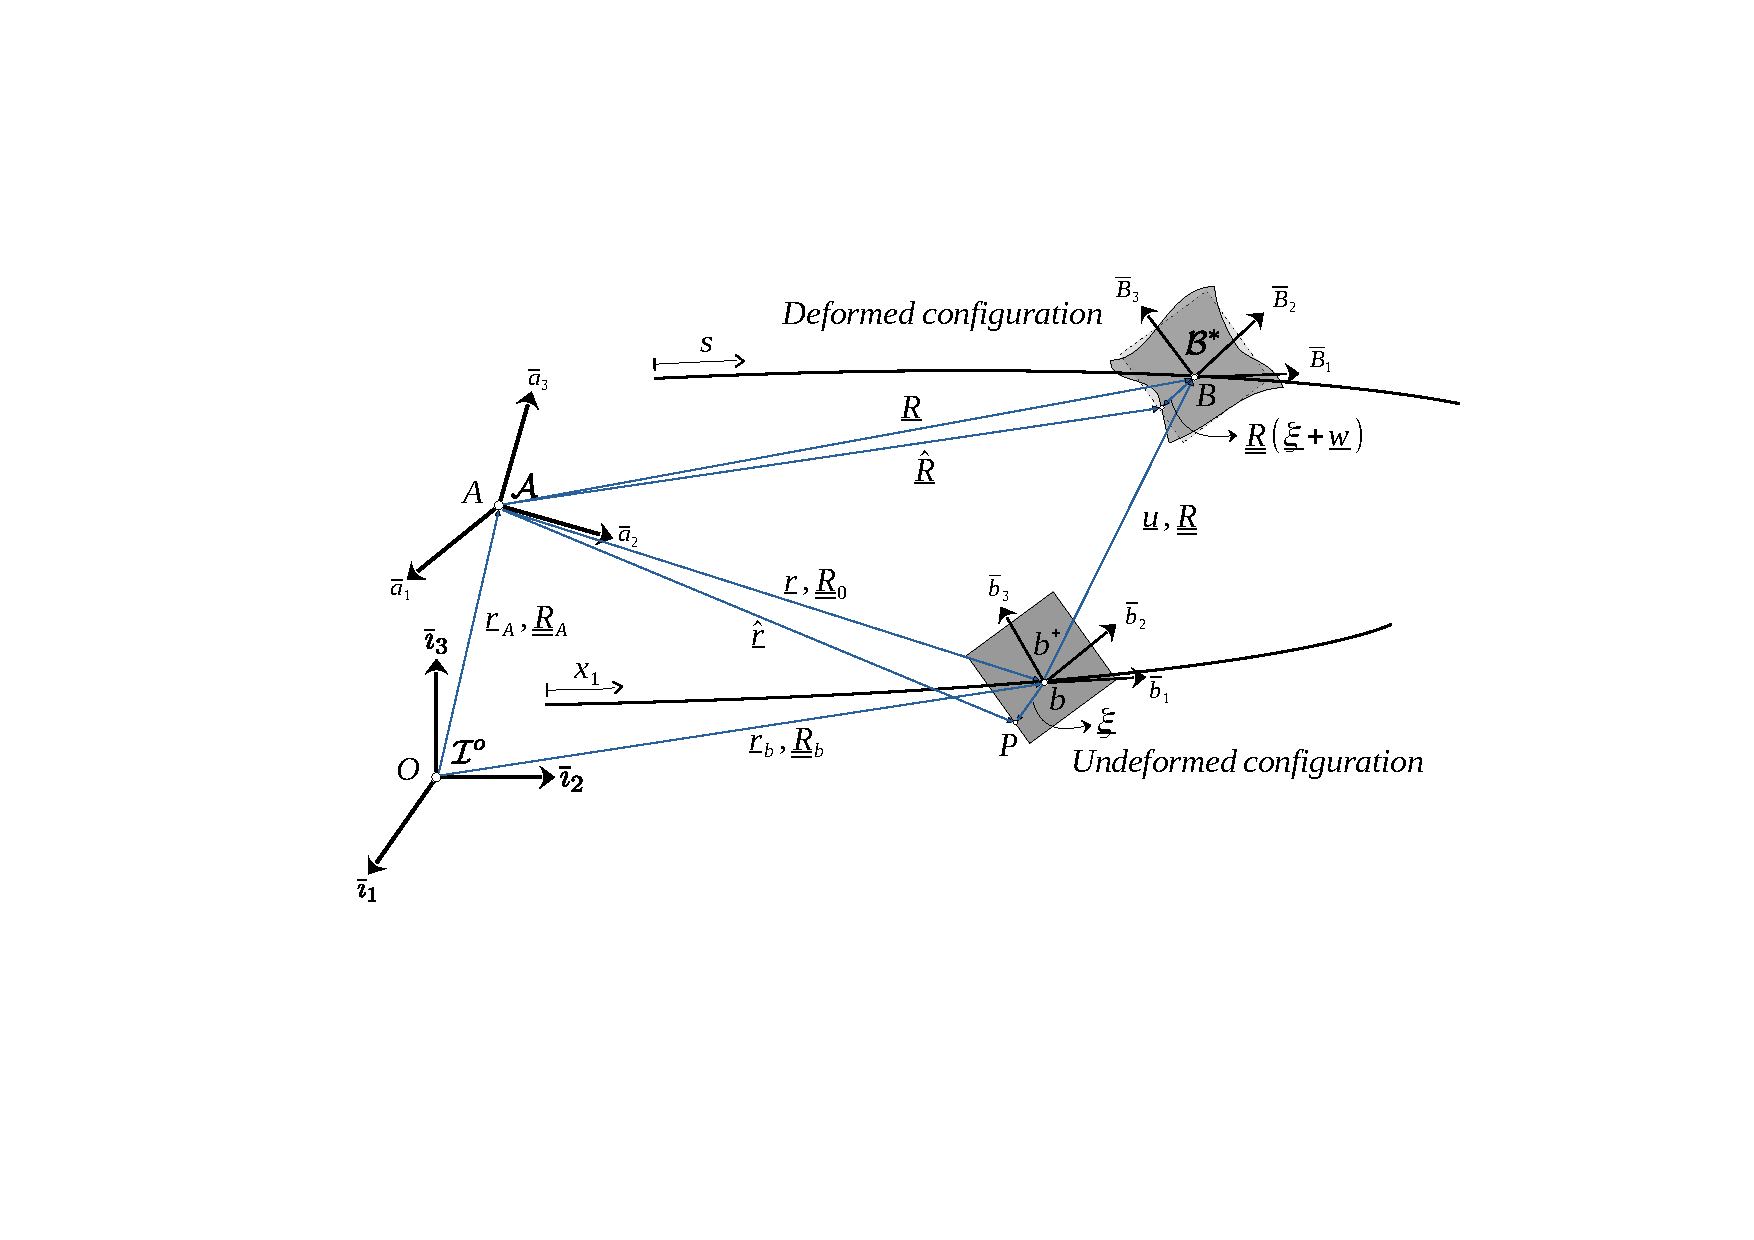
\includegraphics[width=0.95\linewidth,trim={6cm 5.7cm 5.5cm 4.5cm}, clip]{figures/kinematics.pdf}
        \label{fig_beam_kin}
	\end{center}
    \legend{Source: the author.}
\end{figure}

In the undeformed configuration, the beam is idealized as an initially twisted and curved reference line with a defined cross-section at each point, shown as a gray rectangle in the figure. The curvilinear coordinate $\xo$ defines an intrinsic parametrization of the reference line, i.e., denotes the arc-length along it. In this undeformed configuration, an orthonormal basis $\bp(\xo,t) = [\uvec{b}_1(\xo,t),\uvec{b}_2(\xo,t),\uvec{b}_3(\xo,t)]$, called the \textit{undeformed beam basis}, is defined at each point $b$ along the reference line. Tensor components resolved in basis $\bp$ are denoted with a superscript $(\cdot{})^{+}$. Each basis $\bp(\xo,t)$ is fixed with respect to basis $\A$, that is, it does not change over time for an observer at frame $\mathcal{F^A}$, but may do for an observer at frame $\mathcal{F^I}^{\circ}$. Vector $\uvec{b}_1$ is defined to be the unit tangent vector to the reference line, whereas unit vectors $\uvec{b}_2$ and $\uvec{b}_3$ span the plane of the cross-section. The position vector of a point $b$ along the reference line, with respect to point $A$, is denoted $\r$, and the components of the rotation tensor that brings basis $\A$ to basis $\bp(\xo,t)$, resolved in basis $\A$, are denoted $\Rz(\xo,t)$. Also, the position vector of a material point $P$ on a particular cross-section relative to the point $b$, where that cross-section is intersected by the reference line, is denoted by vector $\vect{\xi}(x_1,x_2,x_3,t) = x_2 \uvec{b}_2 + x_3 \uvec{b}_3$, in which $x_2$ and $x_3$ represent the material coordinates along vectors $\uvec{b}_2$ and $\uvec{b}_3$, respectively. Notice that $\r$, $\uvec{b}_1$, $\uvec{b}_2$, $\uvec{b}_3$, and $\vect{\xi}$ are all vector components \textit{resolved in basis} $\A$. Therefore, the position vector of point $P$ with respect to point $A$ is
\begin{equation}
    \hat{\r}(\xo,x_2,x_3,t) = \r(\xo,t) + \vect{\xi}(x_1,x_2,x_3,t) \ \ .
    \label{eq:r_hat}
\end{equation}

Upon deformation, each point $b$ of the beam's undeformed reference line moves to a point $B$, whose loci define a new reference line in the deformed configuration. The curvilinear coordinate $s(\xo,t)$ represents arc-length along this deformed reference line. At each point $B$ is defined an orthonormal basis $\B*(\xo,t) = [\uvec{B}_1(\xo,t),\uvec{B}_2(\xo,t),\uvec{B}_3(\xo,t)]$, called the \textit{deformed beam basis}, and tensor components resolved in that basis are denoted with a superscript $(\cdot{})^{*}$. The total deformation of the beam can be decomposed into \textbf{(i)} a rigid-body translation of the reference line, \textbf{(ii)} a rigid-body rotation of the cross-section, and \textbf{(iii)} warping displacements including in- and out-of-plane deformations of the cross-section, whose components resolved in basis $\A$ are given as $\vect{w}(\xo,x_2,x_3,t) = w_1(\xo,x_2,x_3,t) \uvec{b}_1 + w_2(\xo,x_2,x_3,t) \uvec{b}_2 + w_3(\xo,x_2,x_3,t) \uvec{b}_3$. To be uniquely defined, the warping displacement field must be orthogonal to the rigid-body motion, so that $\uvec{B}_1$ is orthogonal to the average plane of the deformed cross-section (shown in a dotted outline, light gray rectangle in Figure \ref{fig_beam_kin}), and $\uvec{B}_2$ and $\uvec{B}_3$ span that plane \cite{bauchau2011flexible}. Basis $\B*(\xo,t)$ is thus defined and it can be noticed that $\uvec{B}_1$ is not, in general, tangent to the deformed beam's reference line. The rigid-body translation of a point $b$ to a point $B$ is given by vector $\vect{u}(\xo,t)$, and the components of the rotation tensor that brings basis $\bp$ to basis $\B*$, are denoted $\R(\xo,t)$, both resolved in basis $\A$, so that tensor $\R$ is associated with the rigid-body rotation of the cross-section. The position vector of point $B$ with respect to point $A$ thus is $\vect{R} = \r + \vect{u}$, and the position vector of point $P$ with respect to point $A$ in the deformed configuration, $\hat{\vect{R}}(\xo,x_2,x_3,t)$, defines the \textit{displacement field} as
\begin{align}
    \hat{\vect{R}} 
    &= \vect{R} + \R(\vect{\xi} + \vect{w})
    \nonumber
    \\
    &= \r + \vect{u} + w_1 \uvec{B}_1 + (w_2 + x_2) \uvec{B}_2 + (w_3 + x_3) \uvec{B}_3 \ \ ,
    \label{eq:R_hat}
\end{align}
where was used the fact that the \textit{transformation rule for change of basis operations} on first-order tensors \cite{bauchau2011flexible} yields
\begin{equation}
    \uvec{B}_i = \R \uvec{b}_i, \; (i = 1,2,3) \ \ .
    \label{eq:B_i}
\end{equation}

The warping displacements, being the only unknowns dependent on $x_2$ and $x_3$ in \cref{eq:R_hat}, can be eliminated through the process of dimensional reduction, and later found from the two-dimensional cross-sectional analysis. That, however, is out of the scope of our intentions. 

\subsection{Velocity field}

Now that the displacement field is defined, it is possible to find the velocity field by straightforward time differentiation. For that matter, the influence of warping on the inertial velocity of a point can be neglected, since asymptotic methods show that it is small, i.e., of the order of the strain compared to the order of the cross-section dimension \cite{hodges2006nonlinear}. It is important to note that the concept of  ``inertial velocity'' means ``the velocity with respect to an inertial frame'', in this case, $\mathcal{F^I}^{\circ}$, and it is a vector that may be resolved in any basis. Referring back to \cref{fig_beam_kin}, the components of the displacement field with suppressed warping displacements, resolved in the inertial basis $\Io$, are
\begin{align}
    \hat{\vect{R}}^{\circ}_0 
    &= \hat{\vect{R}}^{\circ} - \vect{w}^{\circ} \nonumber 
    \\
    &= \rbo + \uo + x_2\uvec{B}_2^\circ + x_3\uvec{B}_3^\circ \nonumber 
    \\
    &= \rbo + \Rbp\uplus + \lp\Rbo\Rp\rp\xis 
    \label{eq:R_hat_0_partial} 
    \\
    &= \rbo + \Rbp\uplus + \lp\Ro\Rbo\rp\xis \ \ ,
    \label{eq:R_hat_0}    
\end{align}
where $\rbo$ are the components of the position vector of a point $b$ with respect to point $O$, resolved in basis $\Io$, $\Rbo$ are the components of the rotation tensor that brings basis $\Io$ to basis $\bp$, resolved in basis $\Io$, and $\xis = \{0, x_2, x_3\}^\T$ are the components of the position of point $P$ embedded in the cross-section, resolved in basis $\mathcal{B}^{*}$. Notice that, using the transformation rule for second-order tensors \cite{bauchau2011flexible},
\begin{align}
    \Rbp = \RboT\Rbo\Rbo = \Rbo \ \ ,
    \label{eq:Rbp}    
\end{align}
that is, the components of a rotation tensor resolved in the two bases it relates, are identical. Furthermore, in \cref{eq:R_hat_0_partial}, every tensor has been resolved in the basis in which it is ``most naturally'' described, whereas in \cref{eq:R_hat_0}, the orthogonality property of the rotation tensor and the transformation rule were used to write 
\begin{align}
    \Rbo\Rp = \Rbo\lp\RboT\Ro\Rbo\rp = \Ro\Rbo \ \ ,
\label{eq:RboRp}    
\end{align}
which shows that the order in which the rotation tensors appear in a \textit{composition of rotations} depends on the basis in which they are resolved \cite{bauchau2011flexible}.

Taking a time derivative of \cref{eq:R_hat_0} yields the components of the inertial velocity of an arbitrary point $P$, i.e., the \textit{velocity field}, resolved in basis $\Io$, as
\begin{align}
    \vPo &= \dot{\hat{\vect{R}}}^{\circ}_0 \nonumber 
    \\
    &= \rbodot + \lp\Rbp\uplus\rp\dotout + \lp\Ro\Rbo\rp\dotout \xis \nonumber 
    \\
    &= \rbodot + \Rbpdot\uplus + \Rbp\updot + \lp\Ro\Rbo\rp\dotout \lp\Ro\Rbo\rp^\T \lp\Ro\Rbo\rp \xis \nonumber 
    \\
    &= \rbodot + \Rbpdot\RbpT\Rbp\uplus + \Rbp\updot + \Omtilo \lp\Ro\Rbo\rp \xis \nonumber
    \\
    &= \vbo + \omtilo\uo + \Rbp\updot + \Omtilo\xio \ \ ,
    \label{eq:v_P_o}    
\end{align}
in which $\vbo =  \rbodot$ is the inertial velocity vector of basis $\bp$, whereas the inertial angular velocity vector of the $\bp$ basis, $\omo$, and the inertial angular velocity of the $\mathcal{B}^{*}$ basis, $\Omo$, are defined as
\begin{align}
    \omo &\coloneqq \axial\lp\Rbodot\RboT\rp =
    \axial\lp\Rbpdot\RbpT\rp \ \ ,
    \label{eq:omega_def}
    \\
    \Omo &\coloneqq \axial\lb\lp\Ro\Rbo\rp\dotout \lp\Ro\Rbo\rp^\T\rb =
    \axial\lb\lp\Rbp\Rp\rp\dotout \lp\Rbp\Rp\rp^\T\rb \ \ ,
    \label{eq:Omega_def}    
\end{align}
in which the notations $\dot{(\cdot)}$ and $(\cdot)\dotout$ both denote a derivative with respect to time. Moreover, from the discussion in Section \ref{sec:notation}, it is clear that Eqs.~\eqref{eq:omega_def} and \eqref{eq:Omega_def} are equivalent to
\begin{align}
    \omtilo &\coloneqq \Rbodot\RboT =
    \Rbpdot\RbpT \ \ ,
    \label{eq:omegatil_def}
    \\
    \Omtilo &\coloneqq \lp\Ro\Rbo\rp\dotout \lp\Ro\Rbo\rp^\T =
    \lp\Rbp\Rp\rp\dotout \lp\Rbp\Rp\rp^\T \ \ .
    \label{eq:Omegatil_def}    
\end{align}

Vectors $\vbo$ and $\omo$ in \cref{eq:v_P_o} therefore define the motion of basis $\bp$ with respect to basis $\Io$, but they must eventually be expressed in terms of the inertial velocity and inertial angular velocity vectors of basis $\A$, denoted $\vAo$ and $\omAo$, respectively, which are assumed to be known from the onset of the analysis. To that end, an important fact to realize is that because the angular velocity is a \textit{free vector} \cite{bauchau2011flexible}, the components of $\om$ represent not only the inertial angular velocity vector of basis $\bp$, but also that of basis $\A$, since the former basis is fixed concerning the latter. To see that, first notice that $\Rbo$ is obtained from a composition of rotations as 
\begin{equation}
    \Rbo = \Rzo\RAo = \RA\Rz \rightarrow \RboT = \RzT\RAT \ \ ,
    \label{eq:RboT}
\end{equation}
which implies
\begin{align}
    \Rbodot = \lp\RA\Rz\rp\dotout = \RAdot\Rz + \RA\cancelto{\zthree}{\Rzdot} = \RAdot\Rz \ \ ,
    \label{eq:Rbodot}
\end{align}
where the fact that $\Rzdot = \zthree$ was used, since basis $\bp$ is fixed with respect to basis $\A$. Now, using \cref{eq:RboT,eq:Rbodot} to perform a change of basis operation on \cref{eq:omegatil_def} yields
\begin{align}
    \omtil = \RAT\omtilo\RA = \RAT\Rbodot\RboT\RA =
    \RAT\lp\RAdot\Rz\rp\lp\RzT\RAT\rp\RA = \RAT\RAdot \eqdef \omAtil \ \ ,
    \label{eq:omtilo_omtilA}
\end{align}
thus completing the argument. 

In contrast, the components of $\vbo$ have to be obtained from a relative velocity analysis, since it is a \textit{bound vector} \cite{bauchau2011flexible}. Accordingly, consider that $\rbo$ may be written as
\begin{align}
    \rbo = \rAo + \ro \ \ .
    \label{eq:rbo}
\end{align}

Taking a time derivative of this expression leads to
\begin{align}
    \rbodot = \vbo &= \rAdoto + \rdoto
    \nonumber 
    \\
    &= \vAo + \lp\RA\r\rp\dotout
    \nonumber
    \\
    &= \vAo + \RAdot\r + \RA\cancelto{\zv}{\rdot}
    \nonumber
    \\
    &= \vAo + \RAdot\RAT\ro
    \nonumber
    \\
    &= \vAo + \omAtilo\ro \ \ ,
    \label{eq:vbo}
\end{align}
in which $\rAdoto = \vAo$, $\omAtilo \coloneqq \RAdot\RAT$, and the fact that $\rdot = \vect{0}$ was used, because basis $\bp$ is fixed with respect to basis $\A$. Using \cref{eq:vbo}, the components of the inertial velocity of basis $\bp$, resolved in basis $\A$, can be written in terms of known quantities only as
\begin{align}
    \vb &= \RAT\vbo
    \nonumber 
    \\
    &= \RAT \lp\vAo + \omAtilo\ro\rp
    \nonumber 
    \\
    &= \RAT\vAo + \RAT\omAtilo\RA\r
    \nonumber 
    \\
    &= \RAT\lp\vAo + \omAtilo\RA\r\rp \ \ .
    \label{eq:vb}
\end{align}

Going back to the velocity field expression, it is illustrative to notice that the first three terms on the right-hand side of \cref{eq:v_P_o} denote the inertial velocity vector of basis $\mathcal{B}^{*}$, resolved in basis $\Io$, that is,
\begin{align}
    \Vo &= \vbo + \omtilo\uo + \Rbp\updot \ \ ,
    \label{eq:V_o}
\end{align}
where the terms $\vbo$ and $\omtilo\uo$ account for the velocity components due to the translation and rotation, respectively, of basis $\bp$ with respect to basis $\Io$, and $\Rbp\updot$ represents the velocity of basis $\mathcal{B}^{*}$ with respect to basis $\bp$. The components of $\V$ are most naturally expressed in the deformed beam basis, which can thus be written in terms of tensor components resolved in the undeformed beam basis as
\begin{align}
    \Vs &= \lp\Rbp\Rp\rp^\T \Vo
    \label{eq:V_star_initial} 
    \\
    &= \lp\RpT\RbpT\rp \lp\vbo + \omtilo\uo + \Rbp\updot\rp \nonumber 
    \\
    &= \lp\RpT\RbpT\rp\Rbp \lp\vbplus + \omtilp\uplus + \updot\rp \nonumber 
    \\
    &= \RpT \lp\vbplus + \omtilp\uplus + \updot\rp \ \ .
    \label{eq:V_star}
\end{align}

Similarly, that can also be done for the vector product operator of the angular velocity vector of basis $\B*$, using \cref{eq:Omegatil_def} to find
\begin{align}
    \Omtils &= \lp\Rbp\Rp\rp^\T\Omtilo\lp\Rbp\Rp\rp \label{eq:Omegatil_initial} 
    \\
    &= \lp\Rbp\Rp\rp^\T\lp\Rbp\Rp\rp\dotout \lp\Rbp\Rp\rp^\T\lp\Rbp\Rp\rp \nonumber 
    \\
    &= \RpT\RbpT\lp\Rbpdot\Rp + \Rbp\Rpdot\rp \nonumber 
    \\
    &= \RpT\lp\RbpT\Rbpdot\rp\Rp + \RpT\Rpdot \nonumber 
    \\
    &= \RpT\omtilp\Rp + \RpT\Rpdot \label{eq:Omegatil_star_partial} 
    \\
    &= -\lp\RpT\Rpdot\rp^\T + \RpT\omtilp\Rp \nonumber 
    \\
    &= -\RpTdot\Rp + \RpT\omtilp\Rp \ \ .
    \label{eq:Omegatil_star}
\end{align}
where the property that $\til{a}^\T = -\til{a}$, for any $\til{a}$, was used to write $\RpT\Rpdot = -\lp\RpT\Rpdot\rp^\T$, and the fact that $\omtilp = \RbpT\Rbpdot$, as can be seen by performing a change of basis operation on \cref{eq:omegatil_def}. Equations ~\eqref{eq:V_star} and \eqref{eq:Omegatil_star} express the so-called \textit{generalized velocity-displacement relationships}. 

To deal with rotation, it will later be necessary to express the angular velocity vector, $\Oms$, in terms of the time derivative of a chosen set of rotation parameters. From  \cref{eq:Omegatil_star_partial}, it can be concluded that
\begin{align}
    \Oms &= \axial\lp\RpT\Rpdot\rp + \RpT\omp \nonumber 
    \\
    &= \HpT\ppdot + \RpT\omp 
    \label{eq:Omega_star_rotparp} 
    \\
    &= \lp\RzT\HT\Rz\rp \lp\RzT\pdot\rp + \lp\RzT\RT\Rz\rp \lp\RzT\om\rp \nonumber \\
    &= \RzT\lp\HT\pdot+\RT\om\rp \ \ ,
    \label{eq:Omega_star_rotpar}
\end{align}
where $\H$ is the so-called \textit{tangent operator tensor}, and $\p$ is the \textit{rotation parameters vector} \cite{bauchau2011flexible} associated with the rotation tensor $\R$. The tangent operator has the function of transforming between the time derivatives of rotation parameters and angular velocities, and analogously, between the spatial derivatives of rotation parameters and curvatures, see \cref{sec:strain}. It is important to recognize that $\p$, being a \textit{vectorial parametrization of rotation}, follows the tensor transformation rule, and thus,
\begin{align}
    \p &= \Rz\pplus \ \ .
    \label{eq:rotpar}
\end{align}

Finally, a compact expression can be written for the components of the inertial velocity field resolved in basis $\B*$, by applying the transformation rule to $\vP$ and using \cref{eq:V_o,eq:V_star_initial,eq:Omegatil_initial} to find
\begin{align}
    \vPs &= \lp\Rbp\Rp\rp^\T \vPo \nonumber 
    \\
    &= \lp\Rbp\Rp\rp^\T \lp \Vo + \Omtilo\xio \rp \nonumber 
    \\
    &= \Vs + \lp\Rbp\Rp\rp^\T\Omtilo\lp\Rbp\Rp\rp\lp\Rbp\Rp\rp^\T\xis \nonumber 
    \\
    &= \Vs + \Omtils\xis \ \ ,
    \label{eq:v_P_star}
\end{align}
where it is noted that $\Vs$ and $\Oms$ are rightfully called the \textit{sectional velocity}, and \textit{sectional angular velocity} vectors, respectively, of the deformed beam, and $\xis$ is the \textit{sectional position} of an arbitrary point $P$ of the beam.


% Section: Strain measures
\section{Strain measures}
\label{sec:strain}

The purpose of the present section is to define the one-dimensional \textit{generalized strain measures} through \textit{generalized strain-displacement relations}, in order to later formulate the strain energy of the beam due to deformation. \citeonline{hodges2006nonlinear} expresses the components of the so-called \textit{force-strains} vector, $\gam$, and \textit{moment-strains} vector, $\kap$, resolved in basis $\A$, as
\begin{align}
    \gam 
    &= \RT\lp\r+\u\rp^\prime-\r^\prime \ \ ,
    \label{eq:gamma_def}
    \\
    \kap &= \RT\K - \k \ \ ,
    \label{eq:kappa_def}
\end{align}
where notation $(\cdot{})^{\prime}$ denotes differentiation with respect to $\xo$, and the \textit{curvature vectors} of the undeformed and deformed beam's reference lines are respectively defined as 
\begin{align}
    \k &\coloneqq \axial\lp\Rz^{\prime}\RzT\rp \ \ ,
    \label{eq:k_def}
    \\
    \K &\coloneqq \axial\lb\lp\R\;\Rz\rp^{\prime} \lp\R\;\Rz\rp^\T\rb =
    \axial\lb\lp\Rz\Rp\rp^{\prime} \lp\Rz\Rp\rp^\T\rb \ \ .
    \label{eq:K_def}    
\end{align}

The strain vectors are measures of deformation: \cref{eq:gamma_def} expresses that the force-strains vector is the difference between the unit tangent vector of the deformed beam's reference line, $\lp\r+\u\rp^\prime$, pulled back to the undeformed beam basis by pre-multiplication by $\RT$ (this is the definition of the ``pull back'' operation), and the unit tangent vector of the undeformed beam's reference line, $\rprime = \uvec{b}_1$, since $\uvec{b}_1$ was defined to be so. Also, \cref{eq:kappa_def} put into words means that the moment-strains vector is the difference between the curvature of the deformed beam's reference line, $\K$, pulled back to the undeformed beam basis, and the curvature of the undeformed beam's reference line, $\k$.

\subsection{Force-strains}

The force-strains are so called because their components resolved in the undeformed beam basis, $\bp$, are \textit{energetically-conjugate} to the components of the sectional force resultants (which will be defined in \cref{sec:ede}) resolved in the deformed beam basis, $\B*$, i.e., their scalar product yields the strain energy stored in the beam per unit length. Therefore, the strain vectors must be expressed in basis $\bp$. To do that, more convenient relations for $\rprime$ and $\lp\r+\u\rp^\prime$ must be found to rewrite the force-strains. Consider the transformation rule for first-order tensors applied to $\r$, which yields $\r = \Rz\rplus$. Therefore,
\begin{align}
    \RzT\rprime &= \RzT\lp\Rz\rplus\rp^\prime \nonumber 
    \\
    &= \RzT\Rzp\rplus+\RzT\Rz\rpprime  \nonumber 
    \\
    &= \rpprime + \RzT\lp\Rzp\RzT\rp\Rz\rplus \nonumber
    \\
    &= \rpprime + \ktilp\rplus \ \ ,
    \label{eq:Rztrprime}
\end{align}
where the transformation rule for second-order tensors was used to write 
\begin{align}
    \ktilp = \RzT\ktil\Rz = \RzT\lp\Rzp\RzT\rp\Rz = \RzT\Rzp \ \ .
    \label{eq:ktilp}
\end{align}

An important simplification arises from the fact that $\uvec{b}_1$ is tangent to the undeformed beam's reference line, i.e., $\rprime = \uvec{b}_1$, because it implies that 
\begin{align}
    \RzT\rprime &= \RzT\uvec{b}_1 \nonumber 
    \\ 
    &= \uvec{b}^{+}_1 \nonumber 
    \\
    &= \{1, 0, 0\}^\T \nonumber 
    \\
    &= \aone \ \ ,
    \label{eq:Rztrprime_simple}
\end{align}
which is vector $\uvec{b}_1$ as seen by an observer at the origin of basis $\bp$, or vector $\aone$ as seen by an observer at the origin of $\A$, and so on. Using this finding, it is straightforward to show, in analogy to \cref{eq:Rztrprime}, that
\begin{align}
    \RzT\lp\r+\u\rp^\prime &= \lp\rpprime+\upprime\rp + \ktilp\lp\rplus+\uplus\rp \nonumber 
    \\
    &= \aone + \upprime + \ktilp\uplus \ \ ,
    \label{eq:Rztruprime}
\end{align}

Now, with the help of Eqs.~\eqref{eq:gamma_def}, \eqref{eq:Rztrprime_simple} and \eqref{eq:Rztruprime}, the strain-displacement relations for the force-strains may be written as
\begin{align}
    \gamp 
    &= \RzT\gam \nonumber 
    \\
    &= \RzT\RT \lp\r+\u\rp^\prime-\RzT\r^\prime \nonumber 
    \\
    &= \RzT\RT \lp\Rz\aone+\uprime\rp-\aone 
    \label{eq:gamp_A} 
    \\
    &= \RzT\RT\Rz\RzT\lp\rprime+\uprime\rp-\aone \nonumber 
    \\
    &= \RpT\lp\uvec{b}^{+}_1 + \upprime + \ktilp\uplus\rp - \uvec{b}^{+}_1 \ \ ,
    \label{eq:gamp_b}
\end{align}
where it can be noticed that in \cref{eq:gamp_A} the variables in the right-hand side have been expressed in terms of tensor components resolved only in basis $\A$, whereas in \cref{eq:gamp_b}, they are resolved only in basis $\bp$. Notice that because \cref{eq:gamma_def} assumes small strains, $\gamp = \{\gamma_{11},2\gamma_{12},2\gamma_{13}\}^\T$ where $\gamma_{11}$, $2\gamma_{12}$ and $2\gamma_{13}$ represent the \textit{engineering strains}, i.e., the \textit{axial extension strain} along $\uvec{b}_1$, and \textit{shear strains} of the reference line in the directions of $\uvec{b}_2$ and $\uvec{b}_3$, respectively.

\subsection{Moment-strains}

Analogously to the force-strains, the components of the moment-strains resolved in basis $\bp$ are energetically-conjugate to the components of the sectional moment resultants resolved in basis $\B*$.
The strain-displacement, or rather, strain-rotation relationship for the moment-strains may be resolved in basis $\bp$, starting from \cref{eq:kappa_def} to write
\begin{align}
    \kapp 
    &= \RzT\kap \nonumber 
    \\
    &= \RzT\RT\K-\RzT\k \nonumber 
    \\
    &= \lp\R\;\Rz\rp^\T\K - \RzT\k \nonumber 
    \\
    &= \Ks - \kp \ \ ,
    \label{eq:kappa_plus}
\end{align}
where $\kp = \{k_1,k_2,k_3\}^\T$, in which the measure numbers $k_1$, $k_2$ and $k_3$ represent the curvatures (per unit length) in the directions of $\uvec{b}_1$, $\uvec{b}_2$, and $\uvec{b}_3$, respectively, of the undeformed beam's reference line. Similarly, $\Ks = \{K_1,K_2,K_3\}^\T$, in which $K_1$, $K_2$ and $K_3$ represent these corresponding quantities for the deformed beam's reference line, when its axial stretching is excluded, in the directions of $\uvec{B}_1$, $\uvec{B}_2$, and $\uvec{B}_3$, respectively. Thus, the measure number $\kappa_1 = K_1-k_1$ is the \textit{elastic twist curvature}, and $\kappa_2 = K_2-k_2$ and $\kappa_3 = K_3-k_3$ are \textit{elastic bending curvatures} along $\uvec{b}_2$ and $\uvec{b}_3$, such that $\kapp = \{\kappa_1,\kappa_2,\kappa_3\}^\T$. 

A useful expression for the vector product operator of $\Ks$ in terms of tensor components resolved in basis $\bp$ can be found using Eqs.~\eqref{eq:K_def} and \eqref{eq:ktilp},
\begin{align}
    \Ktils 
    &= \lp\Rz\Rp\rp^\T\Ktil\lp\Rz\Rp\rp \nonumber 
    \\
    &= \lp\Rz\Rp\rp^\T\lp\Rz\Rp\rp^{\prime} \lp\Rz\Rp\rp^\T\lp\Rz\Rp\rp \nonumber
    \\
    &= \lp\RpT\RzT\rp \lp\Rzp\Rp+\Rz\Rpprime\rp \nonumber 
    \\
    &= \RpT\lp\RzT\Rzp\rp\Rp + \RpT\Rpprime \nonumber 
    \\
    &= \RpT\ktilp\Rp + \RpT\Rpprime \label{eq:Ktils1} 
    \\
    &= -\lp\RpT\Rpprime\rp^\T + \RpT\ktilp\Rp \nonumber 
    \\
    &= -\RpprimeT\Rp + \RpT\ktilp\Rp \ \ ,
    \label{eq:Ktils}
\end{align}
where the similarity with \cref{eq:Omegatil_star} for the sectional angular velocity becomes clear. Just like in the case of the angular velocities, it later becomes imperative to introduce rotation parameters to express the curvature quantities. It follows directly from \cref{eq:Ktils1} that
\begin{align}
    \Ks 
    &= \axial\lp\RpT\Rpprime\rp + \RpT\kp \nonumber 
    \\
    &= \HpT\ppprime + \RpT\kp \ \ ,
    \label{eq:Ks_rotpar}
\end{align}
which implies that \cref{eq:kappa_plus} can be recast as
\begin{align}
    \kapp &= \HpT\ppprime + \RpT\kp - \kp \ \ ,
    \label{eq:kappa_plus2}
\end{align}
where $\kapp$ has been written in terms of tensor components resolved in basis $\bp$. To write the simplest form of $\kapp$ in terms of tensor components resolved in basis $\A$, it is more convenient to first find such an expression for its vector product operator. Starting from \cref{eq:kappa_plus}, and using Eqs.~\eqref{eq:K_def} and \eqref{eq:ktilp}, 
\begin{align}
    \kapptil
    &= \Ktils - \ktilp \nonumber
    \\
    &= \lp\R\;\Rz\rp^\T\lb\lp\R\;\Rz\rp^\prime\lp\R\;\Rz\rp^\T\rb\lp\R\;\Rz\rp - \RzT\lp\Rzp\RzT\rp\Rz \nonumber 
    \\
    &= \lp\R\;\Rz\rp^\T\lp\R\;\Rz\rp^\prime - \RzT\Rzp \nonumber 
    \\
    &= \RzT\RT\lp\R\;\Rzp+\Rprime\Rz\rp - \RzT\Rzp \nonumber 
    \\
    &= \RzT\Rzp + \RzT\RT\Rprime\Rz - \RzT\Rzp \nonumber 
    \\
    &= \RzT\RT\Rprime\Rz \ \ ,
    \label{eq:kappatil_plus}
\end{align}
which implies that
\begin{align}
    \kapp
    &= \RzT \cdot \axial\lp\RT\Rprime\rp \nonumber 
    \\
    &= \RzT\HT\pprime \ \ .
    \label{eq:kappa_plus_A}
\end{align}

It must pointed out that for these six strain measures considered, three force-strains and three moment-strains, the current developments yield a so-called \textit{Timoshenko theory} of beams, which is valid specifically for what \citeonline{hodges2006nonlinear} calls ``class $\mathcal{R}$'' beams (beams of solid, or thin-walled, closed cross-sections) and ``class $\mathcal{S}$'' beams (beams of strip-like cross-sections). The treatment of ``class $\mathcal{T}$'' beams (thin-walled beams of open cross-section, e.g., ``I'' ``T'' or ``C'' cross-sections) involves the consideration of an additional strain measure, accounting for the out-of-plane warping of the cross-section caused by torsion, yielding a so-called \textit{Vlasov theory}. The present formulation also does not account for the \textit{trapeze effect} \cite{hodges2006nonlinear}, which demands the establishment of third-order terms of the generalized strains in the expression for the strain energy, and can be particularly important for classes $\mathcal{S}$ and $\mathcal{T}$ beams under axial loads. Incorporation of such Vlasov and trapeze effects will be the object of future work, since the structures of HALE aircraft are typically beams of classes $\mathcal{R}$ or $\mathcal{S}$ under low axial loads.


\section{Equations of dynamic equilibrium}
\label{sec:ede}

With the kinematical and generalized strain-displacement relationships from \cref{sec:kin,sec:strain} at hand, it is now possible to develop the equations of dynamic equilibrium. These are derived from Hamilton's principle, which can be stated as
\begin{equation}
    \intt\intl \left\{\delta\lp\mathcal{K}-\mathcal{U}\rp+\overline{\delta \mathcal{W}}_{\textnormal{ext}}\right\} \d \xo\;\d t = \overline{\delta\A} \ \ ,
    \label{eq:hamilton}
\end{equation}
where $t_1$ and $t_2$ represent initial and final instances of a time interval, $l$ is the length of the beam, $\delta$ is the \textit{variational operator} (when no superscript is used, the variation is taken in basis $\A$), $\mathcal{K}$ and $\mathcal{U}$ are the \textit{kinetic energy} and \textit{strain energy} of the beam per unit length, respectively, $\overline{\delta \mathcal{W}}_{\textnormal{ext}}$ is the \textit{virtual work} of applied loads per unit length of the beam, and $\overline{\delta\A}$ is the \textit{virtual action} applied at the ends of the beam, at the initial and final times. The notation $\overline{(\cdot)}$, with the bar extending over the variational operator in $\overline{\delta \mathcal{W}}_{\textnormal{ext}}$ and $\overline{\delta\A}$, is used to denote the fact that these terms do not necessarily represent variations of a functional, since the applied loads may not be integrable (non-conservative loads in general, e.g., follower loads, friction forces, etc.). The task now resumes to that of finding the variations in \cref{eq:hamilton}.

\subsection{Strain energy}

The form of the strain energy per unit length is assumed to be known as a function of the generalized strain measures, that is, $\mathcal{U} = \mathcal{U}\lp\gamp,\kapp\rp$. Therefore, its variation can be written as
\begin{align}
    \delta\mathcal{U} &= \delta\gampT\lp\del{\mathcal{U}}{\gamp}\rp^\T + \delta\kappT\lp\del{\mathcal{U}}{\kapp}\rp^\T \nonumber 
    \\
    &= \delta\gampT\Fs + \delta\kappT\Ms \ \ ,
    \label{eq:delU}
\end{align}
where the components of the \textit{sectional force resultants} and of the \textit{sectional moment resultants} vectors, resolved in the $\B*$ basis, are respectively defined as
\begin{align}
    \Fs &\coloneqq \lp\del{\mathcal{U}}{\gamp}\rp^\T \ \ , \label{eq:force_res} 
    \\
    \Ms & \coloneqq \lp\del{\mathcal{U}}{\kapp}\rp^\T \ \ ,
    \label{eq:mom_res}
\end{align}
where it is noted that the transpose operators stem from the fact that the derivative of a scalar with respect to a vector is represented by a row matrix in vector calculus. In \cref{eq:force_res}, $\Fs = \{F_1,F_2,F_3\}^\T$, in which the measure number $F_1$ represents the axial force along $\uvec{B}_1$, whereas $F_2$ and $F_3$ are the shear forces along $\uvec{B}_2$ and $\uvec{B}_3$, respectively. Similarly, in \cref{eq:mom_res}, $\Ms = \{M_1,M_2,M_3\}^\T$, in which $M_1$ represents the twisting moment acting in the direction of $\uvec{B}_1$, whereas $M_2$ and $M_3$ are bending moments along $\uvec{B}_2$ and $\uvec{B}_3$, respectively. 

The generalized sectional force resultants are related to the generalized strains through the so-called \textit{generalized force-strain}, or \textit{geometry-material constitutive relations}, which may be written as
\begin{align}
    \begin{Bmatrix}
    \gamp \\ \kapp
    \end{Bmatrix}
	= \Compliance
	\begin{Bmatrix}
    \Fs \\ \Ms
    \end{Bmatrix}
    \rightarrow
    \begin{Bmatrix}
    \Fs \\ \Ms
    \end{Bmatrix}
	= \Stiff
	\begin{Bmatrix}
    \gamp \\ \kapp
    \end{Bmatrix} \ \ ,
    \label{eq:constitutive}
\end{align}
in which the $6 \times 6$ matrix $\Compliance$ is the beam's \textit{sectional compliance matrix}, and  $\Stiff = \mathcal{\tens{C}}^{*^{-1}}$ is the  \textit{sectional stiffness matrix}, whose terms depend on the cross-section's \textit{geometric properties}, such as area and area's second moments of inertia, and \textit{material's elastic properties}, such as Young's and shear moduli. The superscript $\lp\cdot\rp^*$ in these matrices, which are in fact representations of \textit{fourth-order tensors}, is used to denote the fact that they should be resolved in the deformed beam basis. Nonetheless, the assumption of small strains allows for the crucial simplification that the values known in the undeformed beam basis can actually be used. For isotropic beams of geometrically simple cross-sectional shapes, matrices $\Compliance$ and $\Stiff$ might be analytically computable, and may even be diagonal matrices. However, for beams of arbitrary cross-sectional shape and made of anisotropic materials, $\Compliance$ and $\Stiff$ may be fully populated, reflecting the coupling between all generalized strains and sectional forces, and might only be obtainable through a two-dimensional cross-sectional analysis, using programs such as \begin{small}VABS\end{small} \cite{hodges2006nonlinear} or GXBeam \cite{mcdonnell2022gxbeam}, the latter being an open source code.

\subsection{Kinetic energy}

The kinetic energy per unit length of the deformed beam may be written as
\begin{align}
    \mathcal{K} &= \frac{1}{2}\int_{S^*}\rho^*\vPsT\vPs\;\d S^* \ \ ,
    \label{eq:kinetic_energy}
\end{align}
where $\rho^*$ is the mass density (per unit volume) and $S^*$ is the cross-sectional area, both in the deformed configuration, and $\vPs = \Vs + \Omtils\xis$ are the components of the inertial, or absolute velocity of an arbitrary point $P$ in the beam, resolved in the deformed beam basis, as found in \cref{eq:v_P_star}. Notice that the small strains assumption leads to the important simplification that the values of $\rho^*$ and $S^*$ can assumed be to be equal to the known ones in the undeformed configuration, denoted $\rho$ and $S$, which are used henceforth. 

Substituting the above expressions into \cref{eq:kinetic_energy} yields
\begin{align}
    \mathcal{K} &= \frac{1}{2}\int_S \rho\lp\Vs + \Omtils\xis\rp^\T\lp\Vs + \Omtils\xis\rp \;\d S \nonumber 
    \\
    &= \frac{1}{2}\int_S \rho\lb \VsT\Vs + \VsT\Omtils\xis + \lp\Omtils\xis\rp^\T\Vs + \lp\Omtils\xis\rp^\T\lp\Omtils\xis\rp \rb\;\d S \nonumber 
    \\
    &= \frac{1}{2}\int_S \lb \rho\VsT\Vs + 2\rho\VsT\Omtils\xis + \rho \lp\xitilsT\Oms\rp^\T\lp\xitilsT\Oms\rp \rb\;\d S \nonumber 
    \\
    &= \frac{1}{2}\int_S \lb \rho\VsT\Vs + 2\rho\OmsT\VtilsT\xis +  \OmsT\rho\xitils\xitilsT\Oms \rb\;\d S \nonumber 
    \\
    &= \frac{1}{2}\int_S \lb \rho\VsT\Vs - 2\OmsT\Vtils\rho\xis +  \OmsT\rho\xitils\xitilsT\Oms \rb\;\d S \ \ .
    \label{eq:kinetic_energy_expanded}
\end{align}

It is possible to simplify the above equation by introducing the \textit{sectional inertias}, defined as
\begin{align}
    \mu &\coloneqq \int_S \rho \;\d S \ \ , \label{eq:sec:mass} 
    \\
    \etas &\coloneqq \frac{1}{\mu}\int_S \rho\xis \;\d S \ \ , \label{eq:sec:mom_inertia_1} 
    \\
    \iotas &\coloneqq \int_S \rho\xitils\xitilsT \;\d S  \ \ , \label{eq:sec:mom_inertia_2}
\end{align}
where $\mu$ is the mass per unit length of the beam, and $\etas$ and $\iotas$ are the sectional first and second mass moments of inertia, respectively, all resolved in the deformed beam basis. Again, because of the small strains assumption, these quantities may be approximated as those known in the undeformed beam basis. It is noticed that the components of tensor $\iotas$ contain the sectional torsional inertia, rotary inertias associated with bending (bending-rotary inertias), and coupled translation and bending-rotary inertias, whereas those of vector $\etas$ are the sectional position of the center of mass with respect to the origin of the $\B*$ basis. 

Using these definitions and the fact that the sectional generalized velocities can be pulled out of the integral over the cross-section, \cref{eq:kinetic_energy_expanded} may be rewritten as
\begin{align}
    \mathcal{K} &= \frac{1}{2} \lp \mu\VsT\Vs - 2\mu\OmsT\Vtils\etas + \OmsT\iotas\Oms \rp \ \ ,
    \label{eq:kinetic_energy_simplified}
\end{align}

This equation shows that the kinetic energy per unit length is a function of the sectional generalized velocities, i.e., $\mathcal{K} = \mathcal{K}\lp\Vs,\Oms\rp$. Therefore, its variation may be expressed as
\begin{align}
    \delta\mathcal{K} &= \delta\VsT\lp\del{\mathcal{K}}{\Vs}\rp^\T + \delta\OmsT\lp\del{\mathcal{K}}{\Oms}\rp^\T \nonumber 
    \\
    &= \delta\VsT\Ps + \delta\OmsT\Hvs \ \ ,
    \label{eq:delK}
\end{align}
where the components of the \textit{sectional linear momentum} and of the \textit{sectional angular momentum} vectors, resolved in basis $\B*$, are respectively defined as
\begin{align}
    \Ps &\coloneqq \lp\del{\mathcal{K}}{\Vs}\rp^\T \ \ , 
    \label{eq:lin_mom} 
    \\
    \Hvs & \coloneqq \lp\del{\mathcal{K}}{\Oms}\rp^\T \ \ .
    \label{eq:ang_mom}
\end{align}

The sectional momenta vectors may be written in terms of the sectional inertia constants and the sectional velocities, using \cref{eq:kinetic_energy_simplified} and the definitions above, to find
\begin{align}
    \Ps &= \del{\mathcal{K}}{\VsT} \nonumber 
    \\
    &= \frac{1}{2}\mu\lb \lp\Vs+\Vs\rp - 2\frac{\partial\lp\OmsT\Vtils\etas\rp}{\partial\VsT} \rb \nonumber 
    \\
    &= \mu\lb \Vs + \frac{\partial\lp\OmsT\VtilsT\etas\rp}{\partial\VsT} \rb \nonumber 
    \\
    &= \mu\lb \Vs + \frac{\partial\lp\OmsT\etatils\Vs\rp}{\partial\VsT} \rb \nonumber 
    \\
    &= \mu\lb \Vs + \frac{\partial\lp\VsT\etatilsT\Oms\rp}{\partial\VsT} \rb \nonumber 
    \\
    &= \mu \lp \Vs + \etatilsT\Oms \rp \ \ ,
    \label{eq:lin_mom_expanded}
\end{align}
and 
\begin{align}
    \Hvs &= \del{\mathcal{K}}{\OmsT} \nonumber 
    \\
    &= \frac{1}{2}\lb -2\mu\Vtils\etas + \frac{\partial\lp\OmsT\iotas\Oms\rp}{\partial\OmsT} \rb \nonumber 
    \\
    &= \mu\etatils\Vs + \frac{1}{2}\left\{ \iotas\Oms + \frac{\partial\lb\OmsT\lp\OmsT\iotas\rp^\T\rb}{\partial\OmsT} \right\} \nonumber
    \\
    &= \mu\etatils\Vs + \frac{1}{2}\lb \iotas\Oms + \frac{\partial\lp\OmsT\iotasT\Oms\rp}{\partial\OmsT} \rb \nonumber 
    \\
    &= \mu\etatils\Vs + \frac{1}{2}\lp \iotas\Oms + \iotasT\Oms \rp \nonumber 
    \\
    &= \mu\etatils\Vs + \iotas\Oms \ \ ,
    \label{eq:ang_mom_expanded}
\end{align}
where the fact that $\iotasT = \iotas$ was used, as can be seen from its definition in \cref{eq:sec:mom_inertia_2}. The expressions developed in Eqs.~\eqref{eq:lin_mom_expanded} and \eqref{eq:ang_mom_expanded} are called the \textit{generalized momentum-velocity relationships}, and may be recast in a more compact form as
\begin{align}
    \begin{Bmatrix}
    \Ps \\ \Hvs
    \end{Bmatrix}
    = \Mass
    \begin{Bmatrix}
    \Vs \\ \Oms
    \end{Bmatrix} \ \ ,
    \label{eq:mom_vel}
\end{align}
where the $6 \times 6$ \textit{sectional inertia matrix} is given by
\begin{align}
    \Mass = 
    \begin{bmatrix}
    \mu\Ithree & \mu\etatilsT\\ 
    \mu\etatils & \iotas
    \end{bmatrix} \ \ .
    \label{eq:M}
\end{align}

Matrix $\Mass$, which represents a fourth-order tensor, may be analytically computable if the integrals in Eqs.~\eqref{eq:sec:mass} to \eqref{eq:sec:mom_inertia_2} are simple, but for arbitrarily-shaped cross-sections, it generally has to be obtained through a software such as \begin{small}VABS\end{small}.

\subsection{Virtual work of external loads and virtual action} 
\label{subsec:virtual}

The virtual work per unit length of applied external loads to the beam may be written as
\begin{align}                                 
  \deltaW &= 
  \delta\uT\f + \delpsiT\m \ \ ,
  \label{eq:deltaW} 
\end{align} 
where $\f$ and $\m$ represent the components of the \textit{distributed externally applied forces} and the \textit{distributed externally applied moments}, respectively, and $\delpsi$ is the \textit{virtual rotation vector}, defined in Appendix \ref{appendix_ieom}, all resolved in basis $\A$. 

To express the right-hand side of \cref{eq:deltaW} in terms of tensor components resolved in the deformed beam basis, consider from \cref{eq:delq} that
\begin{align}                                           
    \delq = \Rz\delta\lp\RzT\u\rp =                     \Rz\RzT\delta\u = \delta\u \ \ ,
     \label{eq:deltaq_expand} 
\end{align}
since $\delta\Rz = \zthree$, and in which $\delq$ is the \textit{virtual displacement vector}, defined in Appendix \ref{appendix_ieom}. Therefore,
\begin{align}                                           \delta\uT = \delqsT\lp\Rz\Rp\rp^\T \ \ .
    \label{eq:deltau} 
\end{align}

Similarly, performing the change of basis operation on vectors $\f$, $\m$ and $\delpsi$ yields
\begin{equation}
    \begin{aligned}                      
    \delpsiT &= \lb\lp\Rz\Rp\rp\delpsis\rb^\T =  \delpsisT\lp\Rz\Rp\rp^\T \ \ ,
      \\
      \f &= \lp\Rz\Rp\rp\fs \ \ ,
      \\
      \m &= \lp\Rz\Rp\rp\ms \ \ ,
      \label{eq:delpsiT_f_m}
    \end{aligned}
\end{equation}
which imply that \cref{eq:deltaW} can be recast as
\begin{align}                                           \deltaW &= \delqsT\fs + \delpsisT\ms \ \ .
    \label{eq:deltaWs} 
\end{align} 

The virtual action at the ends of the beam, at the ends of the time interval, arises due to the appending of the spatial and temporal boundary conditions (``temporal boundary conditions'' are to be understood as initial or final time conditions) into Hamilton's principle, and for a beam may be written as 
\begin{align}                                 \deltaA &= 
    \intl\lp \delqsT\Phats + \delpsisT\Hhats \rp\Big|_{t_1}^{t_2} \; \d \xo - \intt\lp  \delqsT\Fhats + \delpsisT\Mhats \rp\Big|_{0}^{l} \; \d t \ \ ,
    \label{eq:deltaA} 
\end{align} 
where the hat notation, $\widehat{(\cdot)}$, is used to denote discrete values of prescribed terms. If there are prescribed discrete loads at either end of the beam, or prescribed discrete sectional momenta at either end of the time interval, the hatted terms assume these prescribed values. If, instead, the displacements or rotations are prescribed at either the spatial or temporal boundaries, the hatted terms become unknowns. In any case, the same number of spatial/temporal boundary conditions must always be specified, and the same number of unknowns is always obtained, which stems from the fact that to have consistent boundary conditions, either the displacements or forces, and either the rotations or moments, must be prescribed at the ends of the beam, at any instant. Similarly, either the displacements or linear momenta, and either the rotations or angular momenta, must be prescribed at the ends of the time interval, at every point in the beam.

\subsection{Mixed variational formulation}

At this point, one could expand the variations of the generalized strains and velocities, in order to obtain the \textit{intrinsic equations of motion}.  These equations, however, do not form a complete set for the resolution of real problems, as they must be complemented by kinematical relationships, besides the constitutive relations. Their developments are detailed in Appendix \ref{appendix_ieom}, not only for completeness, but also because some of them are needed in what follows. Instead of inserting the generalized strain-displacement and velocity-displacement relationships into the intrinsic equations to express them in terms of displacement and rotation variables, these can be adjoined to Hamilton's principle, giving rise to a \textit{mixed variational statement} that encapsulates the equations of motion of the one-dimensional beam model and the kinematical relationships. To facilitate the integrations by parts later performed, it is convenient to obtain these relations in a form such that the derivatives of the displacement and rotation variables are isolated. For instance, Eqs.~\eqref{eq:gamp_b}, \eqref{eq:V_star}, \eqref{eq:kappa_plus2}, and \eqref{eq:Omega_star_rotparp}, may be respectively rearranged to find
\begin{equation}
\begin{aligned}
    \upprime-\Rp\lp\aone+\gamp\rp+\ktilp\uplus+\aone &= \zv \ \ ,
    \\
    \updot-\Rp\Vs+\vbplus+\omtilp\uplus &= \zv \ \ ,
    \\
    \ppprime-\HpmT\lp\kapp+\kp-\RpT\kp\rp &= \zv \ \ ,
    \\
    \ppdot-\HpmT\lp\Oms-\RpT\omp\rp &= \zv \ \ .
    \label{eq:kin_constraints} 
\end{aligned}
\end{equation}

Equations \eqref{eq:kin_constraints} can be interpreted as \textit{kinematic constraints}, and thus be appended through \textit{Lagrange's multiplier method} \cite{bauchau2011flexible} to \cref{eq:hamilton}, on which Eqs.~\eqref{eq:delU}, \eqref{eq:delK}, and \eqref{eq:deltaWs} are also substituted to yield the following variational statement
\begin{align}
    \intt\intl \Biggl\{\Biggr. \delta\VsT\Ps + \delta\OmsT\Hvs - \delta\gampT\Fs - \delta\kappT\Ms + \delqsT\fs + \delpsisT\ms &+ \nonumber \\ \delta\lb\lamb_1^\T\lp\upprime-\Rp\lp\aone+\gamp\rp+\ktilp\uplus+\aone\rp\rb &+ \nonumber 
    \\
    \delta\lb\lamb_2^\T\lp\updot-\Rp\Vs+\vbplus+\omtilp\uplus\rp\rb &+  \nonumber \\
    \delta\lb\lamb_3^\T\lp\ppprime-\HpmT\lp\kapp+\kp-\RpT\kp\rp\rp\rb &+  \nonumber 
    \\
    \delta\lb\lamb_4^\T\lp\ppdot-\HpmT\lp\Oms-\RpT\omp\rp\rp\rb &\Biggl.\Biggr\} \;\d \xo\;\d t = \overline{\delta\A} \ \ ,
    \label{eq:hamilton_lagrange}
\end{align}
where $\lamb_1$, $\lamb_2$, $\lamb_3$ and $\lamb_4$ are Lagrange multipliers associated with the kinematic constraints. The variations between the second and the last lines of \cref{eq:hamilton_lagrange}, of the here called \textit{augmentation potentials} are expanded in Appendix \ref{appendix_mixed}, and the final expressions are reproduced here,
\begin{align}
    \delta\lb\lamb_1^\T\lp\upprime-\Rp\lp\aone+\gamp\rp+\ktilp\uplus+\aone\rp\rb =& \;\delta\lamb_1^\T\lb\upprime-\Rp\lp\aone+\gamp\rp+\ktilp\uplus+\aone\rb + \nonumber \\ & +\delqpsT\lp\RpT\lamb_1\rp - \delqsT\lp\Ktils\RpT\lamb_1\rp +  \nonumber \\ & -\scalebox{0.9}{$\displaystyle \delpsisT\lb\lp\aonetil+\gamptil\rp\RpT\lamb_1\rb - \delta\gampT\lp\RpT\lamb_1\rp$} \ \ , \label{eq:dellamb1} 
    \\
	 \delta\lb\lamb_2^\T\lp\updot-\Rp\Vs+\vbplus+\omtilp\uplus\rp\rb =& \;\delta\lamb_2^\T\lb\updot-\Rp\Vs+\vbplus+\omtilp\uplus\rb + \nonumber \\ & +\delqdotsT\lp\RpT\lamb_2\rp - \delqsT\lp\Omtils\RpT\lamb_2\rp + \nonumber \\ & -\delta\VsT\lp\RpT\lamb_2\rp - \delpsisT\lp\Vtils\RpT\lamb_2\rp
	 \ \ , \label{eq:dellamb2} 
     \\
	 \delta\lb\lamb_3^\T\lp\ppprime-\HpmT\lp\kapp+\kp-\RpT\kp\rp\rp\rb =& \;\delta\lamb_3^\T\lb\ppprime-\HpmT\lp\kapp+\kp-\RpT\kp\rp\rb + \nonumber \\ & +\delpsipsT\lp\Hpinv\lamb_3\rp - \delpsisT\lp\Ktils\Hpinv\lamb_3\rp + \nonumber \\ & -\delta\kappT\lp\Hpinv\lamb_3\rp 
	 \ \ , \label{eq:dellamb3} 
     \\
	 \delta\lb\lamb_4^\T\lp\ppdot-\HpmT\lp\Oms-\RpT\omp\rp\rp\rb =& \;\delta\lamb_4^\T\lb\ppdot-\HpmT\lp\Oms-\RpT\omp\rp\rb + \nonumber \\ & +\delpsisdotT\lp\Hpinv\lamb_4\rp - \delpsisT\lp\Omtils\Hpinv\lamb_4\rp + \nonumber \\ & -\delta\OmsT\lp\Hpinv\lamb_4\rp
	 \ \ . \label{eq:dellamb4} 
\end{align}

Substituting the above into \cref{eq:hamilton_lagrange} and collecting terms,
\begin{align}
    \intt\intl &\Biggl\{\Biggr. \delta\VsT\lp\Ps-\RpT\lamb_2\rp + \delta\OmsT\lp\Hvs-\Hpinv\lamb_4\rp - \delta\gampT\lp\Fs+\RpT\lamb_1\rp + 
    \nonumber \\
    &-\delta\kappT\lp\Ms+\Hpinv\lamb_3\rp + \delqpsT\lp\RpT\lamb_1\rp + \delqdotsT\lp\RpT\lamb_2\rp + 
    \nonumber \\
    &+\delqsT\lp\fs-\Ktils\RpT\lamb_1-\Omtils\RpT\lamb_2\rp +\delpsipsT\lp\Hpinv\lamb_3\rp+\delpsisdotT\lp\Hpinv\lamb_4\rp + 
    \nonumber \\
    &+\delpsisT\lb\ms-\lp\aonetil+\gamptil\rp\RpT\lamb_1-\Vtils\RpT\lamb_2-\Ktils\Hpinv\lamb_3-\Omtils\Hpinv\lamb_4\rb + 
    \nonumber \\ 
    &+\delta\lamb_1^\T\lb\upprime-\Rp\lp\aone+\gamp\rp+\ktilp\uplus+\aone\rb + \nonumber \\ 
    &+ \delta\lamb_2^\T\lb\updot-\Rp\Vs+\vbplus+\omtilp\uplus\rb + 
    \nonumber \\
    &+\delta\lamb_3^\T\lb\ppprime-\HpmT\lp\kapp+\kp-\RpT\kp\rp\rb + 
    \nonumber \\ 
    &+\delta\lamb_4^\T\lb\ppdot-\HpmT\lp\Oms-\RpT\omp\rp\rb
    \Biggl.\Biggr\}\;\d \xo\;\d t = \overline{\delta\A} \ \ ,
    \label{eq:hamilton_lagrange2}
\end{align}

Equation \eqref{eq:hamilton_lagrange2} allows the identification of the Lagrange multipliers. Because the variations $\delta\Vs$, $\delta\Oms$, $\delta\gamp$ and $\delta\kapp$ are arbitrary, and realizing that $\deltaA$ is independent of these quantities, the \textit{fundamental lemma of the calculus of variations} \cite{reddy2002energy} implies
\begin{equation}
    \begin{aligned}
        \Fs+\RpT\lamb_1 = \zv &\rightarrow \lamb_1 = -\Rp\Fs \ \ ,
        \\
        \Ps-\RpT\lamb_2 = \zv &\rightarrow \lamb_2 = \Rp\Ps \ \ ,
        \\
        \Ms+\Hpinv\lamb_3 = \zv &\rightarrow \lamb_3 = -\Hp\Ms \ \ ,
        \\
        \Hvs-\Hpinv\lamb_4 = \zv &\rightarrow \lamb_4 = \Hp\Hvs \ \ ,
        \label{eq:lambdas} 
    \end{aligned}
\end{equation}
and therefore,
\begin{equation}
    \begin{aligned}
        \delta\lamb_1^\T &= \delta\lp-\Rp\Fs\rp^\T = \lp-\delta\Rp\Fs-\Rp\delta\Fs\rp^\T = -\lp\Rp\delta\Fs\rp^\T - \FsT\delta\RpT 
        \\
        &= -\delFsT + \delpsisT\lp\Rp\Ftils\rp \ \ ,
        \\
        \delta\lamb_2^\T &= \delta\lp\Rp\Ps\rp^\T = \lp\delta\Rp\Ps+\Rp\delta\Ps\rp^\T = \lp\Rp\delta\Ps\rp^\T + \PsT\delta\RpT 
        \\
        &= \delPsT - \delpsisT\lp\Rp\Ptils\rp \ \ ,
        \\
        \delta\lamb_3^\T &= \delta\lp-\Hp\Ms\rp^\T = \lp-\delta\Hp\Ms-\Hp\delta\Ms\rp^\T = \lp-\Hp\delta\Ms\rp^\T - \MsT\delta\HpT 
        \\
        &= \delMsT - \MsT\delta\HpT \ \ ,
        \\
        \delta\lamb_4^\T &= \delta\lp\Hp\Hvs\rp^\T = \lp\delta\Hp\Hvs+\Hp\delta\Hvs\rp^\T = \lp\Hp\delta\Hvs\rp^\T + \HvsT\delta\HpT
        \\
        &= \delHsT + \HvsT\delta\HpT \ \ ,
        \label{eq:lambdasT}
    \end{aligned}
\end{equation}
in which were defined as the following variations
\begin{equation}
    \begin{aligned}
        \delFsT &\coloneqq \Rp\delta\Fs \ \ ,
        \\
        \delPsT &\coloneqq \Rp\delta\Ps \ \ ,
        \\
        \delMsT &\coloneqq \Hp\delta\Ms \ \ ,
        \\
        \delHsT &\coloneqq \Hp\delta\Hvs \ \ .
        \label{eq:delFPMHsT} 
    \end{aligned}
\end{equation}

With the Lagrange multipliers identified, it is possible to substitute \cref{eq:lambdas,eq:lambdasT} into \cref{eq:hamilton_lagrange2}, and to discard the terms multiplying the variations $\delta\Vs$, $\delta\Oms$, $\delta\gamp$ and $\delta\kapp$, since they are equal to zero in light of Eqs.~\eqref{eq:lambdas}, yielding
\begin{align}
    \intt\intl &\Biggl\{\Biggr. -\delqpsT\Fs + \delqdotsT\Ps + \delqsT\lb\fs+\Ktils\Fs-\Omtils\Ps\rb - \delpsipsT\Ms + \delpsisdotT\Hvs + \nonumber 
    \\
    & +\delpsisT\lb\ms+\lp\aonetil+\gamptil\rp\Fs-\Vtils\Ps+\Ktils\Ms-\Omtils\Hvs\rb + \nonumber \\
    &+\lb-\delFsT + \delpsisT\lp\Rp\Ftils\rp\rb \lb\upprime-\Rp\lp\aone+\gamp\rp+\ktilp\uplus+\aone\rb + \nonumber 
    \\
    &-\lb\delMsT - \MsT\delta\HpT\rb \lb\ppprime-\HpmT\lp\kapp+\kp-\RpT\kp\rp\rb  + \nonumber 
    \\
    &+\lb\delPsT - \delpsisT\lp\Rp\Ptils\rp\rb\lb\updot-\Rp\Vs+\vbplus+\omtilp\uplus\rb + \nonumber 
    \\
    &+\lb\delHsT + \HvsT\delta\HpT\rb\lb\ppdot-\HpmT\lp\Oms-\RpT\omp\rp\rb
    \Biggl.\Biggr\}\;\d \xo\;\d t = \overline{\delta\A} \ \ .
    \label{eq:hamilton_lagrange3}
\end{align}

Since the kinematic constraints, Eqs.~\eqref{eq:kin_constraints}, are equal to zero, and because they do not need to be duplicated in the variational statement, the terms $\delpsisT\lp\Rp\Ftils\rp$, $\;\delpsisT\lp\Rp\Ptils\rp$, $\;\MsT\delta\HpT$ and $\HvsT\delta\HpT$ can be discarded from \cref{eq:hamilton_lagrange3}. It is not our intention to use finite elements in time, so an integration by parts is performed on the time derivatives of the variations, and using \cref{eq:deltaA},
\begin{align}
	\intt\intl &\Biggl\{\Biggr. -\delqpsT\Fs + \delqsT\lb\Ktils\Fs+\fs-\Pdots-\Omtils\Ps\rb +
	\nonumber \\
	&-\delpsipsT\Ms + \delpsisT\lb\Ktils\Ms+\lp\aonetil+\gamptil\rp\Fs+\ms-\Hvdots-\Vtils\Ps-\Omtils\Hvs\rb + \nonumber \\
	&-\delFsT\lb\upprime-\Rp\lp\aone+\gamp\rp+\ktilp\uplus+\aone\rb 
	+ \nonumber \\
    &-\delMsT\lb\ppprime-\HpmT\lp\kapp+\kp-\RpT\kp\rp\rb 
	+ \nonumber \\
	&+\delPsT\lb\updot-\Rp\Vs+\vbplus+\omtilp\uplus\rb 
	+ \nonumber \\
	&+\delHsT\lb\ppdot-\HpmT\lp\Oms-\RpT\omp\rp\rb
	\Biggl.\Biggr\}\;\d \xo\;\d t 
	\nonumber \\
	&=\overline{\delta\A} - \intl\lp \delqsT\Phats + \delpsisT\Hhats \rp\Big|_{t_1}^{t_2} \; \d \xo 
	\nonumber \\
	&= - \intt\lp  \delqsT\Fhats + \delpsisT\Mhats \rp\Big|_{0}^{l} \; \d t \ \ .
    \label{eq:hamilton_lagrange4}
\end{align}

It is convenient to have the displacement and rotation variables resolved in basis $\A$ for the finite element model, so all variations and corresponding quantities in the kinematical relationships of the above statement shall be represented in that basis. The final relevant expressions for the transformations, whose detailed developments are presented in Appendix \ref{appendix_mixed}, are
\begin{align}
    \delqsT &= \delta\uT\RRz \ \ ,
    \label{eq:delqsT} 
    \\
    \delpsisT &= \delpsiT\RRz \ \ , \label{eq:delpsisT} 
    \\
    \delqpsT - \delqsT\Ktils &= \delta\uprimeT\RRz 
    \ \ , \label{eq:delqpsT_minus_delqsTKtils} 
    \\
    \delpsipsT - \delpsisT\Ktils &= \delpsipT\RRz \ \ , \label{eq:delpsisT_minus_delpsisTKtils} 
    \\
    \delFsT\lb\upprime-\Rp\lp\aone+\gamp\rp+\ktilp\uplus+\aone\rb 
    &= \delFT\lb\uprime-\RRz\lp\aone+\gamp\rp+\Rz\aone\rb \ \ , \label{eq:delFT} 
    \\
    \delPsT\lb\updot-\Rp\Vs+\vbplus+\omtilp\uplus\rb &= \delPT\lb\RRz\Vs-\vb-\omtil\u-\udot\rb \ \ , \label{eq:delPT} 
    \\
    \delMsT\lb\ppprime-\HpmT\lp\kapp+\kp-\RpT\kp\rp\rb &= \delMT\lb\pprime-\HinvT\Rz\kapp\rb \ \ , \label{eq:delMT} 
    \\
    \delHsT\lb\ppdot-\HpmT\lp\Oms-\RpT\omp\rp\rb &= \delHT\lb\Oms-\RRzT\om-\RzT\HT\pdot\rb \ \ , \label{eq:delHT} 
\end{align}
in which $\gamp$, $\kapp$, $\Vs$, and $\Oms$ were left in the basis in which they are most naturally resolved. Substituting Eqs.~\eqref{eq:delqsT} to \eqref{eq:delHT} into \cref{eq:hamilton_lagrange4}, and dropping the integration over time on both sides of this equation leads to
\begin{align}
    \intl &\Biggl\{\Biggr. \delta\uprimeT\lb\RRz\Fs\rb + \delta\uT\lb\RRz\lp\Pdots+\Omtils\Ps-\fs\rp\rb + \nonumber 
    \\
	&+\delpsipT\lb\RRz\Ms\rb + \delpsiT\lb\RRz\lp\Hvdots+\Omtils\Hvs+\Vtils\Ps-\lp\aonetil+\gamptil\rp\Fs-\ms\rp\rb + \nonumber \\
	&+\delFT\lb\uprime-\RRz\lp\aone+\gamp\rp+\Rz\aone\rb
	+\delMT\lb\pprime-\HinvT\Rz\kapp\rb
	+ \nonumber \\
	&+\delPT\lb\RRz\Vs-\vb-\omtil\u-\udot\rb
	+\delHT\lb\Oms-\RRzT\om-\RzT\HT\pdot\rb
	\Biggl.\Biggr\}\;\d \xo
	\nonumber \\
	&= \lb \delta\uT\RRz\Fhats+\delpsiT\RRz\Mhats \rb \Big|_{0}^{l} \ \ .
    \label{eq:hamilton_lagrange5}
\end{align}

Performing an integration by parts on the terms involving the spatial derivatives of the displacement and rotation variables, and carrying out the transformation rule for change of basis operations on the relevant terms, as detailed in Appendix \ref{appendix_mixed}, \cref{eq:hamilton_lagrange5} may finally be rewritten in a final suitable form as
\begin{align}
	\intl &\Biggl\{\Biggr. \delta\uprimeT\lb\RRz\Fs\rb + \delta\uT\lb\lp\R\;\Rz\Ps\rp\dotout+\omtil\RRz\Ps-\f\rb + \delpsipT\lb\RRz\Ms\rb +
	\nonumber \\	&+\delpsiT\lb\lp\R\;\Rz\Hvs\rp\dotout+\omtil\RRz\Hvs+\RRz\lp\Vtils\Ps-\lp\aonetil+\gamptil\rp\Fs\rp-\m\rb + \nonumber \\
	&-\delFpT\u -\delFT\lb\RRz\lp\aone+\gamp\rp-\Rz\aone\rb - \delMpT\p -\delMT\lb\HinvT\Rz\kapp\rb +
	\nonumber \\
	&+\delPT\lb\RRz\Vs-\vb-\omtil\u-\udot\rb + \delHT\lb\Oms-\RRzT\om-\RzT\HT\pdot\rb
	\Biggl.\Biggr\}\;\d \xo \nonumber \\
	&=\lp \delta\uT\Fhat+\delpsiT\Mhat-\delFT\uhat-\delMT\phat \rp\Big|_{0}^{l} \ \ ,
    \label{eq:hamilton_lagrange6}
\end{align}
which is a \textit{mixed variational statement for the geometrically-exact equations of dynamic equilibrium of Timoshenko beams and kinematical relationships}, under the assumption of small strains.

\section{ Finite element model}
\label{sec:fem}

The present finite element model implementation is influenced by the works of \citeonline{hodges1996finite,hodges2006nonlinear,yu2012gebt}, and \citeonline{wang2017geometrically}. 

\subsection{Discretization of the equations of motion}

The first step in the procedure is the discretization of the domain. The parent domain for a typical, two-noded beam element $e$ of length $\Deltal$, is characterized by the \textit{parent coordinate}, $0\leq\zeta(\xo)\leq1$, which is defined as
\begin{align}
    \zeta \coloneqq \frac{\xo-\xoz}{\Deltal} \ \ ,
    \label{eq:zeta}
\end{align}
where $\xoz$ denotes the arc-length value of the starting node of an element $e$ along the beam's undeformed reference line. \Cref{eq:zeta} implies that 
\begin{equation}
    \begin{aligned}
        \d \xo &= \Deltal\d\zeta \ \ ,
        \\
        \lp\cdot\rp^\prime &= \del{\lp\cdot\rp}{\xo} = \Deltalinv\del{\lp\cdot\rp}{\zeta} \ \ ,
        \label{eq:ddx1}
    \end{aligned}
\end{equation}

To develop a \textit{weak-form mixed finite element model} \cite{reddy2002energy} of \cref{eq:hamilton_lagrange6}, which is already in its weakest form, one may first realize that the highest degree of the spatial derivative of the variations $\delta\u$, $\delpsi$, $\delF$, and $\delM$, is one, whereas that of $\delP$ and $\delH$, is zero. That enables the use of linear Lagrange interpolation functions, or \textit{shape functions}, for the former, and constant shape functions for the latter, such that these variations may be written in terms of their components at nodes $n$ and $n+1$ as
\begin{equation}
    \begin{alignedat}{3}
        \delta\u &= \lp1-\zeta\rp\delta\u_{n} + \zeta\delta\u_{n+1} 
        &&\rightarrow 
        \delta\uprime &&= \Deltalinv\lp-\delta\u_n+\delta\u_{n+1}\rp \ \ ,
        \\
        \delpsi &= \lp1-\zeta\rp\delpsi_{n} +        \zeta\delpsi_{n+1} 
        &&\rightarrow 
        \delpsip &&= \Deltalinv\lp-\delpsi_n+\delpsi_{n+1}\rp \ \ ,
        \\
        \delF &= \lp1-\zeta\rp\delF_{n} +            \zeta\delF_{n+1} 
        &&\rightarrow 
        \delFp &&= \Deltalinv\lp-\delF_n+\delF_{n+1}\rp \ \ ,
        \\
        \delM &= \lp1-\zeta\rp\delM_{n} +            \zeta\delM_{n+1} 
        &&\rightarrow 
        \delMp &&= \Deltalinv\lp-\delM_n+\delM_{n+1}\rp \ \ ,
        \\
        \delP &= \delP_{n} \ \ ,
        \\
        \delH &= \delH_{n} \ \ ,
        \label{eq:delvars_n_np1}
    \end{alignedat}
\end{equation}
in which the subscript $\lp\cdot\rp_{n}$ indicates components at the $n^{\textnormal{th}}$ node, and Eqs.~\eqref{eq:ddx1} were used to write the derivatives of variations. Also, because no spatial derivatives of the unknowns, namely $\u$, $\p$, $\gamp$, $\kapp$, $\Fs$, $\Ms$, $\Vs$, $\Oms$, $\Ps$ and $\Hvs$, appear in \cref{eq:hamilton_lagrange6}, these may be modelled as constants over the finite element, so that in the $e^{\textnormal{th}}$ element,
\begin{equation}
    \begin{aligned}
        \u &= \ue \ \ , \\
        \p &= \pe \ \ , \\
        \gamp &= \gampe \ \ , \\
        \kapp &= \kappe \ \ , \\
        \Fs &= \Fse \ \ , \\
        \Ms &= \Mse \ \ , \\
        \Vs &= \Vse \ \ , \\
        \Oms &= \Omse \ \ , \\
        \Ps &= \Pse \ \ , \\
        \Hvs &= \Hse \ \ ,
        \label{eq:vars_e}
    \end{aligned}
\end{equation}
which in turn imply that the remaining dependent variables, $\R\lp\p\lp\zeta\rp\rp$, $\H\lp\p\lp\zeta\rp\rp$, and $\Rz\lp\zeta\rp$, $\vb\lp\zeta\rp$, and $\om$ are also constants over the element domain, that is,
\begin{equation}
    \begin{aligned}
        \R &= \Re \ \ , \\
        \H &= \He \ \ , \\
        \Rz &= \Rze \ \ , \\
        \vb &= \vbe \ \ , \\
        \om &= \ombe \ \ ,
        \label{eq:vars_e2}
    \end{aligned}
\end{equation}
where the subscript $\lp\cdot\rp_{e}$ indicates components at the midpoint of the $e^{\textnormal{th}}$ element, i.e., values at $\zeta = 1/2$. Expressions for these dependent variables, including the length of an initially twisted and curved element, are given in Appendix \ref{appendix_fem}. 

The strains are related to the sectional forces through \cref{eq:constitutive}, and the sectional velocities are related to the sectional momenta through \cref{eq:mom_vel}. In the present implementation of the model, the sectional forces and sectional velocities are treated as the independent unknowns, and the sectional strains and momenta are then obtained using these constitutive relations, that is,
\begin{align}
    \begin{Bmatrix}
    \gampe \\ \kappe
    \end{Bmatrix}
    &= \Compliancee
    \begin{Bmatrix}
    \Fse \\ \Mse
    \end{Bmatrix} \ \ ,
    \\
    \begin{Bmatrix}
    \Pse \\ \Hse
    \end{Bmatrix}
    &= \Masse
    \begin{Bmatrix}
    \Vse \\ \Omse
    \end{Bmatrix} \ \ ,
    \label{eq:mom_vel_discrete}
\end{align}
so that $\ue$, $\pe$, $\Fse$, $\Mse$, $\Vse$ and $\Omse$ become the fundamental unknowns, and with matrices $\Compliancee$ and $\Masse$ also being represented by quantities evaluated at the element's midpoint.

Discretizing a \textit{simply-connected beam assembly}, meaning an assembly in which each element is connected to the next in a sequence, of length $\ell$, into $N$ finite elements (and thus $N+1$ nodes),  Eqs.~\eqref{eq:ddx1} to \eqref{eq:vars_e2}, may be used to rewrite \cref{eq:hamilton_lagrange6} as
\begin{align}
    \sum_{\substack{n=1\\e=1}}^{\substack{N+1\\N}}
    \int_0^1 &\Biggl\{\Biggr. \Deltalinv\lp-\delta\u_n+\delta\u_{n+1}\rp^\T\lb\Re\Rze\Fse\rb + \Deltalinv\lp-\delpsi_n+\delpsi_{n+1}\rp^\T \lb\Re\Rze\Mse\rb + 
    \nonumber \\ 
    &+ \lb\lp1-\zeta\rp\delta\u_{n} + \zeta\delta\u_{n+1}\rb^\T\lb\lp\Re\Rze\Pse\rp\dotout+\omtilbe\Re\Rze\Pse-\f\rb +
    \nonumber \\
	&+\lb\lp1-\zeta\rp\delpsi_{n} +        \zeta\delpsi_{n+1}\rb^\T 
	\Biggl[\Bigg.\lp\Re\Rze\Hse\rp\dotout+\omtilbe\Re\Rze\Hse \;+ 
    \nonumber \\
	&\hphantom{+\lb\lp1-\zeta\rp\delpsi_{n} +        \zeta\delpsi_{n+1}\rb^\T\;\;\;} +\Re\Rze\lp\Vtilse\Pse-\lp\aonetil+\gamptile\rp\Fse\rp-\m\Bigg.\Biggr] + 
	\nonumber \\
	&-\Deltalinv\lp-\delF_n+\delF_{n+1}\rp^\T\ue + 
    \nonumber \\
	&-\lb\lp1-\zeta\rp\delF_{n} +            \zeta\delF_{n+1}\rb^\T \lb\Re\Rze\lp\aone+\gampe\rp-\Rze\aone\rb +
	\nonumber \\
	&-\Deltalinv\lp-\delM_n+\delM_{n+1}\rp^\T\pe - \lb\lp1-\zeta\rp\delM_{n} +   \zeta\delM_{n+1}\rb^\T\lb\HinvTe\Rze\kappe\rb +
	\nonumber \\
	&+\delP_{n}^\T \lb\Re\Rze\Vse-\vbe-\omtilbe\ue-\udote\rb + 
    \nonumber \\
	&+\delH_{n}^\T\lb\Omse-\lp\Re\Rze\rp^\T\ombe-\Rze^\T\HTe\pdote\rb
	\Biggl.\Biggr\}\;\Deltal\;\d\zeta \nonumber \\
	&=\delta\u_{n+1}^\T\Fhat_{n+1} - \delta\u_{1}^\T\Fhat_{1} + \delpsi_{n+1}^\T\Mhat_{n+1} - \delpsi_{1}^\T\Mhat_{1} +
	\nonumber \\
	&\;-\delF_{n+1}^\T\uhat_{n+1} + 
	\delF_{1}^\T\uhat_{1} -
	\delM_{n+1}^\T\phat_{n+1} +
	\delM_{1}^\T\phat_{1} \ \ .
    \label{eq:motion_discretized}
\end{align}

It is trivial to show that
\begin{equation}
    \begin{aligned}
        \int_0^1 \lp1-\zeta\rp  \;\Deltal\;\d\zeta &= \dlotwo \ \ ,
        \\
        \int_0^1 \zeta \;\Deltal\;\d\zeta &= \dlotwo \ \ ,
        \label{eq:integrals_zeta}
    \end{aligned}
\end{equation}
which can be used to simplify \cref{eq:motion_discretized} to
\begin{align}	  \sum_{\substack{n=1\\e=1}}^{\substack{N+1\\N}}&\Biggl\{\Biggr.
    \lp-\delta\u_n^\T+\delta\u_{n+1}^\T\rp\lb\Re\Rze\Fse\rb + \lp-\delpsi_n^\T+\delpsi_{n+1}^\T\rp\lb\Re\Rze\Mse\rb +  
    \nonumber \\ 
    &+\lp\delta\u_{n}^\T+ \delta\u_{n+1}^\T\rp\dlotwo\lb\lp\Re\Rze\Pse\rp\dotout+\omtilbe\Re\Rze\Pse\rb +
    \nonumber \\
	&+\lp\delpsi_{n}^\T+\delpsi_{n+1}^\T\rp\dlotwo\lb\scalebox{0.9}{$\displaystyle \lp\Re\Rze\Hse\rp\dotout+\omtilbe\Re\Rze\Hse + \Re\Rze\lp\Vtilse\Pse-\lp\aonetil+\gamptile\rp\Fse\rp$}\rb + 
	\nonumber \\
	&-\delta\u_{n}^\T\int_0^1\lp1-\zeta\rp\f \;\Deltal\;\d\zeta - \delta\u_{n+1}^\T\int_0^1\zeta\f \;\Deltal\;\d\zeta \;+
    \nonumber \\
	&-\delpsi_{n}^\T\int_0^1\lp1-\zeta\rp\m \;\Deltal\;\d\zeta - \delpsi_{n+1}^\T\int_0^1\zeta\m \;\Deltal\;\d\zeta \;+
    \nonumber \\
	&+\lp\delF_n^\T-\delF_{n+1}^\T\rp\ue  -\lp\delF_{n}^\T+\delF_{n+1}^\T\rp\dlotwo\lb\Re\Rze\lp\aone+\gampe\rp-\Rze\aone\rb +
	\nonumber \\
	&+\lp\delM_n^\T-\delM_{n+1}^\T\rp\pe - \lp\delM_{n}^\T+\delM_{n+1}^\T\rp         \dlotwo\lb\HinvTe\Rze\kappe\rb +
	\nonumber \\
	&+\delP_{n}^\T\Deltal \lb\Re\Rze\Vse-\vbe-\omtilbe\ue-\udote\rb + 
    \nonumber \\
    &+\delH_{n}^\T\Deltal\lb\Omse-\lp\Re\Rze\rp^\T\ombe-\Rze^\T\HTe\pdote\rb
	\Biggl.\Biggr\}
	\nonumber \\
	&=\delta\u_{n+1}^\T\Fhat_{n+1} - \delta\u_{1}^\T\Fhat_{1} + \delpsi_{n+1}^\T\Mhat_{n+1} - \delpsi_{1}^\T\Mhat_{1} +
	\nonumber \\
	&\;-\delF_{n+1}^\T\uhat_{n+1} + 
	\delF_{1}^\T\uhat_{1} -
	\delM_{n+1}^\T\phat_{n+1} +
	\delM_{1}^\T\phat_{1} \ \ ,
    \label{eq:motion_discretized2}
\end{align}
which may finally be recast as
\begin{align}
    \sum_{\substack{n=1\\e=1}}^{\substack{N+1\\N}}&\Bigl\{\Bigr.
    \delta\u_n^\T\Fum + \delta\u_{n+1}^\T\Fup +\delpsi_n^\T\Fpm + \delpsi_{n+1}^\T\Fpp
    +\delF_n^\T\FFm + \delF_{n+1}^\T\FFp
    +\delM_n^\T\FMm +
    \nonumber \\
    &+\delM_{n+1}^\T\FMp + \delP_n^\T\FV + \delH_n^\T\FO
	\Bigl.\Bigr\}
    =\delta\u_{n+1}^\T\Fhat_{n+1} - \delta\u_{1}^\T\Fhat_{1} + \delpsi_{n+1}^\T\Mhat_{n+1} - \delpsi_{1}^\T\Mhat_{1} +
    \nonumber \\
    &\hphantom{+\delM_{n+1}^\T\FMp + \delP_n^\T\FV + \delH_n^\T\FO
	\Bigl.\Bigr\}=}
    -\delF_{n+1}^\T\uhat_{n+1} + 
	\delF_{1}^\T\uhat_{1} -
	\delM_{n+1}^\T\phat_{n+1} +
	\delM_{1}^\T\phat_{1} \ \ ,
    \label{eq:motion_discretized3}
\end{align}
where
\begin{align}
    \Fump &= \mp\Re\Rze\Fse - \fe^\leftrightarrows + \dlotwo\lb\lp\Re\Rze\Pse\rp\dotout+\omtilbe\Re\Rze\Pse\rb \ \ , \label{eq:Fu} 
    \\
    \Fpmp &= \mp\Re\Rze\Mse - \me^\leftrightarrows + \dlotwo \Bigl[\Bigr.\lp\Re\Rze\Hse\rp\dotout+\omtilbe\Re\Rze\Hse + \nonumber \\
    &\hphantom{\mp\Re\Rze\Mse - \me^\leftrightarrows + \dlotwo\;\;\;\;\;} +\Re\Rze\lp\Vtilse\Pse-\lp\aonetil+\gamptile\rp\Fse\rp\Bigl.\Bigr] \ \ , \label{eq:Fp} 
    \\
    \FFmp &= \pm\ue - \dlotwo\lb\Re\Rze\lp\aone+\gampe\rp-\Rze\aone\rb  \ \ , \label{eq:FF} 
    \\
    \FMmp &= \pm\pe - \dlotwo\lb\HinvTe\Rze\kappe\rb \ \ , \label{eq:FM} 
    \\
    \FV &= \Deltal\lp\Re\Rze\Vse-\vbe-\omtilbe\ue-\udote\rp \ \ , \label{eq:FP} 
    \\
    \FO &= \Deltal\lb\Omse-\lp\Re\Rze\rp^\T\ombe-\RzeT\HTe\pdote\rb \ \ , 
    \label{eq:FH}
\end{align}
where the superscripts $\lp\cdot\rp^\leftarrow$ and $\lp\cdot\rp^\rightarrow$ are used to denote nodal quantities at the nodes $n$ and $n+1$, respectively, of element $e$, and its nodal resultants of externally applied generalized forces per unit length are
\begin{equation}
    \begin{aligned}
        \fe^\leftarrow &= \int_0^1\lp1-\zeta\rp\f \;\Deltal\;\d\zeta \ \ ,
        \\
        \fe^\rightarrow &= \int_0^1\zeta\f \;\Deltal\;\d\zeta \ \ ,
        \\
        \me^\leftarrow &= \int_0^1\lp1-\zeta\rp\m \;\Deltal\;\d\zeta  \ \ ,
        \\
        \me^\rightarrow &= \int_0^1\zeta\m \;\Deltal\;\d\zeta \ \ .
        \label{eq:fmp_mmp}
    \end{aligned}
\end{equation}

In general, $\f$ and $\m$ may be functions of $\zeta$, so that the integrals in Eqs.~\eqref{eq:fmp_mmp} are numerically calculated using an adaptive Gauss quadrature function. Details concerning the necessary nodal outputs and the input of such distributed loads, as well as self-weight and concentrated nodal loads, into the computation model, are given in Appendix \ref{appendix_fem}.

Since all the variations in \cref{eq:motion_discretized3} are arbitrary, it yields 
\begin{equation}
    \begin{aligned}
        \Fumone - \Fhat_1 &= \zv  \ \ ,
        \\ 
        \Fpmone - \Mhat_1 &= \zv \ \ ,
        \\
        \FFmone - \uhat_1 &= \zv \ \ ,
        \\
        \FMmone - \phat_1 &= \zv \ \ ,
        \\
        \FupN - \Fhat_{N+1} &= \zv \ \ ,
        \\
        \FppN - \Mhat_{N+1} &= \zv \ \ ,
        \\
        \FFpN + \uhat_{N+1} &= \zv \ \ ,
        \\
        \FMpN + \phat_{N+1} &= \zv \ \ ,
        \label{eq:F_boundaries}
    \end{aligned}
\end{equation}
and 
\begin{equation}
\begin{aligned}
    \begin{rcases}
        \Fupe + \Fumepone &= \zv
        \\
        \Fppe + \Fpmepone &= \zv
        \\
        \FFpe + \FFmepone &= \zv
        \\
        \FMpe + \FMmepone &= \zv
    \end{rcases}
    &\text{ for } e \in [1,N-1] \ \ ,
    \\
    \begin{rcases}
        \FV &= \zv 
        \\
        \FO &= \zv
    \end{rcases}
    &\text{ for } e \in [1,N] \ \ .
    \label{eq:F_middle}
\end{aligned}
\end{equation}

In light of Eqs.~\eqref{eq:Fu} to \eqref{eq:FH}, an analysis of the statements in Eqs.~\eqref{eq:F_boundaries} to \eqref{eq:F_middle} reveals that those involving $\Fump$ and $\Fpmp$ denote nodal \textit{dynamic equilibrium equations,} whereas those comprising $\FFmp$ and $\FMmp$ are the nodal generalized strain-displacement relationships, or \textit{generalized displacement compatibility equations} of the nodes, and those concerning $\FV$ and $\FO$ enforce the \textit{generalized velocity-displacement relationships} expressed at the element's midpoint. Moreover, in view of the right-hand sides of Eqs.~\eqref{eq:F_middle} being equal to $\zv$, the factor $\Deltal$ may be dropped in Eqs.~\eqref{eq:FP} and \eqref{eq:FH}. It is also important to notice that a change of sign has been performed on the terms $\Fhat_1$ and $\Mhat_1$ in \cref{eq:F_boundaries}, because the associated equations are to represent the \textit{balance} between the internal sectional resultants and the externally applied generalized forces.  

Notice that Eqs.~\eqref{eq:F_boundaries} and \eqref{eq:F_middle} were obtained for a simply-connected beam with boundary conditions imposed only at the first and last nodes. To generalize them for the case of arbitrary beam assemblies with boundary conditions imposed at will, the concept of a \textit{connection node} is introduced, i.e., a node connected to either one or more than two elements. Consider a connection node, $C$, which is the last node of element $i$, and the first node of elements $j$, $k$, $\ldots$, and has prescribed nodal displacements and rotation parameters vectors, $\uhat_C=\{\widehat{u}_{C_1},\widehat{u}_{C_2},\widehat{u}_{C_3}\}^\T$ and $\phat_C=\{\widehat{p}_{C_1},\widehat{p}_{C_2},\widehat{p}_{C_3}\}^\T$, and/or imposed externally applied nodal forces and moments vectors, $\Fhat_C=\{\widehat{F}_{C_1},\widehat{F}_{C_2},\widehat{F}_{C_3}\}^\T$ and $\Mhat_C=\{\widehat{M}_{C_1},\widehat{M}_{C_2},\widehat{M}_{C_3}\}^\T$. Then, to satisfy the dynamic equilibrium and generalized displacement compatibility equations,
\begin{equation}
    \begin{aligned}
        &\Fupi + \Fumj + \Fumk + \ldots - \Fhat_C = \zv \ \ ,
        \\
        &\Fppi + \Fpmj + \Fpmk + \ldots - \Mhat_C = \zv \ \ ,
        \\
        &\text{and,}
        \\
        &\FFpi + \uhat_C = \zv \;,\; \FFmj - \uhat_C = \zv \;,\; \FFmk - \uhat_C = \zv \;,\; \ldots \ \ ,
        \\
        &\FMpi + \phat_C = \zv \;,\; \FMmj - \phat_C = \zv \;,\; \FMmk - \phat_C = \zv \;,\; \ldots \ \ ,
        \label{eq:F_connection_node}
    \end{aligned}
\end{equation}
which are generalizations of Eqs.~\eqref{eq:F_boundaries} and \eqref{eq:F_middle}. From the discussion about the consistent imposition of boundary conditions in section \ref{subsec:virtual}, it is known that only one component in each of the pairs $\lp \widehat{u}_{C_1}, \widehat{F}_{C_1} \rp$, $\lp \widehat{u}_{C_2}, \widehat{F}_{C_2} \rp$, $\lp \widehat{u}_{C_3}, \widehat{F}_{C_3} \rp$ and $\lp \widehat{p}_{C_1}, \widehat{M}_{C_1} \rp$, $\lp \widehat{p}_{C_2}, \widehat{M}_{C_2} \rp$, $\lp \widehat{p}_{C_3}, \widehat{M}_{C_3} \rp$, can be prescribed. Therefore, the non-specified hatted quantity of the pair automatically becomes an unknown, with a similar reasoning holding for Eqs.~\eqref{eq:F_boundaries}. In other words, either the generalized displacements or the generalized reaction forces are unknown in each of the three directions of the triad of basis $\A$. 

This methodology also enables the modeling of simple rigid joints, like hinges, in a straightforward fashion. For instance, if elements $i$ and $j$ can freely rotate in all directions around node $C$, as if connected through a universal joint, then the moment equilibrium equations at that so-called \textit{hinged node} will have to be satisfied separately for those elements because there is no transfer of moment through the joint, that is,
\begin{align}
    \Fppi - \Mhat_C = \zv \;\; \textnormal{and} \;\; \Fpmj - \Mhat_C = \zv \ \ ,
    \label{eq:F_hinge}
\end{align}
and the associated compatibility equations, $\FMpi + \phat_C = \zv$ and $\FMmj - \phat_C = \zv$, are discarded, since there is no restriction on the orientation of the surrounding elements with respect to the joint (i.e., $\phat_C$ is discontinuous/undefined).

Analyzing \cref{eq:F_boundaries,eq:F_middle,eq:F_connection_node,eq:F_hinge}, one realizes that in an arbitrary beam assembly composed of $N$ elements, with $N_b$ \textit{boundary nodes} (nodes connected to only one element), and $N_c$ connection nodes, the $c^{\text{th}}$ of which with $m_c$ additional elements joined beyond the minimum of two, these equations yield a system of size $18N+6M$, in which $M = N_b+\sum_{c=1}^{N_c}m_c$. This stems from the facts that: \textbf{(i)} for a simply-connected beam, \cref{eq:F_boundaries,eq:F_middle} together provide $18N+6N_b$ equations for $18N$ elemental unknowns ($\ue$, $\pe$, $\Fse$, $\Mse$, $\Vse$ and $\Omse$) and $6N_b$ nodal unknowns, which are either generalized displacements or internal forces ($\uhat_n$, $\phat_n$, $\Fhat_n$ and/or $\Mhat_n$), and \textbf{(ii)} each additional element joined to a connection node contributes with 6 additional unknowns, which are the nodal generalized internal forces, and 6 additional compatibility equations, given in the last two lines of \cref{eq:F_connection_node}. For the purposes of constructing \cref{eq:F_boundaries,eq:F_middle,eq:F_connection_node,eq:F_hinge} in the computer implementation, a node $n$ may be classified as either \textbf{(i)} a ``standard'' node, which is a node that belongs to two elements and has only null \textit{natural} (generalized forces) boundary conditions imposed, that is, $\Fhat_n = \zv$ and $\Mhat_n = \zv$, or \textbf{(ii)} a ``special'' node, which is either a boundary node, a connection node, or has either some \textit{essential} (generalized displacements) boundary condition or some non-zero natural boundary condition imposed. Such distinction is important because a standard node is associated with equations in the format of \cref{eq:F_middle}, which involves only elemental unknowns, whereas a special node gives rise to nodal unknowns and has its own separate compatibility equations, as seen in \cref{eq:F_boundaries} and in the last two lines of \cref{eq:F_connection_node}. Note that a hinged node does not yield more equations nor unknowns, since its compatibility equations are replaced by equilibrium equations. A special node that is so only in virtue of applied boundary conditions would not introduce additional unknowns nor equations, since the prescribed generalized forces could simply be added to the equilibrium equations in the first two lines of \cref{eq:F_connection_node} and the prescribed generalized displacements could be eliminated from the last two lines of \cref{eq:F_connection_node} to yield compatibility equations in the format of \cref{eq:F_middle}. However, these separate compatibility equations are kept for ease of implementation, so that for every additional node with any number of prescribed natural or essential boundary conditions, six compatibility equations as given in \cref{eq:F_connection_node} are added, together with the six nodal unknowns for that node. 

\subsection{Solution strategies}
\label{sec:fem_solution}

For the numerical solution, the system of differential-algebraic equations, \cref{eq:F_boundaries,eq:F_middle,eq:F_connection_node,eq:F_hinge}, can be written symbolically as
\begin{align}
    \Sys\lp\X,\Xdot\rp = \zv \ \ ,
    \label{eq:system}
\end{align}
in which $\X$ is a column matrix containing all elemental and nodal unknowns, and may also be referred to as the system's \textit{states array}, and $\Xdot$ is called the system's \textit{states' rates array}, containing the elemental unknowns $\udote$, $\pdote$, $\Vsdote$ and $\Omsdote$. System \eqref{eq:system} readily accommodates several types of analyses, such as static, steady, vibration, and dynamic ones. For instance, in steady analyses, all time derivatives are discarded, and the system reduces to $\Sys\lp\X,\zv\rp = \zv$. In static analyses, which are a subset of steady ones, the generalized velocities and momenta ($\Vse$, $\Omse$, $\Pse$, and $\Hse$) can be eliminated, further simplifying $\Sys$. In dynamic analyses, the unknown states' rates array has to somehow be written in terms of the unknown states array, so that the differential equations are transformed into algebraic ones. In any case, the result is a nonlinear system of algebraic equations, which can be solved using any nonlinear solver, e.g., a Newton-Raphson algorithm, for which a brief explanation is suitably presented next.

In the Newton-Raphson algorithm, given some states and states' rates arrays at the $i^{\text{th}}$ iteration, $\Xi$ and $\Xdoti$, which have to be specified as initial conditions in the very first iteration, then $\Sys\lp\Xi,\Xdoti\rp \neq \zv\;$, unless $\Xi$ and $\Xdoti$ are already the exact solutions. To improve these solutions, the increments $\Delta\Xi$ and $\Delta\Xdoti$ are sought, such that $\Sys\lp\Xi+\Delta\Xi,\Xdoti+\Delta\Xdoti\rp = \Sys\lp\Xi,\Xdoti\rp + \Delta\Sys(\Xi,\Xdoti,\Delta\Xi,\Delta\Xdoti) = \zv$. As will be seen shortly, $\Delta\Xdoti$ can be expressed in terms of $\Delta\Xi$ thanks to the time-marching algorithm's developments. Consequently, $\Delta\Sys = \Delta\Sys(\Xi,\Xdoti,\Delta\Xi)$, which implies that $\Sys$ may be expanded in a Taylor series around the current states arrays as
\begin{align}
    \Sys\lp\Xi+\Delta\Xi,\Xdoti+\Delta\Xdoti\rp &= \Sys\lp\Xi,\Xdoti\rp + \del{\Sys\lp\Xi,\Xdoti\rp}{\X}\Delta\Xi + \lp\ldots\rp = \zv \ \ .
    \label{eq:sys_Taylor}
\end{align}

Neglecting all but the linear term in $\Delta\Xi$, the above expression can be rearranged to find the desired states array's increment as
\begin{align}
    \Delta\Xi &= -\lb\del{\Sys\lp\Xi,\Xdoti\rp}{\X}\rb^{-1}\Sys\lp\Xi,\Xdoti\rp \nonumber 
    \\
    &= -\JacSysi^{-1}\Resi \ \ ,
    \label{eq:delta_Xi}
\end{align}
in which 
\begin{align}
    \Resi &\coloneqq \Sys\lp\Xi,\Xdoti\rp
    \ \ , \label{eq:Res}
    \\
    \JacSysi &\coloneqq \del{\Sys\lp\Xi,\Xdoti\rp}{\X} \ \ ,
    \label{eq:JacSys}
\end{align}
are the system's \textit{residual array} and \textit{Jacobian matrix}, respectively, at the $i^{\text{th}}$ iteration. The increment of the states array in \cref{eq:delta_Xi} is iteratively added until the norm $\Resi$ is below a specified tolerance. Steady analyses are readily solved with this method.

In vibration (or eigen-) analyses of small motions about a steady state, the states array is assumed to be of the form
\begin{align}
    \X = \Xbar+\Xv(t) \rightarrow \Xdot = \Xvdot(t) \ \ ,
    \label{eq:x_eigen}
\end{align}
in which $\Xbar$ denotes a steady solution, which can be found using the Newton-Raphson algorithm just presented, and $\Xv(t)$ are small deviations around $\Xbar$. Inserting \cref{eq:x_eigen} into \cref{eq:system}, performing a Taylor series expansion of $\Sys$, and keeping only the first-order terms in $\Xv$ and $\Xvdot$,  yields
\begin{align}
    \Sys\lp\X,\Xdot\rp = \Sys\lp\Xbar+\Xv,\Xvdot\rp &= \Sys\lp\Xbar,\zv\rp + \del{\Sys\lp\Xbar,\zv\rp}{\X}\Xv + \del{\Sys\lp\Xbar,\Xdot\rp}{\Xdot}\Xvdot + \cancelto{\zv}{\lp\ldots\rp} \nonumber 
    \\
    &= \Sys\lp\Xbar,\zv\rp + \JacSys\;\Xv + \MassSys\;\Xvdot \nonumber 
    \\
    &= \zv \ \ ,
    \label{eq:sys_eig}
\end{align}
in which the system's \textit{inertia matrix} is defined as
\begin{align}
    \MassSys &\coloneqq \del{\Sys\lp\Xbar,\Xdot\rp}{\Xdot} \ \ .
    \label{eq:MassSys}
\end{align}

Since $\Sys\lp\Xbar,\zv\rp = \zv$, given that $\Xbar$ is the steady solution, \cref{eq:sys_eig} reduces to
\begin{align}
    \JacSys\;\Xv + \MassSys\;\Xvdot = \zv \ \ .
    \label{eq:sys_eig2}
\end{align}

If the small deviations are further assumed to be harmonic, i.e., $\Xv = \Xz e^{\lp\sigma+j\omega\rp t}$, in which $\Xz$ is an amplitude array, $j = \sqrt{-1}$ is the imaginary number, $\sigma$ and $\omega$ are respectively the damping and frequency of oscillation, then \cref{eq:sys_eig2} becomes
\begin{align}
    \JacSys\;\Xz+\lp\sigma+j\omega\rp\MassSys\;\Xz = \zv \rightarrow \lp\frac{1}{\sigma+j\omega}\rp\Xz = \lp-\JacSys^{-1}\MassSys\rp\Xz \ \ ,
    \label{eq:sys_eig3}
\end{align}
which is an eigenvalue problem that can be solved numerically for the amplitude arrays, dampings, and frequencies of oscillation. Notice that such vibration analyses effectively perform a linearization about a deformed configuration, in which displacements and rotations may be arbitrarily large.

For dynamic, or time-marching analyses, the Newmark method is employed, as proposed by \citeonline{yu2012gebt}. The method assumes that any function of time, say $y(t)$, and its first time derivative, $\ydot(t)$, can be approximated by their Taylor series expansions up to second-order and first-order terms, respectively, with a finite-difference approximation for the second time derivatives, that is,
\begin{align}
    y(t+\dt) &= y(t) + \ydot(t)\dt + \lb\lp1-2\beta\rp\yddot(t)+2\beta\yddot(t+\dt)\rb\dt^2/2 \ \ , \label{eq:Newmark_y}
    \\
    \ydot(t+\dt) &= \ydot(t) + \lb\lp1-\alpha\rp\yddot(t)+\alpha\yddot(t+\dt)\rb\dt \ \ ,
    \label{eq:Newmark_ydot}
\end{align}
in which $\dt$ denotes the time step, $\alpha$ and $\beta$ are scalars defining the ``relative weights'' that the second time derivatives at times $t$ and $t+\dt$ have on $y(t+\dt)$ and $\ydot(t+\dt)$, and it is noted that $y$ may actually represent a tensorial quantity of any order. Substitution of \cref{eq:Newmark_y} into \cref{eq:Newmark_ydot} leads to 
\begin{align}
    \ydot(t+\dt) &= \lp1-\frac{\alpha}{\beta}\rp\ydot(t) + \lp1-\frac{\alpha}{2\beta}\rp\dt\yddot(t) +  \frac{\alpha}{\beta\dt} \lb y(t+\dt)-y(t) \rb \ \ .
    \label{eq:Newmark_ydot2}
\end{align}

If one assumes $\alpha = 2\beta$, which essentially means that the same finite-difference scheme is used in Eqs.~\eqref{eq:Newmark_y} and \eqref{eq:Newmark_ydot}, the second term in \cref{eq:Newmark_ydot2} vanishes, and a simple expression arises as
\begin{align}
    \ydot(t+\dt) &= \todt y(t+\dt) - \lb \ydot(t) + \todt y(t) \rb \ \ ,
    \label{eq:Newmark_ydot3}
\end{align}
which allows us to write the unknown variable's time derivatives at the next time instance, $\ydot(t+\dt)$, in terms of the unknown variable at the next time instance, $y(t+\dt)$, and of the currently known values of $y(t)$ and $\ydot(t)$. Notice that this is equivalent to the Crank-Nicholson method for the solution of parabolic equations \cite{reddy2014introduction}, which is unconditionally stable and has order of accuracy $\mathcal{O}(\dt^2)$. 

Therefore, for the advancement of the time-marching algorithm, the guessed initial value of the states' rates array for the next time instance, $\Xdot_{\text{init}}$, can be set with the currently known terms only, that is,
\begin{align}
    \Xdot_{\text{init}} =  \Xdot(t)+\todt\X(t) \ \ .
    \label{eq:Xdot_init}
\end{align}

Then, during the $i^{\text{th}}$ iteration of the nonlinear solution procedure, the states' rates array is updated using \cref{eq:Newmark_ydot3} to yield
\begin{align}
    \Xdoti(t+\dt) = \todt\Xi(t+\dt) - \Xdot_{\text{init}} \ \ ,
    \label{eq:Xdot_update}
\end{align}
which implies
\begin{align}
    \Delta\Xdoti = \todt\Delta\Xi + \cancelto{\zv}{\Delta\Xdot_{\text{init}}} \ \ ,
    \label{eq:DeltaXdoti}
\end{align}
in which it is noticed that $\Xdot_{\text{init}}$ stays constant during all the iterations for the current time step, and thus, $\Delta\Xdot_{\text{init}} = \zv $. \Cref{eq:DeltaXdoti} therefore provides an expression for $\Delta\Xdoti$ in terms of $\Delta\Xi$, to be used in the Newton-Raphson algorithm, as was claimed to justify writing \cref{eq:sys_Taylor}. This allows us to avoid explicitly constructing the system's inertia matrix, $\MassSys$, for dynamic analysis, saving computational time.

General analytical expressions for the entries of the system's Jacobian and inertia matrices in light of \cref{eq:Fu,eq:Fp,eq:FF,eq:FM,eq:FP,eq:FH} are detailed in Appendix \ref{appendix_fem}. The treatment of Jacobian terms arising from follower generalized nodal displacements forces in \cref{eq:F_connection_node}, and the specific choice of rotation parameters applied in our computer implementation of the model are also discussed in Appendix \ref{appendix_fem}.

\subsection{Special features}
\label{sec:fem_special_features}

Some special features arise in the context of aircraft modeling, the implementation of which is discussed in this section.

\subsubsection{Trim analyses}
\label{sec:fem_trim_analyses}

Trim analyses are a special type of steady analyses, in which an additional set of ``trim variables'', $\vect{\tau}$, is included as unknown. For aircraft, these trim variables usually are control surface deflections and motor thrusts required to reach equilibrium under certain flight conditions. Due to these additional unknowns and the lack of additional equations, the system $\Sys\lp\X,\Xdot,\vect{\tau}\rp=\Sys\lp\X,\Xdot=\zv,\vect{\tau}\rp=\Sys\lp\X,\vect{\tau}\rp=\zv$ becomes under-defined, but the same Newton-Raphson algorithm can still be employed. Given initial values $\Xi$ and $\vect{\tau}_i$, the increments $\Delta\Xi$ and $\Delta\vect{\tau}_i$ are sought such that 
\begin{align}
    \Sys\lp\Xi+\Delta\Xi,\vect{\tau}_i+\Delta\vect{\tau}_i\rp &= \zv \nonumber
    \\
    \Sys\lp\Xi,\vect{\tau}_i\rp + \del{\Sys\lp\Xi,\vect{\tau}_i\rp}{\X}\Delta\Xi + \del{\Sys\lp\Xi,\vect{\tau}_i\rp}{\vect{\tau}}\Delta\vect{\tau}_i +\lp\ldots\rp
    &= \zv \nonumber
    \\
    \vect{\mathcal{R}_{trim}}_i + \begin{bmatrix} \del{\Sys\lp\Xi,\vect{\tau}_i\rp}{\X}, \del{\Sys\lp\Xi,\vect{\tau}_i\rp}{\vect{\tau}}
    \end{bmatrix} \begin{Bmatrix} \Delta\Xi \\ \Delta\vect{\tau}_i \end{Bmatrix} &= \zv
    \ \ , \label{eq:sys_trim}
\end{align}
which yields the solution increment array as
\begin{align}
     \begin{Bmatrix} \Delta\Xi \\ \Delta\vect{\tau}_i \end{Bmatrix} &= -\tens{\mathcal{J}_{trim}}_i^{-1} \vect{\mathcal{R}_{trim}}_i \ \ ,
    \label{eq:sys_trim_sol}
\end{align}
where 
\begin{align}
    \vect{\mathcal{R}_{trim}}_i &\coloneqq \Sys\lp\Xi,\vect{\tau}_i\rp
    \ \ , \label{eq:Res_trim}
    \\
    \tens{\mathcal{J}_{trim}}_i &\coloneqq \begin{bmatrix} \del{\Sys\lp\Xi,\vect{\tau}_i\rp}{\X}, \del{\Sys\lp\Xi,\vect{\tau}_i\rp}{\vect{\tau}}
    \end{bmatrix} \ \ ,
    \label{eq:JacSys_trim}
\end{align}
are the trim analysis system's residual array and Jacobian matrix, respectively. Notice that since $\tens{\mathcal{J}_{trim}}_i$ is not a square matrix, $\tens{\mathcal{J}_{trim}}_i^{-1}$ is actually a Moore-Penrose pseudoinverse.

\subsubsection{Free-flight stability analyses}
\label{sec:free_flight_stability}

It may be noticed that explicit equations governing the rigid-body motion of an aircraft were not derived. That is because the motion of the floating basis $\A$, given by $\vA$ and $\omA$, was assumed to be known from the outset in \cref{sec:kin}. This assumption is sufficient to properly define the trim and dynamic analyses, but not for the eigen-analysis of vehicles in free flight --- since these depend on the perturbation of the motion of basis $\A$ to correctly predict the ``rigid-body modes'' (such as phugoid, short-period, roll subsidence, dutch-roll and spiral). \citeonline{palacios2010structural} suggests the following momentum conservation equations to solve this issue,
\begin{equation}
    \begin{aligned}
        \lp \frac{d}{dt} + \omAtil \rp \int_0^\ell \P \; d\xo &= \int_0^\ell \f \; d\xo \ \ ,
        \\
        \lp \frac{d}{dt} + \omAtil \rp \int_0^\ell \lb \Hv + \til{\lp\r+\u\rp}\P \rb \; d\xo &= \int_0^\ell \m \; d\xo \ \ ,
        \label{eq:rigid_body_motion}
    \end{aligned}
\end{equation}
in which the right-hand sides represent the total (including aerodynamic) loads applied, and the left-hand sides represent the changes in momenta of the beam assembly. In the present approach, an alternative procedure is implemented, which avoids the introduction of these additional equations and of $\vA$ and $\omA$ as additional unknowns. In order to make the aerodynamic states dependent on the rigid-body motion of the vehicle, a set of ``weak'' linear springs in the six degrees-of-freedom is attached at some point of its structure. This is similar to what would be done in practice in a wind tunnel setting. The formulation for the spring attachments is described in \cref{appendix_fem}.

\subsubsection{Hinge axis constraints}
\label{sec:fem_hinge_constraint}

A hinge axis constraint is a feature necessary to model flared folding wingtips (FFWTs). As implied by its name, an FFWT is a device that allows the tip of the wing to fold about a hinge whose axis is rotated with respect to the reference line of the wing. This angle of rotation is denominated the \textit{flare angle}. When the FFWT is free to rotate, the equilibrium fold angle is called the \textit{coast angle}. In essence, the restriction that the FFWT must rotate about a specified axis is a holonomic constraint that can be modeled through the equation:
\begin{align}
    \mathcal{\vect{C}} = \p_h - \psi\;\R_i\;\uvec{n}_0 = \p_h - \psi\;\uvec{n} = \zv \ \ ,
    \label{eq:hinge_constraint}
\end{align}
in which $\p_h = \p_h(\p_i,\p_o)$ is the rotation parameters vector of the hinge obtained by composing $\p_i$ and $\p_o$, which are the corresponding quantities for the elements inboard and outboard of the hinge, $\R_i=\R_i(\p_i)$ is the rotation tensor associated with $\p_i$, $\uvec{n}_0$ is the undeformed unitary hinge axis vector, and $\psi$ is the fold angle, all resolved in basis $\A$. \Cref{eq:hinge_constraint} simply states that the hinge rotation must be a rotation of magnitude $\psi$ about the deformed hinge axis, $\uvec{n}=\R_i\uvec{n}_0$. The magnitude of rotation, $\psi$, can be a known fixed value --- as if an actuator were responsible for maintaining it --- or an unknown value to be solved for (a coast angle), in which case $\psi=\psi(\p_i,\p_o)=\p_h\cdot \uvec{n}$. Notice that in the former case, $\mathcal{\vect{C}}$ is composed of three equations (one for each component of $\p_h$), whereas in the latter, $\mathcal{\vect{C}}$ is composed of only two equations, because each one of the components of $\p_h$ can be written in terms of the other two, that is, two components are constrained and one is free. The free component is chosen as that of maximum value in $\uvec{n}_0$.

To enforce the constraint of \cref{eq:hinge_constraint}, the Lagrange multiplier method \cite{bauchau2011flexible} is used. The system of equations becomes
\begin{align}
    \Sys + \JacSys_c^\T\lambv &= \zv \ \ ,
    \label{eq:expanded_system_hinge_const1}
    \\
    \mathcal{\vect{C}} &= \zv \ \ ,
    \label{eq:expanded_system_hinge_const2}
\end{align}
in which $\JacSys_c = \del{\mathcal{\vect{C}}}{\X}$ is the Jacobian matrix of the constraints, and $\lambv$ is the vector of Lagrange multipliers. The nonzero entries of $\JacSys_c^\T\lambv$ contain the moments necessary to impose the constraint, i.e., $\JacSys_c^\T\lambv$ adds to \cref{eq:Fp} for the elements around the hinge.

The linearization of the system of \cref{eq:expanded_system_hinge_const1,eq:expanded_system_hinge_const2} for the Newton-Raphson algorithm yields
\begin{align}
    \begin{bmatrix} 
    \Sys\lp\Xi+\Delta\Xi\rp + \JacSys_c^\T\lp\Xi+\Delta\Xi\rp \lb\lambvi+\Delta\lambvi\rb \\ \mathcal{\vect{C}}\lp\Xi+\Delta\Xi\rp \end{bmatrix} &= \begin{bmatrix} \zv \\ \zv \end{bmatrix} \nonumber 
    \\
    \begin{bmatrix} \Sys + \del{\Sys}{\X}\Delta\Xi + \JacSys_c^\T \lp\lambvi + \Delta\lambvi\rp + \del{\lp\JacSys_c^\T\lambvi\rp}{\X} \Delta\Xi \\ \mathcal{\vect{C}} + \JacSys_c\Delta\Xi \end{bmatrix} &= \begin{bmatrix} \zv \\ \zv \end{bmatrix} \nonumber 
    \\
    \begin{bmatrix} \Sys + \JacSys_c^\T \lambvi \\ \mathcal{\vect{C}} \end{bmatrix} + \begin{bmatrix} \del{\Sys}{\X} +  \del{\lp\JacSys_c^\T\lambvi\rp}{\X} & \JacSys_c^\T \\ \JacSys_c & \tens{0} \end{bmatrix} \begin{Bmatrix} \Delta\Xi \\ \Delta\lambvi \end{Bmatrix} &= \begin{bmatrix} \zv \\ \zv \end{bmatrix} \nonumber 
    \\
    \vect{\mathcal{R}}_{{HAC}_i} + \tens{\mathcal{J}}_{{HAC}_i} \begin{Bmatrix} \Delta\Xi \\ \Delta\lambvi \end{Bmatrix} &= \begin{bmatrix} \zv \\ \zv \end{bmatrix} \ \ ,
    \label{eq:sys_constrained}
\end{align}
yielding the solution increment array as
\begin{align}
     \begin{Bmatrix} \Delta\Xi \\ \Delta\lambvi \end{Bmatrix} &= -\tens{\mathcal{J}}_{{HAC}_i}^{-1}\vect{\mathcal{R}}_{{HAC}_i} \ \ ,
    \label{eq:sys_constrained2}
\end{align}
where 
\begin{align}
    \vect{\mathcal{R}}_{{HAC}_i} &\coloneqq \begin{bmatrix} \Sys + \JacSys_c^\T \lambvi \\ \mathcal{\vect{C}} \end{bmatrix} \ \ ,
    \label{eq:Res_constrained}
    \\
    \tens{\mathcal{J}}_{{HAC}_i} &\coloneqq \begin{bmatrix} \del{\Sys}{\X} +  \del{\lp\JacSys_c^\T\lambvi\rp}{\X} & \JacSys_c^\T \\ \JacSys_c & \tens{0} \end{bmatrix} \ \ ,
    \label{eq:JacSys_constrained}
\end{align}
are respectively the residual and Jacobian arrays of the system with hinge axis constraints.

%%%%%%%%%%%%%%%%%%%%%%%%%%%%%%%%%%%%%%%%%%%%%%%%%%%%%%%%%%%%%%%%%%%%%%%%%%%%%%%%%%%%%%%%%%%%%%%%%%%%%%%%%%%%%%%%%%%%%%%%%%%%%%%%%%%%%%%%%%%%%%%%%%%%%%%%%%%%%%%%
%%%%%%%%%%%%%%%%%%%%%%%%%%% AERODYNAMIC MODEL %%%%%%%%%%%%%%%%%%%%%%%%%%%%%%%%%%
%%%%%%%%%%%%%%%%%%%%%%%%%%%%%%%%%%%%%%%%%%%%%%%%%%%%%%%%%%%%%%%%%%%%%%%%%%%%%%%%%%%%%%%%%%%%%%%%%%%%%%%%%%%%%%%%%%%%%%%%%%%%%%%%%%%%%%%%%%%%%%%%%%%%%%%%%%%%%%%%
\chapter{Aerodynamic model}
\label{ch:aero_model}

The aerodynamic model developed here is coupled to the beam finite element model in order to produce a low-order aeroelastic computational framework. In \cref{sec:attached_aero} are derived the two-dimensional aerodynamic load coefficients according to the aerodynamics of \textit{thin-airfoil theory}, assuming subsonic attached flow. These include loads due to the movement of a flapped airfoil in space, as well as those arising from a gust encounter. The \textit{dynamic stall model} developed in \cref{sec:dynamic_stall_model} expands the scope towards high angles of attack, introducing nonlinearities due to separated flow. \Cref{sec:3D_aero} explains how three-dimensional (wingtip) effects are taken into account with a simplified approach, and \cref{sec:gust_profiles} introduces the formulations for gust profiles. \Cref{sec:kin_aero} describes the aerodynamic loads in terms of the kinematics states of the beam model, and \cref{sec:aero_coupling} outlines the process for aeroelastic coupling.

Note that the basis of the dynamic stall model described in \cref{sec:dynamic_stall_model} was developed during the master's dissertation of the present author and has been described in \citeonline{dossantos2021improvements}. However, the present model has a few improvements that might increase the ability to correlate well with experimental data of different airfoils and flow conditions (with the downside of needing even more parameters).

\section{Attached-flow aerodynamics}
\label{sec:attached_aero}

The developments of this section fall under the methodology of the so-called \textit{thin-airfoil theory} \cite{fung1993introduction,leishman2006principles}, which is valid for attached, inviscid and irrotational flow. This theory is a powerful simplification for the computation of two-dimensional airfoil loads at low angles of attack.

One of the most important results of the theory is that unsteady aerodynamic loads on an airfoil moving through the air are determined not only by the instantaneous position and velocities of the airfoil, but also depend on the time history of the motion and the flow in the airfoil's wake. A method that allows the calculation of such loads in response to arbitrary motion is the so-called \textit{indicial method} \cite{leishman2006principles}.

To illustrate the indicial method, consider that some driving aerodynamic variable, such as the angle of attack, $\alpha(t)$, has a continuous derivative. Then, \citeonline{fung1993introduction} shows that it can be represented by a so-called \textit{Duhamel}, or \textit{convolution integral}, as
\begin{equation}
    \alpha(t) = \alpha(0) u(t) + \int_0^t\del{\alpha}{t}(\sigma) u(t-\sigma) d\sigma \ \ ,
    \label{eq:alpha_qs_conv}
\end{equation}
where $t$ is time, $u(t)$ is the unit step function and $\sigma$ is a time argument variable. \Cref{eq:alpha_qs_conv} represents the \textit{quasi-steady}, or instantaneous value of the angle of attack. It follows that the unsteady, or \textit{effective} angle of attack, which takes into account the effects of the entire history of the airfoil's motion, is
\begin{equation}
\begin{aligned}
    \alpha^E(t) &= \alpha(0)\Phi(t) + \int_0^t \del{\alpha}{t}(\sigma) \Phi(t-\sigma) d\sigma
    \\
    &= \alpha(t)\Phi(0) - \int_0^t \del{\Phi(t-\sigma)}{t} \alpha(\sigma) d\sigma \ \ ,
    \label{eq:alpha_E_conv}
\end{aligned}
\end{equation}
where $\Phi(t)$ is a so-called \textit{indicial function}. This function defines the \textit{rate of change} of an output ($\alpha^E$) in response to a step change in an input ($\alpha$). The specific form of an indicial function can be obtained analytically for incompressible flow, such as Wagner's indicial lift response function to a step change in angle of attack, but only in approximate form for subsonic compressible flow \cite{leishman2006principles}.

An elegant and efficient way of calculating convolution integrals such as that of \cref{eq:alpha_E_conv} consists on recasting them in terms of suitably defined aerodynamic states, yielding a state-space solution, as shown by \citeonline{leishman2006principles,dimitriadis2017} and \citeonline{dossantos2021nonlinear}. This strategy is discussed next.

\subsection{Pitch-plunge-induced loads}
\label{subsec:pp_attached_loads}

The movement of the airfoil induces aerodynamic loads that can be classified as either of circulatory or inertial --- also known as noncirculatory or ``apparent mass'' --- origin. To develop expressions for each of these components due to pitch-plunge motion, the methodology proposed by \citeonline{jose2005unsteady} is followed. It is able to model wings that encounter strongly varying airflow, such as helicopter rotor blades, because it is assumed that the Mach number and normal force slope are time-dependent, i.e., $M$=$M(t)$ and $c_{n_{\alpha}}=c_{n_{\alpha}}(M(t))$. The latter varies as a function of the former through an inverse scaling with the Prandtl-Glauert compressibility factor, $\beta=\sqrt{1-M^2}$, namely,
\begin{equation}
    c_{n_{\alpha}} = \frac{c_{n_{\alpha0}}}{\beta} \ \ ,
    \label{eq:cnalpha}
\end{equation}
where $c_{n_{\alpha0}}$ is the value of $c_{n_{\alpha}}$ at $M=0$. For a flat-plate airfoil, the analytical value is $c_{n_{\alpha0}}=2\pi$, although it can be adjusted with reference data for different airfoils. 

The quasi-steady pitch-plunge circulatory loads are a function of the quasi-steady normalwash at the 3/4-chord point, $w_{{3/4}_{pp}}^{QS}$. Based on simple kinematics, it can be written in terms of the pitch angle, $\theta$, and plunge velocity, $\hdot$, as
\begin{equation}
    w_{{3/4}_{pp}}^{QS} = U\sin\theta + \hdot\cos\theta + b\lp\frac{1}{2}-a\rp\thetadot \ \ ,
    \label{eq:w_34pp_QS}
\end{equation}
where $U=U(t)$ is the relative freestream airspeed, $b$ is the airfoil semi-chord, and $a$ is the semichord-normalized position of the pitch axis (beam reference line) aft of the midchord. Note that \cref{eq:w_34pp_QS} does not make any small angles approximations. 

Because $c_{n_{\alpha}}$ is assumed to be time dependent, its product by $w_{{3/4}_{pp}}^{QS}$ will be the quantity to be convoluted in the manner of \cref{eq:alpha_E_conv}. The quasi-steady value of this product is
\begin{equation}
    \lp c_{n_{\alpha}}w_{{3/4}_{pp}}\rp^{QS} = c_{n_{\alpha}}w_{{3/4}_{pp}}^{QS} \ \ .
    \label{eq:cnaw_pp_QS}
\end{equation}

Conversely, its effective --- or unsteady --- value can be written according to the generalization of \cref{eq:alpha_E_conv} as
\begin{equation}
    \lp c_{n_{\alpha}}w_{{3/4}_{pp}}\rp^{E} = \lp c_{n_{\alpha}}w_{{3/4}_{pp}}\rp^{QS}(0)\Phi_p^C(t) + \int_0^t \del{\lp c_{n_{\alpha}}w_{{3/4}_{pp}}\rp^{QS}(\sigma)}{t} \Phi_p^C(t-\sigma) d\sigma \ \ ,
    \label{eq:cnaw_pp_E_conv} 
\end{equation}
in which $\Phi_p^C(t)$ is the indicial response function for pitch-plunge-induced circulatory loads. A suitable approximation for this function is of the form
\begin{equation}
    \Phi_p^C(t) = 1 - \sum_{i=1}^{N} A_i^C \exp{\lp{-b_i^C\beta^2\frac{U}{b}t}\rp} \ \ ,
    \label{eq:Phi_p}
\end{equation}
where $A_i^C$ and $b_i^C$ are the so-called indicial parameters, and $N$ is the number of parameters of the approximation. The classical values $N=2$, $A_1^C=0.165$, $A_2^C=0.335$, $b_1^C=0.0455$, and $b_2^C=0.3$ \cite{leishman2006principles} approximate the analytical (Wagner's) indicial function in the incompressible flow limit, although other values can be more appropriate for compressible flow. The most important point is that this exponential approximation for $\Phi$ allows a recurrence solution, which rewrites \cref{eq:cnaw_pp_E_conv} as
\begin{equation}
    \lp c_{n_{\alpha}}w_{{3/4}_{pp}}\rp^E = \lp c_{n_{\alpha}}w_{{3/4}_{pp}}\rp^{QS} - \sum_{i=1}^{N}X_i^C \ \ ,
    \label{eq:cnaw_pp_E_recurrence}
\end{equation}
where the ``deficiency functions'', $X_i^C$, are given by recursive formulas,
\begin{equation}
    X_i^C(t) = X_i^C \lp t-\Delta t \rp \exp{\lp{-b_i^C\beta^2\frac{U}{b}\dt}\rp} + A_i^C \Delta\lb\lp c_{n_{\alpha}}w_{{3/4}_{pp}}\rp^{QS}\rb \ \ ,
    \label{eq:recursive_formula}
\end{equation}
where $\Delta\lb\cdot\rb$ represents an increment between the current and previous time steps, $\dt$. A state-space solution may be obtained by subtracting $X_i^C \lp t-\dt \rp$ from both sides of these equations and dividing throughout by the time step, yielding
\begin{equation}
    \frac{X_i^C-X_i^C(t-\dt)}{\dt} = \frac{-X_i^C \lp t-\dt \rp \lb 1-\exp{\lp{-b_i^C\beta^2\frac{U}{b}\dt}\rp} \rb + A_i^C \Delta\lb\lp c_{n_{\alpha}}w_{{3/4}_{pp}}\rp^{QS}\rb}{\dt} \ \ .
    \label{eq:pre_state_space_pp_indicial}
\end{equation}

Using the approximation $\lb1-\exp{\lp{-b_i^C\beta^2\frac{U}{b}\dt}\rp}\rb/\dt \approx b_i^C\beta^2\frac{U}{b}$, which is valid for $b_i^C\beta^2\frac{U}{b}\dt \ll 1$, the above resumes to a state-space version of \cref{eq:recursive_formula}, 
\begin{equation}
    \dot{X}_i^C = -b_i^C\beta^2\frac{U}{b}X_i^C + A_i^C\dot{\lp c_{n_{\alpha}}w_{{3/4}_{pp}}\rp}^{QS} \ \ .
    \label{eq:state_space_indicial_pp}
\end{equation}

The states $X_i^C$ defined by \cref{eq:state_space_indicial_pp} may be reinserted into \cref{eq:cnaw_pp_E_recurrence}, and finally, the effective pitch-plunge-induced normalwash at the 3/4-chord can be obtained as
\begin{equation}
    w_{{3/4}_{pp}}^{E} = \frac{\lp c_{n_{\alpha}}w_{{3/4}_{pp}}\rp^{E}}{c_{n_{\alpha}}} \ \ ,
    \label{eq:w_34pp_E} 
\end{equation}
which is the quantity needed to compute the unsteady angle of attack, and thus, the unsteady circulatory loads.

The formulation of the inertial aerodynamic loads depends on the assumption of compressibility. For subsonic compressible flows, they are influenced by the airfoil's wake, and so also have to be determined through convolution integrals as that of \cref{eq:alpha_E_conv}. The pitch-plunge inertial aerodynamic coefficients for a time-varying freestream Mach number can be obtained in semi-analytical form from the initial pressure distribution over a thin-airfoil given by piston theory \cite{jose2005unsteady}, as
\begin{align}
    c_{n_{pp}}^I =& \int_0^t \frac{4}{M} \del{\alpha^{QS}(\sigma)}{\sigma} \Phi_{n_\alpha}^I(t-\sigma) d\sigma + \int_0^t \frac{4\alpha^{QS}}{M^2} \del{M(\sigma)}{\sigma} \Phi_{n_M}^I(t-\sigma) d\sigma + \nonumber 
    \\
    & \int_0^t\frac{-4ab}{UM} \del{\thetadot(\sigma)}{\sigma} \Phi_{n_{\thetadot}}^I(t-\sigma) d\sigma 
    \ \ , \label{eq:cnI_comp_conv}
    \\
    c_{m_{pp}}^I =& -\int_0^t \frac{-2a}{M} \del{\alpha^{QS}(\sigma)}{\sigma} \Phi_{m_\alpha}^I(t-\sigma) d\sigma - \int_0^t \frac{-2a\alpha^{QS}}{M^2} \del{M(\sigma)}{\sigma} \Phi_{m_M}^I(t-\sigma) d\sigma + \nonumber 
    \\
    & -\int_0^t\frac{-2b\lp a^2+1/3\rp}{UM} \del{\thetadot(\sigma)}{\sigma} \Phi_{m_{\thetadot}}^I(t-\sigma) d\sigma - \frac{\pi b\thetadot}{4U\beta} \ \ ,
    \label{eq:cmI_comp_conv}
\end{align}
where
\begin{align}
    \alpha^{QS} &= \arctan\lp\frac{w_{pp}^{QS}}{v_{pp}^{QS}} \rp \ \ ,
    \label{eq:alpha_pp_QS}
\end{align}
is the quasi-steady angle of attack at the pitch axis (beam reference line), and in which
\begin{align}
    v_{pp}^{QS} &= U\cos\theta-\hdot\sin\theta
    \ \ , \label{eq:v_pp_QS}
    \\
    w_{pp}^{QS} &= U\sin\theta+\hdot\cos\theta \ \ ,
    \label{eq:w_pp_QS}    
\end{align}
are the quasi-steady pitch-plunge-induced chordwise and normal relative wind velocity components, respectively, both also measured at the pitch axis. Note that the last term in \cref{eq:cmI_comp_conv} is actually a circulatory term with a very fast development \cite{jose2005unsteady}, and as such, the quasi-steady value has been assumed and lumped into the inertial pitching coefficient, as done by \citeonline{fung1993introduction}. The indicial functions in \cref{eq:cnI_comp_conv,eq:cmI_comp_conv} are constructed as
\begin{align}
    \Phi_{n_\alpha}^I &= \exp\lp-\frac{t}{T_{n_\alpha}}\rp \ \ ,
    \label{eq:Phi_n_alphA_I}
    \\
    \Phi_{n_M}^I &= \exp\lp-\frac{t}{T_{n_M}}\rp \ \ ,
    \label{eq:Phi_n_M_I}
    \\
    \Phi_{n_{\thetadot}}^I &= \exp\lp-\frac{t}{T_{n_{\thetadot}}}\rp \ \ ,
    \label{eq:Phi_n_thetadot_I}
    \\
    \Phi_{m_\alpha}^I &= A_1^I\exp\lp-\frac{t}{b_1^I T_{m_\alpha}}\rp + A_2^I\exp\lp-\frac{t}{b_2^I T_{m_\alpha}}\rp \ \ ,
    \label{eq:Phi_m_alphA_I}
    \\
    \Phi_{m_M}^I &= A_1^I\exp\lp-\frac{t}{b_1^I T_{m_M}}\rp + A_2^I\exp\lp-\frac{t}{b_2^I T_{m_M}}\rp \ \ ,
    \label{eq:Phi_m_M_I}
    \\
    \Phi_{m_{\thetadot}}^I &= \exp\lp-\frac{t}{T_{m_{\thetadot}}}\rp \ \ ,
    \label{eq:Phi_m_thetadot_I}
\end{align}
in which $A_1^I=1.5$, $A_2^I=-0.5$, $b_1^I=0.25$ and $b_2^I=0.1$ are indicial parameters whose values are obtained by best fit, and the time scales $T_{n_\alpha}$, $T_{n_{M}}$, etc., are derived analytically by matching the initial slopes of the indicial response to those of piston theory \cite{leishman1988,jose2005unsteady} as
\begin{align}
    T_{n_\alpha} &= \lp\frac{2b}{a_{\infty}}\rp\frac{k_{n\alpha}}{(1-M)+\pi M^2\beta^2\sum_iA_i^Cb_i^C} \ \ ,
    \label{eq:T_n_alpha}
    \\
    T_{n_M} &=  \lp\frac{2b}{a_{\infty}}\rp\frac{k_{nM}}{(1-M)+\pi M^2\beta^{-1}\sum_iA_i^Cb_i^C} \ \ ,
    \label{eq:T_n_M}
    \\
    T_{n_{\thetadot}} &= \lp\frac{2b}{a_{\infty}}\rp\frac{k_{n\thetadot}}{(1-M)+2\pi M^2\beta\sum_iA_i^Cb_i^C} \ \ ,
    \label{eq:T_n_thetadot}
    \\
    T_{m_\alpha} &= \lp\frac{2b}{a_{\infty}}\rp\frac{k_{m\alpha}(A_1^Ib_2^I+A_2^Ib_1^I)}{b_1^Ib_2^I(1-M)} \ \ ,
    \label{eq:T_m_alpha}
    \\
    T_{n_M} &= \lp\frac{2b}{a_{\infty}}\rp\frac{k_{mM}(A_1^Ib_2^I+A_2^Ib_1^I)}{b_1^Ib_2^I(1-M)} \ \ ,
    \label{eq:T_m_M}
    \\
    T_{m_{\thetadot}} &= \lp\frac{2b}{a_{\infty}}\rp\frac{7k_{m\thetadot}}{15(1-M)+3\pi M^2\beta A_3^Ib_3^I} \ \ ,
    \label{eq:T_m_thetadot}
\end{align}
in which $a_{\infty}$ is the freestream sonic velocity, $A_3^I=1.0$, $b_3^I=5.0$, and the constants $k_{n\alpha}$, $k_{nM}$, etc., are adjustment factors that can be tuned to match a specific airfoil's response. Their usual value is 0.75, which is used in the present work. 

Following the methodology previously described for the circulatory loads, the convolution integrals in \cref{eq:cnI_comp_conv,eq:cmI_comp_conv} may be recast in terms of aerodynamic states, so that
\begin{align}
    c_{n_{pp}}^I &= \frac{4}{M}\lp\alpha^{QS}-\frac{X_1^I}{T_{n_\alpha}}\rp + \frac{4\alpha^{QS}}{M^2}\lp M-\frac{X_2^I}{T_{n_M}}\rp - \frac{4ab}{UM}\lp\thetadot-\frac{X_3^I}{T_{n_{\thetadot}}}\rp \ \ ,
    \label{eq:cnI_comp}
    \\
    c_{m_{pp}}^I &= \frac{2a}{M}\lp\alpha^{QS}-\frac{A_1^IX_4^I}{b_1^IT_{m_\alpha}}-\frac{A_2^IX_5^I}{b_2^IT_{m_\alpha}}\rp + \frac{2a\alpha^{QS}}{M^2}\lp M-\frac{A_1^IX_6^I}{b_1^IT_{m_M}}-\frac{A_2^IX_7^I}{b_2^IT_{m_M}}\rp + \nonumber 
    \\
    & \;\;\; -\frac{2b\lp a^2+1/3\rp}{UM}\lp\thetadot-\frac{X_8^I}{T_{m_{\thetadot}}}\rp - \frac{\pi b\thetadot}{4U\beta} \ \ ,
    \label{eq:cmI_comp}
\end{align}
in which
\begin{align}
    \dot{X}_1^I &= -\frac{X_1^I}{T_{n_\alpha}} + \alpha^{QS} \ \ ,
    \label{eq:xdot1_cnI_comp}
    \\
    \dot{X}_2^I &= -\frac{X_2^I}{T_{n_M}} + M \ \ ,
    \label{eq:xdot2_cnI_comp}
    \\
    \dot{X}_3^I &= -\frac{X_3^I}{T_{n_{\thetadot}}} + \thetadot \ \ ,
    \label{eq:xdot3_cnI_comp}
    \\
    \dot{X}_4^I &= -\frac{X_4^I}{b_1^IT_{m_\alpha}} + \alpha^{QS} \ \ ,
    \label{eq:xdot1_cmI_comp}
    \\
    \dot{X}_5^I &= -\frac{X_5^I}{b_2^IT_{m_\alpha}} + \alpha^{QS} \ \ ,
    \label{eq:xdot2_cmI_comp}
    \\
    \dot{X}_6^I &= -\frac{X_6^I}{b_1^IT_{m_M}} + M
    \ \ , \label{eq:xdot3_cmI_comp}
    \\
    \dot{X}_7^I &= -\frac{X_7^I}{b_2^IT_{m_M}} + M
    \ \ , \label{eq:xdot4_cmI_comp}
    \\
    \dot{X}_8^I &= -\frac{X_8^I}{T_{n_{\thetadot}}} + \thetadot \ \ .
    \label{eq:xdot5_cmI_comp}
\end{align}

However, if the freestream Mach number is sufficiently small ($M\lessapprox0.3$ is a commonly used limit), the flow may be assumed as incompressible, and the inertial loads are significantly simplified because they become dependent only on the instantaneous values of the pitch, plunge and Mach rates. Following \citeonline{leishman2006principles} and \citeonline{fung1993introduction}, the pitch-plunge incompressible inertial force coefficients are
\begin{align}
    c_{n_{pp}}^{I} &= \frac{\pi b}{U^2} \lp w_{{1/2}_{pp}}^{QS}\rp\dotout \ \ ,
    \label{eq:cnI_pp_inc}
    \\
    c_{m_{pp}}^{I} &= -\frac{\pi b}{2U^2} \lb -a\lp w_{{1/2}_{pp}}^{QS}\rp\dotout + \frac{b\thetaddot}{8} + \frac{U\thetadot}{2} \rb \ \ ,
    \label{eq:cmI_pp_inc}
\end{align}
where the quasi-steady normalwash at the 1/2-chord is
\begin{equation}
    w_{{1/2}_{pp}}^{QS} = U\sin\theta + \hdot\cos\theta - ab\thetadot \ \ .
    \label{eq:w_12pp_QS}
\end{equation}

\subsection{Alternative formulation for pitch-plunge circulatory loads based on finite-state induced-inflow theory}
\label{subsec:inflow_theory}

As an alternative to the indicial method, the finite-state induced-inflow theory of \citeonline{peters1995finite} may be used to compute the circulatory aerodynamic loads. Note that the theory is generalized for any type (even flexible) airfoil motion, but in the present work, it is limited to pitch and plunge of a rigid airfoil. 

According to this theory, the pitch-plunge-induced effective normalwash at the 3/4-chord can be obtained by appending a wake-induced flow velocity component to the quasi-steady component, such that
\begin{align}
    w_{{3/4}_{pp}}^E &= w_{{3/4}_{pp}}^{QS} - \lambda_0 \ \ ,
    \label{eq:w_34_eff_peters}
\end{align}
where 
\begin{align}
    \lambda_0 = \frac{1}{2}\vect{b}^\T\vect{\lambda}
    \ \ , 
    \label{eq:lambda_0}
\end{align}
is the so-called (wake-) induced-inflow velocity. The state equation of the array of inflow states, $\vect{\lambda}$, is given by
\begin{align}
    \tens{A}\;\vect{\dot{\lambda}} + \frac{U}{b}\vect{\lambda} &= \dot{w}_{{3/4}_{pp}}^{QS} \vect{c} \ \ ,
    \label{eq:lambda_statespace}
\end{align}
in which $\tens{A}$, $\vect{b}$ and $\vect{c}$ are arrays of coefficients \cite{hodges2011introduction} that are functions of the number of states in $\vect{\lambda}$. This number can be chosen according to the desired accuracy of the model, usually between 4 and 8 being the optimal value.

\subsection{Trailing-edge control surface loads}
\label{subsec:flap_loads}

To find the circulatory loads due to a trailing-edge flap deflection, $\delta_f$, the expression for the flap-induced effective normalwash at the 3/4-chord, $w_{{3/4}_f}^{E}$, is needed. Its quasi-steady counterpart is derived from thin-airfoil theory \cite{leishman2006principles} as
\begin{equation}
    w_{{3/4}_f}^{QS} =\frac{T_{10}U}{\pi}\deltaf + \frac{bT_{11}}{2\pi}\deltafdot \ \ ,
    \label{eq:w_34f_QS}
\end{equation}
where $T_{10}$ and $T_{11}$ are some of the so-called Theodorsen's flap constants. Following a procedure analogous to the one of the previous section, it is found that
\begin{equation}
    w_{{3/4}_f}^{E} = \frac{\lp c_{n_{\alpha}}w_{{3/4}_f}\rp^{QS} - \sum_i X_i^F}{c_{n_{\alpha}}} \ \ ,
    \label{eq:w_34f_E} 
\end{equation}
where
\begin{equation}
    \lp c_{n_{\alpha}}w_{{3/4}_f}\rp^{QS} = c_{n_{\alpha}}w_{{3/4}_f}^{QS} \ \ ,
    \label{eq:cnaw_f_QS}
\end{equation}
and the flap-induced circulatory states, $X_i^F$, are defined by the state equations
\begin{equation}
    \dot{X}_i^F = -b_i^F\beta^2\frac{U}{b}X_i^F + A_i^F\dot{\lp c_{n_{\alpha}}w_{{3/4}_f}\rp}^{QS} \ \ ,
    \label{eq:state_space_indicial_flap}
\end{equation}
where $A_i^F$ and $b_i^F$ are indicial parameters, whose values are taken as the previously mentioned ones of Wagner's indicial function. The circulatory flap-induced indicial function, $\Phi_f^C$, is of the same form as \cref{eq:Phi_p},
\begin{equation}
    \Phi_f^C(t) = 1 - \sum_{i=1}^{N_F} A_i^F \exp{\lp-b_i^F\beta^2\frac{U}{b}t\rp} \ \ .
    \label{eq:Phi_f}
\end{equation}

According to \citeonline{leishman2006principles}, the flap-induced inertial aerodynamic loads in incompressible flow are
\begin{align}
    c_{n_f}^{I} &= -\epsilon_{f_n}\frac{b}{U^2}  \lp T_4 U\deltafdot + T_1 b\deltafddot \rp
    \ \ , \label{eq:cnI_f}
    \\
    c_{m_f}^{I} &= -\epsilon_{f_m}\frac{b}{2U^2} \Biggl[\Biggr. \lp T_4+T_{10} \rp U^2\deltaf + \lp T_1-T_8-T_4\lp d-a \rp+\frac{T_{11}}{2}\rp Ub\deltafdot + \nonumber
    \\
    & \hphantom{-\frac{\epsilon_{f_m}b}{2U^2} \Biggl\{\Biggr.\;\;\;\;\;\;\;\;} \lp T_7+T_1\lp d-a \rp \rp b^2\deltafddot \Biggl.\Biggr] \ \ ,
    \label{eq:cmI_f}
\end{align}
where $d$ is the semichord-normalized position of the trailing-edge flap hinge point aft of the midchord, the $T_i$ variables, for $i=1,...,13$, are Theodorsen's flap parameters, and $\epsilon_{f_n}$ and $\epsilon_{f_m}$ are ad hoc flap efficiency factors, which can be adjusted to match experimental data for each airfoil section. Flap-induced inertial aerodynamic loads in compressible flow are not considered because the added complexity is not worth the gains in accuracy for the purposes of the present work (see \cref{fig:flap_loads}). For an explanation of that theory, see \citeonline{hariharan1996unsteady} and \citeonline{leishman2006principles}.

\subsection{Gust-induced loads}
\label{subsec:gust_loads}

One may notice from the state equations \cref{eq:state_space_indicial_pp,eq:state_space_indicial_flap} that the time derivative of the normalwash needs to be computed in those cases. However, computing the time derivative of the gust field for each beam finite element would be quite cumbersome. Thus, the slightly different methodology described by \citeonline{berci2017} and \citeonline{dossantos2021nonlinear} for the computation of the convolution integrals is adopted here, avoiding that differentiation step. In the spirit of \cref{eq:alpha_E_conv}, the effective gust-induced normalwash at the 3/4-chord point is
\begin{equation}
    w_{{3/4}_g}^E(t) = w_{{3/4}_g}^{QS}(t)\Phi_g^C(0) - \int_0^t \del{\Phi_g^C(t-\sigma)}{t}(\sigma) w_{{3/4}_g}^{QS}(\sigma) \;d\sigma \ \ ,
    \label{eq:w_34g_conv}
\end{equation}
in which $w_{{3/4}_g}^{QS}$ is the quasi-steady counterpart, and the indicial function for the circulatory gust response has the general form
\begin{align}
    \Phi_g^C(t) = 1-\sum_{i=1}^{N_g}A_i^G\exp{\lp-b_i^G\beta^2\frac{U}{b}t\rp}  \ \ , \label{eq:Phi_gC} 
\end{align}
in which $A_i^G$ and $b_i^G$ are indicial parameters, and $N_g$ is the number of terms of the exponential approximation. For the classical approximation of the K\"{u}ssner function \cite{leishman2006principles}, $N_g=2$, $A_1^G=A_2^G=0.5$, $b_1^G=0.13$ and $b_2^G=1.0$, but any other may be used, such as that of \citeonline{berci2017}, which was fitted to high-fidelity computational fluid dynamics (CFD) data.

By defining the gust states as
\begin{equation}
    X_i^G(t) = \int_0^t \exp{\lp-b_i^G\beta^2\frac{U}{b}(t-\sigma)\rp} w_{{3/4}_g}^{QS}(\sigma) \; d\sigma \ \ ,
    \label{eq:gust_states} 
\end{equation}
and using the fact that $\Phi_g^C(0)=0$, it can be shown that \cref{eq:w_34g_conv} may be rewritten as
\begin{equation}
    w_{{3/4}_g}^E = \beta^2\frac{U}{b}\sum_{i=1}^{N_g} A_i^G b_i^G X_i^G \ \ ,
    \label{eq:w_34g_E} 
\end{equation}
with the state-space equations being
\begin{equation}
    \dot{X}_i^G = -b_i^G\beta^2\frac{U}{b}X_i^G + w_{{3/4}_g}^{QS} \ \ .
    \label{eq:state_space_gust} 
\end{equation}

Notice that the gust-induced normal loads of inertial origin were neglected, due to being relatively small and costly to calculate. Their computation was shown by \citeonline{dossantos2021nonlinear}. Also, it was assumed that the gust field is \textit{quasi-stationary}, i.e., the velocity of the gust in the tangential direction is small relative to the tangential velocity of the airfoil, so that these inertial loads remain indeed small. The computation of the loads for a \textit{convecting gust} (non-negligible tangential velocity) is described by \citeonline{leishman2006principles}, but was not considered in the present work.

\subsection{Composition of loads}
\label{subsec:loads_composition}

With the effective normalwash components at hand, the effective angle of attack is given by
\begin{equation}
    \alpha^E = \arctan{\lp\frac{w_{{3/4}_{pp}}^{E}+w_{{3/4}_f}^{E}+w_{{3/4}_g}^{E}}{v_{pp}^{QS}+v_g^{QS}}\rp}
    \ \ ,
    \label{eq:alpha_E}
\end{equation}
where $v_g^{QS}$ is the quasi-steady tangential velocity of the gust.

The exact circulatory components of the normal and tangential force coefficients can be deduced from Eq. (41) of  \citeonline{peters2007state} and Eq. (8.173) of \citeonline{leishman2006principles} as
\begin{align}
    c_n^C &= c_{n_{\alpha}}\sin\alpha^E\cos\alpha^E
    \ \ , \label{eq:cnC_attached}
    \\
    c_t^C &= \eta \;c_n^C \tan\lp\alpha^E+\frac{b\thetadot}{2U}\rp \ \ ,
    \label{eq:ctC_attached}
\end{align}
in which $\eta$ was introduced as the tangential force efficiency factor proposed by \citeonline{leishman2006principles} to account for pressure drag effects of real flows. For instance, if $\eta=1$, the pressure drag obtained in steady conditions is equal to zero (D'Alambert's paradox), which is the classical result for potential flow. Usually, $\eta\approx0.95$ produces realistic drag values. Also, notice that these equations are valid for arbitrarily large angles of attack, although not accounting for any separated flow (stall) effects.

The loads of \cref{eq:cnC_attached,eq:ctC_attached} are assumed to act at the aerodynamic center, whose chord-normalized position is $x_{ac}$. Thus, the circulatory pitching moment at the pitch axis (beam reference line) resumes to
\begin{equation}
    c_m^C = c_n^C\lp x_{ac}+\frac{a}{2}\rp \ \ .
    \label{eq:cmC_attached}
\end{equation}

Lift-induced drag can be accounted for in the tangential force coefficient as
\begin{equation}
    c_t^{LI} = -\frac{{c_n^C}^2}{\pi \mathrm{AR}\cos{\alpha^{QS}}} \ \ ,    
    \label{eq:ctLI}
\end{equation}
where $\mathrm{AR}$ is the surface's aspect ratio.

Finally, the total airloads can be assembled as a composition of circulatory and inertial components, such that
\begin{align}
    c_n &= c_n^C + c_{n_{pp}}^I + c_{n_f}^I \ \ ,
    \label{eq:cn_attached}
    \\
    c_m &=  c_m^C + c_{m_{pp}}^I + c_{m_f}^I + c_{m_0} \ \ ,
    \label{eq:cm_attached}
    \\
    c_t &= c_t^C + c_t^{LI} + c_{t_0} \ \ ,
    \label{eq:ct_attached}
\end{align}
in which the airfoil-dependent constants $c_{m_0}$ and $c_{t_0}$ ate the values of $c_m$ and $c_t$ for $\alpha^E=0$. The former models a non-zero pitching moment at null angle of attack, and the latter is used to account for a parasite (skin-friction + form) drag component. In general, it is the parasite drag coefficient, $c_{d_0}$, that is known, so that the corresponding tangential coefficient is
\begin{equation}
    c_{t_0} = \frac{-c_{d_0}}{\cos\alpha^{QS}} \ \ ,
    \label{eq:ct0}
\end{equation}

The lift and drag force coefficient can be calculated from the normal and tangential ones as
\begin{align}
    c_l &= c_n\cos{\alpha^{QS}} + c_t\sin{\alpha^{QS}} \ \ ,
    \label{eq:cl_attached}
    \\
    c_d &= c_n\sin{\alpha^{QS}} - c_t\cos{\alpha^{QS}} \ \ ,
    \label{eq:cd_attached}
\end{align}

\subsection{Alternative formulation for circulatory trailing-edge control surface loads}
\label{subsec:adhoc_flap_loads}

Instead of using $w_{{3/4}_f}^{E}$ to compose the effective angle of attack in \cref{eq:alpha_E}, one may simply take an ad hoc approach in which the circulatory flap-induced component of the coefficients can be obtained directly, by assuming they vary linearly with the flap deflection,
\begin{align}
    c_{n_f}^C &= c_{n_{\delta}}\delta_f \ \ ,
    \label{eq:cnfC_adhoc} 
    \\
    c_{m_f}^C &= c_{m_{\delta}}\delta_f \ \ ,
    \label{eq:cmfC_adhoc} 
    \\
    c_{t_f}^C &= c_{t_{\delta}}\delta_f \ \ ,
    \label{eq:ctfC_adhoc} 
\end{align}
where $c_{n_{\delta}},c_{m_{\delta}},c_{t_{\delta}}$ represent constant or Mach-dependent airfoil parameters. This approach is computationally cheaper because it skips the calculation of aerodynamic states in \cref{eq:state_space_indicial_flap}, and may accurately represent the behavior of some airfoils for low values of $\delta_f$ and its rates. In that case, one may also neglect the flap-induced loads of inertial origin, such that the total coefficients become
\begin{align}
    c_n &= c_n^C + c_{n_{pp}}^I + c_{n_f}^C \ \ ,
    \label{eq:cn_attached_alternative}
    \\
    c_m &= c_m^C + c_{m_{pp}}^I + c_{m_f}^C + c_{m_0} \ \ ,
    \label{eq:cm_attached_alternative}
    \\
    c_t &= c_t^C + c_{t_f}^C + c_{t_0} \ \ ,
    \label{eq:ct_attached_alternative}
\end{align}
but with
\begin{equation}
    \alpha^E = \arctan{\lp\frac{w_{{3/4}_{pp}}^{E}+w_{{3/4}_g}^{E}}{v_{pp}^{QS}+v_g^{QS}}\rp} \ \ .
    \label{eq:alpha_E_alternative}
\end{equation}


% Section: Dynamic stall
\section{Separated-flow aerodynamics: dynamic stall}
\label{sec:dynamic_stall_model}

The results of the previous section are valid only under the assumption of attached flow. When time-dependent flow separation takes place due to elevated angles of attack, a dynamic stall model becomes necessary. The present formulation can be identified as a modified version of the Beddoes-Leishman \cite{leishman1986generalised} model, with influences from enhancements proposed by \citeonline{sheng2008modified,dossantos2021improvements} and \citeonline{dossantos2023reduced}. In the following subsections, the principal underlying physics of the dynamic stall phenomenon are briefly discussed, and linked to the features of the state-space formulation of the model.

\subsection{Stall onset}

Dynamic stall onset is delayed with respect to steady stall due to temporal effects on the pressure response. The method of \citeonline{sheng2008modified} consists of applying a first-order lag to the angle of attack to model such a delay. This angle is composed of pitch-plunge-flap- and gust-induced components, but each has its own temporal scales influencing the build-up of aerodynamic coefficients. Therefore, different lags are applied to the quasi-steady pitch-plunge-flap- and gust-induced normalwash velocities at the pitch axis,
\begin{align}
    \dot{X}_{1}^{DS} &= \frac{w_{pp}^{QS}+w_f^{QS}-X_{1}^{DS}}{T_\alpha} \ \ ,
    \label{eq:w_pp_ds_state} 
    \\
    \dot{X}_{2}^{DS} &= \frac{w_g^{QS}-X_{2}^{DS}}{T_g} \ \ , \label{eq:w_g_ds_state} 
\end{align}
that is, $X_{1}^{DS}=w_{pp}^{QS^{\prime}}+w_f^{QS^{\prime}}$ is $w_{pp}^{QS}+w_f^{QS}$ delayed by a Mach-dependent parameter $T_{\alpha}$, and $X_{2}^{DS}=w_g^{QS^{\prime}}$ is $w_g^{QS}$ delayed by a Mach-dependent parameter $T_g$. Note that $w_f^{QS}$ and $w_g^{QS}$ are the quasi-steady flap- and gust-induced normal velocity components at the pitch axis, which are approximated as the values at the 3/4-chord,
\begin{align}
    w_f^{QS} \approx w_{{3/4}_f}^{QS} \ \ ,
    \label{eq:w_f_QS} 
    \\
    w_g^{QS} \approx w_{{3/4}_g}^{QS} \ \ .
    \label{eq:w_g_QS} 
\end{align}

The delayed angle of attack is then constructed as the arctangent of the ratio between the total delayed normal velocity and quasi-steady tangential velocity components, 
\begin{align}
    \alphalag &= \arctan\lp\frac{w_{pp}^{QS^{\prime}}+w_f^{QS^{\prime}}+w_g^{QS^{\prime}}}{v_{pp}^{QS}+v_g^{QS}}\rp
    \nonumber
    \\
    &= \arctan\lp\frac{X_1+X_2}{v_{pp}^{QS}+v_g^{QS}}\rp \ \ .
    \label{eq:alphalag} 
\end{align}

The present stall onset criterion is that stall takes place when $\alphalag \geq \alpha_{cr}$, in which the critical angle of attack is  
\begin{align}
    \alpha_{cr} &=
	\begin{cases}
	   \alpha_{ds_0} &\text{if} \ \abs{r} \geq r_0 \ \ ,
	\\ 		              
        \alpha_{ss}+ R_\phi^{\prime} \lp \alpha_{ds_0}-\alpha_{ss} \rp &\text{if} \ \abs{r} < r_0 \ \ ,
	\end{cases} 
    \label{eq:alpha_cr} 
\end{align}
where
\begin{equation}
    r = \frac{b}{U}\alphadot_{pp}^{QS} \ \ ,
    \label{eq:r}
\end{equation}
is the reduced non-dimensional pitch rate, and the Mach-dependent parameters are $\alpha_{ss}$ as the steady stall angle, $\alpha_{ds_0}$ as the limiting value of for the lagged dynamic stall angle, and $r_0$ as the corresponding critical value of $r$. The so-called capped reduced pitch rate ratio is defined as
\begin{align}
    R &= 
    \begin{cases}
      \abs{r}/r_0 &\text{ if } \abs{r}/r_0 \leq 1 \ \ ,
      \\
      1 &\text{ if } \abs{r}/r_0 > 1 \ \ .
    \end{cases} 
    \label{eq:R} 
\end{align}

To determine $R_\phi^{\prime}$ which is a function of $R$, first the
lagged capped reduced pitch rate ratio, $X_3^{DS}=R^{\prime}$, is discussed, defined by
\begin{equation}
    \dot{X}_{3}^{DS} = \frac{R-X_{3}^{DS}}{3 T_\alpha} \ \ ,
    \label{eq:R_prime_state} 
\end{equation}
Then, $X_4^{DS}=R_\phi^{\prime}$ represents a slightly lagged version of $R$, 
\begin{equation}
    \dot{X}_{4}^{DS} = \frac{R-X_{4}^{DS}}{T_\alpha^{\prime}} \ \ ,
    \label{eq:R_phi_prime_state} 
\end{equation}
in which $T_\alpha^{\prime}$ is defined as
\begin{equation}
    T_\alpha^{\prime} =  T_\alpha \lb\frac{1}{4}+\lambda_1 R^{\prime^{\lambda_2}}\lp1-R^{1/4}\rp\exp{\lp-\frac{(\abs{\phi}-1)^2}{0.01}\rp}\rb \ \ ,
    \label{eq:Talphaprime} 
\end{equation}
where $\lambda_1$ and $\lambda_2$ are Mach-dependent parameters, and $\phi=\alphalag/\alpha_{cr}$ is the so-called stall onset ratio. The purpose of $T_\alpha^{\prime}$ is to increase the delay when the maximum angle is close to the stall angle, thus successfully predicting stall suppression conditions \cite{dossantos2021improvements}.

\subsection{Flow separation}

The effects of flow separation are modeled based on Kirchhoff-Helmholtz theory \cite{leishman1986generalised}. A piecewise-continuous function is used to approximate the steady-flow separation points of each load coefficient as
\begin{align}
    f_{\iota} &=
    \begin{cases}
        1 - \lp1-f_{b_\iota}\rp \exp\lb \frac{\abs{\alpha^{QS}}-\alpha_{b_{\iota}}}{S_{1\iota}} \rb &\text{ if } \abs{\alpha^{QS}}\leq\alpha_{b_{\iota}} \ \ ,
        \\
	f_{0_\iota} + \lp f_{b_\iota}-  
        f_{0_\iota}\rp \exp\lb \frac{\alpha_{b_{\iota}}-\abs{\alpha^{QS}}}{S_{2\iota}}\rb &\text{ 
        if } \abs{\alpha^{QS}} > \alpha_{b_{\iota}} \ \ ,
    \end{cases}
    \label{eq:f} 
\end{align} 
in which the subscript $\iota=n,m,t$, stands for the normal force, pitching moment and tangential force coefficients, and where the Mach-dependent parameters are $\alpha_{b_{\iota}}$ as the steady-flow breakpoint angle, $f_{b_\iota}$ as the corresponding value of $f_\iota$ at these breakpoints, $f_{0\iota}$ as the value of $f_\iota$ for totally separated flow, whereas $S_{1\iota}$ and $S_{2\iota}$ define the rate of movement of $f_\iota$ with the angle of attack.

In order to account for the unsteadiness of the flow and the different temporal effects on the development of the force coefficients, the lagged angle of attack of \cref{eq:alphalag} is included in the formulation, thus defining the unsteady separation points as
\begin{align}
    f^\prime_\iota &=
    \begin{cases}
        1-(1-f_{b_\iota})\exp\lb \frac{\abs{\alphalag}-\alpha_{1_\iota}}{S_{1\iota}^\prime} \rb &\text{ if } \abs{\alphalag} \leq \alpha_{1_\iota} \ \ ,
	\\ 
	f_{0_\iota}^\prime+(f_{b_\iota}-  
        f_{0_\iota}^\prime)\exp\lb \frac{\alpha_{1_\iota}-\abs{\alphalag}}{S_{2\iota}^\prime}\rb &\text{ 
        if } \abs{\alphalag} > \alpha_{1_\iota} \ \ ,
    \end{cases}
    \label{eq:fprime}
\end{align}
in which $\alpha_{1_\iota} = \alpha_{b_{\iota}}+\Delta\alpha_\iota$ is the breakpoint angle for unsteady flow. The offsets of the breakpoint angles, $\Delta\alpha_\iota$, are modeled differently during the upstroke and downstroke phases,
\begin{align}
	\Delta\alpha_{n} &=
	\begin{cases}
		\lp\alpha_{ds_0}-\alpha_{ss}\rp R^{\prime}_\theta  &\text{in the upstroke} \ \ ,
		\\	
		\min \left\{-\alpha_{b_n}/2, \; -S\lb\delta\alpha_0 + \delta\alpha_1 \frac{\abs{r}}{r_0}\lp1+P\rp\rb \right\} &\text{in the downstroke} \ \ ,
	\label{eq:dalphan} 	
	\end{cases}
	\\
	\Delta\alpha_{m} &= 
	\begin{cases}
		\Delta\alpha_{n} + d_m \lp\frac{R^{3/2}}{R\maxim}\rp &\text{in the upstroke} \ \ ,
		\\
		\Delta\alpha_{n}\lb1-z_mR^{1/2}\lp1-P/2\rp\rb &\text{in the downstroke} \ \ ,
	\label{eq:dalpham}
	\end{cases}	 
	\\
	\Delta\alpha_{t} &= 
	\begin{cases}
		\Delta\alpha_{n} + d_t \lp\frac{R^{3/2}}{R\maxim}\rp &\text{in the upstroke} \ \ ,
		\\
		\Delta\alpha_{n}\lb1-z_tR^{1/2}\lp1-P/4\rp\rb &\text{in the downstroke} \ \ ,
	\label{eq:dalphat}
	\end{cases}	 
\end{align}
where $\delta\alpha_0$, $\delta\alpha_1$, $d_m$, $d_t$, $z_m$ and $z_t$ are Mach-dependent parameters. Moreover, 
\begin{equation}
    S=\abs{\phi\maxim}\geq1 \ \ ,
    \label{eq:S}
\end{equation}
is an indicator that stall has occurred, $\phi\maxim$ and $R\maxim$ respectively being the local maximum values of the $\phi$ and $R$ previously achieved in a stroke (either an upstroke or downstroke), and
\begin{align}
    P &= \exp \lb -\gamma_{LS}\lp\phi\maxim^4-1\rp\rb \ \ ,
    \label{eq:P}
\end{align}
is an indicator of the ``lightness'' of stall, i.e., $P\rightarrow1$ for light stall, whereas $P\rightarrow0$ for deep stall, with $\gamma_{LS}$ being a Mach-dependent parameter.

Additionally, the variables $S_{1\iota}^\prime$, $S_{2\iota}^\prime$ and $f_{0_\iota}^\prime$ for each force coefficient in \cref{eq:fprime} are given by
\begin{align}
    f_{0_\iota}^\prime &= 
    \begin{cases} 
    f_{0_\iota} & \text{in the upstroke} \ \ ,
    \\
    \min \left\{0.25 ,\; \lb\lp1-\sqrt{R}\rp\lp f_{0_\iota}+\xi_{{\tau_v}_1}\sigma\rp\rb\right\} &\text{if in the downstroke and } S = 1 \ \ ,
    \\
    \min \left\{0.25 ,\; \lb\lp1-\sqrt{R}\rp\lp f_{b_\iota}+\xi_{{\tau_v}_1}\sigma-0.2\rp\rb\right\} &\text{if in the downstroke and } S = 0 \ \ ,
    \end{cases}
    \label{eq:f0_prime}
    \\
    S_{1\iota}^\prime &= 
    \begin{cases}       S_{1\iota}\lp1+\beta_{1\iota_u}R^\prime\rp &\text{in the upstroke} \ \ , 
    \\
    S_{1\iota}\lp1+\beta_{1\iota_d}R^\prime\rp &\text{in the downstroke} \ \ ,
    \end{cases}
    \label{eq:S1_prime} 
    \\
    S_{2n}^\prime &=  
    \begin{cases}       
    S_{2n} \bigg[ 1 + \beta_{2n_u}R^\prime + \beta_{2n_l}(1-R^\prime)^2(1-T) \\  
    \qquad + \beta_{2n_\sigma}\sigma R^\prime(1-R^\prime) \bigg] & \text{in the upstroke} \ \ ,
    \\ 	
    S_{2n} \bigg[ 1 + \beta_{2n_d}R^\prime + \beta_{2n_l}(1-R^\prime)^2(1-T) \\  
    \qquad + \beta_{2n_\sigma}\sigma R^\prime(1-R^\prime) + \beta_{2n_\psi}\psi R \bigg] & \text{in the downstroke} \ \ ,
    \end{cases}
    \label{eq:S2n_prime}
    \\
    S_{2m}^\prime &=
    \begin{cases}       S_{2m}\lp1+\beta_{2m_u}R^\prime\rp &\text{in the upstroke} \ \ ,
    \\ S_{2m}\lp1+\beta_{2m_d}R^\prime\rp &\text{in the downstroke} \ \ ,
    \end{cases}
    \label{eq:S2m_prime}
    \\
    S_{2t}^\prime &=
    \begin{cases}      
    S_{2t} \lb 1+\beta_{2t_u}R^\prime + \beta_{2t_l}\lp1-R^\prime\rp^2\lp1-T\rp \rb &\text{in the upstroke} \ \ ,
    \\ 
    S_{2t} \lb 1 + \beta_{2t_d}R^\prime + \beta_{2t_l}\lp1-R^\prime\rp^2\lp1-T\rp + \beta_{2t_\psi}\psi R \rb &\text{in the downstroke} \ \ ,
    \end{cases}
    \label{eq:S2t_prime}
\end{align}
where the $\beta$ terms are Mach-dependent parameters controlling the rate of movement of the separation point to first-order with respect to the delayed pitch rate, and
\begin{align}
    \psi &= P^3\lp1-T\rp \ \ ,
    \label{eq:psi}
    \\
    \sigma &=
    \begin{cases}
        0 &\text{ if } \phi\phi\minim \leq 0 \ \ ,
        \\
        \min \left\{ 1/2 ,\;  \abs{\phi\minim}^{2.5} \right\} &\text{ if } \phi\phi\minim > 0 \ \ ,
    \end{cases}    
    \label{eq:sigma} 
    \\
    \xi_{{\tau_v}_1} &= \xi\lb\frac{1-\cos{\lp2\pi R^{\prime}_{{\tau_v}_1}\rp}}{2}\rb \ \ ,
    \label{eq:xi_tv} 
\end{align}  
where $\xi$ is a Mach-dependent parameter, $\phi\minim$ is the minimum value of the stall onset ratio previously achieved in the stroke, $R^{\prime}_{{\tau_v}_1}$ is $R^{\prime}$ at the time of the previous stall onset (takes the value of 1 if stall did not happen), and
\begin{align}
    T = \exp\lp-50R^\prime\rp \ \ ,
    \label{eq:T}
\end{align}
is an indicator of steady aerodynamic conditions. 

Further temporal effects in the dynamics of the boundary-layer response are introduced by applying a time delay to the unsteady separation points, $f^\prime_\iota$, finally yielding the lagged separation points, $f_n^{\prime\prime}=X_5^{DS}$, $f_m^{\prime\prime}=X_6^{DS}$, $f_c^{\prime\prime}=X_7^{DS}$, whose differential equations are
\begin{align}
    \dot{X}_{5}^{DS} &= \frac{f_n^{\prime}-X_{5}^{DS}}{T_{f_n}} \ \ ,
    \label{eq:f2prime_n} 
    \\
    \dot{X}_{6}^{DS} &= \frac{f_m^{\prime}-X_{6}^{DS}}{T_{f_m}} \ \ ,
    \label{eq:f2prime_m} 
    \\
    \dot{X}_{7}^{DS} &= \frac{f_c^{\prime}-X_{7}^{DS}}{T_{f_t}} \ \ , 
    \label{eq:f2prime_t} 
\end{align}
in which
\begin{align}
    T_{f_n} &=
    \begin{cases}
        T_{f} \lb 1 + \frac{1}{2}\lp\frac{\rho}{\rho\maxim}\rp^4 \rb &\text{ if in the upstroke} \ \ ,
        \\
        T_{f} \left\{ 1 + \frac{P^6}{2} + 4R^{\prime^3} \lb 1-\lp\frac{\rho}{\rho\maxim}\rp \rb \right\} &\text{ if in the downstroke} \ \ ,
    \end{cases}
    \label{eq:Tf_n}
    \\
    T_{f_m} &=
    \begin{cases}
        T_{f} &\text{ if in the upstroke} \ \ ,
        \\
        T_{f} \lb1-\frac{R\lp1-P\rp}{2}\rb &\text{ if in the downstroke} \ \ ,
    \end{cases}
    \label{eq:Tf_m}
    \\
    T_{f_t} &= T_{f_n} \ \ ,
    \label{eq:Tf_t}
\end{align}
where $T_{f}$ is a Mach-dependent time delay parameter, $\rho = \abs{r}/{r_0}$ and $\rho\maxim$ is the local maximum value of $\rho$ previously achieved in the stroke.

The unsteady, separated-flow airloads are modeled semi-empirically as functions of the lagged separation points,
\begin{align}
    c_n^s &= c_n^C\lp\frac{1+\sqrt{ f_n^{\prime\prime}}}{2}\rp^2 \ \ ,
    \label{eq:cns} 
    \\
    c_m^s &= c_n^s\lb K_0+K_1^{\prime}\lp1-f_m^{\prime\prime}\rp+K_2^{\prime}\sin\lp\pi {f_m^{\prime\prime}}^{\kappa_0}\rp\rb \ \ ,
    \label{eq:cms} 
    \\
    c_t^s &= c_n^s\tan\alpha^E f_c^{\prime\prime\mu_c}\lp1-\eta R^{\prime^2}\rp-E_1\zeta_c \ \ ,
    \label{eq:cts}	
\end{align} 
in which $\kappa_0$, $\eta$, $K_0$ and $E_1$ are Mach-dependent parameters, whereas the variables defining the movement of the center of pressure and the drop in the tangential force coefficient under totally separated flow are given by
\begin{align}
    K_1^{\prime} &=	
    \begin{cases}
    K_1\lb1-\kappa_1R^{\prime}(1-\abs{\phi})\rb - \kappa_2R\abs{\phi} &\text{in the upstroke} \ \ ,
    \\
    K_1\lb1-\kappa_1R^{\prime}(1-\abs{\phi})\rb&\text{in the downstroke} \ \ ,
    \end{cases}
    \label{eq:K1_prime} 
    \\
    K_2^{\prime} &=	
    \begin{cases}
    K_2 &\text{in the upstroke} \ \ ,
    \\
    K_2\lb1-\kappa_3SR^2\rb&\text{in the downstroke} \ \ ,
    \end{cases}
    \label{eq:K2_prime}
    \\
    \mu_c &= 
    \begin{cases}
    \frac{1}{2} + \phi_c &\text{if in the upstroke} \ \ ,
    \\
    \frac{1}{2} + \phi_c + E_0RR^\prime\sqrt{\phi}S\lp1-T_S\rp &\text{if in the downstroke} \ \ ,
    \end{cases}
    \label{eq:mu_c}
    \\
    \zeta_c &= 
    \begin{cases}
    0 &\text{ if } \phi_c < 1 \ \ ,
    \\
    \lp1-R^{\prime^3}\rp\text{min}\lb\phi_c^3-1,\;1\rb &\text{ if } \phi_c \geq 1 \ \ ,
    \end{cases}
    \label{eq:zeta_c}
\end{align}
in which $K_1$, $K_2$, $\kappa_1$, $\kappa_2$, $\kappa_3$ and $E_0$ are Mach-dependent parameters, $\phi_c = \abs{\alphalag}/\alpha_{1_{0c}}$ is the ratio between the lagged angle of attack and the steady-flow breakpoint angle for the tangential force, and $T_S$ is a time decay variable after stall is onset, given by
\begin{align}
    T_S = \exp\lp -5\tau_v \text{max} \lb 0.1, \; R^{\prime^2}_{{\tau_v}_1}/T_f \rb \rp \ \ ,
    \label{eq:T_S}
\end{align}
where $\tau_v$ is the time since stall onset, and $R^{\prime}_{{\tau_v}_1}$ is $R^{\prime}$ at the time of stall onset. 

\subsection{Dynamic stall vortices}

Dynamic stall incurs the formation of leading-edge, dynamic stall vortices (DSV) that induce additional airloads. The airloads coefficients due to the primary DSV are empirically modeled as
\begin{align}
    c_{n_1}^v &= V_{n_1} V_{x_1} R^{\prime^{\nu_1}}_{{\tau_v}_1} \lp f_n^{\prime\prime}-f_n\rp_{{\tau_v}_1}^{\nu_2} \text{max}\lb1,\text{min}\lb3,\;\rho^{\nu_3}\rb\rb \sgn\lp\phi_{{\tau_v}_1}\rp \ \ ,
    \label{eq:cnv1} 
    \\
    c_{m_1}^v &= -V_m c_{n_1}^v \ \ ,
    \label{eq:cmv1}
    \\
    c_{t_1}^v &= -V_t V_{n_1} V_{x_c} R^{\prime^{\nu_1}}_{{\tau_v}_1} \lp f_n^{\prime\prime}-f_n\rp_{{\tau_v}_1}^{\nu_2} \text{max}\lb1,\text{min}\lb5,\;\rho^{\nu_5}\rb\rb \ \ ,
    \label{eq:ctv1}
\end{align}
where $V_{n_1}$, $V_m$, $V_t$, $\nu_1$, $\nu_2$, $\nu_3$ and $\nu_5$ are Mach-dependent parameters, the subscript $_{{\tau_v}_1}$ indicates values at the time the primary DSV is shed (which is when stall is onset), and the shape functions defining its growth and decay are
\begin{align}
    V_{x_1} &= 
    \begin{cases}
    {\lb\sin{\lp\frac{\pi}{2}\frac{\tau_v\chi_v}{T_{v_1}}\rp}\rb}^{\lp\nu_4/\chi_v+R^{\prime}_{{\tau_v}_1}\rp} 
    &\text{if } \tau_{v} \leq T_{v_1}/\chi_v \ \ ,
    \\ 
    {\left\{\sin{\lb\frac{\pi}{2}\lp1+\frac{\tau_v\chi_v-T_{v_1}}{T_{v_1}(2\chi_v-1)}\rp\rb}\right\}}^{\lp\nu_4\chi_v+R^{\prime}_{{\tau_v}_1}\rp} 
    &\text{if } T_{v_1}/\chi_v < \tau_{v} < 2T_{v_1} \ \ ,
    \\ 
    0  &\text{otherwise} \ \ ,
    \end{cases}
    \label{eq:Vx1}
    \\
    V_{x_c} &=
    \begin{cases}
    \frac{1}{2}\left\{1-\cos{\lb\pi\lp\frac{\tau_v-T_{v_1}}{T_{v_1} \lp1+\Delta T_v \rp}\rp\rb}\right\} &\text{if in the upstroke and } T_{v_1} < \tau_v < \lp2+\Delta T_v\rp T_{v_1} \ \ ,
    \\
    0 &\text{otherwise} \ \ ,
    \end{cases}
    \label{eq:Vxc}
\end{align}
where $\nu_4$ and $T_{v_1}$ are Mach-dependent parameters, $\tau_{v}$ is the time since  the vortex has been shed, $\Delta T_v=\text{min}\lb1/2,\;\rho_{{\tau_v}_1}-R_{{\tau_v}_1}\rb$, and $\chi_v$ is defined at the time of stall onset by
\begin{align}
    \chi_v &= 
    \begin{cases}
    1 + \chi_u R^{\prime}_{{\tau_v}_1} &\text{if in upstroke at stall onset} \ \ ,
    \\
    1 + \chi_d &\text{if in downstroke at stall onset} \ \ ,
    \end{cases}
    \label{eq:chi_v}
\end{align}
where $\chi_u$ and $\chi_d$ are Mach-dependent parameters determining the skewness of $V_{x_1}$. The airloads due to a secondary DSV are accounted for in a similar fashion, 
\begin{align}
    c_{n_2}^v &= 
    \begin{cases}
    V_{n_2} V_{x_2} R_{{\tau_v}_1}^{\prime^{\nu_1}}  
    \big( f_n^{\prime\prime} - f_n \big)_{{\tau_v}_1}^{\nu_2}  
    \max \Big[ 1, \min \big( 3, \rho^{\nu_3} \big) \Big]\sgn\big( \phi_{{\tau_v}_1} \big)
    \\
    \times\big( 1 + \mu_{v_2} R_{{\tau_v}_1} \big)
    & \text{\scriptsize{if in upstroke at }} \tau_{v_2} = 0 \ \ ,
    \\
    V_{n_2} V_{x_2} R_{{\tau_v}_1}^{\prime^{\nu_1}}  
    \big( f_n^{\prime\prime} - f_n \big)_{{\tau_v}_1}^{\nu_2}  
    \max \Big[ 1, \min \big( 3, \rho^{\nu_3} \big) \Big]  
    \sgn\big( \phi_{{\tau_v}_1} \big) 
    & \text{\scriptsize{if in downstroke at }} \tau_{v_2} = 0 \ \ ,
    \end{cases}
    \label{eq:cnv2} 
    \\
    c_{m_2}^v &= -V_m c_{n_2}^v R^{\prime^3}_{{\tau_v}_2} \ \ ,
    \label{eq:cmv2} 
\end{align}
in which $V_{n_2}$ and $\mu_{v_2}$ are Mach-dependent parameters, the subscript $_{{\tau_v}_2}$ indicates values at the time the secondary DSV is shed, $t_{v_2}=\lp2+g_v\rp T_{v_1}$ is the time at which it is shed, $g_v$ being another Mach-dependent parameter, $\tau_{v_2}$ is the time since the secondary DSV has been shed, and its shape function is
\begin{align}
    V_{x_2} &= 
    \begin{cases}
    \frac{1}{2}\left\{1-\cos{\lb\pi\lp\frac{\tau_v-t_{v_2}}{2T_{v_2}}\rp\rb}\right\}
    &\text{if } \lp f_n^{\prime\prime}-f_n\rp_{{\tau_v}_2} > 0.05 \text{ and } t_{v_2} \leq \tau_v \leq t_{v_2}+2T_{v_2} \ \ ,
    \\ 
    0  &\text{otherwise} \ \ ,
    \end{cases}
    \label{eq:Vx2}
\end{align}
where $T_{v_2}$ is a Mach-dependent parameter. A similar formulation holds for a tertiary DSV,
\begin{align}
    c_{n_3}^v &= 
    \begin{cases}
    V_{n_3} V_{x_3} R^{\prime^{\nu_1}}_{{\tau_v}_1} \lp f_n^{\prime\prime}-f_n\rp_{{\tau_v}_1}^{\nu_2}  \sgn\lp\phi_{{\tau_v}_1}\rp \lp1+\mu_{v_2} R_{{\tau_v}_1}\rp
    &\text{if in upstroke at } \tau_{v_3} = 0 \ \ ,
    \\
    V_{n_3} V_{x_3} R^{\prime^{\nu_1}}_{{\tau_v}_1} \lp f_n^{\prime\prime}-f_n\rp_{{\tau_v}_1}^{\nu_2}  \sgn\lp\phi_{{\tau_v}_1}\rp 
    &\text{if in downstroke at } \tau_{v_3} = 0 \ \ ,
    \end{cases}
    \label{eq:cnv3} 
    \\
    c_{m_3}^v &= -V_m c_{n_3}^v R^{\prime^3}_{{\tau_v}_2} \ \ ,
    \label{eq:cmv3} 
\end{align}
in which $V_{n_3}$ is a Mach-dependent parameter, $t_{v_3}=\lp2+g_{v_2}\rp T_{v_2}$ is the time at which the tertiary DSV is shed, $g_{v_2}$ being another Mach-dependent parameter, $\tau_{v_3}$ is the time since the tertiary DSV has been shed, and its shape function is
\begin{align}
    V_{x_3} &= 
    \begin{cases}
    \frac{1}{2}\left\{1-\cos{\lb\pi\lp\frac{\tau_v-t_{v_3}}{2T_{v_2}}\rp\rb}\right\}
    &\text{if } \lp f_n^{\prime\prime}-f_n\rp_{{\tau_v}_2} > 0.10
    \\
    &\text{ and } t_{v_3} \leq \tau_v \leq t_{v_3}+2T_{v_2} \text{ and in upstroke at } \tau_{v_3} = 0 \ \ ,
    \\ 
    0  &\text{otherwise} \ \ .
    \end{cases}
    \label{eq:Vx3}
\end{align}

Finally, the DSV-induced loads are summed to yield
\begin{align}
    c_n^v &= c_{n_1}^v + c_{n_2}^v + c_{n_3}^v \ \ ,
    \label{eq:cnv}
    \\
    c_m^v &= c_{m_1}^v + c_{m_2}^v + c_{m_3}^v \ \ ,
    \label{eq:cmv}
    \\
    c_t^v &= c_{t_1}^v \ \ .
    \label{eq:ctv}
\end{align}

\subsection{Loads assembly}

The total loads in the dynamic stall model are the sum of inertial, separated flow circulatory, and vortex-induced components,
\begin{align}
    c_n &= c_n^I + c_n^s + c_n^v \ \ ,
    \label{eq:cn_dsm}
    \\
    c_m &= c_m^I + c_m^s + c_m^v + c_{m_0} \ \ ,
    \label{eq:cm_dsm}
    \\
    c_t &= c_t^s + c_t^v + c_t^{LI} + c_{t_0} \ \ .
    \label{eq:ct_dsm}
\end{align}


% Section: Consideration to 3-D aerodynamics
\section{Consideration of 3-D aerodynamic effects}
\label{sec:3D_aero}

\cref{sec:attached_aero,sec:dynamic_stall_model} outlined the procedure for the calculation of the 2-D aerodynamic loads, which are strictly correct only in the limit of a lifting surface of infinite span. In the so-called \textit{strip theory} \cite{hodges2011introduction}, this assumption is made, and the wing is divided into aerodynamic strips with no cross-interference effects. This approximation becomes better the larger the aspect ratio of the wing.

The simplest form of extending the strip theory to take into account 3-D aerodynamic effects due to a finite span, thus enhancing its accuracy, is through an ad hoc spanwise distribution factor, $W(x_1)$, defined by \citeonline{riso2023impact} as
\begin{align}
    W(x_1) &\coloneqq 1 - \exp\lb -\tau\lp1-x_1\rp \rb \ \ ,
    \label{eq:tip_corr_fac}
\end{align}
where $x_1$ is the non-dimensional, normalized curvilinear coordinate along the undeformed beam reference line, and $\tau$ is a constant that may be a function of the lifting surface configuration and/or flight condition. The aerodynamic loads of \textit{circulatory origin} are then adjusted through the factor $W(x_1)$ along the span (see \cref{eq:f_a,eq:m_a}).


% Section: Gust field profiles
\section{Gust field profiles}
\label{sec:gust_profiles}

The velocity profile that represents a gust can have a discrete or continuous formulation. In what follows, both are described. It should be remarked that the gust field is predetermined and assumed to be unaffected by the encounter with the wing, this is the so-called \textit{frozen gust} approach. Notice that the gust field is usually defined in the inertial basis, $\mathcal{I}^{\circ}$, with longitudinal, lateral and vertical components, which are then rotated to the deformed beam basis to yield tangential, spanwise and normal components.

\subsection{Discrete profiles} 

For a sharp-edged gust, the gust vertical velocity profile is written as
\begin{equation}
    w_{g_{se}}(t) = w_0\lb h(t)-h \lp t-\frac{2bH}{U}\rp\rb \ \ ,
    \label{eq:wgse} 
\end{equation}
where $h(t)$ is the Heaviside function, $H$ is the length of the gust in semichords, and $w_0$ denotes the intensity of the gust-induced vertical velocity component. 

The gust profile known as ``one-minus-cosine'' provides a smooth transient expressed as
\begin{equation}
    w_{g_{1c}}(t) = \frac{1}{2}w_0\lb1-\cos{\lp\frac{\pi Ut}{bH}\rp}\rb\lb h(t)-h \lp t-\frac{2bH}{U}\rp\rb \ \ .
    \label{eq:wg1c}
\end{equation}

Another discrete gust idealization is informally known as the ``DARPA gust'' \cite{DARPA}. It is a 2-D profile, since it varies both in time and space (usually in the spanwise direction). In the time axis, it is a ``one-minus-cosine'' profile, whereas the spatial distribution is sinusoidal, such that it produces a maximal bending moment at the root of the wing, as illustrated in \cref{fig:DARPA_gust}. Its velocity component is described by
\begin{equation}
    w_{g_{\textnormal{DARPA}}}(t,\overline{s}) = -\frac{1}{2} w_0 \lb1-\cos{\lp\frac{\pi Ut}{bH}\rp}\rb \cos\lp 2\pi\overline{s} \rp \ \ ,
    \label{eq:DARPA_gust}
\end{equation}
in which $-1/2\leq\overline{s}\leq 1/2$ is the undeformed normalized wingspan.

\begin{figure}[hbt!]
    \centering
    \caption{DARPA gust profile.}
    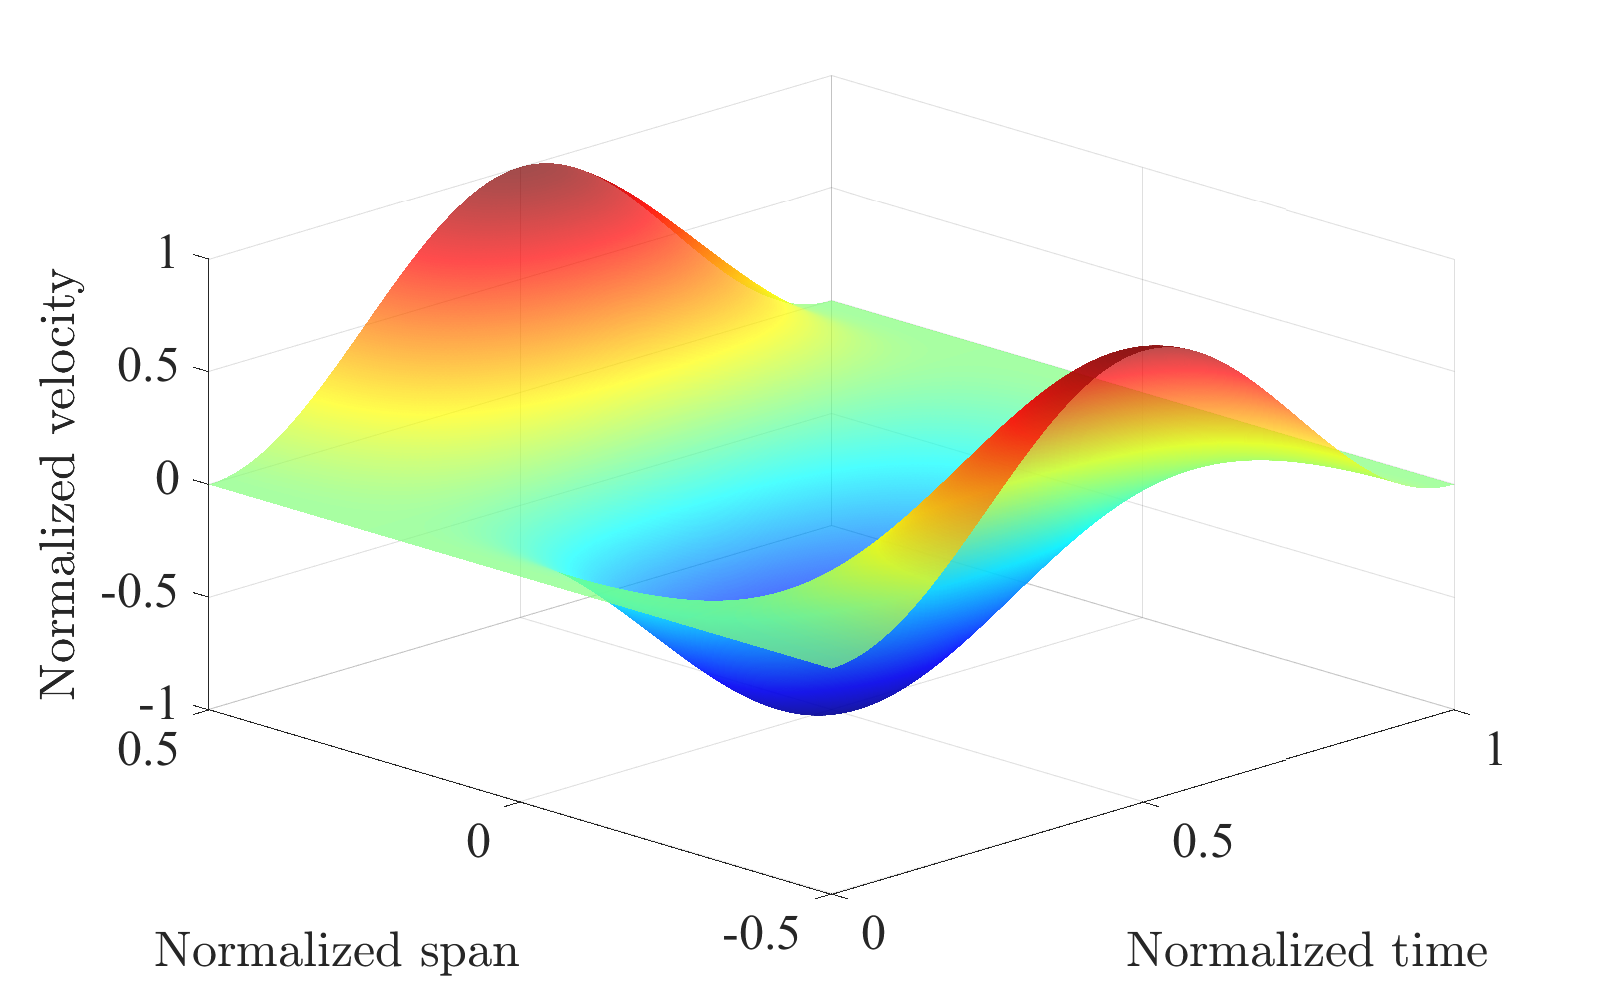
\includegraphics[width=0.7\linewidth,clip]{figures/DARPA_gust.pdf}	
    \label{fig:DARPA_gust}
    \legend{Source: the author.}
\end{figure}

\subsection{Continuous profiles: atmospheric turbulence}
\label{subsec:turb_model}

Atmospheric turbulence is modeled as a stationary Gaussian random process following the von Kármán spectrum. The Power Spectral Density (PSD) of the gust velocity in the longitudinal ($u$), lateral ($v$) and vertical ($w$) directions are given by \citeonline{hoblit1988gust} as
\begin{align}
    \Psi_{u}(\Omega) &= {\sigma}^2\frac{2L}{\pi}\frac{1}{[1+(1.339L\Omega)^2]^{5/6}} \ \ ,
    \\
    \Psi_{v}(\Omega) = \Psi_{w}(\Omega) &= {\sigma}^2\frac{L}{\pi}\frac{1+\frac{8}{3}(1.339L\Omega)^2}{[1+(1.339L\Omega)^2]^{11/6}} \ \ ,
    \label{eq:vkpsd_vw} 
\end{align}
where $\Omega$ is the spatial frequency argument, $\sigma$ is the root mean square (RMS) of the gust velocity and $L$ is the characteristic length scale of turbulence --- whose value of 2500 ft or 762 m is assumed here. 

There are two ways in which gust velocity profiles can be constructed in the time or spatial domains. The first is through the superposition of a large number of sinusoids with discrete frequencies, whose amplitudes are determined from the frequency content of the PSD. The gust velocity components obtained with this method are given in time as
\begin{align}
    u(t) &= \sum_{i} \sqrt{2\Psi_{u}(\Omega_i)\Delta\Omega} \cos\lp\Omega_i Ut+\varphi_i\rp \ \ ,
    \label{eq:ugvk_sinusoids}
    \\
    v(t) &= \sum_{i} \sqrt{2\Psi_{v}(\Omega_i)\Delta\Omega} \cos\lp\Omega_i Ut+\varphi_i\rp \ \ ,
    \label{eq:vgvk_sinusoids}
    \\
    w(t) &= \sum_{i} \sqrt{2\Psi_{w}(\Omega_i)\Delta\Omega} \cos\lp\Omega_i Ut+\varphi_i\rp \ \ ,
    \label{eq:wgvk_sinusoids} 
\end{align}
where $U$ is a reference airspeed, $\Delta\Omega = 2\pi U/T$ is the spatial frequency resolution, with $T$ being the time length of turbulence patch, $\Omega_i$ is the $i\textsuperscript{th}$ discrete frequency in the chosen range, and $0 \leq\varphi_i\leq2\pi$ is the corresponding random phase angle. This method is suitable if the airspeed is fixed and the gust duration predetermined, for instance, in a wind tunnel simulation setting.

The second method is through the ``coloring'' of a white noise signal with the turbulence filter, a process known as synthetic turbulence generation \cite{palacios2023dynamics}. This method can be used to define a gust field in space instead of time, making it suitable for simulations of aircraft in free flight. The 1-D idealization assumed means that the longitudinal, lateral and vertical gust velocities only vary in one direction, which is usually the ``forward flight'' one, i.e., $\uvec{\imath}_2$. In other words, the gust velocities are $u=u(x_2)$, $v=v(x_2)$ and $w=w(x_2)$, where $x_2$ is the coordinate in the direction of $\uvec{\imath}_2$, the second vector of the fixed inertial basis. Thus, if a gust field of length $\ell$ in the $x_2$ coordinate is discretized into $N$ nodes, then white noise (random) signals of length $N$, $u_n$, $v_n$, $w_n$ are generated, and the values of the gust velocity components at those nodes is obtained as
\begin{align}
     u(x_2) &= \mathbb{R}\lp\mathcal{F}^{-1}\lb\mathcal{F}[u_n]\sqrt{\Psi_u}\rb\rp \ \ ,
    \label{eq:uvk_whitenoise}
    \\
    v(x_2) &= \mathbb{R}\lp\mathcal{F}^{-1}\lb\mathcal{F}[v_n]\sqrt{\Psi_v}\rb\rp \ \ ,
    \label{eq:vvk_whitenoise}
    \\
    w(x_2) &= \mathbb{R}\lp\mathcal{F}^{-1}\lb\mathcal{F}[w_n]\sqrt{\Psi_w}\rb\rp \ \ ,
    \label{eq:wvk_whitenoise}
\end{align}
where $\mathbb{R}\lp\cdot\rp$ is the real part, $\mathcal{F}$ is the Fourier transform operator, and $\Psi_u$, $\Psi_v$, $\Psi_w$ are the PSDs for $0\leq\Omega\leq 2\pi N/\ell$. These gust velocities can be re-scaled to have the desired RMS, $\sigma$.

The resulting normalized vertical velocity PSDs, $\overline{\Psi}_w(\Omega)=\Psi_{w}(\Omega)/(\sigma^2L/\pi)$, obtained with both methods are illustrated in \cref{fig:vk_PSD}. The sinusoids superposition method yields almost perfect agreement with the definition of \cref{eq:vkpsd_vw}. The same cannot be said about the PSD curve with the white noise coloring method, which oscillates around the definition, but stays close to it. A smoothed curve (by moving average) is also provided for clarity.

\begin{figure}[hbt!]
    \centering	
    \caption{Normalized vertical velocity PSD, $\overline{\Psi}_w(\Omega)$.}
    \begin{subfigure}{0.49\textwidth}
	\centering
        \caption{Sinusoids superposition method.}
	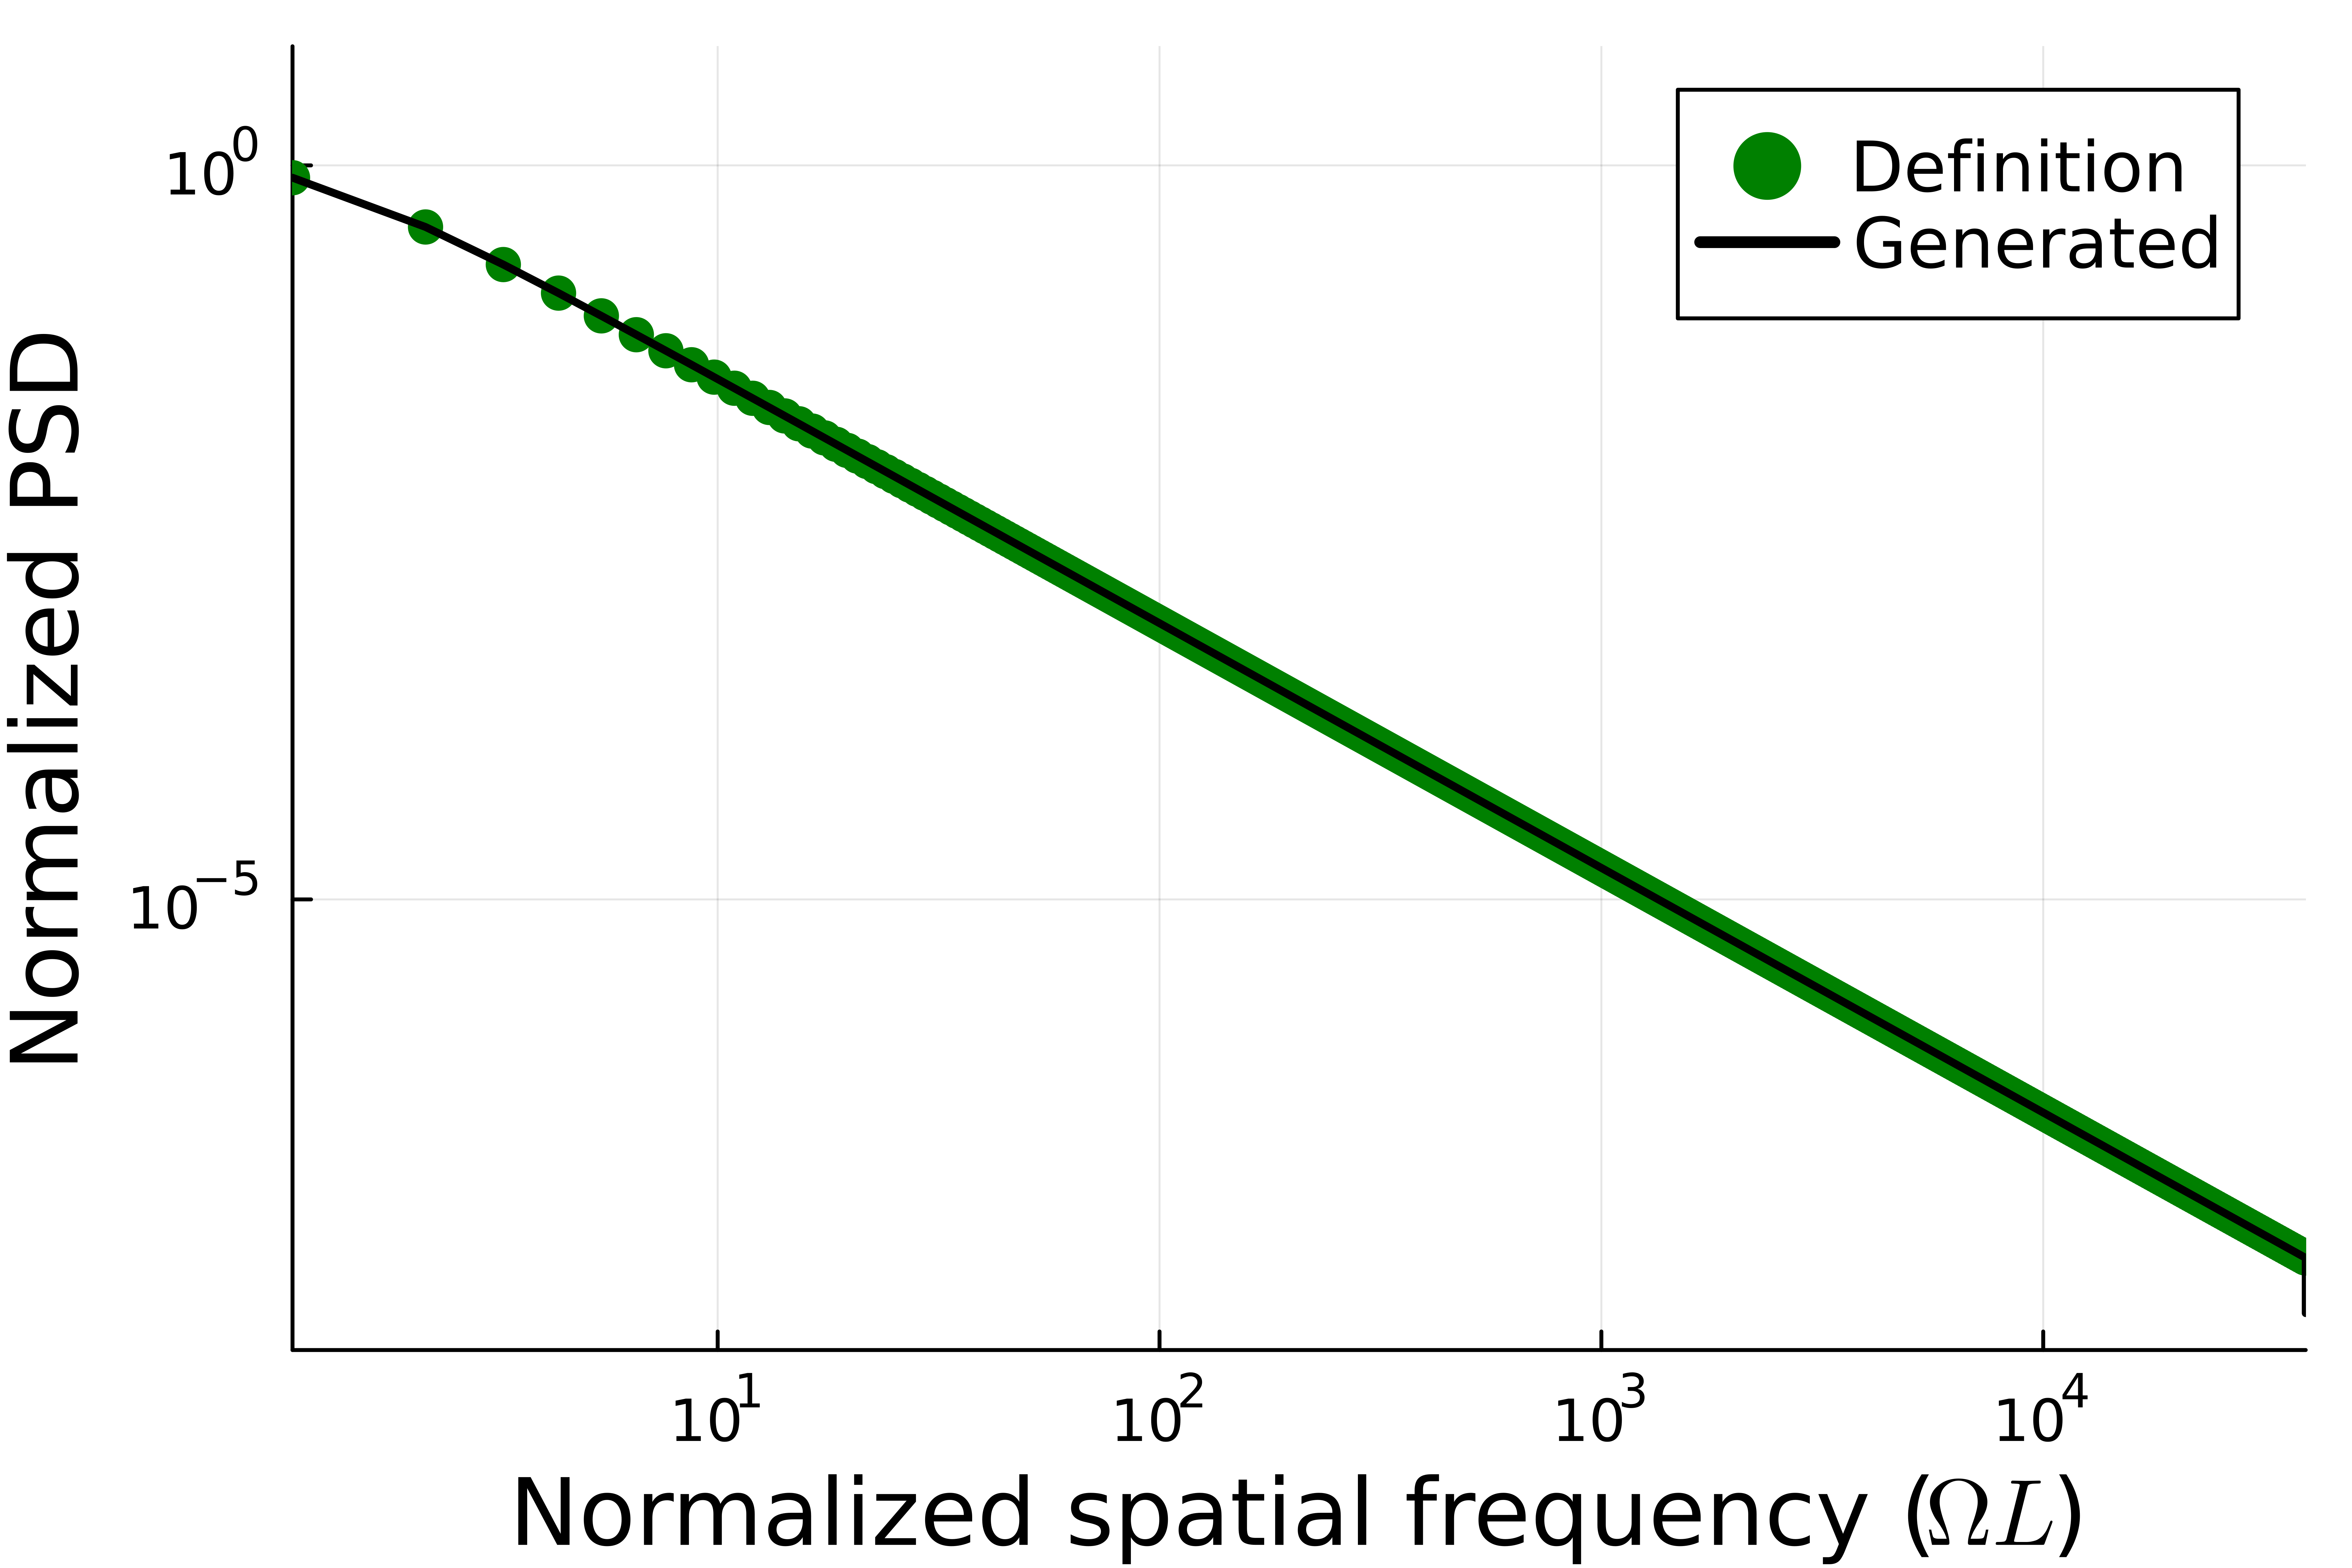
\includegraphics[width=1\linewidth, trim={0cm 0cm 0cm 0cm}, clip]{figures/PSD_sinusoids.png}
    \label{fig:vk_PSD_sinusoids}
    \end{subfigure}
    \begin{subfigure}{0.49\textwidth}
	\centering
        \caption{White noise coloring method.}
	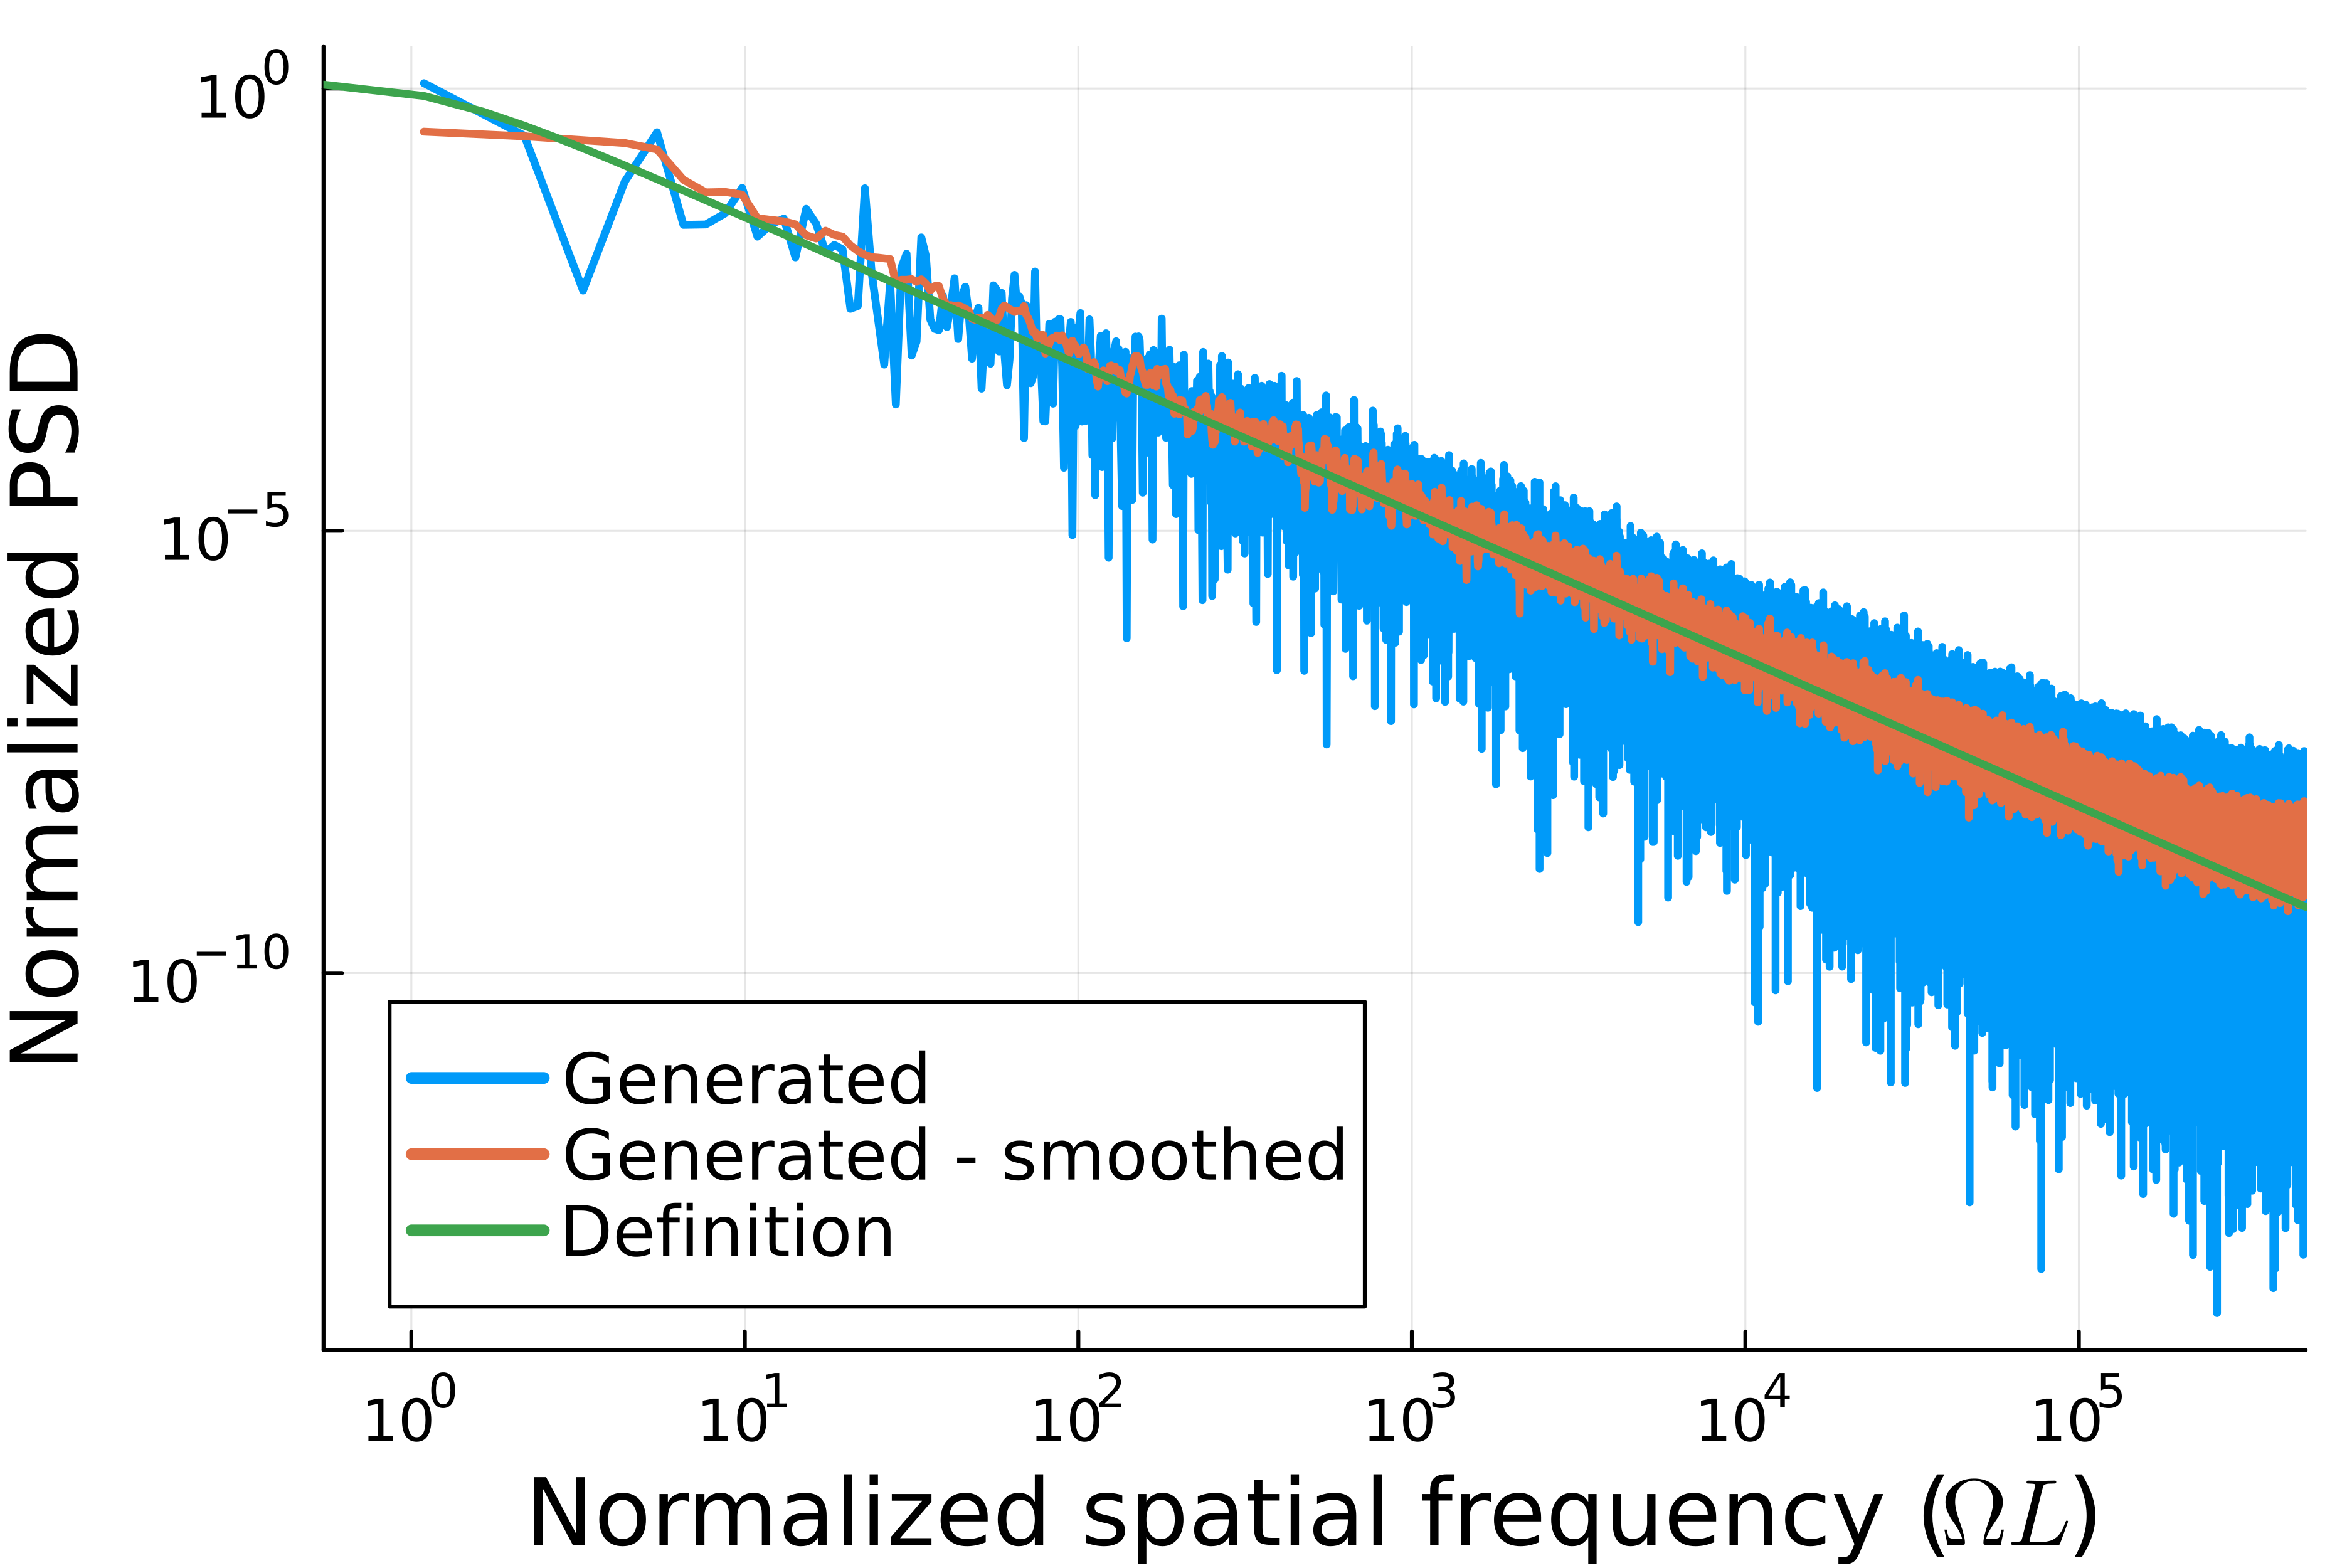
\includegraphics[width=1\linewidth, trim={0cm 0cm 0cm 0cm}, clip]{figures/PSD_whitenoise.png}
    \label{fig:vk_PSD_wnc}
    \end{subfigure}
    \label{fig:vk_PSD}
    \legend{Source: the author.}
\end{figure}

For the choice of the RMS of the gust velocity at low altitudes (below 2000 ft), the military standard MIL-STD-1797A \cite{milstd1797} suggests the use of
\begin{equation}
    \sigma = 0.1 u_{20}
    \label{eq:sigma_MIL_STD_1797}
\end{equation}
where $u_{20}$ is the mean wind speed at 20 ft altitude, whose probability of exceedance (per hour) is shown in \cref{fig:u20_MIL_STD_1797}.

\begin{figure}[hbt!]
    \centering
    \caption{Probability of exceeding mean wind speed at 20 ft altitude.}
    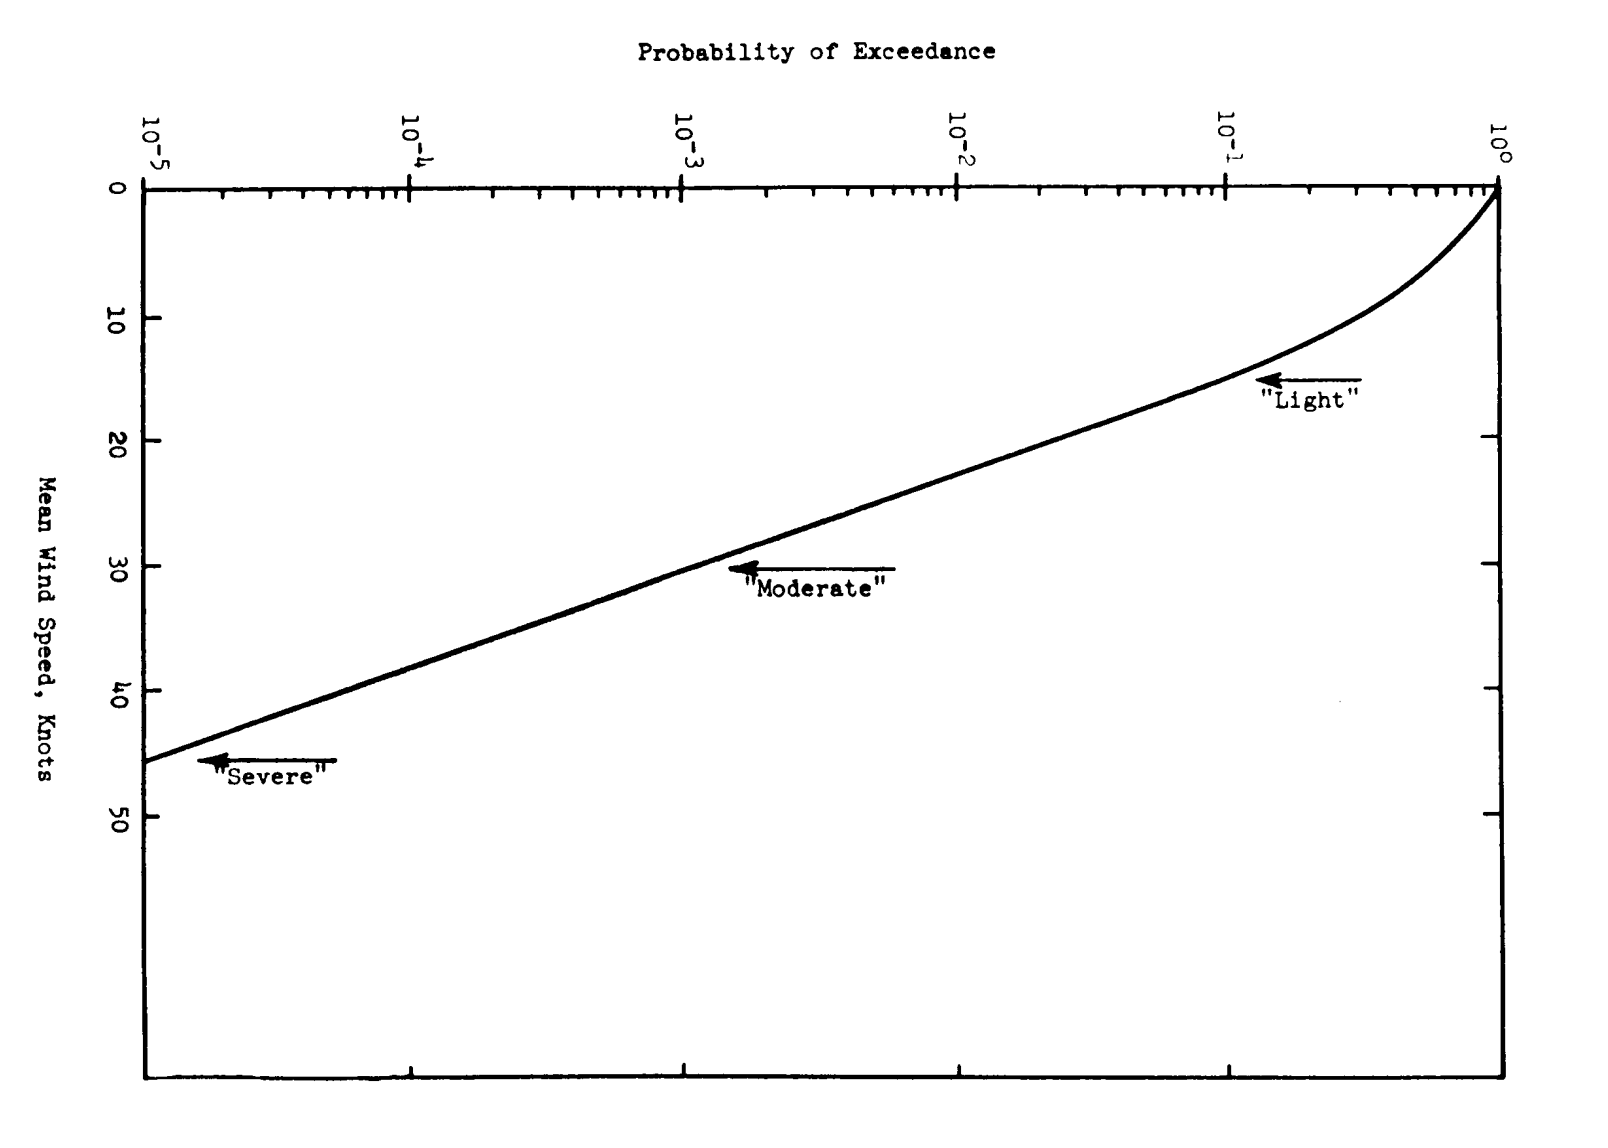
\includegraphics[width=0.8\linewidth,clip]{figures/u20_MIL_STD_1797.png}	
    \label{fig:u20_MIL_STD_1797}
    \legend{Source: \citeonline{milstd1797}}
\end{figure}

% Secion: Kinematical description in terms of beam variables
\section{Kinematical description in terms of beam variables}
\label{sec:kin_aero}

Until now, the aerodynamic kinematics have been described in terms of the variables from classical thin-airfoil theory: $U$ as the relative flow velocity magnitude, $\theta$ as the pitch angle, $\hdot$ as the plunge velocity, and $a$ and $d$ as the positions of the pitch axis and flap hinge, respectively. A description in terms of the kinematic variables (more specifically, the state variables) of the beam model is developed now.

Consider a local airfoil section belonging to an aerodynamic surface attached to a beam element of length $\Deltal$, as depicted in \cref{fig:airfoil_sec}. The unswept and untwisted airfoil section is assumed to be have a chord of length $c$, and to be initially attached to the beam such that it lies normal to the $\uvec{b}_1$ vector, and its chordline (running from point $T$, at the trailing-edge, to point $L$, at leading-edge) is aligned with the $\uvec{b}_2$ vector. An angle of sweep, $\Lambda$, and an angle of aerodynamic twist (wash-out or wash-in), $\phi$, rotate this section about axes $\uvec{b}_3$ and $\uvec{b}_1$, respectively. The basis obtained by such rotations is called the \textit{undeformed beam aerodynamic basis} $\wt(\xo,t) = [\uvec{w}_1(\xo,t),\uvec{w}_2(\xo,t),\uvec{w}_3(\xo,t)]$. The components of the rotation tensor that bring the undeformed beam basis $\bp$ to the undeformed beam aerodynamic basis $\wt$, resolved in basis $\A$, are denoted $\Rw$. Note that following the transformation rule for second-order tensors, $\Rw=\Rz\Rw^+\RzT$, where $\Rw^+$ is $\Rw$ resolved in basis $\bp$, where it is most naturally described in terms of $\Lambda$ and $\phi$. A generalized point $P$ in the chordline is such that its chord-normalized position with respect to point $L$ is $s_P$. Point $b$, at the origin of the $\bp$ and $\wt$ bases, is called the \textit{attachment point}. It defines the local position of the beam's reference line, and is assumed to be crossed by the airfoil's chordline. The chord-normalized position of point $b$ with respect to point $L$, denoted $s$, is thus sufficient to define the position of the airfoil section with respect to the beam. Of course, the small strains assumption implies that $s$, $s_P$ and any other distances between points in the airfoil, remain constant upon deformation. Note that upon being swept, the length of the chord is assumed to become $c\sec\Lambda$, which is the value used to compute aerodynamic load resultants (see \cref{eq:f_a,eq:m_a}.

\begin{figure}[ht!]
    \centering
    \caption{Swept and twisted airfoil section attached to a beam element.}		
    \begin{subfigure}{0.7\textwidth}
        \centering
        \caption{Side view (before being swept).}
	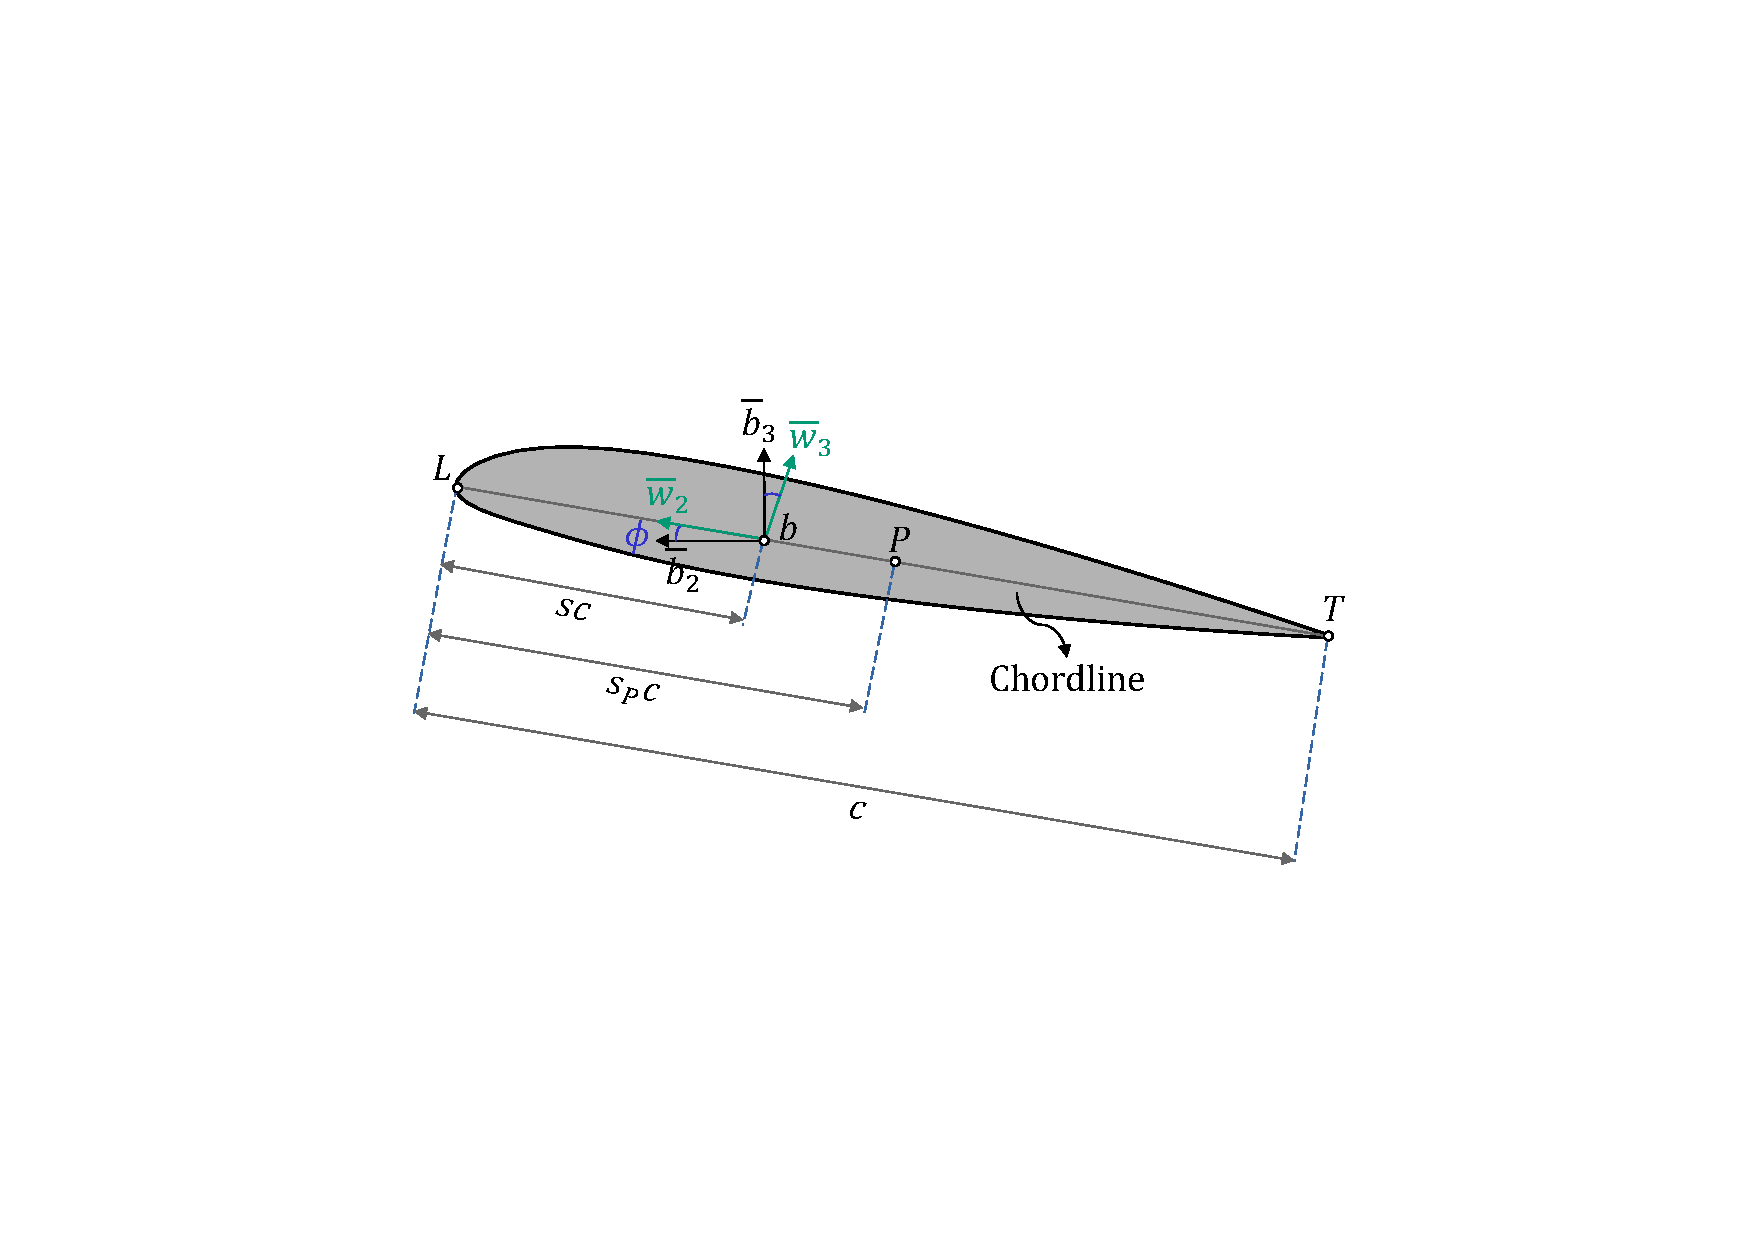
\includegraphics[width=1.0\linewidth,trim={6cm 6.3cm 6cm 6.5cm}, clip]{figures/aero_section_side.pdf}
        \label{fig:airfoil_sec_sideview}
    \end{subfigure}
    \begin{subfigure}{0.7\textwidth}
        \centering
        \caption{Top view.}
	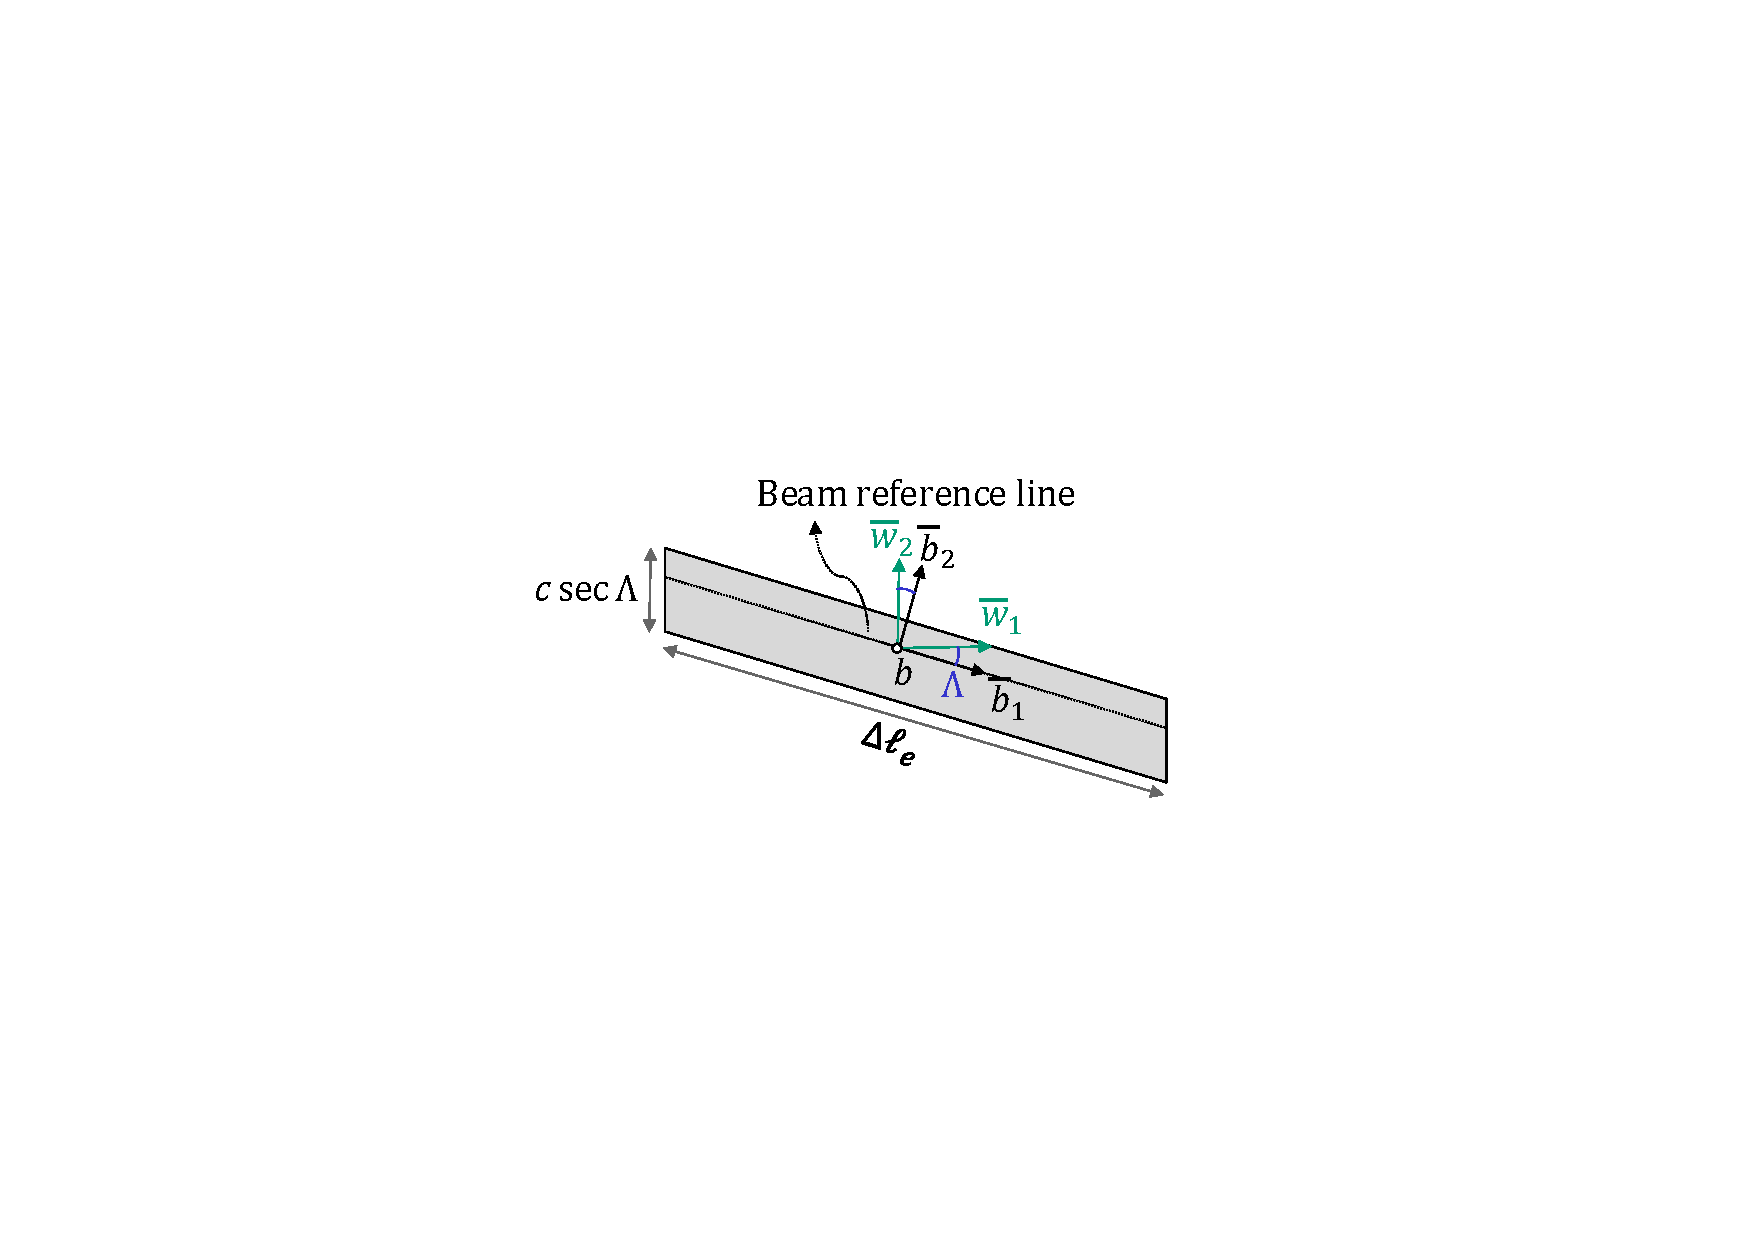
\includegraphics[width=1.0\linewidth,trim={9cm 7.5cm 9cm 7.5cm}, clip]{figures/aero_section_top.pdf}
        \label{fig:airfoil_sec_topview}
    \end{subfigure}
    \label{fig:airfoil_sec}
    \legend{Source: the author.}
\end{figure}

The \textit{deformed beam aerodynamic basis}, $\scalebox{0.9}{$\displaystyle \Ws(\xo,t) = [\uvec{W}_1(\xo,t),\allowbreak\ \uvec{W}_2(\xo,t),\allowbreak\ \uvec{W}_3(\xo,t)]$}$ , results from the undeformed one, $\wt$, being rotated by the deformation rotation tensor, $\R$. Thus, any vector $\vect{v}$, resolved in basis $\Ws$, is written in terms of the components resolved in basis $\B*$ through the transformation rule as
\begin{align}
    \vect{v}^\square &= \RT\vect{v}^\triangle \nonumber 
    \\
    &= \lp\R\;\Rw\rp^\T\vect{v}^+ \nonumber 
    \\
    &= \RwT\RT\vect{v}^+ \nonumber 
    \\ 
    &= \RwT\vect{v}^* \ \ .
    \label{eq:vstar_to_vsquare} 
\end{align}

Then, the \textit{local relative wind velocity vector} ``seen'' by the airfoil at the attachment point, is simply the negative of the beam's inertial sectional velocity vector \cite{drela2014flight}, resolved in the deformed beam aerodynamic basis $\Ws$,
\begin{align}
    \Us = \{U_1,U_2,U_3\}^\T = -\RwT\Vs \ \ ,
    \label{eq:Us} 
\end{align}
where $U_1$, $U_2$, and $U_3$ are respectively denoted the spanwise, tangential, and normal wind velocity components. The normal components of the relative wind velocity and acceleration vector may be constructed at any point $P$ along the airfoil's chordline by respectively adding to $\Us$ and $\Usdot$, components due to the inertial sectional angular velocity and acceleration of the beam resolved in basis $\Ws$, yielding
\begin{align}
    \Usp &= \Us - \Omtilsq\vect{\xi}_P^{\square}
    \ \ , \label{eq:Usp}
    \\
    \Uspdot &= \Usdot - \Omtilsqdot\vect{\xi}_P^{\square} \ \ ,
    \label{eq:Uspdot}
\end{align}
in which $\vect{\xi}_P^{\square} = c\{0,s-s_P,0\}^\T$ is the position vector between points $P$ and $b$. The normal components of $\Usp$ and $\Uspdot$ are the ones in the direction of $\uvec{W}_3$, which may be written as
\begin{align}
    U_{P_3} &= U_{3} - \Omega_1^{\square} c \lp s-s_P \rp \ \ ,
    \label{eq:Usp3}
    \\
    \dot{U}_{P_3} &= \dot{U}_{3} - \dot{\Omega}_1^{\square} c \lp s-s_P \rp \ \ .
    \label{eq:Uspdot3}
\end{align}

With all necessary definitions in place, it is possible to begin extracting equivalences. Foremost, the assumption of two-dimensional flow from strip theory indicates that the magnitude of the relative wind velocity from thin-airfoil theory is equivalent to the in-plane wind velocity, that is,
\begin{equation}
    U \equiv \Uip \coloneqq \sqrt{U_2^2+U_3^2} \ \ .
    \label{eq:U_equiv}
\end{equation}

The pitch rate is equivalent to the first component of the angular velocity vector resolved in the $\Ws$ basis,
\begin{equation}
    \thetadot \equiv \Omega_1^{\square} \ \ .
    \label{eq:thetadot_equv}
\end{equation}

Also, the deflection angle of the trailing-edge flap, $\delta_f$, clearly has a direct equivalence, and a simple expression arises from geometric arguments to write the positions of the attachment point and flap hinge as
\begin{align}
    a &\equiv 2s-1 \ \ ,
    \label{eq:a_equiv}
    \\
    d &\equiv 2s_f-1 \ \ ,
    \label{eq:d_equiv}
\end{align}
in which $s_f$ is the chord-normalized position of the flap hinge. These simple equivalences are in contrast with those for the pitch angle and plunge velocity. For instance, the definition of the quasi-steady angle of attack at the pitch axis (attachment point) indicates the following equivalences
\begin{align}
    U\cos\theta - \hdot\sin\theta &= v_{pp}^{QS} \equiv -U_2 \ \ ,
    \label{eq:w_pp_equiv}
    \\
    U\sin\theta + \hdot\cos\theta &= w_{pp}^{QS} \equiv U_3 \ \ .
    \label{eq:v_pp_equiv}
\end{align}

Furthermore, the beam with the airfoil section attached depicted in \cref{fig:airfoil_sec} may be enclosed in a time-dependent gust field whose known current local inertial velocity vector components at the attachment point, resolved in basis $\Io$, are $\Ugo$. The components of this vector resolved in the deformed beam aerodynamic basis are therefore given by 
\begin{align}
    \Ugsq &= \lp\Ro\Rwo\Rzo\RAo\rp^\T\Ugo
    \nonumber 
    \\
    &= \lb\lp\RAo\R\;\RAoT\rp\lp\RAo\Rw\RAoT\rp\;\lp\RAo\Rz\RAoT\rp\RAo\rb^\T\Ugo 
    \nonumber 
    \\
    &= \lp\RA\R\;\Rw\;\Rz\rp^\T\Ugo  
    \nonumber 
    \\
    &= \RRwRzT\RAT\Ugo
    \label{eq:Ugs} 
    \\
    &=\{U_{g_1},U_{g_2},U_{g_3}\}^\T \ \ ,
\end{align}
so that the quasi-steady tangential and normal velocity components of the gust are, respectively,
\begin{align}
    v_g^{QS} &\equiv -U_{g_2} \ \ ,
    \label{eq:vg_equiv}
    \\
    w_g^{QS} &\equiv U_{g_3} \ \ .
    \label{eq:wg_equiv}
\end{align}

By specifying the gust field and keeping track of the position, orientation, and velocities of each element of the beam assembly, it is thus possible to determine the local gust velocity components.

From the fundamental equivalences in \cref{eq:U_equiv,eq:thetadot_equv,eq:a_equiv,eq:d_equiv,eq:w_pp_equiv,eq:v_pp_equiv,eq:wg_equiv,eq:vg_equiv}, all of the previous aerodynamic equations can be described in terms of state variables of the beam model. 

% Section: Aeroelastic coupling
\section{Aeroelastic coupling}
\label{sec:aero_coupling}

As shown in \cref{sec:kin_aero}, the deformed beam velocity states, $\Vs$ and $\Oms$, are the ones involved in the calculation of aerodynamic loads. Since they are constant (along the span of an element, not over space and time), elemental variables in the finite element model implementation, the simplest approach with respect to coupling of the aerodynamic and structural models is to calculate the aerodynamic loads on an elemental basis as well. This means that each element is assumed to have one aerodynamic strip associated to it, and no interpolation is necessary for the transfer of generalized loads and displacements between the aerodynamic and structural meshes. In other words, each beam element with an associated aerodynamic strip develops its own unique aerodynamic load array, which is distributed over that element's nodes according to the methodology discussed in \cref{sec:3D_aero}.

Therefore, the aerodynamic state equations for each element (with an attached aerodynamic surface) can be grouped and written in the standard first-order form as
\begin{align}
    \aerostatesrates = \tens{A}_a \aerostates + \vect{B}_a \ \ ,
    \label{eq:aero_system}
\end{align}
in which $\vect{\chi}_a$ is the array of elemental aerodynamic state variables, $\tens{A}_a$ is the aerodynamic state matrix, and $\vect{B}_a$ is the aerodynamic input array, which may take different forms depending on the aerodynamic theory employed. The system of \cref{eq:aero_system} is seamlessly appended to the beam model's system of equations in \cref{eq:system} to produce a complete aeroelastic system, and the respective aerodynamic contributions to the residual, Jacobian, and inertia matrices are described in \cref{appendix_fem}.


%%%%%%%%%%%%%%%%%%%%%%%%%%%%%%%%%%%%%%%%%%%%%%%%%%%%%%%%%%%%%%%%%%%%%%%%%%%%%%%%%%%%%%%%%%%%%%%%%%%%%%%%%%%%%%%%%%%%%%%%%%%%%%%%%%%%%%%%%%%%%%%%%%%%%%%%%%%%%%%%
%%%%%%%%%%%%%%%%%%%%%%%%%%%%%%%%%% APPENDICES %%%%%%%%%%%%%%%%%%%%%%%%%%%%%%%%%%
%%%%%%%%%%%%%%%%%%%%%%%%%%%%%%%%%%%%%%%%%%%%%%%%%%%%%%%%%%%%%%%%%%%%%%%%%%%%%%%%%%%%%%%%%%%%%%%%%%%%%%%%%%%%%%%%%%%%%%%%%%%%%%%%%%%%%%%%%%%%%%%%%%%%%%%%%%%%%%%%
\begin{apendicesenv}

    \chapter{Intrinsic equations of motion}
\label{appendix_ieom}

To derive the \textit{intrinsic form} of the equations of motion, that is, a form that is independent of displacement and rotation variables, the variations of the generalized sectional strains and velocities must be expressed in terms of the variations of such displacement and rotation variables.

\section{Variation of sectional strains and strain energy}
\label{sec:str_U}

To express the variation of rotation variables, it is necessary to introduce the \textit{virtual rotation vector}, whose components in the deformed beam basis are defined analogously to those of an angular velocity vector as
\begin{align}
    \delpsis \coloneqq  \axial\lp\RpT\delta\Rp\rp \ \ ,
    \label{eq:del_psis}
\end{align}
where the extended underline notation, $\delpsis$, with an underline extending under the variational operator, is used instead of $\delta\vect{\psi}^*$, to emphasize that the virtual rotation vector is not the variation of a function, i.e., there exists no ``rotation vector'', $\vect{\psi}^*$, such that $\delpsis = \delta\lp\vect{\psi}^*\rp$ \cite{bauchau2011flexible}. The components of the vector product operator of the virtual rotation vector, resolved in basis $\B*$, are, by definition,
\begin{align}
    \delpsitils &\coloneqq  \RpT\delta\Rp \nonumber 
    \\
    &= \lp\delta\RpT\Rp\rp^T 
    \nonumber 
    \\
    &= -\delta\RpT\Rp \ \ ,
    \label{eq:del_psitils}
\end{align}
from which the variation of rotation tensors $\RpT$ and $\Rp$ may be found as
\begin{align}
    \delta\RpT &= -\delpsitils\RpT \ \ , \label{eq:del_RpT} 
    \\
    \delta\Rp &= \Rp\delpsitils \ \ ,
    \label{eq:del_Rp}
\end{align}

Taking a derivative with respect to $\xo$ of \cref{eq:del_psitils} yields
\begin{align}
    \delpsitilps &=  -\lp\delta\RpT\Rp\rp^\prime \nonumber 
    \\
    &= -\delta\RpprimeT\Rp - \delta\RpT\Rpprime \ \ ,
    \label{eq:del_psitilps}
\end{align}
and therefore,
\begin{align}
    -\delta\RpprimeT\Rp &= \delpsitilps + \delta\RpT\Rpprime \ \ .
    \label{eq:del_RpprimeTRp}
\end{align}

Furthermore, $\RpprimeT$ may be isolated in \cref{eq:Ktils} to yield
\begin{align}
    \RpprimeT &= \RpT\ktilp\Rp\RpT - \Ktils\RpT
    \nonumber 
    \\
    &= \RpT\ktilp - \Ktils\RpT \ \ ,\label{eq:RpprimeT} 
\end{align}
and thus,
\begin{align}
    \Rpprime &= \Rp\Ktils - \ktilp\Rp \ \ .
    \label{eq:Rpprime}
\end{align}

The variation of the moment-strains' vector product operator can be obtained starting from \cref{eq:Ktils} and using Eqs.~\eqref{eq:del_RpT}, \eqref{eq:del_Rp}, \eqref{eq:del_RpprimeTRp}, \eqref{eq:RpprimeT}, and \eqref{eq:Rpprime} to find
\begin{align}
    \delta\kapptil =& \;\delta\Ktils - \cancelto{0}{\delta\ktilp} \nonumber 
    \\
    =& \;\delta\lp-\RpprimeT\Rp + \RpT\ktilp\Rp\rp \nonumber 
    \\
    =& -\delta\RpprimeT\Rp - \RpprimeT\delta\Rp + \delta\RpT\ktilp\Rp + \RpT\cancelto{0}{\delta\ktilp}\Rp + \RpT\ktilp\delta\Rp
    \nonumber 
    \\
    =& -\delta\RpprimeT\Rp - \RpprimeT\delta\Rp + \delta\RpT\ktilp\Rp + \RpT\ktilp\delta\Rp \nonumber 
    \\
    =& \lb\delpsitilps + \lp-\delpsitils\RpT\rp \lp\Rp\Ktils - \ktilp\Rp\rp\rb - \lb\lp\RpT\ktilp - \Ktils\RpT\rp\lp\Rp\delpsitils\rp\rb + \nonumber 
    \\ 
    & \lb\lp-\delpsitils\RpT\rp\ktilp\Rp\rb + \lb\RpT\ktilp\lp\Rp\delpsitils\rp\rb \nonumber 
    \\
    =& \;\delpsitilps - \delpsitils\RpT\lp\Rp\Ktils - \ktilp\Rp\rp - \RpT\ktilp\Rp\delpsitils + \Ktils\RpT\Rp\delpsitils + \nonumber 
    \\ 
    & -\delpsitils\RpT\ktilp\Rp + \RpT\ktilp\Rp\delpsitils \nonumber 
    \\
    =& \;\delpsitilps - \delpsitils\Ktils + \delpsitils\RpT\ktilp\Rp - \RpT\ktilp\Rp\delpsitils + \Ktils\delpsitils + \nonumber 
    \\ 
    & -\delpsitils\RpT\ktilp\Rp + \RpT\ktilp\Rp\delpsitils \nonumber 
    \\
    =& \;\delpsitilps + \Ktils\delpsitils - \delpsitils\Ktils \ \ ,
    \label{eq:del_kappa_p_til}
\end{align}
where the fact that $\delta\ktilp = \delta\lp\RzT\Rzp\rp = \delta\RzT\Rzp + \RzT\delta\Rzp = \zthree + \zthree = \zthree$ was used, because basis $\bp$ is fixed with respect to basis $\A$, and so there are no kinematically admissible variations for $\Rz$ and its derivatives in basis $\A$. Applying the property that $\til{a}\til{b}-\til{b}\til{a} = \til{\lp\til{a}\vect{b}\rp}$, for any $\vect{a}$ and $\vect{b}$, one may write $\Ktils\delpsitils - \delpsitils\Ktils = \til{\lp\Ktils\delpsis\rp}$, so that \cref{eq:del_kappa_p_til} then implies
\begin{align}
    \delta\kapp &= \delpsips + \Ktils\delpsis \ \ ,
    \label{eq:del_kappa_p} 
\end{align}
and finally,
\begin{align}
    \delta\kappT &= \delpsipsT - \delpsisT\Ktils \ \ .
    \label{eq:del_kappa_pT}
\end{align}

To achieve more compact expressions associated with the variation of the displacement, the \textit{virtual displacement vector} is introduced, whose components resolved in bases $\bp$, $\B*$, and $\A$, are respectively defined as
\begin{align}
    \delqp &\coloneqq \delta\uplus \ \ ,
    \label{eq:delqp} 
    \\
    \delqs &\coloneqq \RpT\delta\uplus  = \RpT\delqp \ \ ,
    \label{eq:delqs}	
    \\
    \delq &\coloneqq \Rz\delta\uplus = \Rz\delqp = \Rz\Rp\delqs \ \ ,
    \label{eq:delq}
\end{align}
where it can be noticed that whereas the extended underline notation could be dropped on $\delqp$, since it is the variation of $\uplus$, it cannot be dropped on $\delqs$ and $\delq$, because these cannot be written as the variation of a function. Equation \eqref{eq:delqs} implies that 
\begin{align}
    \delta\uplus = \Rp\delqs \ \ ,
    \label{eq:deluplus}
\end{align}
whose derivative for $\xo$ yields 
\begin{align}
    \delta\upprime = \Rpprime\delqs + \Rp\delqps \ \ ,
    \label{eq:delupprime}
\end{align}
and therefore,
\begin{align}
    \RpT\delta\upprime &= \RpT\Rpprime\delqs + \RpT\Rp\delqps \nonumber 
    \\
    &= \delqps - \RpprimeT\Rp\delqs \ \ ,
    \label{eq:RpTdelupprime}
\end{align}
where the knowledge that $\RpT\Rpprime$ is skew-symmetric was used to write 
\begin{align}
\RpT\Rpprime = -\lp\RpT\Rpprime\rp^T = -\RpprimeT\Rp \ \ . 
\end{align}

Additionally, \cref{eq:gamp_b} may be rearranged as
\begin{align}
    \lp\aone+\upprime+\ktilp\uprime\rp = \Rp\lp\aone+\gamp\rp \ \ .
    \label{eq:gamp_b_rearranged}
\end{align}

The variation of the force-strains vector can now be achieved starting from \cref{eq:gamp_b} and using Eqs.~\eqref{eq:del_psitils}, \eqref{eq:RpprimeT}, \eqref{eq:deluplus}, \eqref{eq:RpTdelupprime}, and \eqref{eq:gamp_b_rearranged} to find
\begin{align}
    \delta\gamp &= \delta\lb\RpT\lp\aone + \upprime + \ktilp\uplus\rp - \aone\rb \nonumber 
    \\
    &= \delta\RpT\lp\aone+\upprime+\ktilp\uplus\rp + \RpT\lp\delta\upprime + \ktilp\delta\uplus+ \cancelto{\zv}{\delta\ktilp}\uplus\rp \nonumber 
    \\
    &= \delta\RpT\lb\Rp\lp\aone+\gamp\rp\rb + \RpT\delta\upprime + \RpT\ktilp\delta\uplus \ \ , \label{eq:delgamp_analogy} 
    \\
    &= \delpsitilsT\lp\aone+\gamp\rp + \lp\delqps - \RpprimeT\Rp\delqs\rp + \RpT\ktilp\lp\Rp\delqs\rp \nonumber 
    \\
    &= \lp\aonetil+\gamptil\rp\delpsis + \delqps - \lp\RpT\ktilp - \Ktils\RpT\rp\Rp\delqs + \RpT\ktilp\Rp\delqs \nonumber 
    \\
    &= \delqps + \Ktils\delqs + \lp\aonetil+\gamptil\rp\delpsis  \ \ ,
    \label{eq:delgamp}
\end{align}
where the property that $\til{a}^T\vect{b} = \til{b}\vect{a}$, for any $\vect{a}$ and $\vect{b}$, was used to write 
\begin{align}
\delpsitilsT\lp\aone+\gamp\rp = \lp\aonetil+\gamptil\rp\delpsis \ \ , 
\end{align}
and finally, it is also used in writing
\begin{align}
    \delta\gampT &= \lb\delqps + \Ktils\delqs + \lp\aonetil+\gamptil\rp\delpsis\rb^T \nonumber 
    \\
    &= \delqpsT + \delqsT\KtilsT + \delpsisT\lp\aonetil+\gamptil\rp^T \nonumber 
    \\
    &= \delqpsT - \delqsT\Ktils - \delpsisT\lp\aonetil+\gamptil\rp \ \ .
    \label{eq:delgampT}
\end{align}

Substituting Eqs.~\eqref{eq:del_kappa_pT} and \eqref{eq:delgampT} into \cref{eq:delU} yields a final expression for the variation of the strain energy in terms of the virtual displacement and virtual rotation vectors,
\begin{align}
    \delta\mathcal{U} &= \lb\delqpsT - \delqsT\Ktils - \delpsisT\lp\aonetil+\gamptil\rp\rb\Fs + \lb\delpsipsT - \delpsisT\Ktils\rb\Ms \ \ .
    \label{eq:delU_final}
\end{align}

\section{Variation of sectional velocities and kinetic energy}
\label{sec:vel_K}

The variations of the sectional generalized velocities remain to be found. Taking a variation of \cref{eq:Omegatil_star} yields
\begin{align}
    \delta\Omtils &= \delta\lp -\RpTdot\Rp + \RpT\omtilp\Rp \rp \nonumber 
    \\
    &= -\delta\RpTdot\Rp - \RpTdot\delta\Rp + \delta\RpT\omtilp\Rp + \RpT\cancelto{\zthree}{\delta\omtilp}\Rp + \RpT\omtilp\delta\Rp \nonumber 
    \\
    &= -\delta\RpTdot\Rp - \RpTdot\delta\Rp + \delta\RpT\omtilp\Rp + \RpT\omtilp\delta\Rp \ \ ,
    \label{eq:del_Omegatil_star}
\end{align}
where $\delta\omtilp = \zthree$ stems from the fact that the motion of basis $\A$ is assumed to be known at all instants in time. Were this hypothesis to be relaxed, this term would be carried out in the developments and would later yield additional equations governing the angular velocity of basis $\A$ with respect to the inertial basis.

Since the variations of the generalized sectional velocities are to be expressed in terms of the virtual displacement and rotation vectors, just like in the case of the generalized strains, suitable expressions for the terms in the right-hand side of \cref{eq:del_Omegatil_star} must be found. Fortunately, there is an analogy between the angular velocities ($\Oms$ and $\omp$) and the curvatures ($\Ks$ and $\kp$) in the development of their variations. Because $\delta\kapptil = \delta\Ktils$, and $\delta\Omtils$ and $\omtilp$ in \cref{eq:del_Omegatil_star} are analogous to $\delta\Ktils$ and $\ktilp$ in \cref{eq:del_kappa_p_til}, it follows that $\delta\OmsT$ can be obtained from \cref{eq:del_kappa_pT} by simply replacing $\kapp$ and $\Ks$ by $\Oms$, and exchanging the spatial derivatives by time derivatives, that is,
\begin{align}
    \delta\OmsT &= \delpsisdotT - \delpsisT\Omtils \ \ .
    \label{eq:del_OmsT}
\end{align}

Proceeding similarly for the sectional velocity, a variation of \cref{eq:V_star} is taken to yield
\begin{align}
    \delta\Vs &= \delta\lb \RpT \lp\vbplus + \omtilp\uplus + \updot\rp \rb \nonumber 
    \\
    &= \delta\RpT\lp\vbplus + \omtilp\uplus + \updot\rp + \RpT\lp\cancelto{\zv}{\delta\vbplus} + \cancelto{\zthree}{\delta\ktilp}\uplus + \omtilp\delta\uplus + \delta\updot\rp \nonumber 
    \\
    &= \delta\RpT\Rp\Vs + \RpT\omtilp\delta\uplus + \RpT\delta\updot \ \ ,
    \label{eq:del_V_star}
\end{align}
where $\delta\vbplus = \vect{0}$ for the same reason that $\delta\omtilp = \zthree$, and were the movement of basis $\A$ to be unknown, it would be carried and would later provide additional equations governing the velocity of basis $\A$ in basis $\Io$. 

Comparing Eqs.~\eqref{eq:del_V_star} and \eqref{eq:delgamp_analogy}, it is clear that
there is an analogy between the variation of the sectional velocity, $\delta\Vs$, and that of the force-strains, $\delta\gamp$. This observation, which the reader may verify by performing the calculations, indicates that $\delta\VsT$ may be directly obtained from \cref{eq:delgampT}, by replacing $\gamp$ by $\Vs$, $\Ktils$ by $\Omtils$, $\lp\aonetil+\gamptil\rp$ by $\Vtils$, and the spatial derivatives by time derivatives, yielding,
\begin{align}
    \delta\VsT &= \delqdotsT - \delqsT\Omtils - \delpsisT\Vtils \ \ .
    \label{eq:delVsT}
\end{align}

Finally, with Eqs.~\eqref{eq:del_OmsT} and \eqref{eq:delVsT} at hand, it is possible to recast the expression for the variation of the kinetic energy from \cref{eq:delK} as
\begin{align}
    \delta\mathcal{K} &= \lb\delqdotsT - \delqsT\Omtils - \delpsisT\Vtils\rb\Ps + \lb\delpsisdotT - \delpsisT\Omtils\rb\Hvs \ \ .
    \label{eq:delK_final}
\end{align}

\section{Intrinsic equations}
\label{sec:intrinsic_eq}

Using Eqs.~\eqref{eq:delU_final} and \eqref{eq:delK_final}, and introducing the expressions for the virtual work and virtual action in Eqs.~\eqref{eq:deltaA} and \eqref{eq:deltaWs}, Hamilton's principle, stated in \cref{eq:hamilton}, resumes to
\begin{align}
    \intt\intl \Biggl\{\Biggr.&
    \delqsT\fs + \delpsisT\ms + \lb\delqdotsT - \delqsT\Omtils - \delpsisT\Vtils\rb\Ps + \lb\delpsisdotT - \delpsisT\Omtils\rb\Hvs + 
    \nonumber 
    \\
    &-\lb\delqpsT - \delqsT\Ktils - \delpsisT\lp\aonetil+\gamptil\rp\rb\Fs - \lb\delpsipsT - \delpsisT\Ktils\rb\Ms  \Biggl.\Biggr\} \;\d\xo\;\d t \nonumber \\
    &= \intl\lp \delqsT\Phats + \delpsisT\Hhats \rp\Big|_{t_1}^{t_2} \; \d \xo - \intt\lp  \delqsT\Fhats + \delpsisT\Mhats \rp\Big|_{0}^{l} \; \d t \ \ .
    \label{eq:hamilton_expanded}
\end{align}

Now, consider the following integrations by parts,
\begin{equation}
\begin{aligned}
    \intt\intl \delqdotsT\Ps \;\d\xo\;\d t &= \intl \lp \delqsT\Ps \rp\Big|_{0}^{l} \;\d\xo - \intt\intl \delqsT\Pdots \;\d\xo\;\d t \ \ , 
    \nonumber 
    \\
    \intt\intl \delpsisdotT\Hvs \;\d\xo\;\d t &= \intl \lp \delpsisT\Hvs \rp\Big|_{0}^{l} \;\d\xo - \intt\intl \delpsisT\Hvdots \;\d\xo\;\d t \ \ , 
    \nonumber 
    \\
    \intl\intt \delqpsT\Fs \;\d t\;\d\xo &= \intt \lp \delqsT\Fs \rp\Big|_{t_1}^{t_2} \;\d t - \intl\intt \delqsT\Fsprime \;\d t\;\d\xo \ \ , 
    \nonumber 
    \\
    \intl\intt \delpsipsT\Ms \;\d\xo\;\d t &= \intt \lp \delpsisT\Ms \rp\Big|_{t_1}^{t_2} \;\d t - \intl\intt \delpsisT\Msprime \;\d t\;\d\xo \ \ .
    \label{eq:int_parts}
\end{aligned}
\end{equation}

Substituting these expressions into \cref{eq:hamilton_expanded} and collecting terms leads to
\begin{equation}
\begin{aligned}
    \intt\intl \Biggl\{\Biggr.&
    \hphantom{+}\delqsT\lp \Fsprime + \Ktils\Fs + \fs - \Pdots - \Omtils\Ps \rp +  
    \nonumber 
    \\
    &+ \delpsisT \lb \Msprime + \Ktils\Ms + \lp\aonetil+\gamptil\rp\Fs + \ms 
	- \Hvdots - \Omtils\Hvs - \Vtils\Ps \rb \Biggl.\Biggr\} \;\d\xo\;\d t \nonumber \\
	&= \intl\lb \delqsT\lp\Phats-\Ps\rp + \delpsisT\lp\Hhats-\Hvs\rp \rb\Bigg|_{t_1}^{t_2} \; \d \xo +
    \nonumber 
    \\
    & -\intt\lb  \delqsT\lp\Fhats-\Fs\rp + \delpsisT\lp\Mhats-\Ms\rp \rb\Bigg|_{0}^{l} \; \d t \ \ ,
    \label{eq:hamilton_expanded2}
\end{aligned}
\end{equation}
which yields the Euler-Lagrange equations of motion in intrinsic form as
\begin{align}
    \Fsprime + \Ktils\Fs + \fs &= \Pdots + \Omtils\Ps \ \ ,
    \label{eq:intrinsic_F}
    \\
    \Msprime + \Ktils\Ms + \lp\aonetil+\gamptil\rp\Fs + \ms 
    &= \Hvdots + \Omtils\Hvs + \Vtils\Ps \ \ ,
    \label{eq:intrinsic_M}
\end{align}
subject to the boundary conditions
\begin{align}
    \Fs &= \Fhats \ \ ,
    \label{eq:boundary_F}
    \\
    \Ms &= \Mhats \ \ ,
    \label{eq:boundary_M}
\end{align}
at $x_1 = 0$ and $x_1 = \ell$, and to the initial/final conditions
\begin{align}
    \Ps &= \Phats \ \ ,
    \label{eq:boundary_P}
    \\
    \Hvs &= \Hhats \ \ ,
    \label{eq:boundary_H}
\end{align}
at $t=t_1$ and $t=t_2$.

\chapter{Developments of the mixed variational formulation}
\label{appendix_mixed}

\section{Variations of the augmentation potentials}

In the development of the mixed variational formulation, an expression for Hamilton's principle adjoined by Lagrange multipliers associated with the kinematic constraints of Eqs.~\eqref{eq:kin_constraints} was given in \cref{eq:hamilton_lagrange}, repeated here for convenience,
\begin{align}
	\intt\intl \Bigl\{\Bigr. \delta\VsT\Ps + \delta\OmsT\Hvs - \delta\gampT\Fs - \delta\kappT\Ms + \delqsT\fs + \delpsisT\ms &+ \nonumber \\ + \delta\lb\lamb_1^\T\lp\upprime-\Rp\lp\aone+\gamp\rp+\ktilp\uplus+\aone\rp\rb &+ \nonumber \\
	+ \delta\lb\lamb_2^\T\lp\updot-\Rp\Vs+\vbplus+\omtilp\uplus\rp\rb &+ 
	\nonumber \\
	+\delta\lb\lamb_3^\T\lp\ppprime-\HpmT\lp\kapp+\kp-\RpT\kp\rp\rp\rb &+ 
	\nonumber \\
	+\delta\lb\lamb_4^\T\lp\ppdot-\HpmT\lp\Oms-\RpT\omp\rp\rp\rb &\Bigl.\Bigr\} \;\d \xo\;\d t = \overline{\delta\A} \ \ .
    \label{eq:hamilton_lagrange_copy}
\end{align}

It is now possible to expand each of the variations from the second to the last line of the left-hand side of this equation. These terms inside the brackets, which are scalar products of the Lagrange multipliers by the kinematical constraints, are hereby called the \textit{augmentation potentials}, since in effect, they produce an \textit{augmented energy function} \cite{bauchau2011flexible}. 

Starting with the augmentation potential term involving $\lamb_1$, it can be rewritten as
\begin{equation}
    \begin{aligned}
    &\delta\lb\lamb_1^\T\lp\upprime-\Rp\lp\aone+\gamp\rp+\ktilp\uplus+\aone\rp\rb
    \\
    &=\delta\lamb_1^\T \lp \upprime - \Rp\lp\aone+\gamp\rp + \ktilp\uplus + \aone\rp + 
    \\
    &\hphantom{=}+\lamb_1^\T \lb \delta\upprime - \delta\Rp\lp\aone+\gamp\rp - \Rp\delta\gamp + \ktilp\delta\uplus \rb
    \\
    &=\delta\lamb_1^\T\lp\upprime - \Rp\lp\aone+\gamp\rp + \ktilp\uplus + \aone\rp + \delta\upprimeT\lamb_1 -\lb\delta\Rp\lp\aone+\gamp\rp\rb^\T\lamb_1 +
    \\
    &\hphantom{=}-\lp\Rp\delta\gamp\rp^\T\lamb_1 + \lp\ktilp\delta\uplus\rp^\T\lamb_1
    \\
    &=\delta\lamb_1^\T\lp\upprime - \Rp\lp\aone+\gamp\rp + \ktilp\uplus + \aone\rp + 
    \\
    &\hphantom{=}+\lp\Rpprime\delqs+\Rprime\delqps\rp^\T\lamb_1 + \lb\lp\aone+\gamp\rp^\T\delpsitils\RpT\rb\lamb_1 + \lp\Rp\delqs\rp^\T\ktilpT\lamb_1 - \delta\gampT\RpT\lamb_1
    \\
    &=\delta\lamb_1^\T\lp\upprime - \Rp\lp\aone+\gamp\rp + \ktilp\uplus + \aone\rp +
    \delqsT\RpprimeT\lamb_1 + \delqpsT\RpT\lamb_1 + 
    \\ 
    &\hphantom{=}- \delpsisT\lp\aonetil+\gamptil\rp\RpT\lamb_1 + \delqsT\RpT\ktilpT\lamb_1  - \delta\gampT\RpT\lamb_1
    \\
    &=\delta\lamb_1^\T\lp\upprime - \Rp\lp\aone+\gamp\rp + \ktilp\uplus + \aone\rp + \delqpsT\lp\RpT\lamb_1\rp +
    \\ 
    &\hphantom{=}+\delqsT\lb\lp\RpprimeT-\RpT\ktilp\rp\lamb_1\rb -\delpsisT\lb\lp\aonetil+\gamptil\rp\RpT\lamb_1\rb 
    - \delta\gampT\lp\RpT\lamb_1\rp
    \\
    &=\delta\lamb_1^\T\lp\upprime - \Rp\lp\aone+\gamp\rp + \ktilp\uplus + \aone\rp +
    \delqpsT\lp\RpT\lamb_1\rp + \delqsT\lp\Ktils\RpT\lamb_1\rp +
    \\ 
    &\hphantom{=}-\delpsisT\lb\lp\aonetil+\gamptil\rp\RpT\lamb_1\rb - \delta\gampT\lp\RpT\lamb_1\rp \ \ ,
    \label{eq:dellambda1_exp}
    \end{aligned}
\end{equation}
in which Eqs.~\eqref{eq:del_RpT}, \eqref{eq:RpprimeT}, \eqref{eq:deluplus} and \eqref{eq:delupprime} were used. 

The term involving $\lamb_2$ can be expanded as
\begin{equation}
    \begin{alignedat}{2}
    &\delta\lb\lamb_2^\T\lp\updot-\Rp\Vs+\vbplus+\omtilp\uplus\rp\rb
    \\
    &= \delta\lamb_2^\T\lb\updot-\Rp\Vs+\vbplus+\omtilp\uplus\rb &&+ \lamb_2^\T\lp \delta\updot - \delta\Rp\Vs - \Rp\delta\Vs + \omtilp\delta\uplus \rp
    \\
    &= \delta\lamb_2^\T\lb\updot-\Rp\Vs+\vbplus+\omtilp\uplus\rb &&+  \delta\updotT\lamb_2 - \lp\delta\Rp\Vs\rp^\T\lamb_2 - \lp\Rp\delta\Vs\rp^\T\lamb_2 +
    \\
    & &&+\lp\omtilp\delta\uplus\rp^\T\lamb_2 
    \\
    &= \delta\lamb_2^\T\lb\updot-\Rp\Vs+\vbplus+\omtilp\uplus\rb &&+  \lp\Rpdot\delqs+\Rp\delqdots\rp^\T\lamb_2 + \VsT\delpsitils\RpT\lamb_2 +
    \\
    & &&-\delta\VsT\RpT\lamb_2 + \lp\Rp\delqs\rp^\T\omtilpT\lamb_2
    \\
    &= \delta\lamb_2^\T\lb\updot-\Rp\Vs+\vbplus+\omtilp\uplus\rb &&+  \delqsT\RpTdot\lamb_2 + \delqdotsT\RpT\lamb_2 - \delpsisT\Vtils\RpT\lamb_2 +
    \\
    & &&-\delta\VsT\RpT\lamb_2 -\delqsT\RpT\omtilp\lamb_2
    \\
    &= \delta\lamb_2^\T\lb\updot-\Rp\Vs+\vbplus+\omtilp\uplus\rb &&+
    \delqdotsT\lp\RpT\lamb_2\rp^\T + \delqsT\lb\lp\RpTdot-\RpT\omtilp\rp\lamb_2\rb +  
    \\
    & &&-\delta\VsT\lp\RpT\lamb_2\rp - \delpsisT\lp\Vtils\RpT\lamb_2\rp 
    \\
    &= \delta\lamb_2^\T\lb\updot-\Rp\Vs+\vbplus+\omtilp\uplus\rb &&+ \delqdotsT\lp\RpT\lamb_2\rp - \delqsT\lp\Omtils\RpT\lamb_2\rp +
    \\
    & &&-\delta\VsT\lp\RpT\lamb_2\rp - \delpsisT\lp\Vtils\RpT\lamb_2\rp \ \ ,
    \label{eq:dellambda2_exp}
    \end{alignedat}
\end{equation}
in which  Eqs.~\eqref{eq:del_RpT},  \eqref{eq:deluplus} and equivalent versions of Eqs.~\eqref{eq:RpprimeT} and  \eqref{eq:delupprime} were used, with the spatial derivative replaced by a time derivative.

Before tackling the variations involving $\lamb_3$ and $\lamb_4$, expressions for $\delta\ppprime$, $\delta\ppdot$, and $\delta\HpmT$ must be obtained in terms of the virtual rotation vector and its derivatives. Using \cref{eq:kappa_plus2} to expand the left-hand side of \cref{eq:del_kappa_p}, one finds
\begin{align}
    \delpsips + \Ktils\delpsis &= \delta\kapp
    \nonumber 
    \\
    &= \delta\lp\HpT\ppprime + \RpT\kp - \kp\rp
    \nonumber 
    \\
    &= \delta\HpT\ppprime + \HpT\delta\pprime + \delta\RpT\kp \ \ ,
    \label{eq:delkappa_expand}
\end{align}
which can be rewritten as
\begin{align}
    \HpT\delta\pprime + \delta\HpT\ppprime = \delpsips + \Ktils\delpsis - \delta\RpT\kp \ \ ,
    \label{eq:delkappa_expand2}
\end{align}
and implies
\begin{align}
    \delta\pprime + \HpmT\delta\HpT\ppprime = \HpmT\lp\delpsips + \Ktils\delpsis - \delta\RpT\kp\rp \ \ .
    \label{eq:delkappa_expand3}
\end{align}

Furthermore, consider the fact that
\begin{align}
    \delta\lp\HpmT\HpT\rp = \delta\lp\Ithree\rp = \tens{0} \rightarrow \HpmT\delta\HpT = -\delta\HpmT\HpT \ \ .
    \label{eq:delHpmT}
\end{align}

Substituting \cref{eq:delHpmT} into \cref{eq:delkappa_expand3} leads to
\begin{align}
    \delta\pprime -\delta\HpmT\HpT\ppprime = \HpmT\lp\delpsips + \Ktils\delpsis - \delta\RpT\kp\rp \ \ .
    \label{eq:delkappa_expand4}
\end{align}

Finally, rearranging \cref{eq:kappa_plus2} as $\HpT\ppprime = \kapp+\kp-\RpT\kp$ and inserting this expression into \cref{eq:delkappa_expand4} yields
\begin{align}
    \delta\pprime -\delta\HpmT\lp\kapp+\kp-\RpT\kp\rp = \HpmT\lp\delpsips + \Ktils\delpsis - \delta\RpT\kp\rp \ \ .
    \label{eq:delpprime_expand}
\end{align}

Because of the analogy between the curvature and angular velocity variables, similar developments will yield an expression containing $\delta\ppdot$ and $\delta\HpmT$. Using, instead, Eqs.~\eqref{eq:Omega_star_rotparp} and \eqref{eq:del_OmsT}, one arrives at
\begin{align}
    \delta\ppdot -\delta\HpmT\lp\Oms-\RpT\omp\rp = \HpmT\lp\delpsisdot + \Omtils\delpsis - \delta\RpT\omp\rp \ \ .
    \label{eq:delpdot_expand}
\end{align}

For the variation involving $\lamb_3$ in \cref{eq:hamilton_lagrange_copy}, with the help of \cref{eq:delpprime_expand} one finds
\begin{equation}
    \begin{alignedat}{2}
    &\delta\lb\lamb_3^\T\lp\ppprime-\HpmT\lp\kapp+\kp-\RpT\kp\rp\rp\rb
    \\
    &=\delta\lamb_3^\T\lb\ppprime-\HpmT\lp\kapp+\kp-\RpT\kp\rp\rb &&+\lamb_3^\T \left[ \delta\ppprime - \delta\HpmT \lp \kapp + \kp - \RpT\kp \rp + \right.
    \\& &&\hphantom{+\lamb_3^\T\left[\right.} \left. - \HpmT \lp \delta\kapp - \delta\RpT\kp \rp \right]
    \\
    &=\delta\lamb_3^\T\lb\ppprime-\HpmT\lp\kapp+\kp-\RpT\kp\rp\rb &&+ \lamb_3^\T \left[ \HpmT \left( \delpsips + \Ktils\delpsis - \delta\RpT\kp \right. \right.
    \\& &&\hphantom{+\lamb_3^\T\left[\right.} \left. \left. - \delta\kapp + \delta\RpT\kp \right) \right]
    \\
    &=\delta\lamb_3^\T\lb\ppprime-\HpmT\lp\kapp+\kp-\RpT\kp\rp\rb &&+ \delpsipsT\lp\lamb_3^\T\HpmT\rp^\T + \delpsisT\lp\lamb_3^\T\HpmT\Ktils\rp +
    \\
    & && - \delta\kappT\lp\Hpinv\lamb_3\rp
    \\
    &=\delta\lamb_3^\T\lb\ppprime-\HpmT\lp\kapp+\kp-\RpT\kp\rp\rb &&+
    \delpsipsT\lp\Hpinv\lamb_3\rp - \delpsisT\lp\Ktils\Hpinv\lamb_3\rp +
    \\& && - \delta\kappT\lp\Hpinv\lamb_3\rp \ \ ,
    \label{eq:dellambda3_exp}
    \end{alignedat}
\end{equation}

Finally, the variation involving $\lamb_4$ in \cref{eq:hamilton_lagrange_copy}, with the help of \cref{eq:delpdot_expand}, can be written as
\begin{equation}
    \begin{alignedat}{2}
    &\delta\lb\lamb_4^\T\lp\ppdot-\HpmT\lp\Oms-\RpT\omp\rp\rp\rb
    \\
    &=\delta\lamb_4^\T\lb\ppdot-\HpmT\lp\Oms-\RpT\omp\rp\rb &&+ \lamb_4^\T \left[  \delta\ppdot - \delta\HpmT\lp\Oms-\RpT\omp\rp + \right.
    \\
    & &&\hphantom{+\lamb_4^\T\left[\right.}\left. - \HpmT\lp\delta\Oms-\delta\RpT\omp\rp \right]
    \\
    &=\delta\lamb_4^\T\lb\ppdot-\HpmT\lp\Oms-\RpT\omp\rp\rb &&+ \lamb_4^\T \left[  \HpmT \left( \delpsisdot + \Omtils\delpsis - \delta\RpT\omp + \right.\right. 
    \\
    & &&\hphantom{+\lamb_4^\T\left[\right.} - \left.\left.\delta\Oms+\delta\RpT\omp \right) \right]
    \\
    &=\delta\lamb_4^\T\lb\ppdot-\HpmT\lp\Oms-\RpT\omp\rp\rb &&+ \delpsisdotT\lp\lamb_4^\T\HpmT\rp^\T + 
    \delpsisT\lp\lamb_4^\T\HpmT\Omtils\rp^\T +
    \\
    & &&-\delta\OmsT\lp\lamb_4^\T\HpmT\rp 
    \\
    &=\delta\lamb_4^\T\lb\ppdot-\HpmT\lp\Oms-\RpT\omp\rp\rb &&+
    \delpsisdotT\lp\Hpinv\lamb_4\rp - \delpsisT\lp\Omtils\Hpinv\lamb_4\rp +
    \\
    & &&-\delta\OmsT\lp\Hpinv\lamb_4\rp \ \ ,
    \label{eq:dellambda4_exp}
    \end{alignedat}
\end{equation}

\Cref{eq:dellambda1_exp,eq:dellambda2_exp,eq:dellambda3_exp,eq:dellambda4_exp} are respectively reproduced in \cref{eq:dellamb1,eq:dellamb2,eq:dellamb3,eq:dellamb4}.

\section{Change of basis operations on variational terms and augmentation potentials}

For the mixed finite element model, all the variations in \cref{eq:hamilton_lagrange4} are to be resolved in basis $\A$, and this expression is repeated here for convenience,
\begin{align}
    \intt\intl &\Biggl\{\Biggr. -\delqpsT\Fs + \delqsT\lb\Ktils\Fs+\fs-\Pdots-\Omtils\Ps\rb +
    \nonumber \\
    & -\delpsipsT\Ms + \delpsisT\lb\Ktils\Ms+\lp\aonetil+\gamptil\rp\Fs+\ms-\Hvdots-\Vtils\Ps-\Omtils\Hvs\rb + 
    \nonumber \\
    & -\delFsT\lb\upprime-\Rp\lp\aone+\gamp\rp+\ktilp\uplus+\aone\rb + \nonumber \\
    & 
    -\delMsT\lb\ppprime-\HpmT\lp\kapp+\kp-\RpT\kp\rp\rb +
    \nonumber \\
    & +\delPsT\lb\updot-\Rp\Vs+\vbplus+\omtilp\uplus\rb 
    \nonumber \\
    & + \delHsT\lb\ppdot-\HpmT\lp\Oms-\RpT\omp\rp\rb
    \Biggl.\Biggr\}\;\d \xo\;\d t 
    \nonumber \\
    &= -\intt\lp  \delqsT\Fhats + \delpsisT\Mhats \rp\Big|_{0}^{l} \; \d t \ \ .
    \label{eq:hamilton_lagrange4_appendix}
\end{align}

To that end, a direct employment of the change of basis operation on $\delqs$ and $\delpsis$, yields
\begin{align}
    \delqsT &= \lb\RRzT\delta\u\rb^\T = \delta\uT\RRz \ \ ,
    \label{eq:delqsT_appendix} 
    \\
    \delpsisT &= \lb\RRzT\delpsi\rb^\T = \delpsiT\RRz \ \ ,
    \label{eq:delpsisT_appendix}
\end{align}
in which the definition in \cref{eq:delqs} was used. Applying the transformation rule for change of basis to the variation of the displacement vector, one finds
\begin{align}
    \u = \Rz\uplus \rightarrow \uprime = \Rzp\uplus + \Rz\upprime = \Rz\lp\RzT\Rzp\uplus+\upprime\rp = \Rz\lp\upprime+\ktilp\uplus\rp \ \ ,
    \label{eq:uprime_appendix}
\end{align}
which implies
\begin{align}
    \delta\uprime = \Rz\lp\delta\upprime+\ktilp\delta\uplus\rp \ \ ,
    \label{eq:delta_uprime_appendix}
\end{align}
where \cref{eq:k_def} and the fact that $\delta\Rz = \tens{0}$ were used. \Cref{eq:delta_uprime_appendix} can be used to perform the change of basis operation on the following expression,
\begin{align}
    \delqps + \Ktils\delqs &= \lp\RpT\delta\uplus\rp^\prime + \lp-\RpprimeT\Rp+\RpT\ktilp\Rp\rp \lp\RpT\delta\uplus\rp
    \nonumber 
    \\
    &=\RpprimeT\delta\uplus + \RpT\delta\upprime - \RpprimeT\delta\uplus + \RpT\ktilp\delta\uplus
    \nonumber 
    \\
    &=\RpT\lp\delta\upprime+\ktilp\delta\uplus\rp
    \nonumber 
    \\
    &=\lp\RpT\RzT\rp\Rz\lp\delta\upprime+\ktilp\delta\uplus\rp
    \nonumber \\
    &=\lp\Rz\Rp\rp^\T\delta\uprime \ \ ,
    \label{eq:delqps_plus_Ktilsdelqs}
\end{align}
in which Eqs.~\eqref{eq:Ktils} and \eqref{eq:delqs} were used, and thus, 
\begin{align}
    \lp\delqps+\Ktils\delqs\rp^\T = \lb \lp\Rz\Rp\rp^\T\delta\uprime \rb^\T
    \rightarrow
    \delqpsT -\delqsT\Ktils = \delta\uprimeT\lp\Rz\Rp\rp = \delta\uprimeT\RRz \ \ .
    \label{eq:delqps_plus_Ktilsdelqs_T}
\end{align}

Proceeding similarly with the virtual rotation vector, first consider that taking a spatial derivative of the transpose of \cref{eq:delpsisT_appendix} yields
\begin{align}
    \delpsip &=
    \lb\RRz\delpsis\rb^\prime
    \nonumber 
    \\
    &=
    \lb\Rz\Rp\delpsis\rb^\prime
    \nonumber 
    \\
    &= \lp\Rz\Rp\rp^\prime\delpsis + \lp\Rz\Rp\rp\delpsips
    \nonumber 
    \\
    &= \lp\Rzp\Rp+\Rz\Rpprime\rp\delpsis + \lp\Rz\Rp\rp\delpsips
    \nonumber 
    \\
    &= \lp\Rz\Rp\rp\delpsips + \lp\Rz\RzT\Rzp\Rp+\Rz\Rpprime\rp\delpsis 
    \nonumber 
    \\
    &= \lp\Rz\Rp\rp\delpsips + \Rz\lp\Rpprime+\ktilp\Rp\rp\delpsis \ \ ,
    \label{eq:delpsips_appendix}
\end{align}
which implies, using \cref{eq:Ktils},
\begin{align}
    \lp\Rz\Rp\rp^\T\delpsip &=
    \delpsips + \RpT\RzT\Rz\lp\Rpprime+\ktilp\Rp\rp\delpsis 
    \nonumber 
    \\
    &= \delpsips + \lp-\RpprimeT\Rp+\RpT\ktilp\Rp\rp \delpsis
    \nonumber 
    \\
    &= \delpsips + \Ktils\delpsis \ \ .
    \label{eq:RzRp_T_delpsip}
\end{align}

Then, transposing \cref{eq:RzRp_T_delpsip}, one finds that,
\begin{align}
    \scalebox{0.95}{$\displaystyle \lp\delpsips+\Ktils\delpsis\rp^\T = \lb \lp\Rz\Rp\rp^\T\delpsip \rb^\T
    \rightarrow
    \delpsipsT -\delpsisT\Ktils = \delpsipT\lp\Rz\Rp\rp = \delpsipT\RRz$} \ \ .
    \label{eq:delpsips_plus_Ktilsdelpsis_T}
\end{align}

Before dealing with the terms involving the augmentation potentials in \cref{eq:hamilton_lagrange4_appendix}, it is convenient to introduce some useful expressions. First, taking a time derivative of the transformation rule for the displacement vector and the rotation parameters vector yields
\begin{align}
    \udot = \lp\Rz\uplus\rp\dotout = \cancelto{\zthree}{\Rzdot}\uplus + \Rz\updot = \Rz\updot \ \ ,
    \label{eq:udot_appendix}
    \\
    \pdot = \lp\Rz\pplus\rp\dotout
    = \cancelto{\zthree}{\Rzdot}\pplus + \Rz\ppdot = \Rz\ppdot \ \ .
    \label{eq:pdot_appendix}
\end{align}

Applying the transformation rule to $\R$ and taking a spatial derivative yields
\begin{align}
    \Rpprime &= \lp\RzT\R\;\Rz\rp^\prime
    \nonumber 
    \\
    &= \RzpT\R\;\Rz + \RzT\Rprime\Rz + \RzT\R\Rzp
    \nonumber 
    \\
    &= \RzpT\Rz\RzT\R\;\Rz + \RzT\Rprime\Rz + \RzT\R\RzT\RzT\Rzp
    \nonumber 
    \\
    &= \RzT\Rprime\Rz + \lp\RzT\Rzp\rp^\T\lp\RzT\R\;\Rz\rp + \lp\RzT\R\RzT\rp\lp\RzT\Rzp\rp
    \nonumber 
    \\
    &= \RzT\Rprime\Rz - \ktilp\Rp + \Rp\ktilp \ \ ,
    \label{eq:Rpprime_appendix}
\end{align}
which is a clear statement that the transformation rule cannot, in general, be directly applied to the derivatives of tensors, that is, $\Rpprime \neq \RzT\Rprime\Rz$, and in which \cref{eq:ktilp} was used. Proceeding similarly for the rotation parameters vector yields 
\begin{align}
    \pprime &= \lp\Rz\pplus\rp^\prime
    \nonumber 
    \\
    &= \Rzp\pplus + \Rz\ppprime
    \nonumber 
    \\
    &= \Rz\RzT\Rzp\pplus + \Rz\ppprime
    \nonumber 
    \\
    &= \Rz\ktilp\pplus + \Rz\ppprime
    \nonumber 
    \\
    &= \Rz\pptil\kp + \Rz\ppprime \ \ ,
    \label{eq:pprime_appendix}
\end{align}
which implies that
\begin{align}
    \Rz\ppprime = \pprime - \Rz\pptil\kp \ \ ,
    \label{eq:Rzppprime}
\end{align}
showing once more that the transformation rule cannot, in general, be directly applied to the derivatives of tensors, since $\pprime \neq \Rz\ppprime$. Furthermore, a remarkably useful property of the tangent operator in relation to the rotation tensor and rotation parameters vector is given by \cite{bauchau2011flexible} 
\begin{alignat}{3}
    \ptil\H &= \R - \Ithree &&\rightarrow \RT - \Ithree &&= -\HT\ptil \rightarrow \RpT - \Ithree = -\HpT\pptil \ \ ,
    \label{eq:H_prop}
\end{alignat}
in which the last implication stems from the fact that a tensor relationship is true in any basis.

Lastly, performing a change of basis on the variations defined in Eqs.~\eqref{eq:delFPMHsT} yields
\begin{alignat}{2}
    \delFsT &= \lb\RRzT\delF\rb^\T &&= \delFT\RRz
    \ \ , \label{eq:delFsT}  
    \\
    \delPsT &= \lb\RRzT\delP\rb^\T &&= \delPT\RRz
    \ \ , \label{eq:delPsT}  
    \\
    \delMsT &= \lb\RRzT\delM\rb^\T &&= \delMT\RRz
    \ \ , \label{eq:delMsT}  
    \\
    \delHsT &= \lb\RRzT\delH\rb^\T &&= \delHT\RRz
    \ \ . \label{eq:delHsT} 
\end{alignat}

It is now possible to express the augmentation potentials in \cref{eq:hamilton_lagrange4_appendix} in basis $\A$, yet leaving the generalized sectional strains and velocities in the bases in which they are most naturally resolved, i.e., bases $\bp$ and $\B*$, respectively. Using Eqs.~\eqref{eq:uprime_appendix} and \eqref{eq:delFsT}, the term $\delFsT\lb\upprime-\Rp\lp\aone+\gamp\rp+\ktilp\uplus+\aone\rb$ can be transformed as
\begin{align}
    \delFsT\lb\upprime-\Rp\lp\aone+\gamp\rp+\ktilp\uplus+\aone\rb &= \delFT\RRz\lb \scalebox{0.9}{$\displaystyle \upprime-\Rp\lp\aone+\gamp\rp+\ktilp\uplus+\aone$}\rb 
    \nonumber 
    \\
    &=\delFT\left\{\Rz\lb\upprime-\Rp\lp\aone+\gamp\rp+\ktilp\uplus+\aone\rb\right\}
    \nonumber 
    \\
    &=\delFT\lb \scalebox{0.9}{$\displaystyle \Rz\upprime - \Rz\Rp\lp\aone+\gamp\rp + \Rz\ktilp\uplus + \Rz\aone$} \rb
    \nonumber 
    \\
    &=\delFT\lb \scalebox{0.7}{$\displaystyle \lp\uprime-\Rz\ktilp\uplus\rp - \RRz\lp\aone+\gamp\rp + \Rz\ktilp\uplus + \Rz\aone$} \rb
    \nonumber 
    \\
    &=\delFT\lb \uprime - \RRz\lp\aone+\gamp\rp + \Rz\aone \rb \ \ ,
    \label{eq:delF_transform}
\end{align}
in which the fact that the augmentation potential is equal to zero was used to discard the factor $\R$ in the second equality.

With the help of Eqs.~\eqref{eq:udot_appendix} and \eqref{eq:delPsT}, the term $\delPsT\lb\updot - \Rp\Vs + \vbplus + \omtilp\uplus\rb$ can be resolved in basis $\A$ as
\begin{align}
    \delPsT\lb\updot-\Rp\Vs+\vbplus+\omtilp\uplus\rb &= 
    \delPT\RRz\lb\updot-\Rp\Vs+\vbplus+\omtilp\uplus\rb
    \nonumber 
    \\
    &= 
    \delPT\left\{ \Rz \lb \updot - \Rp\Vs + \vbplus + \omtilp\uplus \rb \right\}
    \nonumber 
    \\
    &= 
    \delPT\lb \Rz\updot - \Rz\Rp\Vs + \Rz\vbplus + \Rz\omtilp\uplus \rb 
    \nonumber 
    \\
    &=\delPT\lb \RRz\Vs - \vb - \omtil\u - \udot \rb \ \ ,
    \label{eq:delP_transform}
\end{align}
in which the fact that the augmentation potential is equal to zero was again used to discard the factor $\R$ in the second equality, and to change the sign of the expression in the last equality.

To resolve the term $\delMsT \lb\ppprime-\HpmT\lp\kapp+\kp-\RpT\kp\rp\rb$ in basis $\A$, one uses Eqs.~\eqref{eq:Rzppprime}, \eqref{eq:H_prop} and \eqref{eq:delMsT} to yield
\begin{align}
    \delMsT\lb\ppprime-\HpmT\lp\kapp+\kp-\RpT\kp\rp\rb &= 
    \delMT\RRz \lb \scalebox{0.85}{$\displaystyle \ppprime -\HpmT\lp\kapp+\kp-\RpT\kp\rp$} \rb
    \nonumber
    \\
    &= \delMT\lb \scalebox{0.95}{$\displaystyle \Rz\ppprime-\Rz\HpmT\lp\kapp+\kp-\RpT\kp\rp$} \rb
    \nonumber 
    \\
    &= \delMT\lb \scalebox{0.80}{$\displaystyle \Rz\ppprime -\lp\Rz\HpmT\RzT\rp\Rz\lp\kapp+\kp-\RpT\kp\rp$} \rb
    \nonumber 
    \\
    &= \delMT\lb \scalebox{0.85}{$\displaystyle \Rz\ppprime -\HinvT\lp\Rz\kapp+\Rz\lp\RpT-\Ithree\rp\kp\rp$} \rb
    \nonumber 
    \\
    &= \delMT\lb \scalebox{0.95}{$\displaystyle \Rz\ppprime-\HinvT\Rz\kapp-\HinvT\Rz\HpT\pptil\kp$} \rb
    \nonumber 
    \\
    &= \delMT\left[ \pprime - \Rz\pptil\kp - \HinvT\Rz\kapp + \right.
    \nonumber 
    \\
    &\hphantom{\delMT\left[\right.+}\left. +\HinvT\lp\Rz\HpT\RzT\rp\Rz\pptil\kp \right]
    \nonumber 
    \\
    &= \delMT\lb\pprime-\HinvT\Rz\kapp\rb \ \ ,
    \label{eq:delM_transform}
\end{align}
in which the fact that the augmentation potential is equal to zero was again used to discard the factor $\R$ in the second equality.

Finally, to express the term $\delHsT\lb\ppdot-\HpmT\lp\Oms-\RpT\omp\rp\rb$ in basis $\A$, Eqs.~\eqref{eq:pdot_appendix} and \eqref{eq:delHsT} may be used to write
\begin{align}
    \delHsT\lb\ppdot-\HpmT\lp\Oms-\RpT\omp\rp\rb &= 
    \delHT\RRz \lb\ppdot-\HpmT\lp\Oms-\RpT\omp\rp\rb
    \nonumber \\
    &= \delHT\lb \Rz\ppdot - \lp\Rz\HpmT\RzT\rp\Rz\lp\Oms-\RpT\omp\rp \rb
    \nonumber \\
    &= \delHT\lb \pdot - \HinvT\lp\Rz\Oms-\Rz\RpT\RzT\om\rp \rb
    \nonumber \\
    &= \delHT\lb \RzT\HT\pdot - \RzT\HT\HinvT\lp\Rz\Oms-\RT\om\rp \rb
    \nonumber \\
    &= \delHT\lb\Oms-\RRzT\om-\RzT\HT\pdot\rb \ \ ,
    \label{eq:delH_transform}
\end{align}
in which the fact that the augmentation potential is equal to zero was again used to discard the factor $\R$ in the second equality, introduce the factor $\RzT\HT$ in the fourth, and change the sign in the last equality.

\Cref{eq:delqsT_appendix,eq:delpsisT_appendix,eq:delpsisT_appendix,eq:delqps_plus_Ktilsdelqs_T,eq:delpsips_plus_Ktilsdelpsis_T,eq:delF_transform,eq:delP_transform,eq:delM_transform,eq:delH_transform}, are substituted into \cref{eq:hamilton_lagrange4_appendix}, and after dropping the time integration on both sides, lead to
\begin{align}
	\intl &\Biggl\{\Biggr. \delta\uprimeT\lb\RRz\Fs\rb + \delta\uT\lb\RRz\lp\Pdots+\Omtils\Ps-\fs\rp\rb +
	\nonumber \\
	&+\delpsipT\lb\RRz\Ms\rb + \delpsiT\lb\RRz\lp\Hvdots+\Omtils\Hvs+\Vtils\Ps-\lp\aonetil+\gamptil\rp\Fs-\ms\rp\rb + \nonumber \\
	&+\delFT\lb\uprime-\RRz\lp\aone+\gamp\rp+\Rz\aone\rb
	+\delPT\lb\RRz\Vs-\vb-\omtil\u-\udot\rb
	+ \nonumber \\
	&+\delMT\lb\pprime-\HinvT\Rz\kapp\rb
	+\delHsT\lb\Oms-\RRzT\om-\RzT\HT\pdot\rb
	\Biggl.\Biggr\}\;\d \xo
	\nonumber \\
	&= \lb \delta\uT\RRz\Fhats+\delpsiT\RRz\Mhats \rb \Big|_{0}^{l} \ \ .
    \label{eq:hamilton_lagrange5_appendix}
\end{align}

To express this variational statement in a final convenient form for finite element implementation, a few more simplifications are necessary. First, consider the following integration by parts,
\begin{align}
    \intl \delFT\uprime + \delMT\pprime \;\d\xo &= \lp \delFT\uhat + \delMT\phat \rp\Big|_{0}^{l}  - \intl \delFT\u + \delMT\p \;\d\xo \ \ .
    \label{eq:int_parts_Fu_Mpprime}
\end{align}

Furthermore, the sectional angular velocity vector may be resolved in basis $\A$, making use of \cref{eq:Omegatil_star} to find
\begin{align}
	\Omtil &= \lp\Rz\Rp\rp \Omtils \lp\Rz\Rp\rp^\T
	\nonumber \\
	&= \lp\Rz\Rp\rp \lp-\RpTdot\Rp + \RpT\omtilp\Rp\rp \lp\Rz\Rp\rp^\T
	\nonumber \\
	&= \Rz\Rp\lp-\RpTdot\Rp\rp\RpT\RzT + \Rz\Rp\RpT\omtilp\Rp\RpT\RzT
	\nonumber \\
	&= \Rz\Rp\lp-\RpTdot\Rp\rp\RzT + \Rz\omtilp\RzT
	\nonumber \\
	&= \Rz\lp\Rpdot\RpT\rp\RzT + \Rz\omtilp\RzT
	\nonumber \\
	&= \Rz\lp\Rpdot\RpT+\omtilp\rp\RzT
	\nonumber \\
 	&= \Rdot\;\RT + \omtil
	\ \ .
    \label{eq:Omtil}
\end{align}

Also, performing the transformation rule on $P$ and taking a time derivative yields
\begin{align}
    \Pdot &= \lb\RRz\Ps\rb\dotout
    \nonumber \\
    &= \RRz\dotout\Ps + \RRz\Pdots
    \nonumber \\
    &= \Rdot\;\Rz\Ps + \RRz\Pdots
    \nonumber \\
    &= \Rdot\;\RT\R\;\Rz\Ps + \RRz\Pdots
    \nonumber \\
    &= \Rdot\;\RT\P + \RRz\Pdots \ \ ,
    \label{eq:Pdot}
\end{align}
which implies
\begin{align}
    \RRz\Pdots = \Pdot - \Rdot\;\RT\P \ \ ,
    \label{eq:RRzPdots}
\end{align}

Then, using \cref{eq:Omtil,eq:RRzPdots} the term $\RRz\lp\Pdots+\Omtils\Ps\rp$ in \cref{eq:hamilton_lagrange5_appendix} may be rewritten as
\begin{align}
	\RRz\lp\Pdots+\Omtils\Ps\rp &= \lp\Pdot-\Rdot\;\RT\P\rp + \Omtil\P
	\nonumber \\
	&= \Pdot-\Rdot\;\RT\P + \lp\Rdot\;\RT+\omtil\rp\P
	\nonumber \\
	&= \Pdot + \omtil\P
	\nonumber \\
	&= \lp\R\;\Rz\P\rp\dotout + \omtil\RRz\Ps \ \ .
	\label{eq:RRz_Pdots_plus_OmtilsPs}
\end{align}

An analogous argument shows that 
\begin{align}
    \RRz\lp\Hvdot+\Omtils\Hvs\rp = \lp\R\;\Rz\H\rp\dotout + \omtil\RRz\Hvs \ \ .
    \label{eq:RRz_Hdots_plus_OmtilsHs}
\end{align}

A change of basis operation may also be performed on several of the terms in \cref{eq:hamilton_lagrange5_appendix} to yield
\begin{equation}
    \begin{aligned}
		\RRz\fs &= \f \ \ ,
		\\
		\RRz\ms &= \m \ \ ,
		\\
		\RRz\Fhats &= \Fhat \ \ ,
		\\
		\RRz\Mhats &= \Mhat \ \ ,
	    \label{eq:transform_terms}
    \end{aligned}
\end{equation}

Finally, substituting \cref{eq:int_parts_Fu_Mpprime,eq:RRz_Pdots_plus_OmtilsPs,eq:RRz_Hdots_plus_OmtilsHs,eq:transform_terms} into \cref{eq:hamilton_lagrange5_appendix} yields
\begin{align}
	\intl &\Biggl\{\Biggr. \delta\uprimeT\lb\RRz\Fs\rb + \delta\uT\lb\lp\R\;\Rz\Ps\rp\dotout+\omtil\RRz\Ps-\f\rb + \delpsipT\lb\RRz\Ms\rb +
	\nonumber \\
	&+\delpsiT\lb\lp\R\;\Rz\Hvs\rp\dotout+\omtil\RRz\Hvs+\RRz\lp\Vtils\Ps-\lp\aonetil+\gamptil\rp\Fs\rp-\m\rb + \nonumber \\
	&-\delFpT\u -\delFT\lb\RRz\lp\aone+\gamp\rp-\Rz\aone\rb - \delMpT\p -\delMT\lb\HinvT\Rz\kapp\rb +
	\nonumber \\
	&+\delPT\lb\RRz\Vs-\vb-\omtil\u-\udot\rb + \delHT\lb\Oms-\RRzT\om-\RzT\HT\pdot\rb
	\Biggl.\Biggr\}\;\d \xo \nonumber \\
	&=\lp \delta\uT\Fhat+\delpsiT\Mhat-\delFT\uhat-\delMT\phat \rp\Big|_{0}^{l} \ \ ,
    \label{eq:hamilton_lagrange6_appendix}
\end{align}
which is reproduced in \cref{eq:hamilton_lagrange6}.

\chapter{Finite element model implementation}
\label{appendix_fem}

The following developments concern several details involved in the finite element model implementation. In section \ref{sec:elem_dep_vars}, the elemental variables $\Deltal$, $\Rze$, $\ombe$ and $\vbe$, are expressed. Section \ref{sec:nodal_out} delineates the calculation of nodal outputs. The various types of loading inputs are discussed in section \ref{sec:loads}. Section \ref{sec:point_masses} discusses the attachment of point masses to an element. In section \ref{sec:JM} are derived the analytical expressions for the system's Jacobian and inertia matrices. Finally, the computation of general rotation and tangent operator tensors depend on a specific choice of rotation parametrization, which is presented in terms of the Wiener-Milenkovi\'{c} parameters in section \ref{sec:rotpar}.

\section{Element dependent variables}
\label{sec:elem_dep_vars}

In this section are derived the expressions for the dependent variables at the element midpoint, $\Rze$, $\ombe$ and $\vbe$ in \cref{eq:vars_e2}, and for the length of a general element, $\Deltal$. Of course, the ultimate computation of $\Rze$, as well as any other rotation tensor, depends on the choice of rotation parametrization, discussed in section \ref{sec:rotpar}.

A closed-form expression for $\Rze$ may be obtained using the definition of the curvature vector of the undeformed beam, which is known. \Cref{eq:ktilp} can be rearranged to find
\begin{align}
    \Rzp &= \Rz\ktilp \rightarrow \int \Rz^{-1} \d\Rz = \int \ktilp \d \xo \rightarrow \ln\lp\Rz\rp = \ktilp \xo + \tens{c} \rightarrow 
    \Rz\lp \xo \rp = e^{\ktilp\xo} e^{\;\tens{c}} \ \ ,
    \label{eq:Rzp}
\end{align}
implying
\begin{align}
    \Rz\lp \xo \rp = \Rzz e^{\ktilp\xo} \ \ ,
    \label{eq:Rzp2}
\end{align}
in which $\tens{c}$ denotes an integration constant, and thus,
\begin{align}
    \Rze &= \Rz\lp \xo = \xoz + \Deltal/2 \rp \nonumber \\
    &= \Rzz e^{\ktilp\lp\xoz+\Deltal/2\rp} 
    \nonumber \\
    &= \Rzz e^{\ktilp\xom} \ \ ,
    \label{eq:Rze}
\end{align}
where $\Rzz = \Rz(0)$ is the rotation tensor that brings basis $\A$ to basis $\bp(0)$, $\xom = \xoz + \Deltal/2$ is the arc-length value at the element's midpoint, and it is noted that $\ktilp$ was assumed not to be a function of $\xo$, i.e., assumed as a constant. If it is dependent on $\xo$, then the integration in \cref{eq:Rzp} has to be performed numerically to get to $\Rze$. 

At this point, it is also instructive to introduce an explicit expression for the length of a general, initially curved and twisted element. To that end, \cref{eq:Rztrprime_simple} may be rearranged, and used along with \cref{eq:Rzp2} to find
\begin{align}
    \rprime &= \Rz\aone \rightarrow \int_{\r(0)}^{\r(\xo)} \d\r = \int_0^{\xo} \Rz\aone \d \xo \rightarrow \r(\xo) - \r(0) = \int_0^{\xo} \Rzz e^{\ktilp\xo}\aone \d\xo \ \ ,
    \label{eq:rprime}
\end{align}

Trying to integrate the expression in the right-hand side of this equation will evoke the inverse of tensor $\ktilp$, which does not exist, so it must be rewritten in a different form. Fortunately, the matrix exponential of a skew-symmetric tensor is one form of representing a rotation tensor associated with its axial part, called the \textit{exponential map of rotation} \cite{bauchau2011flexible}. Equating this expression to \textit{Rodrigues' rotation formula} \cite{bauchau2011flexible} yields
\begin{align}
    e^{\ktilp\xo} &= \R\lp\kp\xo\rp
    \nonumber \\
    &= \Ithree + \sin\lp\kn\xo\rp\frac{\ktilp}{\kn} + \lb1-\cos\lp\kn\xo\rp\rb\frac{\ktilp\ktilp}{\knt}
    \nonumber \\
    &= \lp\Ithree-\frac{\kkT}{\knt}\rp\cos\lp\kn\xo\rp + \frac{\ktilp}{\kn}\sin\lp\kn\xo\rp + \frac{\kkT}{\knt} \ \ ,
    \label{eq:etoktilpx1}
\end{align}
in which $\kn = \sqrt{\kpT\kp}$ is the norm of $\kp$, and the identity $\til{a}\til{b} = \vect{b}\;\vect{a}^\T-\lp\vect{a}^\T\vect{b}\rp\Ithree$, for any $\vect{a}$ and $\vect{b}$, was used. Clearly, in this expression, $\kn\xo$ represents the angle of rotation, and $\kp/\kn$ is the unit vector about which the rotation takes place. Substituting \cref{eq:etoktilpx1} into \cref{eq:rprime} and performing the integration leads to
\begin{align}
    \r(\xo) - \r(0) &= \Rzz\left\{ \frac{1}{\kn}\lp\Ithree-\frac{\kkT}{\knt}\rp\sin\lp\kn\xo\rp + \frac{\ktilp}{\knt}\lb1-\cos\lp\kn\xo\rp\rb + \frac{\kkT}{\knt}\xo \right\}\aone
    \nonumber \\
    \r(\xo) - \rz &= \Rzz\varepstenp\lp\xo\rp\aone \ \ ,
    \label{eq:rmr0}
\end{align}
in which $\rz = \r(0)$ is the position vector of the initial point of the beam's undeformed reference line with respect to the origin of basis $\A$. In some practical applications, the position vectors of the two nodes of an element are given, that is, $\r\lp\xoz\rp$ and $\r\lp\xoz+\Deltal\rp$ are known. Therefore, the length of the element may be obtained using the square of \cref{eq:rmr0} to yield
\begin{align}
    \Deltal^2 &= \lb\r\lp\xoz+\Deltal\rp-\rz\rb^\T \lb\r\lp\xoz+\Deltal\rp-\rz\rb 
    \nonumber \\
    &= \lp\Rzz\varepstenp\aone\rp^\T\lp\Rzz\varepstenp\aone\rp
    \nonumber \\
    &= \aone^\T\varepstenpT\RzzT\Rzz\varepstenp\aone
    \nonumber \\
    &= \lp\varepstenpT\varepstenp\rp_{11}
    \nonumber \\
    &= \frac{k_1^2\lb\kn\lp\xoz+\Deltal\rp\rb + 4\lp\knt-k_1^2\rp\sin^2\lb\kn\lp\xoz+\Deltal\rp/2\rb}{\kn^4}
    \nonumber \\
    &= \frac{k_1^2\lb\kn\lp\xoz+\Deltal\rp\rb + 2\lp\knt-k_1^2\rp\lp1-\cos\lb\kn\lp\xoz+\Deltal\rp\rb\rp}{\kn^4} \ \ ,
    \label{eq:rmr02}
\end{align}
in which the notation $\lp\cdot\rp_{11}$ denotes the element in position (1,1) of the matrix representation of the tensor, $k_1$ is the first measure number of vector $\kp$, i.e., the initial twist of the beam element, and it is noted that a symbolic calculator was used to arrive at the final expressions in the right-hand side. \cref{eq:rmr02} is a nonlinear algebraic equation which in general has to be solved numerically, yet in the case that the beam is untwisted, that is, $k_1 = 0$, a closed-form arises for $\Deltal$ as
\begin{align}
    \Deltal &= \frac{2}{\kn}\sin^{-1}\left\{\frac{\kn}{2}\sqrt{\lb\r\lp\xoz+\Deltal\rp-\rz\rb^\T \lb\r\lp\xoz+\Deltal\rp-\rz\rb}\right\} - \xoz
    \nonumber 
    \\
    &= \frac{2}{\kn}\sin^{-1}\lp\frac{\kn}{2}\lVert\r\lp\xoz+\Deltal\rp-\rz\rVert\rp - \xoz \ \ , 
    \label{eq:Deltal_k10}
\end{align}
whereas, in the case that the beam element is not initially curved, i.e., $k_2=k_3=0$, \cref{eq:rmr02} simplifies to  
\begin{align}
    \Deltal &= \lVert\r\lp\xoz+\Deltal\rp-\rz\rVert - \xoz \ \ , 
    \label{eq:Deltal_k230}
\end{align}
which can usually be successfully used as an initial guess for a numerical solution of \cref{eq:rmr02} in cases where the beam element is initially both twisted and curved. It is noted that $\xoz$ is obviously zero for the first element in a beam, and for the $\lp e+1 \rp^{\text{th}}$ element it becomes known once $\Deltal$ is found for the $e^{\text{th}}$ element. Of course, in some applications the total length of the beam $\ell$ is known, and if it is to be discretized into $N$ elements of equal length, then $\Deltal = \ell/N$. Also notice that the small strains assumption implies that $\Deltal$ remains constant upon deformation.

Furthermore, with respect to the element's velocities for an observer in the $\bp$ basis, one may realize that because the angular velocity is a free vector, the subscript in $\ombe$ is superfluous, since $\ombe = \om = \omA = \RAT\omAo $, i.e., $\ombe$ is not a function of the element's position. Even so, the notation $\ombe$ is used in favor of $\om$. Nevertheless, the inertial velocity of the element's midpoint, $\vbe$, must be calculated with the help of \cref{eq:vb} to find
\begin{align}
    \vbe &= \RAT\vAo + \omAtil\re
    \nonumber \\
    &= \RAT\lp\vAo+\omAtilo\RA\re\rp \ \ ,
    \label{eq:vbe}
\end{align}
in which $\re = \r\lp \xom \rp$ are the constant components of the position vector of the element's midpoint along the undeformed beam's reference line with respect to the origin of basis $\A$, resolved in that same basis.

\section{Nodal outputs}
\label{sec:nodal_out}

Because the mixed formulation was obtained in the weakest possible form, with no derivatives of the unknowns, it was possible to introduce elemental unknowns in the finite element model. This is in contrast with conventional, displacement-based finite element models, in which all unknowns are nodal. However, even in the current model, some nodal variables are needed, for instance, for the calculation of follower nodal loads, and for the imposition of displacement and rotation boundary conditions, or simply because they are desired outputs. 

For an arbitrary node $n$, belonging to element $e$, the nodal displacement and nodal rotation parameters vectors, $\u_n$ and $\p_n$, may be obtained in a first-order finite-differences fashion, with the help of the generalized strain-displacement relationships resolved in basis $\A$ as given in \cref{eq:delF_transform,eq:delM_transform}, that is,
\begin{align}
    \u_n &= \ue \mp \dlotwo\uep
    \nonumber \\
    &= \ue \mp \dlotwo\lb\Re\Rze\lp\aone+\gampe\rp-\Rze\aone\rb  \ \ ,
    \label{eq:un}
    \\
    \p_n &= \pe \mp \dlotwo\pep
    \nonumber \\
    &= \pe \mp \dlotwo\lb\HinvTe\Rze\kappe\rb \ \ ,
    \label{eq:pn}
\end{align}
in which the sign $(\mp)$ on the second terms of the right-hand sides is determined from the position of node $n$ in the element, i.e., if $n$ is the element's first node, then the sign in these terms is negative, and vice-versa. Any of the elements to which node $n$ belongs to may be used.

Similarly, the components of the nodal sectional force and moment vectors resolved in basis $\B*$, $\F_n^*$ and $\M_n^*$, may be obtained with the help of \cref{eq:intrinsic_F,eq:intrinsic_M,eq:fmp_mmp} as
\begin{align}
    \F_n^* &= \Fse \mp \dlotwo\Fsep
    \nonumber \\
    &= \Fse \mp \lb \dlotwo\lp\Pdotse+\Omtilse\Pse-\Kstile\Fse\rp - \frac{\lp\Re\Rze\rp^\T \fe^\leftrightarrows\|\fs\|}{2\int_0^1 \phi^\leftrightarrows\lp\zeta\rp\fsT\;\d\zeta\fs} \rb \ \ ,
    \label{eq:Fsn}
    \\
    \M_n^* &= \Mse \mp \dlotwo\Msep
    \nonumber \\
    &= \Mse \mp \lb \scalebox{0.9}{$\displaystyle \dlotwo\lp \Hdotse+\Omtilse\Hse + \Vtilse\Pse-\lp\aonetil+\gamptile\rp\Fse-\Kstile\Mse\rp - 
    \frac{\lp\Re\Rze\rp^\T \me^\leftrightarrows\|\ms\|}{2\int_0^1 \phi^\leftrightarrows\lp\zeta\rp\msT\;\d\zeta\ms}$} \rb \ \ ,
    \label{eq:Msn} 
\end{align}
in which $\fs = \fs\lp\zeta\rp$ and $\ms = \ms\lp\zeta\rp$ are the components of the distributed externally applied loads over element $e$, resolved in basis $\B*$, $\phi^\leftarrow\lp\zeta\rp = 1-\zeta$ and $\phi^\rightarrow\lp\zeta\rp = \zeta$ are shape functions, and $\Kstile = \kptile + \kapptile$. The determination of the sign $(\mp)$ on the terms on the right-hand sides, as well as the direction of the arrow superscript in $\fe^\leftrightarrows$, $\me^\leftrightarrows$ and $g^\leftrightarrows\lp\zeta\rp$ also depend on the position of node $n$ in the element, i.e., if $n$ is the element's first node, then the sign in these terms is negative and the arrow is to the left, and vice-versa. In case $\fs$ and $\ms$ are constant, or at least do not vary greatly over the element domain, \cref{eq:Fsn,eq:Msn} simplify to, or can be approximated by
\begin{align}
    \F_n^* &= \Fse \mp \lb \dlotwo\lp\Pdotse+\Omtilse\Pse-\Kstile\Fse\rp - \lp\Re\Rze\rp^\T \fe^\leftrightarrows \rb \ \ ,
    \label{eq:Fsn2}
    \\
    \M_n^* &= \Mse \mp \lb \dlotwo\lp \Hdotse+\Omtilse\Hse + \Vtilse\Pse-\lp\aonetil+\gamptile\rp\Fse-\Kstile\Mse\rp - \lp\Re\Rze\rp^\T\me^\leftrightarrows \rb \ \ ,
    \label{eq:Msn2} 
\end{align}
which can thus be used in most practical cases, given enough domain discretization. Just like in the case of the generalized displacements, any of the elements to which node $n$ belongs to may be used, however, if there are concentrated loads applied at the node, the specific element chosen will influence the nodal values $\F_n^*$ and $\M_n^*$ because of the discontinuity in the loading. Also, if node $n$ has imposed boundary conditions denoted by hatted quantities, then $\u_n = \uhat_n$, $\p_n = \phat_n$, $\F_n^* = \Fhat_n^*$ and/or $\M_n^* = \Mhat_n^*$.

\section{Loading input}
\label{sec:loads}

The current implementation of the model allows the input of distributed loads ($\f$ and $\m$) and concentrated nodal loads ($\Fhat_n$ and $\Mhat_n$), that may be initially specified in the $\A$ or the $\bp$ bases, and that may be either ``dead'' loads (e.g., weight) or ``follower'' loads (e.g., aerodynamic loads). Distributed gravitational loads are specifically discussed in section \ref{subsec:weight_loads}. Nodal displacements and rotations ($\uhat_n$ and $\phat_n$) may also be initially specified in the $\A$ or the $\bp$ bases.

The case of a dead load in the $\A$ basis is trivial, because its components simply remain constant and no transformation is needed, i.e., if $\f_{d_0}$ are the components of a distributed force vector resolved in basis $\A$ in the undeformed configuration, then these components in the deformed configuration are still
\begin{align}
    \f_d = \f_{d_0} \ \ .
    \label{eq:fd}
\end{align}

Alternatively, considering a case in which a distributed force vector is defined to be dead in the $\bp$ basis, $\f_{d_0}^+$, then, its components must remain constant for an observer at that basis, and consequently in basis $\A$, even upon deformation. Therefore, assuming that this load is being applied at element $e$, its components resolved in basis $\A$ in the deformed configuration are fixed as
\begin{align}
    \f_d = \Rze\f_{d_0}^+ \ \ .
    \label{eq:fdp}
\end{align}

One may define, instead, a follower distributed force vector, whose components in the $\A$ basis in the undeformed configuration are $\f_{f_0}$, whereas in the $\B*$ basis, they are $\f_{f_0}^* = \lp\Re\Rze\rp^\T\f_{f_0} = \RzeT\f_{f_0}$, since initially, $\Re = \Ithree$. In the deformed configuration, the components of this vector must remain the same for an observer at basis $\B*$, that is, $\f_f^*=\f_{f_0}^*$, which means that the components resolved in the $\A$ basis will be
\begin{align}
    \f_f = \Re\Rze\f_f^* = \Re\Rze\f_{f_0}^* = \Re\Rze\RzeT\f_{f_0} = \Re\f_{f_0} \ \ .
    \label{eq:ffs}
\end{align}

Alternatively, a follower distributed force vector may be defined such that its components in the $\bp$ basis are initially $\f_{f_0}^+$. In this undeformed state, the $\B*$ and $\bp$ bases are aligned, so the components of this vector resolved in the former are the same as those in the latter, i.e., $\f_{f_0}^*=\f_{f_0}^+$. Upon deformation, the components of this vector must remain constant for an observer at basis $\B*$, $\f_{f}^* = \f_{f_0}^*$, so that the components resolved in the $\A$ basis will be
\begin{align}
    \f_f = \Re\Rze\f_{f}^* = \Re\Rze\f_{f_0}^* = \Re\Rze\f_{f_0}^+ \ \ .
    \label{eq:ffp}
\end{align}

A similar process holds for aerodynamic loads, which are follower loads most naturally defined in the $\Ws$ basis, whose nodal components may be initially written as
\begin{align}
    \f_{a}^{\leftrightarrows^\square} &= \int_0^1 \phi^\leftrightarrows\lp\zeta\rp\frac{1}{2}\rho_{\infty}U_{ip}^2 \Deltal c\sec\Lambda\{0,c_t,c_n\}^\T d\zeta \ \ ,
    \label{eq:f_a}
    \\
    \m_{a}^{\leftrightarrows^\square} &= \int_0^1 \phi^\leftrightarrows\lp\zeta\rp\frac{1}{2}\rho_{\infty} U_{ip}^2 \Deltal \lp c \sec\Lambda\rp^2 \{c_m,0,0\}^\T d\zeta \ \ ,
    \label{eq:m_a}
\end{align}
in which $\rho_{\infty}$ is the freestream air density, $U_{ip}$ is the in-plane relative airspeed, $c$ is the unswept airfoil section chord, $\Lambda$ is the angle of sweep, and $c_t,c_n,c_m$ are respectively the tangential force, normal force and pitching moment coefficients at the attachment point, composed as
\begin{equation}
    c_f = W\lp\zeta\rp\cos^2\Lambda c_f^C + c_f^{NC} \ \ ,
    \label{eq:cfC_cfNC}
\end{equation}
where the subscript $f=t,n,m$, the superscripts $C$ and $NC$ stand for circulatory and non-circulatory components, and $W$ is the weighting function for spanwise distribution of loads given in \cref{eq:tip_corr_fac}. Note that in \cref{eq:f_a,eq:m_a}, the effective chord of the elemental aerodynamic strip is given by $c\sec\Lambda$, in accordance with \cref{fig:airfoil_sec_topview}. The components resolved in the $\A$ basis will be
\begin{align}
    \f_a^\leftrightarrows &= \Re\Rwe\Rze\f_{a}^{\leftrightarrows^\square} \ \ ,
    \label{eq:fa}
    \\
    \m_a^\leftrightarrows &= \Re\Rwe\Rze\m_{a}^{\leftrightarrows^\square} \ \ ,
    \label{eq:ma}
\end{align}

Of course, a similar reasoning as that presented for \cref{eq:fd,eq:fdp,eq:ffs,eq:ffp} holds for distributed moments, and concentrated nodal loads and generalized displacements, for which expressions of the nodal rotation tensors $\R_n$ and $\R_{0_n}$ also must be found using the corresponding nodal rotation parameters vector, $\p_n$.

\subsection{Distributed gravitational loads}
\label{subsec:weight_loads}

Gravitational loads form a special case because they are dead loads in the inertial basis, $\Io$. Therefore, the components of gravitational loads resolved in the $\A$ basis will change as it rotates. For instance, assuming that the constant acceleration of gravity, $\g$, acts in the negative $\itho$ direction, the components of the elemental distributed gravitational force and moment vectors, resolved in basis $\Io$, are respectively given by
\begin{alignat}{4}
    \fgo &= -\frac{1}{\Deltal}\int_{0}^{\Deltal}\mu_e\g\itho\;\d\xo
    &&= -\frac{1}{\Deltal}\int_{0}^{1}\mu_e\g\itho\Deltal\;\d\xi 
    &&= -\mu_e\g\itho  \ \ ,
    \label{eq:fgo} 
    \\
    \mgo &= -\frac{1}{\Deltal}\int_{0}^{\Deltal}\mu_e\g\etatiloe\itho\;\d\xo 
    &&= -\frac{1}{\Deltal}\int_{0}^{1}\mu_e\g\etatiloe\itho\Deltal\;\d\xi 
    &&= -\mu_e\g\etatiloe\itho 
    &&= \etatiloe\fgo \ \ ,
    \label{eq:mgo}
\end{alignat}
in which $\mu_e$ and $\etatiloe$ are the elemental sectional inertias defined in \cref{eq:sec:mass,eq:sec:mom_inertia_1}, and \cref{eq:ddx1} was used to express the integrals in the parent domain. Resolving these vectors in basis $\A$ yields
\begin{align}
    \fg &= \RAT\fgo \ \ ,
    \label{eq:fg}
    \\
    \mg  &= \RAT\mgo \ \ .
    \label{eq:mg}
\end{align}

Therefore, an expression for $\RA$ is needed at all times. That can be achieved using the known components of the inertial angular velocity vector product operator of basis $\A$ with respect to basis $\Io$, resolved in basis $\Io$, $\omAtilo(t) \coloneqq \RAdot(t)\RAT(t)$, in conjunction with the Newmark method's time derivative approximation. Using \cref{eq:Newmark_ydot3} and the above definition for $\omAtilo$, one finds
\begin{align}
    \RAdot(t+\dt) = \omAtilo(t+\dt)\RA(t+\dt) = \todt \RA(t+\dt) - \lb \omAtilo(t)\RA(t) + \todt \RA(t) \rb  \ \ ,
    \label{eq:RAdot}
\end{align}
that can be rearranged to find
\begin{align}
    \lb \todt\Ithree - \omAtilo(t+\dt) \rb \RA(t+\dt) = \lb \todt\Ithree + \omAtilo(t+\dt) \rb \RA(t) \ \ ,
    \label{eq:RApartial}
\end{align}
which implies
\begin{align}
     \RA(t+\dt) = \lb \todt\Ithree - \omAtilo(t+\dt) \rb^{-1} \lb \todt\Ithree + \omAtilo(t+\dt) \rb \RA(t) \ \ ,
    \label{eq:RA}
\end{align}
which provides an expression for $\RA$ at all times, since the initial orientation of basis $\A$ with respect to basis $\Io$, given by $\RA(0)$, must also be known. Notice that this tensor is also used in the determination of the components of the inertial angular velocity vector of the element's $\bp$ basis midpoint, resolved in basis $\A$, since $\ombe = \om = \omA = \RAT\omAo$, as well as $\vbe$ in \cref{eq:vbe}.

It is much more convenient to express the sectional first mass moment of inertia vector in terms of its deformed beam basis components, as seen in \cref{eq:sec:mom_inertia_1}, by performing consecutive change of basis operations and using the fact that $\RAo = \RA$ to find
\begin{align}
    \etatiloe &= \RAo\etatile\RAoT
    \nonumber \\
    &= \RA\RRze\etatilse\RRzeT\RAT \ \ .
    \label{eq:etatiloe}
\end{align}

Then, using \cref{eq:fgo,eq:mgo,eq:fg,eq:mg,eq:etatiloe}, the components of the elemental distributed gravitational force and moment vectors, resolved in basis $\A$, become
\begin{align}
    \fg &= \RAT\fgo
    \nonumber \\
    &= -\mu_e\g\RAT\;\itho \ \ ,
    \label{eq:fg_final}
    \\
    \mg &= \RAT\mgo
    \nonumber \\
    &= \RAT\etatiloe\fgo
    \nonumber \\
    &= \RAT\lp\RA\RRze\etatilse\RRzeT\RAT\rp\fgo
    \nonumber \\
    &= \RRze\etatilse\RRzeT\fg \ \ .
    \label{eq:mg_final}
\end{align}

Since these components are constant within the element's domain, the corresponding nodal values are found by performing the integration given in \cref{eq:fmp_mmp} to find
\begin{equation}
\begin{alignedat}{2}
    \fg^\leftarrow &= \fg^\rightarrow &&= \dlotwo\fg \ \ ,
    \\
    \mg^\leftarrow &= \mg^\rightarrow &&= \dlotwo\mg \ \ .
    \label{eq:fmg_nodal}
\end{alignedat}
\end{equation}

A last note concerning the calculation of the tensor $\RA$ in steady-state analyses and eigen-analyses is due at this point. In these types of analysis, it is assumed that all loads are time-independent and the derivatives of $\vb$ and $\om$ are null. Indeed, a system may only be in steady-state for an observer in frame $\mathcal{F^A}$ with respect to gravitational loads if these loads do not change over time. This can only be possible if the components of $\fg$ and $\mg$ are constant, which, according to \cref{eq:fg,eq:mg}, requires $\RAT\itho$ (and obviously $\Re$) to remain constant over time, i.e., only the last column of $\RAT$ (or the last row of $\RA$) needs to be constant. Since that only occurs when $\om = \omA = \{0,0,\omega_3\}^\T = \RAT\omAo = \omAo$, where $\omega_3$ is a constant, that becomes the only requirement for a system to be in steady-state with respect to gravitational loads. Furthermore, because the rest of the components of $\RA$ have no impact on the calculation of $\fg$ and $\mg$, it can thus be assumed that $\RA(t) = \RA(0) = \RA$ for the purposes of calculating gravitational loads in steady-state and eigen-analyses, even though only the last row and last column of $\RA$ may be truly constant.

\section{Point stiffnesses and inertias}

\subsection{Point inertias}
\label{sec:point_masses}

Often arise in beam problems, idealizations of masses concentrated to a point. In the current model's implementation, such ``point inertias'' may be attached to an element, so that it contributes to its total sectional inertia matrix. Let a point inertia of mass $m_{0}$, whose components of the mass moment of inertia tensor resolved in the deformed beam basis are $\tens{\varrho}_{0}^*$, be attached to an element $e$ in such a way that the components of its sectional position vector, i.e., the position with respect to the element's midpoint reference line resolved in the the deformed beam basis are $\vect{\eta}_{0}^* = \{\eta_{0_1},\eta_{0_2},\eta_{0_3}\}^\T$. Then, its sectional inertia matrix may be written with the help of \cref{eq:sec:mass,eq:sec:mom_inertia_1,eq:sec:mom_inertia_2,eq:M} as
\begin{align}
    \Mass_{0} = \frac{1}{\Deltal}
    \begin{bmatrix}
    m_{0}\Ithree & m_{0}\til{\eta}_{0}^{*^\T}\\ 
    m_{0}\til{\eta}_{0}^{*} & \tens{\varrho}_{0}^* + m_{0}\til{\eta}_{0}^{*}\til{\eta}_{0}^{*^\T}
    \end{bmatrix} \ \ .
    \label{eq:M_PM}
\end{align}

Therefore, if the element's sectional matrix before the introduction of the point mass is $\Mass_{e_0}$, then the element's total sectional matrix after the introduction of the point mass is $\Masse = \Mass_{e_0} + \Mass_{0}$. Of course, the small strains assumption allows the simplifications that the values of these tensors remain the same as those known in the undeformed configuration.

\subsection{Springs}
\label{sec:springs}

The ability to model both translational and rotational springs is useful in beam problems. For instance, elastic foundations and springed hinges can be idealized in that way. In the implementation of the model, each end of a linear translational and/or rotational spring may be attached to the node of an element or to a fixed datum point. The nodal loads (force and moment), resolved in basis $\A$, resulting from the spring attachment are given by
\begin{align}
    \Fhat_n &= \tens{K}_u (\uhat_n - \u_r)  \ \ , \label{eq:F_spring}
    \\
    \Mhat_n &= \tens{K}_p \phat_h  \ \ , \label{eq:M_spring}
\end{align}
in which $\phat_h$ is the rotation vector between $\p_r$ and $\phat_n$, $\tens{K}_u$ and $\tens{K}_p$ are the stiffness matrices of the springs, and $\u_r$ and $\p_r$ are the displacement and rotation parameter vectors of the other end of the spring (which can be either another node or a fixed point), all resolved in basis $\A$. For springs defined in basis $\bp$, the usual transformation rule of second-order tensors is used to compute $\tens{K}_u$ and $\tens{K}_p$. Notice that $\phat_h$ must be obtained through a composition of rotations, and, in general, $\phat_h\neq\phat_n-\p_r$.

\section{Derivation of Jacobian and inertia matrices' entries}
\label{sec:JM}

The Jacobian matrix was defined in \cref{eq:JacSys}, as a matrix of partial derivatives of the system's equations, \cref{eq:F_boundaries,eq:F_middle,eq:F_connection_node}, and \cref{eq:aero_system} when aerodynamics are present, with respect to the states array, which contains the independent unknowns, whereas the inertia matrix was defined in \cref{eq:MassSys}, as a matrix of partial derivatives of the system's equations with respect to the states rates array. The \textit{elemental unknowns/states} of the formulation are comprised of $\ue$, $\pe$, $\Fse$, $\Mse$, $\Vse$, $\Omse$, and $\aerostates$, and the \textit{nodal unknowns/states} are $\uhat_n$, $\phat_n$, $\Fhat_n$ and $\Mhat_n$. 

\subsection{Elemental Jacobian terms}

In their most general form, the system's equations will contain the terms given in \cref{eq:Fu,eq:Fp,eq:FP,eq:FH,eq:FF,eq:FM}, which are functions of the elemental unknowns. Since they are considered independent, the derivatives of one unknown with respect to another are null, e.g., $\partial\Vse/\partial\ue = \zthree$, even though it is known that $\Vse$ may be written as a function of $\ue$. The derivatives of the dependent variables in the system's equations, namely $\Re(\pe)$, $\Rdote(\pe,\pdote)$, $\HTe(\pe)$, $\HinvTe(\pe)$, $\gamp\lp\Fse,\Mse\rp$, $\kapp\lp\Fse,\Mse\rp$, $\Pse\lp\Vse,\Omse\rp$   $\Hse\lp\Vse,\Omse\rp$, $\Pdotse\lp\Vsdote,\Omsdote\rp$ and  $\Hdotse\lp\Vsdote,\Omsdote\rp$, however, must be taken into account. Additionally, in dynamic analyses, the unknowns' rates may be written in terms of the unknowns themselves with the help of \cref{eq:Newmark_ydot3}, that is,
\begin{equation}
\begin{aligned}
    \udote &= \todt\ue + \overline{\lp\udote+\todt\ue\rp}  \ \ ,
    \\
    \pdote &= \todt\pe + \overline{\lp\pdote+\todt\pe\rp}  \ \ ,
    \\
    \Pdotse &= \todt\Pse + \overline{\lp\Pdotse+\todt\Pse\rp} \ \ ,
    \\
    \Hdotse &= \todt\Hse +  \overline{\lp\Hdotse+\todt\Hse\rp} \ \ ,
    \\
    \aerostatesrates &= \todt\aerostates +  \overline{\lp\aerostatesrates+\todt\aerostates\rp} \ \ ,
    \label{eq:u_p_Psdot_Hdot_aerodot_e}
\end{aligned}
\end{equation}
where the overline $\overline{\lp\cdot\rp}$ notation indicates quantities known at time $t$, whereas the others are the unknowns to be solved for at time $t+\dt$.
These ``overlined'' quantities are fixed during the iterations at any particular time step, and thus yield no Jacobian terms. Of course, an expression for the generalized momenta's rates may be obtained from the generalized sectional velocities' rates by straightforward differentiation of \cref{eq:mom_vel}, yielding
\begin{align}
    \begin{Bmatrix}
    \Pdotse \\ \Hdotse
    \end{Bmatrix}
    = \Masse
    \begin{Bmatrix}
    \Vsdote \\ \Omsdote
    \end{Bmatrix} \ \ ,
    \label{eq:mom_vel_rates}
\end{align}
since the elemental sectional inertia matrix, $\Masse$, is assumed to be constant over time. Explicit expressions for $\partial\Re/\partial\pe$, $\partial\Rdote/\partial\pe$, $\partial\HTe/\partial\pe$, $\partial\HinvTe/\partial\pe$, will be given only in section \ref{sec:rotpar}, in terms of Wiener-Milenkovi\'{c} rotation parameters. Also, the specific format of $\partial\fe^\leftrightarrows/\partial\pe$ and $\partial\me^\leftrightarrows/\partial\pe$ depends on the type of loading, as suggested by \cref{eq:fd,eq:fdp,eq:ffs,eq:ffp,eq:fmg_nodal}. Furthermore, the notation $\lp\cdot\rp_{ij}$ is used to denote the specific $3 \times 3$ submatrix of the $6 \times 6$ matrix inside the parentheses, which can be either the elemental sectional compliance of sectional inertia matrices. In other words, matrices $\Compliancee$ and $\Masse$ are written as 
\begin{equation}
\begin{aligned}
    \Compliancee &= 
    \begin{bmatrix}
    \lp\Compliancee\rp_{11} & \lp\Compliancee\rp_{12}
    \\ 
    \lp\Compliancee\rp_{21} & \lp\Compliancee\rp_{22}
    \end{bmatrix} \ \ ,
    \\
    \Masse &= 
    \begin{bmatrix}
    \lp\Masse\rp_{11} & \lp\Masse\rp_{12}
    \\ 
    \lp\Masse\rp_{21} & \lp\Masse\rp_{22}
    \end{bmatrix} \ \ ,
    \label{eq:SMsub}
\end{aligned}
\end{equation}

In what follows, the derivatives of each of the elemental equations with respect to each of the elemental unknowns are taken.

%%%%%%%%% F_u %%%%%%%%%

\begin{flalign}
    \del{\Fump}{\ue} &= \del{\left\{\mp\Re\Rze\Fse - \fe^\leftrightarrows + \dlotwo\lb\lp\Re\Rze\Pse\rp\dotout+\omtilbe\Re\Rze\Pse\rb\right\}}{\ue}
    \nonumber &\\
    &= \zthree \ \ ,
    \label{eq:dFump_du}
\end{flalign}

\begin{flalign}
    \del{\Fump}{\pe} &= \del{\left\{\mp\Re\Rze\Fse - \fe^\leftrightarrows + \dlotwo\lb\lp\Re\Rze\Pse\rp\dotout+\omtilbe\Re\Rze\Pse\rb\right\}}{\pe}
    \nonumber \\
    &= \mp\del{\Re}{\pe}\Rze\Fse - \del{\fe^\leftrightarrows}{\pe} + \dlotwo\lb\lp\del{\Rdote}{\pe}+\omtilbe\del{\Re}{\pe}\rp\Rz\Pse + \del{\Re}{\pe}\Rz\Pdotse \rb  \ \ ,
    \label{eq:dFump_dp}
\end{flalign}

\begin{flalign}
    \del{\Fump}{\Fse} &= \del{\left\{\mp\Re\Rze\Fse - \fe^\leftrightarrows + \dlotwo\lb\lp\Re\Rze\Pse\rp\dotout+\omtilbe\Re\Rze\Pse\rb\right\}}{\Fse}
    \nonumber &\\
    &= \mp\Re\Rze \ \ ,
    \label{eq:dFump_dF}
\end{flalign}

\begin{flalign}
    \del{\Fump}{\Mse} &= \del{\left\{\mp\Re\Rze\Fse - \fe^\leftrightarrows + \dlotwo\lb\lp\Re\Rze\Pse\rp\dotout+\omtilbe\Re\Rze\Pse\rb\right\}}{\Mse}
    \nonumber &\\
    &= \zthree \ \ ,
    \label{eq:dFump_dM}
\end{flalign}

\begin{flalign}
    \del{\Fump}{\Vse} &= \del{\left\{\mp\Re\Rze\Fse - \fe^\leftrightarrows + \dlotwo\lb\lp\Re\Rze\Pse\rp\dotout+\omtilbe\Re\Rze\Pse\rb\right\}}{\Vse}
    \nonumber &\\
    &= -\del{\fe^\leftrightarrows}{\Vse} + \dlotwo\lb\lp\Rdote+\omtilbe\Re\rp\Rze\del{\Pse}{\Vse}+\Re\Rze\del{\Pdotse}{\Vse}\rb
    \nonumber &\\
    &= -\del{\fe^\leftrightarrows}{\Vse} + \dlotwo\lb\lp\Rdote\ReT+\omtilbe\rp\Re\Rze\del{\Pse}{\Vse}+\Re\Rze\del{}{\Vse}\lp\todt\Pse\rp\rb
    \nonumber &\\
    &= -\del{\fe^\leftrightarrows}{\Vse} + \dlotwo\lb\lp\Rdote\ReT+\omtilbe+\todt\Ithree\rp\Re\Rze\lp\Masse\rp_{11}\rb \ \ ,
    \label{eq:dFump_dV}
\end{flalign}

\begin{flalign}
    \del{\Fump}{\Omse} &= \del{\left\{\mp\Re\Rze\Fse - \fe^\leftrightarrows + \dlotwo\lb\lp\Re\Rze\Pse\rp\dotout+\omtilbe\Re\Rze\Pse\rb\right\}}{\Omse}
    \nonumber &\\
    &= -\del{\fe^\leftrightarrows}{\Omse} + \dlotwo\lb\lp\Rdote+\omtilbe\Re\rp\Rze\del{\Pse}{\Omse}+\Re\Rze\del{\Pdotse}{\Omse}\rb
    \nonumber &\\
    &= -\del{\fe^\leftrightarrows}{\Omse} + \dlotwo\lb\lp\Rdote\ReT+\omtilbe\rp\Re\Rze\del{\Pse}{\Omse}+\Re\Rze\del{}{\Omse}\lp\todt\Pse\rp\rb
    \nonumber &\\
    &= -\del{\fe^\leftrightarrows}{\Omse} + \dlotwo\lb\lp\Rdote\ReT+\omtilbe+\todt\Ithree\rp\Re\Rze\lp\Masse\rp_{12}\rb \ \ ,
    \label{eq:dFump_dOm}
\end{flalign}

\begin{flalign}
    \del{\Fump}{\aerostates} &= \del{\left\{\mp\Re\Rze\Fse - \fe^\leftrightarrows + \dlotwo\lb\lp\Re\Rze\Pse\rp\dotout+\omtilbe\Re\Rze\Pse\rb\right\}}{\aerostates}
    \nonumber &\\
    &= -\del{\fe^\leftrightarrows}{\aerostates} \ \ ,
    \label{eq:dFump_daero}
\end{flalign}

%%%%%%%%% F_p %%%%%%%%%

\begin{flalign}
    \del{\Fpmp}{\ue} &= \scalebox{0.85}{$\displaystyle \del{\left\{ \mp\Re\Rze\Mse - \me^\leftrightarrows + \dlotwo\lb\lp\Re\Rze\Hse\rp\dotout+\omtilbe\Re\Rze\Hse + \Re\Rze\lp\Vtilse\Pse-\lp\aonetil+\gamptile\rp\Fse\rp\rb \right\}} 
    {\ue}$}
    \nonumber &\\
    &=\zthree \ \ ,
    \label{eq:dFpmp_du}
\end{flalign}

\begin{flalign}
    \del{\Fpmp}{\pe} &= \scalebox{0.85}{$\displaystyle \del{\left\{ \mp\Re\Rze\Mse - \me^\leftrightarrows + \dlotwo\lb\lp\Re\Rze\Hse\rp\dotout+\omtilbe\Re\Rze\Hse + \Re\Rze\lp\Vtilse\Pse-\lp\aonetil+\gamptile\rp\Fse\rp\rb \right\}} 
    {\pe}$}
    \nonumber \\
    &=\mp\del{\Re}{\pe}\Rz\Mse - \del{\me^\leftrightarrows}{\pe} + \dlotwo\left[ \lp\del{\Rdote}{\pe}+\omtilbe\del{\Re}{\pe}\rp\Rz\Hse \;+ \right.
    \nonumber \\
    &\hphantom{\mp\del{\Re}{\pe}\Rz\Mse - \del{\me^\leftrightarrows}{\pe} + \dlotwo\left[\right.+} \left.
    +\del{\Re}{\pe}\Rze\lp\Hdotse+\Vtilse\Pse-\lp\aonetil+\gamptile\rp\Fse\rp \right] \ \ ,
    \label{eq:dFpmp_dp}
\end{flalign}

\begin{flalign}
    \del{\Fpmp}{\Fse} &= \scalebox{0.85}{$\displaystyle \del{\left\{ \mp\Re\Rze\Mse - \me^\leftrightarrows + \dlotwo\lb\lp\Re\Rze\Hse\rp\dotout+\omtilbe\Re\Rze\Hse + \Re\Rze\lp\Vtilse\Pse-\lp\aonetil+\gamptile\rp\Fse\rp\rb \right\}} 
    {\Fse}$}
    \nonumber &\\
    &= \dlotwo\Re\Rze\lb \lp\aonetil+\gamptile\rp + \del{\gamptile}{\Fse}\Fse \rb 
    \nonumber &\\
    &= \dlotwo\Re\Rze\lb \lp\aonetil+\gamptile\rp - \Fstile\del{\gampe}{\Fse} \rb 
    \nonumber &\\
    &= \dlotwo\Re\Rze\lb \lp\aonetil+\gamptile\rp - \Fstile\lp\Compliancee\rp_{11} \rb 
    \ \ ,
    \label{eq:dFpmp_dF}
\end{flalign}

\begin{flalign}
    \del{\Fpmp}{\Mse} &= \scalebox{0.84}{$\displaystyle \del{\left\{ \mp\Re\Rze\Mse - \me^\leftrightarrows + \dlotwo\lb\lp\Re\Rze\Hse\rp\dotout+\omtilbe\Re\Rze\Hse + \Re\Rze\lp\Vtilse\Pse-\lp\aonetil+\gamptile\rp\Fse\rp\rb \right\}} 
    {\Mse}$}
    \nonumber &\\
    &= \mp\Re\Rze + \dlotwo\Re\Rze\del{\gamptile}{\Mse}\Fse  
    \nonumber &\\
    &= \mp\Re\Rze - \dlotwo\Re\Rze\Fstile\del{\gampe}{\Fse} 
    \nonumber &\\
    &= \mp\Re\Rze - \dlotwo\Re\Rze\Fstile\lp\Compliancee\rp_{12}
    \ \ ,
    \label{eq:dFpmp_dM}
\end{flalign}

\begin{flalign}
    \del{\Fpmp}{\Vse} &= \scalebox{0.85}{$\displaystyle \del{\left\{ \mp\Re\Rze\Mse - \me^\leftrightarrows + \dlotwo\lb\lp\Re\Rze\Hse\rp\dotout+\omtilbe\Re\Rze\Hse + \Re\Rze\lp\Vtilse\Pse-\lp\aonetil+\gamptile\rp\Fse\rp\rb \right\}} 
    {\Vse}$}
    \nonumber &\\
    &= -\del{\me^\leftrightarrows}{\Vse} + \dlotwo\lb \scalebox{0.95}{$\displaystyle \lp\Rdote+\omtilbe\Re\rp\Rze\del{\Hse}{\Vse} + \Re\Rze\lp\del{\Hdotse}{\Vse}+\del{\Vtilse}{\Vse}\Pse+\Vtilse\del{\Pse}{\Vse}\rp$} \rb
    \nonumber &\\
    &= -\del{\me^\leftrightarrows}{\Vse} + \dlotwo\lb \scalebox{0.79}{$\displaystyle \lp\Rdote\ReT+\omtilbe\rp\Re\Rze\del{\Hse}{\Vse} + \Re\Rze\lp\del{}{\Vse}\lp\todt\Hse\rp-\Pstile\del{\Vse}{\Vse}+\Vtilse\lp\Masse\rp_{11}\rp$} \rb
    \nonumber &\\
     &= -\del{\me^\leftrightarrows}{\Vse} + \dlotwo\lb \scalebox{0.88}{$\displaystyle \lp\Rdote\ReT+\omtilbe+\todt\Ithree\rp\Re\Rze\lp\Masse\rp_{21} + \Re\Rze\lp\Vtilse\lp\Masse\rp_{11}-\Pstile\rp$} \rb
    \ \ ,
    \label{eq:dFpmp_dV}
\end{flalign}

\begin{flalign}
    \del{\Fpmp}{\Omse}  &= \scalebox{0.85}{$\displaystyle \del{\left\{ \mp\Re\Rze\Mse - \me^\leftrightarrows + \dlotwo\lb\lp\Re\Rze\Hse\rp\dotout+\omtilbe\Re\Rze\Hse + \Re\Rze\lp\Vtilse\Pse-\lp\aonetil+\gamptile\rp\Fse\rp\rb \right\}} 
    {\Omse}$}
    \nonumber \\
    &= -\del{\me^\leftrightarrows}{\Omse} + \dlotwo\lb \scalebox{1}{$\displaystyle \lp\Rdote+\omtilbe\Re\rp\Rze\del{\Hse}{\Omse} + \Re\Rze\lp\del{\Hdotse}{\Omse}+\Vtilse\del{\Pse}{\Omse}\rp$} \rb
    \nonumber \\
    &= -\del{\me^\leftrightarrows}{\Omse} + \dlotwo\lb \scalebox{0.9}{$\displaystyle \lp\Rdote\ReT+\omtilbe\rp\Re\Rze\del{\Hse}{\Omse} + \Re\Rze\lp\del{}{\Omse}\lp\todt\Hse\rp+\Vtilse\del{\Pse}{\Omse}\rp$} \rb
    \nonumber \\
    &= -\del{\me^\leftrightarrows}{\Omse} + \dlotwo\lb \scalebox{1}{$\displaystyle \lp\Rdote\ReT+\omtilbe+\todt\Ithree\rp\Re\Rze\lp\Masse\rp_{22} + \Re\Rze\Vtilse\lp\Masse\rp_{12}$} \rb 
    \ \ ,
    \label{eq:dFpmp_dOm}
\end{flalign}

\begin{flalign}
    \del{\Fpmp}{\aerostates} &= \scalebox{0.85}{$\displaystyle \del{\left\{ \mp\Re\Rze\Mse - \me^\leftrightarrows + \dlotwo\lb\lp\Re\Rze\Hse\rp\dotout+\omtilbe\Re\Rze\Hse + \Re\Rze\lp\Vtilse\Pse-\lp\aonetil+\gamptile\rp\Fse\rp\rb \right\}}{\aerostates}$}
    \nonumber &\\
    &= -\del{\me^\leftrightarrows}{\aerostates} \ \ ,
    \label{eq:dFpmp_daero}
\end{flalign}

%%%%%%%%% F_F %%%%%%%%%

\begin{flalign}
    \del{\FFmp}{\ue}  &= \del{\left\{ \pm\ue - \dlotwo\lb\Re\Rze\lp\aone+\gampe\rp-\Rze\aone\rb\right\}}{\ue} 
    \nonumber &\\
    &= \del{\lp\pm\ue\rp}{\ue}
    \nonumber &\\
    &= \pm\Ithree 
    \ \ ,
    \label{eq:dFFmp_du}
\end{flalign}

\begin{flalign}
    \del{\FFmp}{\pe}  &= \del{\left\{ \pm\ue - \dlotwo\lb\Re\Rze\lp\aone+\gampe\rp-\Rze\aone\rb\right\}}{\pe} 
    \nonumber &\\
    &= -\dlotwo\del{\Re}{\pe}\Rze\lp\aone+\gampe\rp
    \ \ ,
    \label{eq:dFFmp_dp}
\end{flalign}

\begin{flalign}
    \del{\FFmp}{\Fse}  &= \del{\left\{ \pm\ue - \dlotwo\lb\Re\Rze\lp\aone+\gampe\rp-\Rze\aone\rb\right\}}{\Fse} 
    \nonumber &\\
    &= -\dlotwo\Re\Rze\del{\gampe}{\Fse}
    \nonumber &\\
    &= -\dlotwo\Re\Rze\lp\Compliancee\rp_{11}
    \ \ ,
    \label{eq:dFFmp_dF}
\end{flalign}

\begin{flalign}
    \del{\FFmp}{\Mse}  &= \del{\left\{ \pm\ue - \dlotwo\lb\Re\Rze\lp\aone+\gampe\rp-\Rze\aone\rb\right\}}{\Mse} 
    \nonumber &\\
    &= -\dlotwo\Re\Rze\del{\gampe}{\Mse}
    \nonumber &\\
    &= -\dlotwo\Re\Rze\lp\Compliancee\rp_{12}
    \ \ ,
    \label{eq:dFFmp_dM}
\end{flalign}

\begin{flalign}
    \del{\FFmp}{\Vse}  &= \del{\left\{ \pm\ue - \dlotwo\lb\Re\Rze\lp\aone+\gampe\rp-\Rze\aone\rb\right\}}{\Vse} 
    \nonumber &\\
    &= \zthree
    \ \ ,
    \label{eq:dFFmp_dV}
\end{flalign}

\begin{flalign}
    \del{\FFmp}{\Omse}  &= \del{\left\{ \pm\ue - \dlotwo\lb\Re\Rze\lp\aone+\gampe\rp-\Rze\aone\rb\right\}}{\Omse} 
    \nonumber &\\
    &= \zthree
    \ \ ,
    \label{eq:dFFmp_dOm}
\end{flalign}

\begin{flalign}
    \del{\FFmp}{\aerostates} &= \del{\left\{ \pm\ue - \dlotwo\lb\Re\Rze\lp\aone+\gampe\rp-\Rze\aone\rb\right\}}{\aerostates}
    \nonumber &\\
    &= \zthree \ \ ,
    \label{eq:dFFmp_daero}
\end{flalign}

%%%%%%%%% F_M %%%%%%%%%

\begin{flalign}
    \del{\FMmp}{\ue}  &= \del{\left\{ \pm\pe - \dlotwo\lb\HinvTe\Rze\kappe\rb \right\}}{\ue} 
    \nonumber &\\
    &= \zthree
    \ \ ,
    \label{eq:dFMmp_du}
\end{flalign}

\begin{flalign}
    \del{\FMmp}{\pe}  &= \del{\left\{ \pm\pe - \dlotwo\lb\HinvTe\Rze\kappe\rb \right\}}{\pe} 
    \nonumber &\\
    &= \pm\Ithree - \dlotwo\del{\HinvTe}{\pe}\Rze\kappe
    \ \ ,
    \label{eq:dFMmp_dp}
\end{flalign}

\begin{flalign}
    \del{\FMmp}{\Fse}  &= \del{\left\{ \pm\pe - \dlotwo\lb\HinvTe\Rze\kappe\rb \right\}}{\Fse} 
    \nonumber &\\
    &= \dlotwo\HinvTe\Rze\del{\kappe}{\Fse}
    \nonumber &\\
    &= \dlotwo\HinvTe\Rze\lp\Compliancee\rp_{21}
    \ \ ,
    \label{eq:dFMmp_dF}
\end{flalign}

\begin{flalign}
    \del{\FMmp}{\Mse}  &= \del{\left\{ \pm\pe - \dlotwo\lb\HinvTe\Rze\kappe\rb \right\}}{\Mse} 
    \nonumber &\\
    &= \dlotwo\HinvTe\Rze\del{\kappe}{\Mse}
    \nonumber &\\
    &= \dlotwo\HinvTe\Rze\lp\Compliancee\rp_{22}
    \ \ ,
    \label{eq:dFMmp_dM}
\end{flalign}

\begin{flalign}
    \del{\FMmp}{\Vse}  &= \del{\left\{ \pm\pe - \dlotwo\lb\HinvTe\Rze\kappe\rb \right\}}{\Vse} 
    \nonumber &\\
    &= \zthree
    \ \ ,
    \label{eq:dFMmp_dV}
\end{flalign}

\begin{flalign}
    \del{\FMmp}{\Omse}  &= \del{\left\{ \pm\pe - \dlotwo\lb\HinvTe\Rze\kappe\rb \right\}}{\Omse} 
    \nonumber &\\
    &= \zthree
    \ \ ,
    \label{eq:dFMmp_dOm}
\end{flalign}

\begin{flalign}
    \del{\FMmp}{\aerostates} &= \del{\left\{ \pm\pe - \dlotwo\lb\HinvTe\Rze\kappe\rb \right\}}{\aerostates}
    \nonumber &\\
    &= \zthree \ \ ,
    \label{eq:dFMmp_daero}
\end{flalign}

%%%%%%%%% F_V %%%%%%%%%

\begin{flalign}
    \del{\FV}{\ue}  &= \del{\left\{ \Re\Rze\Vse-\vbe-\omtilbe\ue-\udote  \right\}}{\ue} 
    \nonumber &\\
    &= -\omtilbe-\del{\udote}{\ue}
    \nonumber &\\
    &= -\omtilbe-\del{}{\ue}\lp\todt\ue\rp
    \nonumber &\\
    &= - \lp\omtilbe+\todt\Ithree\rp
    \ \ ,
    \label{eq:dFP_du}
\end{flalign}

\begin{flalign}
    \del{\FV}{\pe}  &= \del{\left\{ \Re\Rze\Vse-\vbe-\omtilbe\ue-\udote  \right\}}{\pe} 
    \nonumber &\\
    &= \del{\Re}{\pe}\Rze\Vse
    \ \ ,
    \label{eq:dFP_dp}
\end{flalign}

\begin{flalign}
    \del{\FV}{\Fse}  &= \del{\left\{ \Re\Rze\Vse-\vbe-\omtilbe\ue-\udote  \right\}}{\Fse} 
    \nonumber &\\
    &= \zthree
    \ \ ,
    \label{eq:dFP_dF}
\end{flalign}

\begin{flalign}
    \del{\FV}{\Mse}  &= \del{\left\{ \Re\Rze\Vse-\vbe-\omtilbe\ue-\udote  \right\}}{\Mse} 
    \nonumber &\\
    &= \zthree
    \ \ ,
    \label{eq:dFP_dM}
\end{flalign}

\begin{flalign}
    \del{\FV}{\Vse}  &= \del{\left\{ \Re\Rze\Vse-\vbe-\omtilbe\ue-\udote  \right\}}{\Vse} 
    \nonumber &\\
    &= \Re\Rze
    \ \ ,
    \label{eq:dFP_dV}
\end{flalign}

\begin{flalign}
    \del{\FV}{\Omse}  &= \del{\left\{ \Re\Rze\Vse-\vbe-\omtilbe\ue-\udote  \right\}}{\Omse} 
    \nonumber &\\
    &= \zthree
    \ \ ,
    \label{eq:dFP_dOm}
\end{flalign}

%%%%%%%%% F_O %%%%%%%%%

\begin{flalign}
    \del{\FO}{\ue}  &= \del{\left\{ \Omse-\lp\Re\Rze\rp^\T\ombe-\RzeT\HTe\pdote \right\}}{\ue} 
    \nonumber &\\
    &= \zthree
    \ \ ,
    \label{eq:dFO_du}
\end{flalign}

\begin{flalign}
    \del{\FO}{\pe}  &= \del{\left\{ \Omse-\lp\Re\Rze\rp^\T\ombe-\RzeT\HTe\pdote \right\}}{\pe} 
    \nonumber &\\
    &= -\RzeT\lb \del{\ReT}{\pe}\ombe + \del{\HTe}{\pe}\pdote+\HTe\del{\pdote}{\pe} \rb
    \nonumber &\\
    &= -\RzeT\lb \del{\ReT}{\pe}\ombe + \del{\HTe}{\pe}\pdote+\HTe\del{}{\pe}\lp\todt\pe\rp \rb
    \nonumber &\\
    &= -\RzeT\lp \del{\ReT}{\pe}\ombe + \del{\HTe}{\pe}\pdote+\todt\HTe \rp
    \ \ ,
    \label{eq:dFO_dp}
\end{flalign}

\begin{flalign}
    \del{\FO}{\Fse}  &= \del{\left\{ \Omse-\lp\Re\Rze\rp^\T\ombe-\RzeT\HTe\pdote \right\}}{\Fse} 
    \nonumber &\\
    &= \zthree
    \ \ ,
    \label{eq:dFO_dF}
\end{flalign}

\begin{flalign}
    \del{\FO}{\Mse}  &= \del{\left\{ \Omse-\lp\Re\Rze\rp^\T\ombe-\RzeT\HTe\pdote \right\}}{\Mse} 
    \nonumber &\\
    &= \zthree
    \ \ ,
    \label{eq:dFO_dM}
\end{flalign}

\begin{flalign}
    \del{\FO}{\Vse}  &= \del{\left\{ \Omse-\lp\Re\Rze\rp^\T\ombe-\RzeT\HTe\pdote \right\}}{\Vse} 
    \nonumber &\\
    &= \zthree
    \ \ ,
    \label{eq:dFO_dV}
\end{flalign}

\begin{flalign}
    \del{\FO}{\Omse}  &= \del{\left\{ \Omse-\lp\Re\Rze\rp^\T\ombe-\RzeT\HTe\pdote \right\}}{\Omse} 
    \nonumber &\\
    &= \Ithree
    \ \ ,
    \label{eq:dFO_dOm}
\end{flalign}


%%%%%%%%% F_aero %%%%%%%%%

\begin{flalign}
    \del{\Fa}{\Vse}  &= \del{\left\{ \aerostatesrates - \tens{A}_a \aerostates - \vect{B}_a \right\}}{\Vse} 
    \nonumber &\\
    &= -\del{\tens{A}_a}{\Vse}\aerostates -\del{\vect{B}_a}{\Vse}
    \ \ ,
    \label{eq:dFaero_dV}
\end{flalign}

\begin{flalign}
    \del{\Fa}{\Omse}  &= \del{\left\{ \aerostatesrates - \tens{A}_a \aerostates - \vect{B}_a \right\}}{\Omse} 
    \nonumber &\\
    &= -\del{\tens{A}_a}{\Omse}\aerostates -\del{\vect{B}_a}{\Omse}
    \ \ ,
    \label{eq:dFaero_dOm}
\end{flalign}

\begin{flalign}
    \del{\Fa}{\aerostates} &= \del{\left\{ \aerostatesrates - \tens{A}_a \aerostates - \vect{B}_a \right\}}{\aerostates}
    \nonumber &\\
    &= \del{\left\{ \todt\aerostates \right\}}{\aerostates} - \tens{A}_a 
    \nonumber &\\
    &= \todt\tens{I} - \tens{A}_a \ \ .
    \label{eq:dFaero_daero}
\end{flalign}

In the case of follower distributed loads, the terms $\partial\fe^\leftrightarrows/\partial\pe$ and $\partial\me^\leftrightarrows/\partial\pe$ with $\fe^\leftrightarrows$ and $\me^\leftrightarrows$ given in the format of \cref{eq:ffs}, respectively, may be written with the help of \cref{eq:fmp_mmp} as
\begin{equation}
    \begin{aligned}
        \del{\fe^\leftarrow}{\pe} &= \del{\Re}{\pe} \int_0^1\lp1-\zeta\rp\f_{f_0} \;\Deltal\;\d\zeta  \ \ ,
        \\
        \del{\fe^\rightarrow}{\pe} &= \del{\Re}{\pe} \int_0^1\zeta\f_{f_0} \;\Deltal\;\d\zeta \ \ ,
        \\
        \del{\me^\leftarrow}{\pe} &= \del{\Re}{\pe} \int_0^1\lp1-\zeta\rp\m_{f_0} \;\Deltal\;\d\zeta  \ \ ,
        \\
        \del{\me^\rightarrow}{\pe} &= \del{\Re}{\pe} \int_0^1\zeta\m_{f_0} \;\Deltal\;\d\zeta \ \ ,
        \label{eq:dfmp_dmmp}
    \end{aligned}
\end{equation}
in which $\f_{f_0}$ and $\m_{f_0}$ are the components of the distributed elemental externally applied follower force and moment vectors, respectively, resolved in basis $\A$, in the undeformed configuration.

In the case of distributed gravitational loads, the term $\partial\me^\leftrightarrows/\partial\pe$ with $\me^\leftrightarrows$ given by \cref{eq:mg_final} may be written as
\begin{equation}
    \begin{aligned}
        \del{\me^\leftarrow}{\pe} &= \del{\me^\rightarrow}{\pe} 
        \nonumber \\
        &= \dlotwo\lb \del{\Re}{\pe}\ReT\RRze\etatilse\RRzeT + \RRze\etatilse\RRzeT\Re\del{\ReT}{\pe} \rb\fg \ \ ,
        \label{eq:dmgp}
    \end{aligned}
\end{equation}

In the case of aerodynamic loads, the derivatives of $\fe^\leftrightarrows$ and $\me^\leftrightarrows$ concerning the states are obtained numerically through automatic differentiation or finite differences.

\subsection{Nodal Jacobian terms}

Because of their change in orientation upon deformation, concentrated nodal follower loads depend on the nodal rotation. In analogy to \cref{eq:ffs}, one may write the following expressions for the components, resolved in basis $\A$, of the concentrated external follower loads applied at an arbitrary node $n$, 
\begin{equation}
\begin{aligned}
    \Fhat_n &= \R_n\Fhat_{n_0} \ \ ,
    \\
    \Mhat_n &= \R_n\Mhat_{n_0} \ \ ,
    \label{eq:FMhatn}
\end{aligned}
\end{equation}
in which $\Fhat_{n_0}$ and $\Mhat_{n_0}$ are the components of the loads in the undeformed configuration, resolved in basis $\A$, and $\R_n = \R_n(\p_n)$ is the nodal rotation tensor associated with the nodal rotation parameters vector, $\p_n$. These expressions then imply
\begin{equation}
\begin{aligned}
    \del{\lp-\Fhat_n\rp}{\Fhat_n} &= -\Ithree \ \ ,
    \\
    \del{\lp-\Fhat_n\rp}{\p_n} &= -\del{\R_n}{\p_n}\Fhat_{n_0} \ \ ,
    \\
    \del{\lp-\Mhat_n\rp}{\Mhat_n} &= -\Ithree \ \ ,
    \\
    \del{\lp-\Mhat_n\rp}{\p_n} &= -\del{\R_n}{\p_n}\Mhat_{n_0} \ \ ,
    \label{eq:dfMhatn}
\end{aligned}
\end{equation}
which are the only non-zero nodal Jacobian terms of follower loads for \cref{eq:F_boundaries,eq:F_connection_node}. In contrast, dead loads yield no non-zero Jacobian terms. For nodes with attached springs, the Jacobians derived from \cref{eq:F_spring,eq:M_spring} are
\begin{equation}
\begin{aligned}
    \del{\lp-\Fhat_n\rp}{\uhat_n} &= \tens{K}_u \ \ ,
    \\
    \del{\lp-\Mhat_n\rp}{\phat_n} &= \tens{K}_p \ \ .
\end{aligned}
\end{equation}

In the case of specified nodal displacements and rotation parameters vector, $\uhat_n$ and $\phat_n$,  \cref{eq:F_boundaries,eq:F_connection_node} will have the following non-zero nodal Jacobian terms
\begin{equation}
\begin{aligned}
    \del{\lp\pm\uhat_n\rp}{\uhat_n} &= \pm\Ithree \ \ ,
    \\
    \del{\lp\pm\phat_n\rp}{\phat_n} &= \pm\Ithree \ \ .
    \label{eq:duphatn}
\end{aligned}
\end{equation}

Of course, since a combination of loads and generalized displacements' components may be imposed on a node, only the corresponding row of each of the matrices in \cref{eq:dfMhatn,eq:duphatn} is fed to the Jacobian matrix.

\subsection{Elemental inertia matrix terms}

To derive the expressions for the inertia matrix entries, the derivatives of \cref{eq:Fu,eq:Fp,eq:FP,eq:FH} (after dropping the $\Deltal$ term in these last two) are taken with respect to the time derivatives of the unknowns. In what follows, only the non-zero terms are presented.

\begin{flalign}
    \del{\Fump}{\pdote} &= \del{\left\{\mp\Re\Rze\Fse - \fe^\leftrightarrows + \dlotwo\lb\lp\Re\Rze\Pse\rp\dotout+\omtilbe\Re\Rze\Pse\rb\right\}}{\pdote}
    \nonumber &\\
    &= \dlotwo\del{\Rdote}{\pdote}\Rze\Pse
    \nonumber &\\
    &= \dlotwo\del{\Re}{\pe}\Rze\Pse
     \ \ ,
    \label{eq:dFump_dpdot}
\end{flalign}

\begin{flalign}
    \del{\Fump}{\Vsdote} &= \del{\left\{\mp\Re\Rze\Fse - \fe^\leftrightarrows + \dlotwo\lb\lp\Re\Rze\Pse\rp\dotout+\omtilbe\Re\Rze\Pse\rb\right\}}{\Vsdote}
    \nonumber &\\
    &= -\del{\fe^\leftrightarrows}{\Vsdote} + \dlotwo\Re\Rze\del{\Pdotse}{\Vsdote}
    \nonumber &\\
    &= -\del{\fe^\leftrightarrows}{\Vsdote} + \dlotwo\Re\Rze\del{\Pse}{\Vse}
    \nonumber &\\
    &= -\del{\fe^\leftrightarrows}{\Vsdote} + \dlotwo\Re\Rze\lp\Masse\rp_{11}
     \ \ ,
    \label{eq:dFump_dVdot}
\end{flalign}

\begin{flalign}
    \del{\Fump}{\Omsdote} &= \del{\left\{\mp\Re\Rze\Fse - \fe^\leftrightarrows + \dlotwo\lb\lp\Re\Rze\Pse\rp\dotout+\omtilbe\Re\Rze\Pse\rb\right\}}{\Omsdote}
    \nonumber &\\
    &= -\del{\fe^\leftrightarrows}{\Omsdote} + \dlotwo\Re\Rze\del{\Pdotse}{\Omsdote}
    \nonumber &\\
    &= -\del{\fe^\leftrightarrows}{\Omsdote} + \dlotwo\Re\Rze\del{\Pse}{\Omse}
    \nonumber &\\
    &= -\del{\fe^\leftrightarrows}{\Omsdote} + \dlotwo\Re\Rze\lp\Masse\rp_{12}
     \ \ ,
    \label{eq:dFump_dOmdot}
\end{flalign}

\begin{flalign}
    \del{\Fpmp}{\pdote} &= \scalebox{0.85}{$\displaystyle \del{\left\{\mp\Re\Rze\Mse - \m_e^\leftrightarrows + \dlotwo\lb\lp\Re\Rze\Hse\rp\dotout+\omtilbe\Re\Rze\Hse + \Re\Rze\lp\Vtilse\Pse-\lp\aonetil+\gamptile\rp\Fse\rp\rb\right\}}{\pdote}$}
    \nonumber &\\
    &= \dlotwo\del{\Rdote}{\pdote}\Rze\Hse
    \nonumber &\\
    &= \dlotwo\del{\Re}{\pe}\Rze\Hse
     \ \ ,
    \label{eq:dFpmp_dpdot}
\end{flalign}

\begin{flalign}
    \del{\Fpmp}{\Vsdote} &= \scalebox{0.85}{$\displaystyle \del{\left\{\mp\Re\Rze\Mse - \m_e^\leftrightarrows + \dlotwo\lb\lp\Re\Rze\Hse\rp\dotout+\omtilbe\Re\Rze\Hse + \Re\Rze\lp\Vtilse\Pse-\lp\aonetil+\gamptile\rp\Fse\rp\rb\right\}}{\Vsdote}$}
    \nonumber &\\
    &= -\del{\me^\leftrightarrows}{\Vsdote} + \dlotwo\Re\Rze\del{\Hdotse}{\Vsdote}
    \nonumber &\\
    &= -\del{\me^\leftrightarrows}{\Vsdote} + \dlotwo\Re\Rze\del{\Hse}{\Vse}
    \nonumber &\\
    &= -\del{\me^\leftrightarrows}{\Vsdote} + \dlotwo\Re\Rze\lp\Masse\rp_{21}
     \ \ ,
    \label{eq:dFpmp_dVdot}
\end{flalign}

\begin{flalign}
  \del{\Fpmp}{\Omsdote}
  &= \scalebox{0.85}{$\displaystyle
   \del{\left\{\mp\Re\Rze\Mse - \m_e^\leftrightarrows
        + \dlotwo\lb\lp\Re\Rze\Hse\rp\dotout+\omtilbe\Re\Rze\Hse
        + \Re\Rze\lp\Vtilse\Pse-\lp\aonetil+\gamptile\rp\Fse\rp\rb
      \right\}}{\Omsdote}$}
  \nonumber &\\
  &= -\del{\me^\leftrightarrows}{\Omsdote} + \dlotwo\Re\Rze\del{\Hdotse}{\Omsdote}
  \nonumber &\\
  &= -\del{\me^\leftrightarrows}{\Omsdote} + \dlotwo\Re\Rze\del{\Hse}{\Omse}
  \nonumber &\\
  &= -\del{\me^\leftrightarrows}{\Omsdote} + \dlotwo\Re\Rze\lp\Masse\rp_{22}
  \ \ ,
  \label{eq:dFpmp_dOmdot}
\end{flalign}

\begin{flalign}
    \del{\FV}{\udote} &= \del{\left\{\Re\Rze\Vse-\vbe-\omtilbe\ue-\udote\right\}}{\udote}
    \nonumber &\\
    &= -\Ithree
     \ \ ,
    \label{eq:dFP_dudot}
\end{flalign}

\begin{flalign}
    \del{\FO}{\pdote} &= \del{\left\{\Omse-\lp\Re\Rze\rp^\T\ombe-\RzeT\HTe\pdote\right\}}{\pdote}
    \nonumber &\\
    &= -\RzeT\HTe
     \ \ ,
    \label{eq:dFO_dpdot}
\end{flalign}

\begin{flalign}
    \del{\Fa}{\Vsdote}  &= \del{\left\{ \aerostatesrates - \tens{A}_a \aerostates - \vect{B}_a \right\}}{\Vsdote} 
    \nonumber &\\
    &= -\del{\tens{A}_a}{\Vsdote}\aerostates -\del{\vect{B}_a}{\Vsdote}
     \ \ ,
    \label{eq:dFaero_dVdot}
\end{flalign}

\begin{flalign}
    \del{\Fa}{\Omsdote}  &= \del{\left\{ \aerostatesrates - \tens{A}_a \aerostates - \vect{B}_a \right\}}{\Omsdote} 
    \nonumber &\\
    &= -\del{\tens{A}_a}{\Omsdote}\aerostates -\del{\vect{B}_a}{\Omsdote}
     \ \ ,
    \label{eq:dFaero_dOmdot}
\end{flalign}

\begin{flalign}
    \del{\Fa}{\aerostatesrates} &= \del{\left\{ \aerostatesrates - \tens{A}_a \aerostates - \vect{B}_a \right\}}{\aerostatesrates}
    \nonumber &\\
    &= \tens{I}  \ \ .
    \label{eq:dFaero_daerodot}
\end{flalign}

At last, it is noted that the scalar product of a third-order tensor by a vector, such as $\lp\partial\tens{\Lambda}/\partial{\vect{a}}\rp\vect{b}$, results in a second-order tensor, say $\tens{E}$, is given by 
\begin{align}
    \tens{E} = \begin{bmatrix}
    \del{\tens{\Lambda}}{a_1}\vect{b} & , & \del{\tens{\Lambda}}{a_2}\vect{b} & , & \del{\tens{\Lambda}}{a_3}\vect{b}
    \end{bmatrix}  \ \ ,
    \label{eq:mul3}
\end{align}
in which $a_i$ is the $i^{\text{th}}$ component of vector $\vect{a}$. These operations are common in the calculation of the system's Jacobian and inertia matrices.

\section{Specific rotation parametrization}
\label{sec:rotpar}

Ultimately, a specific choice of rotation parametrization must be made in order to compute all rotation-associated variables. In the present implementation of the model, the \textit{Wiener-Milenkovi\'{c} parametrization} \cite{bauchau2011flexible} was chosen for two main reasons: \textbf{(i)} it is \textit{computationally very efficient}, because it comprises a minimum set, of only three parameters, and the expressions for the rotation and tangent operator tensors are algebraic, instead of trigonometric, and \textbf{(ii)} it can be extended to represent rotations of arbitrarily large magnitude through a \textit{rescaling operation} \cite{bauchau2011flexible}, which is detailed in the following.

The Wiener-Milenkovi\'{c} vectorial parametrization of rotation consists of a set of three parameters that define a rotation parameter vector, $\p$, in which the absence of superscripts indicates components resolved in basis $\A$. This vector is associated with the generating function $g(\phi) = 4\tan(\phi/4)$, that is, its definition is given as
\begin{equation}
    \p \coloneqq g(\phi)\uvec{n} = 4\tan\lp\frac{\phi}{4}\rp\uvec{n} \ \ ,
    \label{eq:WM_def}
\end{equation}
in which $\phi$ is the angle of rotation and $\uvec{n}$ is the unit vector defining the axis of rotation. 

Let the value of the generating function of the Wiener-Milenkovi\'{c} parameters be $p$, that is, $g(\phi)=p$. This parametrization, as any with a minimum set of three parameters, presents a singularity, in this case at $|\phi| \rightarrow 2\pi$, when $|p| \rightarrow \infty$. Its nominal range of validity is thus limited to $|\phi| < 2\pi$, or $|p| < 4$. However, rotations much larger than that are encountered routinely in general beam problems, thus demanding some sidestep method. Furthermore, it would be undesirable to perform computations with very large numbers, as $|\phi|$ got close to $2\pi$. These limitations can be overcome by the rescaling operation, which is based on the fact that rotations by $\phi$ and $\phiscl = \phi + 2\pi q$, where $q$ is an integer, about the same axis correspond to the same final configuration. For instance, let $\p$ and $\pscaled$ be associated with rotations by $\phi\in(-2\pi,2\pi)$ and $\phiscl\in(-\infty,\infty)$ about axis $\uvec{n}$, then the relation between these two sets of parameters is obtained through the definition of the $\pscaled$ set, 
\begin{equation}
    \pscaled \coloneqq g(\phiscl)\uvec{n} = \pscalednorm\uvec{n} = 4\tan\lp\frac{\phiscl}{4}\rp\uvec{n} = 4\tan\lp\frac{\phi+2\pi q}{4}\rp\uvec{n} = -4\cot\lp\frac{\phi}{4}\rp\uvec{n} = -\cot^2\lp\frac{\phi}{4}\rp\p  \ \ .
    \label{eq:pdag}
\end{equation}

Making use of \cref{eq:WM_def,eq:pdag}, one finds that
\begin{equation}
    \pscalednorm p = -4\cot\lp\frac{\phi}{4}\rp \cdot 4\tan\lp\frac{\phi}{4}\rp = -16 \ \ .
    \label{eq:ppdagism16}
\end{equation}

Thus, if the rescaling operation of replacing the \textit{unscaled set}, $\p$, by the \textit{scaled set}, $\pscaled$, is performed for $|\phi| > \pi$, then $|p| > 4$ and  $|\pscalednorm| < 4$, i.e., the norm of the rotation parameter vector is reduced, as desired. The issue with this standard rescaling operation, though, is that it leads to a loss of information about the actual amount of rotation, since rotations by $\phi$ and $\phi + 2\pi q$ define the same set of parameters $\p$. Also, once the $\p$ set is rescaled, then $|\pscalednorm| < 4$, and the rotation angle $\phiscl$ that can be extracted from the $\pscaled$ vector is always such that $|\phiscl| < \pi$. In other words, given only $\p$ and $\pscaled$, it is impossible to determine unique values for $\phi$ and $\phiscl$. 

To circumvent this problem, one may introduce the so-called \textit{extended set of parameters}, $\pext \coloneqq \breve{g}(\phiext)\uvec{n} = \pextnorm\uvec{n}$, associated with a rotation angle $\phiext = \phi$, whose generating function is defined as
\begin{equation}
    \breve{g}(\phiext) \coloneqq g(\phiscl) + 8q \ \ ,
    \label{eq:def_gext}
\end{equation}
in which
\begin{equation}
    q \coloneqq \text{round}\left\{\frac{\phiscl}{2\pi}\right\} \ \ ,
    \label{eq:def_q}
\end{equation}
is the signed number of half-rotations completed by $\phiscl$, and where $\text{round}\left\{\cdot\right\}$ represents the rounding to the nearest integer, i.e., a \textit{rounding operator}. The ``$+8q$'' term in \cref{eq:def_gext} is responsible for adding (or subtracting) 8 to the value of $\pextnorm$ for every odd number of increments (or decrements) in half-rotations ($\phiscl/\pi$). This accomplishes the effect of relating the unscaled and scaled rotation angles through  
\begin{equation}
    \phiext = \phi = \phiscl - 2\pi q \ \ ,
    \label{eq:phi1}
\end{equation}
where $|\phi| < \pi$. Therefore,  $\phi$ can be interpreted as a ``net'' rotation angle, and $2\pi q$ is the number of signed full rotations beyond $\phi$.

A very important point is that the $\pext$ set cannot be written in the standard form of \cref{eq:WM_def}. For instance, the definition in \cref{eq:def_gext} implies, with the help of \cref{eq:phi1}, that $\pext$ is defined as 
\begin{equation}
    \pext \coloneqq \breve{g}(\phiext)\uvec{n} = 
    \lb 4\tan\lp\frac{\phiscl-2\pi q}{4}\rp + 8q \rb\uvec{n} \ \ .
    \label{eq:def_pext}
\end{equation}

It is clear from their construction that the sets $\pext$, $\p$, and $\pscaled$, define the same net rotation, although their measure numbers are different.
The relation between these three aforementioned sets of parameters with respect to the rotation angle can be visualized in \cref{fig_params_vs_phi}, in which it can be noticed that the $\pext$ set attains all desirable features: it has a unique correspondence between its norm and the rotation angle $\phi$, and it is always finite, for finite $\phi$. It is therefore called an extended set of parameters, since it extends the range of validity of the Wiener-Milenkovi\'{c} parametrization to uniquely describe any rotation. Nonetheless, it cannot be used directly to compute the rotation and tangent operator tensors, since it is not written in the standard format. 

\begin{figure}[H]
    \centering
    \caption{Norms of the Wiener-Milenkovi\'{c} parameters vectors vs. angle of rotation.} 
    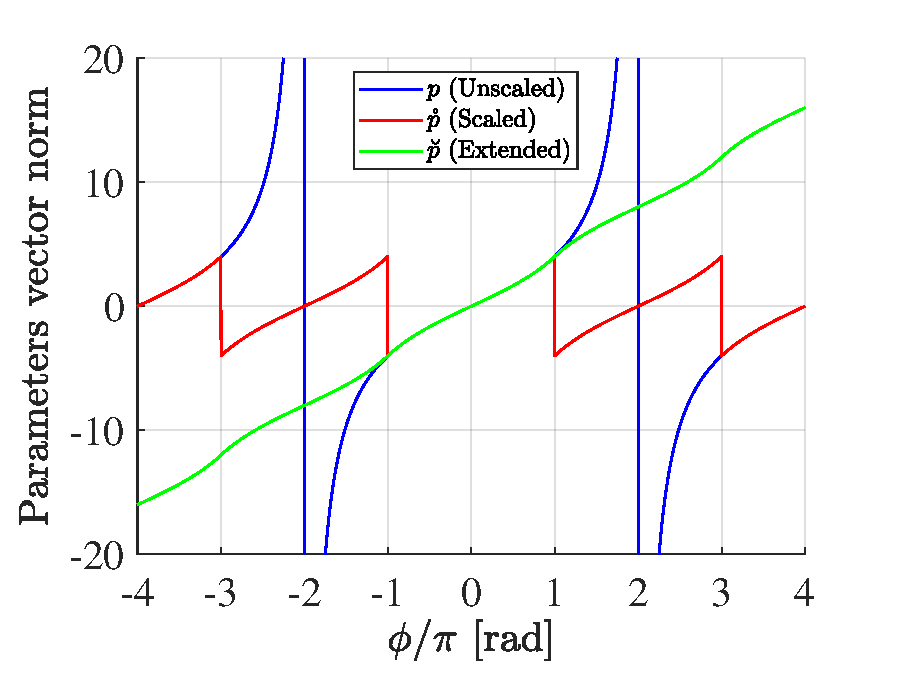
\includegraphics[width=0.85\linewidth, trim={0cm 0cm 0cm 0cm}, clip]{figures/WM_sets.pdf}
    \label{fig_params_vs_phi}
\end{figure}

Therefore, taking the extended set of Wiener-Milenkovi\'{c} rotation parameters, $\pext$, for the parametrization of the rotation variables, the rescaling operation taking place for $|\phi| > \pi$ is achieved by rewriting \cref{eq:def_gext} to yield
\begin{equation}
    \pscaled = \lambda\pext \ \ ,
    \label{eq:pscaled_and_pext}
\end{equation}
where 
\begin{equation}
    \lambda = 1 - \frac{8|q|}{|\pextnorm|} \ \ ,
    \label{eq:scaling_fac}
\end{equation}
is the \textit{scaling factor} relating the two sets, and the fact that $|\pscalednorm| < 4$ allows the simplification that
\begin{equation}
     |q| = \text{round}\left\{\frac{|\pextnorm|}{8}\right\} - \cancelto{0}{\text{round}\left\{\frac{|\pscalednorm|}{8}\right\}} = \text{round}\left\{\frac{|\pextnorm|}{8}\right\} \ \ .
    \label{eq:q}
\end{equation}

Note that since $\uvec{n}$ is unknown, only the absolute value of $\pextnorm$ and $\pscalednorm$ ($|\pextnorm|$ and $|\pscalednorm|$) can be determined from $\pext$ and $\pscaled$. Furthermore, once this rescaling is done, it is easy to rewrite \cref{eq:def_pext} to extract the absolute value of the unbounded rotation angle as
\begin{equation}
     |\phiscl| = 4\arctan{\lp\frac{\pextnorm-8|q|}{4}\rp} + 2\pi|q| \ \ .
    \label{eq:phi2}
\end{equation}

The calculations for the rotation tensor and tangent operator tensor then proceed based on the scaled set, $\pscaled$, which is a set of Wiener-Milenkovi\'{c} parameters written in the standard form. The derivatives of the tensors, however, have to be performed with respect to the extended set, $\pext$. From \cref{eq:pscaled_and_pext}, it can be inferred that
\begin{equation}
    \del{\pscaled}{\pext} = \del{\lambda}{\pext} \pext^\T + \lambda\Ithree \ \ .
    \label{eq:dpscaled_dpext}
\end{equation}

Using \cref{eq:scaling_fac} and the fact that the derivative of the rounding operator's output with respect to its input is zero, the derivative of the scaling factor with respect to the extended set may be written as
\begin{align}
    \del{\lambda}{\pext} &= -8\lb \del{\lp1/\sqrt{\pext^\T\pext}\rp}{\pext}q + \cancelto{\zv}{\del{q}{\pext}}\frac{1}{\pextnorm} \rb
    \nonumber \\
     &= -8q\lb-\frac{2\pext}{2\lp\sqrt{\pext^\T\pext}\rp^3}\rb
     \nonumber \\
     &= \lp\frac{8q}{\pextnorm^3}\rp\pext
     \nonumber \\
     &= \lp\frac{1-\lambda}{\pextnorm^2}\rp \pext   \ \ ,
    \label{eq:dlambda_dpext}
\end{align}
which becomes indeterminate when $\pextnorm = 0$ and $\lambda = 1$, that is, when $\pext = \zv$. In this case, $\partial\lambda/\partial\pext = \zv$.

The operation of differentiation to $\pext$ then follows by application of the chain rule to find
\begin{align}
    \del{\lp\cdot\rp}{\pext} &= \del{\lp\cdot\rp}{\pscaled} \del{\pscaled}{\pext} 
    \nonumber \\
    &= \del{\lp\cdot\rp}{\pscaled} \lb \lp\frac{1-\lambda}{\pextnorm^2}\rp \pext\;\pext^\T + \lambda\Ithree \rb \ \ ,
    \label{eq:dpext}
\end{align}
in which \cref{eq:dpscaled_dpext,eq:dlambda_dpext} were used. In the following, the explicit expressions for the rotation and tangent operator tensors are derived, as well as their derivatives concerning the rotation parameters vector.

\subsection{Rotation and tangent operator tensors, and their derivatives}

The rotation tensor and tangent operator tensors depend only on the rotation angle and the axis of rotation. Since those are the same for the unscaled, scaled and extended sets, $\p$, $\pscaled$ and $\pext$, it follows that $\R(\p) = \R(\pscaled) = \R(\pext)$ and $\H(\p) = \H(\pscaled) = \H(\pext)$. Therefore, expressions for the rotation tensor, the tangent operator tensor's transpose, and its inverse, in terms of the \textit{scaled set} of Wiener-Milenkovi\'{c} parameters may be respectively written, after manipulation of the definitions given by \citeonline{bauchau2011flexible}, as
\begin{alignat}{2}
    \R &= \upsilon^2 \lb \lp\frac{1}{\upsilon^2}-2\pscalednorm^2\rp\Ithree + 2\pscaled\;\pscaled^\T + 2p_0\ptilscl \rb &&= \upsilon^2\Th \ \ ,
    \label{eq:R_WM}
    \\
    \HT &= 2\upsilon^2 \lp p_0\Ithree + \frac{1}{4}\pscaled\;\pscaled^\T - \ptilscl \rp &&= \upsilon^2\tens{\Psi} \ \ ,
    \label{eq:HT_WM}
    \\
    \HinvT &= \frac{1}{2}\lp p_0\Ithree + \frac{1}{4}\pscaled\;\pscaled^\T + \ptilscl  \rp \ \ ,
    \label{eq:HinvT_WM}
\end{alignat}
in which 
\begin{align}
    p_0 = 2 - \frac{\pscalednorm}{8} \ \ ,
    \label{eq:p0}
\end{align}
and 
\begin{align}
    \upsilon = \lp4-p_0\rp^{-1} \ \ .
    \label{eq:upsilon}
\end{align}

Since the rotation parametrization of the rotation variables is performed in terms of the \textit{extended set}, the derivatives have to be taken with respect to it. Therefore, taking a derivative of the tensors in \cref{eq:R_WM,eq:HT_WM,eq:HinvT_WM} with respect to $\pext$ yields
\begin{alignat}{2}
    \del{\R}{\pext} &= \del{\R}{\pscaled}\del{\pscaled}{\pext} 
    &&= \lp\del{\upsilon^2}{\pscaled}\Th+\upsilon^2\del{\Th}{\pscaled}\rp\del{\pscaled}{\pext} \ \ ,
    \label{eq:dR_dpext}
    \\
    \del{\HT}{\pext} &= \del{\HT}{\pscaled}\del{\pscaled}{\pext} &&= \lp\del{\upsilon^2}{\pscaled}\tens{\Psi}+\upsilon^2\del{\tens{\Psi}}{\pscaled}\rp\del{\pscaled}{\pext} \ \ ,
    \label{eq:dHT_dpext}
    \\
    \del{\HinvT}{\pext} &= \del{\HinvT}{\pscaled}\del{\pscaled}{\pext} \ \ ,
    \label{eq:dHinvT_dpext}
\end{alignat}
where 
\begin{align}
    \del{\upsilon^2}{\pscaled} &= \del{\upsilon^2}{p_0}\del{p_0}{\pscaled} 
    \nonumber \\
    &= \lb2\lp4-p_0\rp^{-3}\rb \lp -\frac{\pscaled}{4} \rp 
    \nonumber \\
    &= -\frac{\upsilon^3\pscaled}{2} \ \ ,
    \label{eq:dups_dpscaled}
\end{align}
and $\partial\pscaled/\partial\pext$ is given in \cref{eq:dpext}.

The time derivative of the rotation tensor is given by
\begin{align}
    \Rdot = \del{\R}{t} = \del{\R}{\pscaled}\del{\pscaled}{t} \ \ ,
    \label{eq:dR_dt}
\end{align}
in which 
\begin{align}
    \del{\pscaled}{t} &= \del{\pscaled}{\pext}\del{\pext}{t}
    \nonumber \\
    &= \lb \lp\frac{1-\lambda}{\pextnorm^2}\rp \pext\;\pext^\T + \lambda\Ithree \rb \pextdot \ \ ,
    \label{eq:dpscl_dt}
\end{align}
where $\pextdot = \partial\pext/\partial t$ is the time derivative of the extended rotation parameters set.

Furthermore, the derivative with respect to $\pext$ of the time derivative of the rotation tensor, $\Rdot\lp\pext,\pextdot\rp$, may be written as
\begin{align}
    \del{\Rdot}{\pext} &= \del{\Rdot}{\pscaled}\del{\pscaled}{\pext} + \del{\Rdot}{\pextdot}\cancelto{\zthree}{\del{\pextdot}{\pext}} 
    \nonumber \\
    &= \del{}{\pscaled}\lp\del{\R}{\pscaled}\del{\pscaled}{t}\rp\del{\pscaled}{\pext}  
    \nonumber \\
    &= \lb\frac{\partial^2\R}{\lp\partial\pscaled\rp^2}\del{\pscaled}{t}+\del{\R}{\pscaled}\cancelto{\zthree}{\del{}{t}\lp\del{\pscaled}{\pscaled}\rp}\rb\del{\pscaled}{\pext}
    \nonumber \\
    &= \lb\frac{\partial^2\R}{\lp\partial\pscaled\rp^2}\del{\pscaled}{t}\rb\del{\pscaled}{\pext} \ \ ,
    \label{eq:dRdot_dpext}
\end{align}
in which $\partial\pextdot/\partial\pext = \zthree$ stems from the fact that $\pextdot$ is not a function of $\pext$, and $\del{}{t}\lp\partial\pscaled/\partial\pscaled\rp$ is the time derivative of the identity tensor, which is the zero tensor. An expression for $\partial^2\R/\lp\partial\pscaled\rp^2$ may be found by taking a derivative with respect to $\pext$ of \cref{eq:dR_dpext}, yielding
\begin{align}
    \frac{\partial^2\R}{\lp\partial\pscaled\rp^2} &=  \lb\frac{\partial^2\upsilon}{\lp\partial\pscaled\rp^2}\Th + \del{\upsilon^2}{\pscaled}\del{\Th}{\pscaled} + \del{\upsilon^2}{\pscaled}\del{\Th}{\pscaled} + \upsilon^2\frac{\partial^2\Th}{\lp\partial\pscaled\rp^2}\rb\del{\pscaled}{\pext} + \lp\del{\upsilon^2}{\pscaled}\Th+\upsilon^2\del{\Th}{\pscaled}\rp \cancelto{\zthree}{\del{}{\pscaled}\lp\del{\pscaled}{\pext}\rp}
    \nonumber \\
    &=  \lb\frac{\partial^2\upsilon}{\lp\partial\pscaled\rp^2}\Th + \del{\upsilon^2}{\pscaled}\del{\Th}{\pscaled} + \del{\upsilon^2}{\pscaled}\del{\Th}{\pscaled} + \upsilon^2\frac{\partial^2\Th}{\lp\partial\pscaled\rp^2}\rb\del{\pscaled}{\pext} \ \ ,
    \label{eq:d2R_dpext2}
\end{align}
in which $\del{}{\pscaled}\lp\partial\pscaled/\partial\pext\rp$ yields the derivative of the identity tensor with respect to $\pext$, which is the zero tensor, and where
\begin{align}
    \frac{\partial^2\upsilon}{\lp\partial\pscaled\rp^2} &= \del{}{\pscaled} \lb-\frac{1}{2}\lp4-p_0\rp^{-3}\pext\rb
    \nonumber \\
    &= -\frac{1}{2}\lp4-p_0\rp^{-3}\Ithree + \frac{3}{2}\lp4-p_0\rp^{-4}\lp\frac{\pscaled}{4}\rp\pscaled^\T
    \nonumber \\
    &= -\frac{1}{2}\lp4-p_0\rp^{-3} \lb \Ithree - \frac{3}{4}\lp4-p_0\rp^{-1}\pscaled\;\pscaled^\T \rb
    \nonumber \\
    &= -\frac{\upsilon^3}{2} \lp \Ithree - \frac{3\upsilon}{4}\pscaled\;\pscaled^\T \rp \ \ ,
    \label{eq:d2ups_dpscaled2}
\end{align}
is obtained by taking a derivative of \cref{eq:dups_dpscaled} with respect to $\pscaled$.

If one lets $\pscaled=\{p_1,p_2,p_3\}^\T$, an expansion of $\Th$ in \cref{eq:R_WM} leads to
\begin{align}
    \Th &= 
    \begin{bmatrix}
    p_0^2+p_1^2-p_2^2-p_3^2 & 2\lp p_1p_2-p_0p_3 \rp & 2\lp p_1p_3+p_0p_2 \rp
    \\ 
     2\lp p_1p_2+p_0p_3 \rp & p_0^2-p_1^2+p_2^2-p_3^2 & 2\lp p_2p_3-p_0p_1 \rp
    \\ 
    2\lp p_1p_3-p_0p_2 \rp & 2\lp p_2p_3+p_0p_1 \rp & p_0^2-p_1^2-p_2^2+p_3^2
    \end{bmatrix} \ \ .
    \label{eq:T_explicit}
\end{align}

Then, explicit expressions for the components of the third-order tensor $\partial\Th/\partial\pscaled$ in \cref{eq:dR_dpext} are
\begin{align}
    \del{\Th}{p_1} &= 
    2\begin{bmatrix}
    p_1\lp1-p_0/4\rp & p_2+p_1p_3/4 & p_3-p_1p_2/4
    \\ 
    p_2-p_1p_3/4 & -p_1\lp1+p_0/4\rp & -\lp p_0-p_1^2/4\rp
    \\ 
    p_3+p_1p_2/4 & p_0-p_1^2/4 & -p_1\lp1+p_0/4\rp
    \end{bmatrix} \ \ ,
    \label{eq:dT_dp1}
    \\
    \del{\Th}{p_2} &= 
    2\begin{bmatrix}
    -p_2\lp1+p_0/4\rp & p_1+p_2p_3/4 & p_0-p_2^2/4
    \\ 
    p_1-p_2p_3/4 & p_2\lp1-p_0/4\rp & p_3+p_1p_2/4
    \\ 
    -\lp p_0-p_2^2/4\rp & p_3-p_1p_2/4 & -p_2\lp1+p_0/4\rp
    \end{bmatrix} \ \ ,
    \label{eq:dT_dp2}
    \\
    \del{\Th}{p_3} &= 
    2\begin{bmatrix}
    -p_3\lp1+p_0/4\rp & -\lp p_0-p_3^2/4\rp & p_1-p_2p_3/4
    \\ 
    p_0-p_3^2/4 & -p_3\lp1+p_0/4\rp & p_2+p_1p_3/4
    \\ 
    p_1+p_2p_3/4 & p_2-p_1p_3/4 & p_3\lp1-p_0/4\rp
    \end{bmatrix} \ \ ,
    \label{eq:dT_dp3}
\end{align}
whereas the components of the fourth-order tensor $\partial^2\Th/\lp\partial\pscaled\rp^2$ in \cref{eq:d2R_dpext2} are
\begin{align}
    \frac{\partial^2\Th}{\partial p_1\partial p_1} &= 
    2\begin{bmatrix}
    \lp1-p_0/4\rp+p_1^2/16 & p_3/4 & -p_2/4
    \\ 
    -p_3/4 & -\lp1+p_0/4\rp+p_1^2/16 & 3p_1/4
    \\ 
    p_2/4 & -3p_1/4 & -\lp1+p_0/4\rp+p_1^2/16
    \end{bmatrix} \ \ ,
    \label{eq:dT_dp1dp1}
    \\
    \frac{\partial^2\Th}{\partial p_2\partial p_2} &= 
    2\begin{bmatrix}
    -\lp1+p_0/4\rp+p_2^2/16 & p_3/4 & -3p_2/4
    \\ 
    -p_3/4 & \lp1-p_0/4\rp+p_2^2/16 & p_1/4
    \\ 
    3p_2/4 & -p_1/4 & -\lp1+p_0/4\rp+p_2^2/16
    \end{bmatrix} \ \ ,
    \label{eq:dT_dp2dp2}
    \\
    \frac{\partial^2\Th}{\partial p_3\partial p_3} &= 
    2\begin{bmatrix}
    -\lp1+p_0/4\rp+p_3^2/16 & 3p_3/4 & -p_2/4
    \\ 
    -3p_3/4 & -\lp1+p_0/4\rp+p_3^2/16 & p_1/4
    \\ 
    p_2/4 & -p_1/4 & \lp1-p_0/4\rp+p_3^2/16
    \end{bmatrix} \ \ ,
    \label{eq:dT_dp3dp3}
    \\
    \frac{\partial^2\Th}{\partial p_1\partial p_2} &= 
    2\begin{bmatrix}
    p_1p_2/16 & 1 & -p_1/4
    \\ 
    1 & p_1p_2/16 & p_2/4
    \\ 
    p_1/4 & -p_2/4 & p_1p_2/16
    \end{bmatrix} \ \ ,
    \label{eq:dT_dp1dp2}
    \\
    \frac{\partial^2\Th}{\partial p_1\partial p_3} &= 
    2\begin{bmatrix}
    p_1p_3/16 & -p_1/4 & 1
    \\ 
    -p_1/4 & p_1p_3/16 & p_3/4
    \\ 
    1 & -p_3/4 & p_1p_3/16
    \end{bmatrix} \ \ ,
    \label{eq:dT_dp1dp3}
    \\
    \frac{\partial^2\Th}{\partial p_2\partial p_3} &= 
    2\begin{bmatrix}
    p_2p_3/16 & p_2/4 & -p_3/4
    \\ 
    -p_2/4 & p_2p_3/16 & 1
    \\ 
    p_3/4 & 1 & p_2p_3/16
    \end{bmatrix} \ \ ,
    \label{eq:dT_dp2dp3}
\end{align}
and, of course, $\partial\Th/\partial p_i\partial p_j = \partial\Th/\partial p_j\partial p_i$, for $i,j = (1,2,3)$, since these are continuous functions.

Also, the components of the third-order tensor $\partial\tens{\Psi}/\partial\pscaled$ in \cref{eq:dHT_dpext} are
\begin{align}
    \del{\tens{\Psi}}{p_1} &= 
    \frac{1}{2}\begin{bmatrix}
    p_1 & p_2 & p_3
    \\ 
    p_2 & -p_1 & 4
    \\ 
    p_3 & -4 & -p_1
    \end{bmatrix} \ \ ,
    \label{eq:dPsi_dp1}
    \\
    \del{\tens{\Psi}}{p_2} &= 
    \frac{1}{2}\begin{bmatrix}
    -p_2 & p_1 & -4
    \\ 
    p_1 & p_2 & p_3
    \\ 
    4 & p_3 & -p_2
    \end{bmatrix} \ \ ,
    \label{eq:dPsi_dp2}
    \\
    \del{\tens{\Psi}}{p_3} &= 
    \frac{1}{2}\begin{bmatrix}
    -p_3 & 4 & p_1
    \\ 
    -4 & -p_3 & p_2
    \\ 
    p_1 & p_2 & p_3
    \end{bmatrix} \ \ ,
    \label{eq:dPsi_dp3}
\end{align}
whereas the components of the third-order tensor $\partial\HinvT/\partial\pscaled$ in \cref{eq:dHinvT_dpext} are
\begin{align}
    \del{\HinvT}{p_1} &= 
    \frac{1}{8}\begin{bmatrix}
    p_1 & p_2 & p_3
    \\ 
    p_2 & -p_1 & -4
    \\ 
    p_3 & 4 & -p_1
    \end{bmatrix} \ \ ,
    \label{eq:dHinvT_dp1}
    \\
    \del{\HinvT}{p_2} &= 
    \frac{1}{8}\begin{bmatrix}
    -p_2 & p_1 & 4
    \\ 
    p_1 & p_2 & p_3
    \\ 
    -4 & p_3 & -p_2
    \end{bmatrix} \ \ ,
    \label{eq:dHinvT_dp2}
    \\
    \del{\HinvT}{p_3} &= 
    \frac{1}{8}\begin{bmatrix}
    -p_3 & -4 & p_1
    \\ 
    4 & -p_3 & p_2
    \\ 
    p_1 & p_2 & p_3
    \end{bmatrix} \ \ .
    \label{eq:dHinvT_dp3}
\end{align}

\Cref{eq:R_WM,eq:HT_WM,eq:HinvT_WM,eq:dR_dt,eq:dR_dpext,eq:dHT_dpext,eq:dHinvT_dpext,eq:dRdot_dpext} provide the expressions to be used in the construction of the system's residual array, and Jacobian and inertia matrices, since the generic elemental and nodal rotation parameters, $\pe$, and $\p_n$ (or $\phat_n$) are actually represented by extended sets of Wiener-Milenkovi\'{c} parameters.


\end{apendicesenv}


% Bibliography
\bibliography{references}

\end{document}
